% Options for packages loaded elsewhere
\PassOptionsToPackage{unicode}{hyperref}
\PassOptionsToPackage{hyphens}{url}
\PassOptionsToPackage{dvipsnames,svgnames,x11names}{xcolor}
%
\documentclass[
  letterpaper,
  DIV=11,
  numbers=noendperiod]{scrreprt}

\usepackage{amsmath,amssymb}
\usepackage{lmodern}
\usepackage{iftex}
\ifPDFTeX
  \usepackage[T1]{fontenc}
  \usepackage[utf8]{inputenc}
  \usepackage{textcomp} % provide euro and other symbols
\else % if luatex or xetex
  \usepackage{unicode-math}
  \defaultfontfeatures{Scale=MatchLowercase}
  \defaultfontfeatures[\rmfamily]{Ligatures=TeX,Scale=1}
\fi
% Use upquote if available, for straight quotes in verbatim environments
\IfFileExists{upquote.sty}{\usepackage{upquote}}{}
\IfFileExists{microtype.sty}{% use microtype if available
  \usepackage[]{microtype}
  \UseMicrotypeSet[protrusion]{basicmath} % disable protrusion for tt fonts
}{}
\makeatletter
\@ifundefined{KOMAClassName}{% if non-KOMA class
  \IfFileExists{parskip.sty}{%
    \usepackage{parskip}
  }{% else
    \setlength{\parindent}{0pt}
    \setlength{\parskip}{6pt plus 2pt minus 1pt}}
}{% if KOMA class
  \KOMAoptions{parskip=half}}
\makeatother
\usepackage{xcolor}
\setlength{\emergencystretch}{3em} % prevent overfull lines
\setcounter{secnumdepth}{5}
% Make \paragraph and \subparagraph free-standing
\ifx\paragraph\undefined\else
  \let\oldparagraph\paragraph
  \renewcommand{\paragraph}[1]{\oldparagraph{#1}\mbox{}}
\fi
\ifx\subparagraph\undefined\else
  \let\oldsubparagraph\subparagraph
  \renewcommand{\subparagraph}[1]{\oldsubparagraph{#1}\mbox{}}
\fi

\usepackage{color}
\usepackage{fancyvrb}
\newcommand{\VerbBar}{|}
\newcommand{\VERB}{\Verb[commandchars=\\\{\}]}
\DefineVerbatimEnvironment{Highlighting}{Verbatim}{commandchars=\\\{\}}
% Add ',fontsize=\small' for more characters per line
\usepackage{framed}
\definecolor{shadecolor}{RGB}{241,243,245}
\newenvironment{Shaded}{\begin{snugshade}}{\end{snugshade}}
\newcommand{\AlertTok}[1]{\textcolor[rgb]{0.68,0.00,0.00}{#1}}
\newcommand{\AnnotationTok}[1]{\textcolor[rgb]{0.37,0.37,0.37}{#1}}
\newcommand{\AttributeTok}[1]{\textcolor[rgb]{0.40,0.45,0.13}{#1}}
\newcommand{\BaseNTok}[1]{\textcolor[rgb]{0.68,0.00,0.00}{#1}}
\newcommand{\BuiltInTok}[1]{\textcolor[rgb]{0.00,0.23,0.31}{#1}}
\newcommand{\CharTok}[1]{\textcolor[rgb]{0.13,0.47,0.30}{#1}}
\newcommand{\CommentTok}[1]{\textcolor[rgb]{0.37,0.37,0.37}{#1}}
\newcommand{\CommentVarTok}[1]{\textcolor[rgb]{0.37,0.37,0.37}{\textit{#1}}}
\newcommand{\ConstantTok}[1]{\textcolor[rgb]{0.56,0.35,0.01}{#1}}
\newcommand{\ControlFlowTok}[1]{\textcolor[rgb]{0.00,0.23,0.31}{#1}}
\newcommand{\DataTypeTok}[1]{\textcolor[rgb]{0.68,0.00,0.00}{#1}}
\newcommand{\DecValTok}[1]{\textcolor[rgb]{0.68,0.00,0.00}{#1}}
\newcommand{\DocumentationTok}[1]{\textcolor[rgb]{0.37,0.37,0.37}{\textit{#1}}}
\newcommand{\ErrorTok}[1]{\textcolor[rgb]{0.68,0.00,0.00}{#1}}
\newcommand{\ExtensionTok}[1]{\textcolor[rgb]{0.00,0.23,0.31}{#1}}
\newcommand{\FloatTok}[1]{\textcolor[rgb]{0.68,0.00,0.00}{#1}}
\newcommand{\FunctionTok}[1]{\textcolor[rgb]{0.28,0.35,0.67}{#1}}
\newcommand{\ImportTok}[1]{\textcolor[rgb]{0.00,0.46,0.62}{#1}}
\newcommand{\InformationTok}[1]{\textcolor[rgb]{0.37,0.37,0.37}{#1}}
\newcommand{\KeywordTok}[1]{\textcolor[rgb]{0.00,0.23,0.31}{#1}}
\newcommand{\NormalTok}[1]{\textcolor[rgb]{0.00,0.23,0.31}{#1}}
\newcommand{\OperatorTok}[1]{\textcolor[rgb]{0.37,0.37,0.37}{#1}}
\newcommand{\OtherTok}[1]{\textcolor[rgb]{0.00,0.23,0.31}{#1}}
\newcommand{\PreprocessorTok}[1]{\textcolor[rgb]{0.68,0.00,0.00}{#1}}
\newcommand{\RegionMarkerTok}[1]{\textcolor[rgb]{0.00,0.23,0.31}{#1}}
\newcommand{\SpecialCharTok}[1]{\textcolor[rgb]{0.37,0.37,0.37}{#1}}
\newcommand{\SpecialStringTok}[1]{\textcolor[rgb]{0.13,0.47,0.30}{#1}}
\newcommand{\StringTok}[1]{\textcolor[rgb]{0.13,0.47,0.30}{#1}}
\newcommand{\VariableTok}[1]{\textcolor[rgb]{0.07,0.07,0.07}{#1}}
\newcommand{\VerbatimStringTok}[1]{\textcolor[rgb]{0.13,0.47,0.30}{#1}}
\newcommand{\WarningTok}[1]{\textcolor[rgb]{0.37,0.37,0.37}{\textit{#1}}}

\providecommand{\tightlist}{%
  \setlength{\itemsep}{0pt}\setlength{\parskip}{0pt}}\usepackage{longtable,booktabs,array}
\usepackage{calc} % for calculating minipage widths
% Correct order of tables after \paragraph or \subparagraph
\usepackage{etoolbox}
\makeatletter
\patchcmd\longtable{\par}{\if@noskipsec\mbox{}\fi\par}{}{}
\makeatother
% Allow footnotes in longtable head/foot
\IfFileExists{footnotehyper.sty}{\usepackage{footnotehyper}}{\usepackage{footnote}}
\makesavenoteenv{longtable}
\usepackage{graphicx}
\makeatletter
\def\maxwidth{\ifdim\Gin@nat@width>\linewidth\linewidth\else\Gin@nat@width\fi}
\def\maxheight{\ifdim\Gin@nat@height>\textheight\textheight\else\Gin@nat@height\fi}
\makeatother
% Scale images if necessary, so that they will not overflow the page
% margins by default, and it is still possible to overwrite the defaults
% using explicit options in \includegraphics[width, height, ...]{}
\setkeys{Gin}{width=\maxwidth,height=\maxheight,keepaspectratio}
% Set default figure placement to htbp
\makeatletter
\def\fps@figure{htbp}
\makeatother

\KOMAoption{captions}{tableheading}
\makeatletter
\makeatother
\makeatletter
\@ifpackageloaded{bookmark}{}{\usepackage{bookmark}}
\makeatother
\makeatletter
\@ifpackageloaded{caption}{}{\usepackage{caption}}
\AtBeginDocument{%
\ifdefined\contentsname
  \renewcommand*\contentsname{Table of contents}
\else
  \newcommand\contentsname{Table of contents}
\fi
\ifdefined\listfigurename
  \renewcommand*\listfigurename{List of Figures}
\else
  \newcommand\listfigurename{List of Figures}
\fi
\ifdefined\listtablename
  \renewcommand*\listtablename{List of Tables}
\else
  \newcommand\listtablename{List of Tables}
\fi
\ifdefined\figurename
  \renewcommand*\figurename{Figure}
\else
  \newcommand\figurename{Figure}
\fi
\ifdefined\tablename
  \renewcommand*\tablename{Table}
\else
  \newcommand\tablename{Table}
\fi
}
\@ifpackageloaded{float}{}{\usepackage{float}}
\floatstyle{ruled}
\@ifundefined{c@chapter}{\newfloat{codelisting}{h}{lop}}{\newfloat{codelisting}{h}{lop}[chapter]}
\floatname{codelisting}{Listing}
\newcommand*\listoflistings{\listof{codelisting}{List of Listings}}
\makeatother
\makeatletter
\@ifpackageloaded{caption}{}{\usepackage{caption}}
\@ifpackageloaded{subcaption}{}{\usepackage{subcaption}}
\makeatother
\makeatletter
\@ifpackageloaded{tcolorbox}{}{\usepackage[many]{tcolorbox}}
\makeatother
\makeatletter
\@ifundefined{shadecolor}{\definecolor{shadecolor}{rgb}{.97, .97, .97}}
\makeatother
\makeatletter
\makeatother
\ifLuaTeX
  \usepackage{selnolig}  % disable illegal ligatures
\fi
\IfFileExists{bookmark.sty}{\usepackage{bookmark}}{\usepackage{hyperref}}
\IfFileExists{xurl.sty}{\usepackage{xurl}}{} % add URL line breaks if available
\urlstyle{same} % disable monospaced font for URLs
\hypersetup{
  pdftitle={Quantitative Methods 2},
  pdfauthor={Ollie Ballinger},
  colorlinks=true,
  linkcolor={blue},
  filecolor={Maroon},
  citecolor={Blue},
  urlcolor={Blue},
  pdfcreator={LaTeX via pandoc}}

\title{Quantitative Methods 2}
\author{Ollie Ballinger}
\date{10/10/2022}

\begin{document}
\maketitle
\ifdefined\Shaded\renewenvironment{Shaded}{\begin{tcolorbox}[boxrule=0pt, borderline west={3pt}{0pt}{shadecolor}, breakable, sharp corners, interior hidden, frame hidden, enhanced]}{\end{tcolorbox}}\fi

\renewcommand*\contentsname{Table of contents}
{
\hypersetup{linkcolor=}
\setcounter{tocdepth}{2}
\tableofcontents
}
\bookmarksetup{startatroot}

\hypertarget{welcome}{%
\chapter*{Welcome}\label{welcome}}
\addcontentsline{toc}{chapter}{Welcome}

\hypertarget{welcome-to-basc0005---quantitative-methods-data-science-and-visualisation}{%
\section*{Welcome to BASC0005 - Quantitative Methods: Data Science and
Visualisation}\label{welcome-to-basc0005---quantitative-methods-data-science-and-visualisation}}
\addcontentsline{toc}{section}{Welcome to BASC0005 - Quantitative
Methods: Data Science and Visualisation}

This course teaches quantitative skills, with an emphasis on the context
and use of data. Students learn to focus on datasets which will allow
them to explore questions in society -- in arts, humanities, sports,
criminal justice, economics, inequality, or policy. Students are
expected to work with Python to carry out data manipulation (cleaning
and segmentation), analysis (for example, deriving descriptive
statistics) and visualisation (graphing, mapping and other forms of
visualisation). They will engage with literatures around a topic and
connect their datasets and analyses to explore and decide wider
arguments, and link their results to these contextual considerations.
Below is an outline of the course:

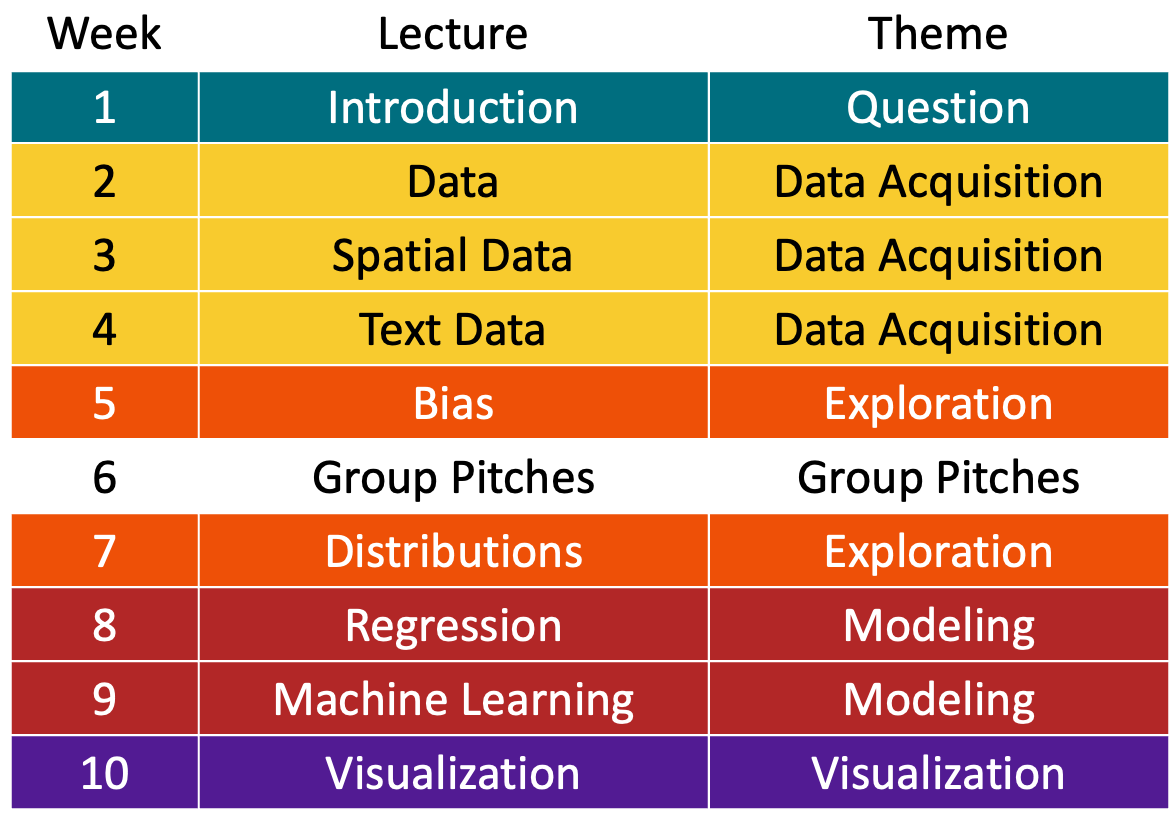
\includegraphics{./outline.png}

\bookmarksetup{startatroot}

\hypertarget{python-recap}{%
\chapter{Python Recap}\label{python-recap}}

\hypertarget{workshop-1-open-in-colab}{%
\section[\emph{Workshop 1} ]{\texorpdfstring{\emph{Workshop 1}
\href{https://colab.research.google.com/github/oballinger/QM2/blob/main/notebooks/W01.\%20Python\%20Recap.ipynb}{\protect
\includegraphics{notebooks/../colab-badge.png}}}{Workshop 1 Open In Colab}}\label{workshop-1-open-in-colab}}

\hypertarget{using-python}{%
\section{Using Python}\label{using-python}}

In this course, we'll make extensive use of \emph{Python}, a programming
language used widely in scientific computing and on the web. We will be
using Python as a way to manipulate, plot and analyse data. This isn't a
course about learning Python, it's about working with data - but we'll
learning a little bit of programming along the way.

By now, you should have done the prerequisites for the module, and
understand a bit about how Python is structured, what different commands
do, and so on - this is a bit of a refresher to remind you of what we
need at the beginning of term.

The particular flavour of Python we're using is \emph{iPython}, which,
as we've seen, allows us to combine text, code, images, equations and
figures in a \emph{Notebook}. This is a \emph{cell}, written in
\emph{markdown} - a way of writing nice text. Contrast this with
\emph{code} cell, which executes a bit of Python:

\begin{Shaded}
\begin{Highlighting}[]
\BuiltInTok{print}\NormalTok{(}\DecValTok{1}\OperatorTok{+}\DecValTok{1}\NormalTok{)}
\end{Highlighting}
\end{Shaded}

\begin{verbatim}
2
\end{verbatim}

The Notebook format allows you to engage in what Don Knuth describes as
\href{http://en.wikipedia.org/wiki/Literate_programming}{Literate
Programming}:

\begin{quote}
{[}\ldots{]} Instead of writing code containing documentation, the
literate programmer writes documentation containing code. No longer does
the English commentary injected into a program have to be hidden in
comment delimiters at the top of the file, or under procedure headings,
or at the end of lines. Instead, it is wrenched into the daylight and
made the main focus. The ``program'' then becomes primarily a document
directed at humans, with the code being herded between ``code
delimiters'' from where it can be extracted and shuffled out sideways to
the language system by literate programming tools.
\href{http://www.literateprogramming.com/lpquotes.html}{Ross Williams}
\end{quote}

\hypertarget{libraries}{%
\section{Libraries}\label{libraries}}

We will work with a number of \emph{libraries}, which provide additional
functions and techniques to help us to carry out our tasks.

These include:

\emph{Pandas:} we'll use this a lot to slice and dice data

\emph{matplotlib}: this is our basic graphing software, and we'll also
use it for mapping

\emph{nltk}: The Natural Language Tool Kit will help us work with text

We aren't doing all this to learn to program. We could spend a whole
term learning how to use Python and never look at any data, maps,
graphs, or visualisations. But we do need to understand a few basics to
use Python for working with data. So let's revisit a few concepts that
you should have covered in your prerequisites.

\hypertarget{variables}{%
\section{Variables}\label{variables}}

Python can broadly be divided in verbs and nouns: things which \emph{do}
things, and things which \emph{are} things. In Python, the verbs can be
\emph{commands}, \emph{functions}, or \emph{methods}. We won't worry too
much about the distinction here - suffice it to say, they are the parts
of code which manipulate data, calculate values, or show things on the
screen.

The simplest proper noun object in Python is the \emph{variable}.
Variables are given names and store information. This can be, for
example, numeric, text, or boolean (true/false). These are all
statements setting up variables:

n = 1

t = ``hi''

b = True

Now let's try this in code:

\begin{Shaded}
\begin{Highlighting}[]
\NormalTok{n }\OperatorTok{=} \DecValTok{1}

\NormalTok{t }\OperatorTok{=} \StringTok{"hi"}

\NormalTok{b }\OperatorTok{=} \VariableTok{True}
\end{Highlighting}
\end{Shaded}

Note that each command is on a new line; other than that, the
\emph{syntax} of Python should be fairly clear. We're setting these
variables equal to the letters and numbers and phrases and booleans.
\textbf{What's a boolean?}

The value of this is we now have values tied to these variables - so
every time we want to use it, we can refer to the variable:

\begin{Shaded}
\begin{Highlighting}[]
\NormalTok{n}
\end{Highlighting}
\end{Shaded}

\begin{verbatim}
1
\end{verbatim}

\begin{Shaded}
\begin{Highlighting}[]
\NormalTok{t}
\end{Highlighting}
\end{Shaded}

\begin{verbatim}
'hi'
\end{verbatim}

\begin{Shaded}
\begin{Highlighting}[]
\NormalTok{b}
\end{Highlighting}
\end{Shaded}

\begin{verbatim}
True
\end{verbatim}

Because we've defined these variables in the early part of the notebook,
we can use them later on.

\emph{\textbf{Advanced}: where do \textbf{classes} fit into this
noun/verb picture of variables and commands?}

\hypertarget{where-is-my-data}{%
\section{Where is my data?}\label{where-is-my-data}}

When we work in excel and text editors, we're used to seeing the data
onscreen - and if we manipulate the data in some way (averaging or
summing up), we see both the inputs and outputs on screen. The big
difference in working with Python is that we don't see our variables all
of the time, or the effect we're having on them. They're there in the
background, but it's usually worth checking in on them from time to
time, to see whether our processes are doing what we think they're
doing.

This is pretty easy to do - we can just type the variable name, or
``print(\emph{variable name})'':

\begin{Shaded}
\begin{Highlighting}[]
\NormalTok{n }\OperatorTok{=}\NormalTok{ n}\OperatorTok{+}\DecValTok{1}
\BuiltInTok{print}\NormalTok{(n)}
\BuiltInTok{print}\NormalTok{(t)}
\BuiltInTok{print}\NormalTok{(b)}
\end{Highlighting}
\end{Shaded}

\begin{verbatim}
2
hi
True
\end{verbatim}

\hypertarget{flow}{%
\section{Flow}\label{flow}}

Python, in common with all programming languages, executes commands in a
sequence - we might refer to this as the ``ineluctable march of the
machines'', but it's more common referred to as the \emph{flow} of the
code (we'll use the word ``code'' a lot - it just means commands written
in the programming language). In most cases, code just executes in the
order it's written. This is true within each \emph{cell} (each block of
text in the notebook), and it's true when we execute the cells in order;
that's why we can refer back to the variables we defined earlier:

\begin{Shaded}
\begin{Highlighting}[]
\BuiltInTok{print}\NormalTok{(n)}
\end{Highlighting}
\end{Shaded}

\begin{verbatim}
2
\end{verbatim}

If we make a change to one of these variables, say n:

\begin{Shaded}
\begin{Highlighting}[]
\NormalTok{n }\OperatorTok{=} \DecValTok{3}
\end{Highlighting}
\end{Shaded}

and execute the above ``print n'' command, you'll see that it has
changed n to 3. So if we go out of order, the obvious flow of the code
is confused. For this reason, try to write your code so it executes in
order, one cell at a time. At least for the moment, this will make it
easier to follow the logic of what you're doing to data.

\emph{Advanced}: what happens to this flow when you write
\emph{functions} to automate common tasks?

\textbf{\emph{Exercise - Setting up variables}}:

\begin{enumerate}
\def\labelenumi{\arabic{enumi}.}
\item
  Create a new cell.
\item
  Create the variables ``name'', and assign your name to it.
\item
  Create a variable ``Python'' and assign a score out of 10 to how much
  you like Python.
\item
  Create a variable ``prior'' and if you've used Python before, assign
  True; otherwise assign False to the variable
\item
  Print these out to the screen
\end{enumerate}

\hypertarget{downloading-data}{%
\section{Downloading Data}\label{downloading-data}}

Lets fetch the data we will be using for this session. There are two
ways in which you can upload data to the Colab notebook. You can use the
following code to upload a CSV or similar data file.

\begin{Shaded}
\begin{Highlighting}[]
\ImportTok{from}\NormalTok{ google.colab }\ImportTok{import}\NormalTok{ files}
\NormalTok{uploaded }\OperatorTok{=}\NormalTok{ files.upload()}
\end{Highlighting}
\end{Shaded}

\begin{verbatim}
ModuleNotFoundError: No module named 'google.colab'
\end{verbatim}

Or you can use the following cell to fetch the data directly from the
QM2 server.

Let's create a folder that we can store all our data for this session

\begin{Shaded}
\begin{Highlighting}[]
\OperatorTok{!}\NormalTok{mkdir data}
\end{Highlighting}
\end{Shaded}

\begin{Shaded}
\begin{Highlighting}[]
\OperatorTok{!}\NormalTok{mkdir .}\OperatorTok{/}\NormalTok{data}\OperatorTok{/}\NormalTok{wk1}
\OperatorTok{!}\NormalTok{curl https:}\OperatorTok{//}\NormalTok{s3.eu}\OperatorTok{{-}}\NormalTok{west}\OperatorTok{{-}}\FloatTok{2.}\ErrorTok{amazonaws}\NormalTok{.com}\OperatorTok{/}\NormalTok{qm2}\OperatorTok{/}\NormalTok{wk1}\OperatorTok{/}\NormalTok{data.csv }\OperatorTok{{-}}\NormalTok{o .}\OperatorTok{/}\NormalTok{data}\OperatorTok{/}\NormalTok{wk1}\OperatorTok{/}\NormalTok{data.csv}
\OperatorTok{!}\NormalTok{curl https:}\OperatorTok{//}\NormalTok{s3.eu}\OperatorTok{{-}}\NormalTok{west}\OperatorTok{{-}}\FloatTok{2.}\ErrorTok{amazonaws}\NormalTok{.com}\OperatorTok{/}\NormalTok{qm2}\OperatorTok{/}\NormalTok{wk1}\OperatorTok{/}\NormalTok{sample\_group.csv }\OperatorTok{{-}}\NormalTok{o .}\OperatorTok{/}\NormalTok{data}\OperatorTok{/}\NormalTok{wk1}\OperatorTok{/}\NormalTok{sample\_group.csv}
\end{Highlighting}
\end{Shaded}

\begin{verbatim}
  % Total    % Received % Xferd  Average Speed   Time    Time     Time  Current
                                 Dload  Upload   Total   Spent    Left  Speed
100   203  100   203    0     0    527      0 --:--:-- --:--:-- --:--:--   527
  % Total    % Received % Xferd  Average Speed   Time    Time     Time  Current
                                 Dload  Upload   Total   Spent    Left  Speed
100   297  100   297    0     0    838      0 --:--:-- --:--:-- --:--:--   836
\end{verbatim}

\hypertarget{storing-and-importing-data}{%
\section{Storing and importing data}\label{storing-and-importing-data}}

Typically, data we look at won't be just one number, or one bit of text.
Python has a lot of different ways of dealing with a bunch of numbers:
for example, a list of values is called a \textbf{list}:

\begin{Shaded}
\begin{Highlighting}[]
\NormalTok{listy }\OperatorTok{=}\NormalTok{ [}\DecValTok{1}\NormalTok{,}\DecValTok{2}\NormalTok{,}\DecValTok{3}\NormalTok{,}\DecValTok{6}\NormalTok{,}\DecValTok{9}\NormalTok{]}
\BuiltInTok{print}\NormalTok{(listy)}
\end{Highlighting}
\end{Shaded}

\begin{verbatim}
[1, 2, 3, 6, 9]
\end{verbatim}

A set of values \emph{linked} to an index (or key) is called a
\textbf{dictionary}; for example:

\begin{Shaded}
\begin{Highlighting}[]
\NormalTok{dicty }\OperatorTok{=}\NormalTok{ \{}\StringTok{\textquotesingle{}Bob\textquotesingle{}}\NormalTok{: }\FloatTok{1.2}\NormalTok{, }\StringTok{\textquotesingle{}Mike\textquotesingle{}}\NormalTok{: }\FloatTok{1.2}\NormalTok{, }\StringTok{\textquotesingle{}Coop\textquotesingle{}}\NormalTok{: }\FloatTok{1.1}\NormalTok{, }\StringTok{\textquotesingle{}Maddy\textquotesingle{}}\NormalTok{: }\FloatTok{1.3}\NormalTok{, }\StringTok{\textquotesingle{}Giant\textquotesingle{}}\NormalTok{: }\FloatTok{2.1}\NormalTok{\}}
\BuiltInTok{print}\NormalTok{(dicty)}
\end{Highlighting}
\end{Shaded}

\begin{verbatim}
{'Bob': 1.2, 'Mike': 1.2, 'Coop': 1.1, 'Maddy': 1.3, 'Giant': 2.1}
\end{verbatim}

Notice that the list uses square brackets with values separated by
commas, and the dict uses curly brackets with pairs separated by commas,
and colons (:) to link a \emph{key} (index or address) with a value.

(You might notice that they haven't printed out in the order you entered
them)

*\textbf{Advanced}: Print out 1) The third element of \textbf{listy},
and 2) The element of \textbf{dicty} relating to Giant

We'll discuss different ways of organising data again soon, but for now
we'll look at \emph{dataframes} - the way our data-friendly
\emph{library} \textbf{Pandas} works with data. We'll be using Pandas a
lot this term, so it's good to get started with it early.

Let's start by importing pandas. We'll also import another library, but
we're not going to worry about that too much at the moment.

If you see a warning about `Building Font Cache' don't worry - this is
normal.

\begin{Shaded}
\begin{Highlighting}[]
\ImportTok{import}\NormalTok{ pandas}

\ImportTok{import}\NormalTok{ matplotlib}
\OperatorTok{\%}\NormalTok{matplotlib inline}
\end{Highlighting}
\end{Shaded}

Let's import a simple dataset and show it in pandas. We'll use a
pre-prepared ``.csv'' file, which needs to be in the same folder as our
code.

\begin{Shaded}
\begin{Highlighting}[]
\NormalTok{data }\OperatorTok{=}\NormalTok{ pandas.read\_csv(}\StringTok{\textquotesingle{}./data/wk1/data.csv\textquotesingle{}}\NormalTok{)}
\NormalTok{data.head()}
\end{Highlighting}
\end{Shaded}

\begin{longtable}[]{@{}llllll@{}}
\toprule()
& Name & First Appearance & Approx height & Gender & Law Enforcement \\
\midrule()
\endhead
0 & Bob & 1.2 & 6.0 & Male & False \\
1 & Mike & 1.2 & 5.5 & Male & False \\
2 & Coop & 1.1 & 6.0 & Male & True \\
3 & Maddy & 1.3 & 5.5 & Female & False \\
4 & Giant & 2.1 & 7.5 & Male & False \\
\bottomrule()
\end{longtable}

What we've done here is read in a .csv file into a dataframe, the object
pandas uses to work with data, and one that has lots of methods for
slicing and dicing data, as we will see over the coming weeks. The
head() command tells iPython to show the first few columns/rows of the
data, so we can start to get a sense of what the data looks like and
what sort of type of objects is represents.

\bookmarksetup{startatroot}

\hypertarget{supplementary-kaggle-exercises}{%
\chapter{Supplementary: Kaggle
exercises}\label{supplementary-kaggle-exercises}}

If you've gotten this far, congratulations! To further hone your skills,
try working your way through the five
\href{https://www.kaggle.com/learn/intro-to-programming}{intro to
programming notebooks on Kaggle}. These cover a range of skills that
we'll be using throughout the term. Kaggle is a very useful resource for
learning data science, so making an account may not be a bad idea!

\bookmarksetup{startatroot}

\hypertarget{intro-to-pandas}{%
\chapter{Intro to Pandas}\label{intro-to-pandas}}

\hypertarget{workshop-2-open-in-colab}{%
\section[\emph{Workshop 2} ]{\texorpdfstring{\emph{Workshop 2}
\href{https://colab.research.google.com/github/oballinger/QM2/blob/main/notebooks/W02.\%20Pandas.ipynb}{\protect
\includegraphics{notebooks/../colab-badge.png}}}{Workshop 2 Open In Colab}}\label{workshop-2-open-in-colab}}

In this workshop, our aim is to get used to working with more complex
data that we've imported from external files. We'll start to graph it,
and to slice and dice it, to select the bits we're interested in.

We will work with \emph{pandas} to manipulate the data, and to derive
measures and graphs that tell us a bit more than what the source data
files tell us.

\hypertarget{aims}{%
\subsection{Aims}\label{aims}}

\begin{itemize}
\tightlist
\item
  Learn to import data to python using pandas
\item
  Learn how access specific rows, columns and cells
\item
  Plot the data
\item
  Tidy up graphs to include axes
\end{itemize}

\hypertarget{introduction}{%
\section{Introduction}\label{introduction}}

We are going to work with some UK income data. The income data is
packaged as a .csv file. The Pandas package knows how to handle this and
put the data in a DataFrame, as we've seen. Let's examine the data and
start to see what we can say about it. First of all, we have to find
data - I'm interested in looking in data with a wide spread, so I looked
for data on income in the UK.

This data is collected by the Office for National Statistics(ONS) :
http://www.ons.gov.uk/ons/datasets-and-tables/index.html?pageSize=50\&sortBy=none\&sortDirection=none\&newquery=income+percentile
- but the exact data I want to see, income by percentile, is tricky to
find.

I ended up using data from 2011, generated from a study called the
Family Resources Survey and collated and tweaked by an independent
research unit called the Institute of Fiscal Studies (IFS). The
``tweaking'' they do tends to be around the size of the family unit, and
other factors which create economies of scale - hence they
``equivalise'' it. The IFS is quoted in UK Government documents, so we
can have some trust in their impartiality, or at least accuracy - of
course, if we were publishing research about this, that's not really
good enough and we'd want to reproduce, or at least understand and
critique, their methodology rather than just trusting it!

e.g.:

http://www.ifs.org.uk/wheredoyoufitin/about.php

https://en.wikipedia.org/wiki/Equivalisation

\hypertarget{downloading-the-data}{%
\section{Downloading the Data}\label{downloading-the-data}}

Let's grab our income data from our course website and save it into our
data folder. If you've not already created a data folder then do so
using the following command. Don't worry if it generates an error, that
means you've already got a data folder.

\begin{Shaded}
\begin{Highlighting}[]
\OperatorTok{!}\NormalTok{mkdir data}
\end{Highlighting}
\end{Shaded}

\begin{verbatim}
mkdir: data: File exists
\end{verbatim}

\begin{Shaded}
\begin{Highlighting}[]
\OperatorTok{!}\NormalTok{mkdir data}\OperatorTok{/}\NormalTok{wk2}
\OperatorTok{!}\NormalTok{curl https:}\OperatorTok{//}\NormalTok{s3.eu}\OperatorTok{{-}}\NormalTok{west}\OperatorTok{{-}}\FloatTok{2.}\ErrorTok{amazonaws}\NormalTok{.com}\OperatorTok{/}\NormalTok{qm2}\OperatorTok{/}\NormalTok{wk2}\OperatorTok{/}\NormalTok{incomes.csv }\OperatorTok{{-}}\NormalTok{o .}\OperatorTok{/}\NormalTok{data}\OperatorTok{/}\NormalTok{wk2}\OperatorTok{/}\NormalTok{incomes.csv}
\end{Highlighting}
\end{Shaded}

\begin{verbatim}
mkdir: data/wk2: File exists
  % Total    % Received % Xferd  Average Speed   Time    Time     Time  Current
                                 Dload  Upload   Total   Spent    Left  Speed
100 15154  100 15154    0     0   135k      0 --:--:-- --:--:-- --:--:--  143k
\end{verbatim}

\begin{Shaded}
\begin{Highlighting}[]
\ImportTok{import}\NormalTok{ pandas}
\ImportTok{import}\NormalTok{ pylab}
\ImportTok{import}\NormalTok{ matplotlib.pyplot }\ImportTok{as}\NormalTok{ plt}
\CommentTok{\# make the plots a little wider by default}
\OperatorTok{\%}\NormalTok{matplotlib inline}
\NormalTok{plt.style.use(}\StringTok{\textquotesingle{}ggplot\textquotesingle{}}\NormalTok{)}

\NormalTok{pylab.rcParams[}\StringTok{\textquotesingle{}figure.figsize\textquotesingle{}}\NormalTok{] }\OperatorTok{=}\NormalTok{ (}\FloatTok{10.}\NormalTok{, }\FloatTok{8.}\NormalTok{)}
\end{Highlighting}
\end{Shaded}

\begin{Shaded}
\begin{Highlighting}[]
\NormalTok{data\_path }\OperatorTok{=} \StringTok{"./data/wk2/incomes.csv"}

\NormalTok{income }\OperatorTok{=}\NormalTok{  pandas.read\_csv(data\_path, index\_col}\OperatorTok{=}\DecValTok{0}\NormalTok{)}
\NormalTok{income.head()}
\end{Highlighting}
\end{Shaded}

\begin{longtable}[]{@{}llllllllllllllll@{}}
\toprule()
& Net equivalised household income in 2010-11, week & Childless couple,
annual income & Couple, two children under 14 & Couple, three children
under 14 & Couple with one child under 14 & Couple with two children
aged 15 to 18 & Couple, two children under 14 plus dependent adult &
Single adult & Lone parent, one child under 14 & Lone parent, two
children under 14 & Lone parent, two children aged 15-18 & ANNOTATIONS &
1979 to 1996-97 & 1996-97 to 2009-10 & 1996-97 to 2010-11 \\
Percentile Point & & & & & & & & & & & & & & & \\
\midrule()
\endhead
1 & 33.50 & 1,746.92 & 2,445.69 & 2,795.08 & 2,096.31 & 2,899.89 &
3,022.18 & 1,170.44 & 1,519.82 & 1,869.21 & 2,323.41 & NaN & NaN & NaN &
NaN \\
2 & 98.60 & 5,141.01 & 7,197.41 & 8,225.61 & 6,169.21 & 8,534.07 &
8,893.95 & 3,444.48 & 4,472.68 & 5,500.88 & 6,837.54 & NaN & -0.20\% &
-1.30\% & -0.50\% \\
3 & 128.56 & 6,703.11 & 9,384.36 & 10,724.98 & 8,043.74 & 11,127.17 &
11,596.39 & 4,491.09 & 5,831.71 & 7,172.33 & 8,915.14 & NaN & 0.40\% &
0.10\% & 0.10\% \\
4 & 151.05 & 7,875.75 & 11,026.05 & 12,601.20 & 9,450.90 & 13,073.75 &
13,625.05 & 5,276.75 & 6,851.90 & 8,427.05 & 10,474.75 & NaN & 0.50\% &
0.80\% & 0.60\% \\
5 & 166.32 & 8,671.91 & 12,140.68 & 13,875.06 & 10,406.30 & 14,395.38 &
15,002.41 & 5,810.18 & 7,544.57 & 9,278.95 & 11,533.65 & NaN & 0.70\% &
1.00\% & 0.90\% \\
\bottomrule()
\end{longtable}

This is a simple dataframe - we see the percentile and an income. Note
that I've told pandas to use the first column (the Percentile) as the
index to make life easier.

The percentile tells us how people on that income rank - so the final
category, 99\% (which is really binned, so 99\%\textless n\(\leq\)
100\%), is telling us how much ``the 1\%'' earn. Let's find out:

\begin{Shaded}
\begin{Highlighting}[]
\NormalTok{income.tail()}
\end{Highlighting}
\end{Shaded}

\begin{longtable}[]{@{}llllllllllllllll@{}}
\toprule()
& Net equivalised household income in 2010-11, week & Childless couple,
annual income & Couple, two children under 14 & Couple, three children
under 14 & Couple with one child under 14 & Couple with two children
aged 15 to 18 & Couple, two children under 14 plus dependent adult &
Single adult & Lone parent, one child under 14 & Lone parent, two
children under 14 & Lone parent, two children aged 15-18 & ANNOTATIONS &
1979 to 1996-97 & 1996-97 to 2009-10 & 1996-97 to 2010-11 \\
Percentile Point & & & & & & & & & & & & & & & \\
\midrule()
\endhead
95 & 1075.73 & 56,088.56 & 78,523.99 & 89,741.70 & 67,306.27 & 93,107.01
& 97,033.21 & 37,579.34 & 48,797.05 & 60,014.76 & 74,597.79 & NaN &
2.90\% & 2.00\% & 1.30\% \\
96 & 1174.48 & 61,237.18 & 85,732.05 & 97,979.49 & 73,484.61 &
101,653.72 & 105,940.32 & 41,028.91 & 53,276.35 & 65,523.78 & 81,445.45
& NaN & 3.00\% & 2.00\% & 1.40\% \\
97 & 1302.74 & 67,925.07 & 95,095.10 & 108,680.12 & 81,510.09 &
112,755.62 & 117,510.37 & 45,509.80 & 59,094.81 & 72,679.83 & 90,340.35
& NaN & 3.20\% & 2.20\% & 1.60\% \\
98 & 1523.31 & 79,425.23 & 111,195.32 & 127,080.36 & 95,310.27 &
131,845.88 & 137,405.64 & 53,214.90 & 69,099.95 & 84,984.99 & 105,635.55
& NaN & 3.20\% & 2.70\% & 1.70\% \\
99 & 2090.35 & 108,990.74 & 152,587.04 & 174,385.19 & 130,788.89 &
180,924.64 & 188,553.99 & 73,023.80 & 94,821.95 & 116,620.10 &
144,957.69 & NaN & NaN & NaN & NaN \\
\bottomrule()
\end{longtable}

Well, they we have it - the 1\% earn, on average, about £2000 a week.
How does that compare to people in the 90\% decile? We can access
particular \emph{rows} in a dataframe using \textbf{.loc{[}row
index{]}}; because our index is the percentile point, we can just read
it off:

\begin{Shaded}
\begin{Highlighting}[]
\NormalTok{income.loc[}\DecValTok{90}\NormalTok{]}
\end{Highlighting}
\end{Shaded}

\begin{verbatim}
Net equivalised household income in 2010-11, week        845.54
Childless couple, annual income                       44,086.54
Couple, two children under 14                         61,721.15
Couple, three children under 14                       70,538.46
Couple with one child under 14                        52,903.85
Couple with two children aged 15 to 18                73,183.65
Couple, two children under 14 plus dependent adult    76,269.71
Single adult                                          29,537.98
Lone parent, one child under 14                       38,355.29
Lone parent, two children under 14                    47,172.60
Lone parent, two children aged 15-18                  58,635.10
ANNOTATIONS                                                 NaN
1979 to 1996-97                                           2.50%
1996-97 to 2009-10                                        1.70%
1996-97 to 2010-11                                        1.20%
Name: 90, dtype: object
\end{verbatim}

We can also select a range of values with the ``colon'' notation. This
will select the 90-95th percentiles, for example:

\begin{Shaded}
\begin{Highlighting}[]
\NormalTok{income.loc[}\DecValTok{90}\NormalTok{:}\DecValTok{95}\NormalTok{]}
\end{Highlighting}
\end{Shaded}

\begin{longtable}[]{@{}llllllllllllllll@{}}
\toprule()
& Net equivalised household income in 2010-11, week & Childless couple,
annual income & Couple, two children under 14 & Couple, three children
under 14 & Couple with one child under 14 & Couple with two children
aged 15 to 18 & Couple, two children under 14 plus dependent adult &
Single adult & Lone parent, one child under 14 & Lone parent, two
children under 14 & Lone parent, two children aged 15-18 & ANNOTATIONS &
1979 to 1996-97 & 1996-97 to 2009-10 & 1996-97 to 2010-11 \\
Percentile Point & & & & & & & & & & & & & & & \\
\midrule()
\endhead
90 & 845.54 & 44,086.54 & 61,721.15 & 70,538.46 & 52,903.85 & 73,183.65
& 76,269.71 & 29,537.98 & 38,355.29 & 47,172.60 & 58,635.10 & NaN &
2.50\% & 1.70\% & 1.20\% \\
91 & 876.63 & 45,707.74 & 63,990.84 & 73,132.39 & 54,849.29 & 75,874.85
& 79,074.40 & 30,624.19 & 39,765.74 & 48,907.29 & 60,791.30 & NaN &
2.60\% & 1.70\% & 1.20\% \\
92 & 911.29 & 47,514.54 & 66,520.35 & 76,023.26 & 57,017.44 & 78,874.13
& 82,200.15 & 31,834.74 & 41,337.65 & 50,840.55 & 63,194.33 & NaN &
2.60\% & 1.80\% & 1.20\% \\
93 & 957.14 & 49,905.23 & 69,867.32 & 79,848.36 & 59,886.27 & 82,842.68
& 86,336.04 & 33,436.50 & 43,417.55 & 53,398.59 & 66,373.95 & NaN &
2.70\% & 1.80\% & 1.30\% \\
94 & 1016.37 & 52,993.38 & 74,190.73 & 84,789.40 & 63,592.05 & 87,969.00
& 91,678.54 & 35,505.56 & 46,104.24 & 56,702.91 & 70,481.19 & NaN &
2.90\% & 1.90\% & 1.30\% \\
95 & 1075.73 & 56,088.56 & 78,523.99 & 89,741.70 & 67,306.27 & 93,107.01
& 97,033.21 & 37,579.34 & 48,797.05 & 60,014.76 & 74,597.79 & NaN &
2.90\% & 2.00\% & 1.30\% \\
\bottomrule()
\end{longtable}

\hypertarget{accessing-parts-of-a-dataframe}{%
\section{Accessing parts of a
dataframe}\label{accessing-parts-of-a-dataframe}}

If we want to extract the actual value instead of just the whole row, we
need to reference the \emph{column} as well as the row. In pandas,
columns are referenced by \textbf{column name}:

\begin{Shaded}
\begin{Highlighting}[]
\NormalTok{income[}\StringTok{\textquotesingle{}Net equivalised household income in 2010{-}11, week\textquotesingle{}}\NormalTok{]}
\end{Highlighting}
\end{Shaded}

\begin{verbatim}
Percentile Point
1       33.50
2       98.60
3      128.56
4      151.05
5      166.32
       ...   
95    1075.73
96    1174.48
97    1302.74
98    1523.31
99    2090.35
Name: Net equivalised household income in 2010-11, week, Length: 99, dtype: float64
\end{verbatim}

So, to access a particular cell, we tell Python the row and the column
(this is pretty simple - the same way we tell excel to access cell
``A34'' meaning Column A, Row 34). One way we do that in pandas is to
select the column, and then use .loc{[}{]} on the index.

\begin{Shaded}
\begin{Highlighting}[]
\NormalTok{income[}\StringTok{\textquotesingle{}Net equivalised household income in 2010{-}11, week\textquotesingle{}}\NormalTok{].loc[}\DecValTok{90}\NormalTok{]}
\end{Highlighting}
\end{Shaded}

\begin{verbatim}
845.54
\end{verbatim}

We've accessed row 90 of the column called `Net equivalised household
income in 2010-11, week'; can we access the data the other way around -
can we first take the row and then specify a column? Let's try:

\begin{Shaded}
\begin{Highlighting}[]
\NormalTok{income.loc[}\DecValTok{90}\NormalTok{][}\StringTok{\textquotesingle{}Net equivalised household income in 2010{-}11, week\textquotesingle{}}\NormalTok{]}
\end{Highlighting}
\end{Shaded}

\begin{verbatim}
845.54
\end{verbatim}

Yes, this seems to be working fine.

\hypertarget{extension}{%
\subsection{Extension}\label{extension}}

The reason for this is that selecting the column spits out a smaller
dataframe, and all dataframes use ``loc'', so we can use that. Another
way to do this would be to use an explicit variable for the dataframe,
along the lines of:

\texttt{smallDataFrame\ =\ income{[}\textquotesingle{}Net\ equivalised\ household\ income\ in\ 2010-11,\ week\textquotesingle{}{]}}\strut \\
\texttt{smallDataFrame.loc{[}90{]}}

by doing income

\texttt{{[}\textquotesingle{}Net\ equivalised\ household\ income\ in\ 2010-11,\ week\textquotesingle{}{]}.loc{[}90{]}}

we're taking the ``smallDataFrame'' object as an implicit (or hidden)
output

If we want to look at a few rows of data, we can use a range:

\begin{Shaded}
\begin{Highlighting}[]
\NormalTok{income[}\StringTok{\textquotesingle{}Net equivalised household income in 2010{-}11, week\textquotesingle{}}\NormalTok{].loc[}\DecValTok{90}\NormalTok{:}\DecValTok{95}\NormalTok{]}
\end{Highlighting}
\end{Shaded}

\begin{verbatim}
Percentile Point
90     845.54
91     876.63
92     911.29
93     957.14
94    1016.37
95    1075.73
Name: Net equivalised household income in 2010-11, week, dtype: float64
\end{verbatim}

So, to recap, we can now access a particular \textbf{row} using
\emph{loc{[}index number{]}}, a particular \textbf{column} with the
square brackets formalism \emph{dataframename{[}`column name'{]}}, or
both \emph{dataframename{[}`column name'{]}.loc{[}index number{]}}.
We've made a start at being able to get to the bits of data we need.

\hypertarget{exercise}{%
\section{Exercise:}\label{exercise}}

How do the equivalised incomes of single adults and childless couples
compare? Look at the 1st, 99th and 50th percentile and summarise what
this tells you about the value or price of coupling.

\hypertarget{examining-the-distribution}{%
\section{Examining the Distribution}\label{examining-the-distribution}}

Returning to the overall statistics, the 90\% percentile earns less than
half the top percentile (``the 1\%''); if you're taking home over £800
as a household, you're in the top 10\% of earners.

How does 1. The income of ``the 1\%'' compare with the mean and median
across the population, as a proportion? 2. How does the 1\% compare with
the 90th percentile (the 10\%)? 3. How does the 10\% compare with the
median and mean?

The 1\% earn about 60 times the poorest groups in society - and we've
made other comparisons. But that's not the whole story. Let's look at
the income graph.

In pandas, we can plot this fairly easily\ldots{}

\begin{Shaded}
\begin{Highlighting}[]
\NormalTok{income[}\StringTok{\textquotesingle{}Net equivalised household income in 2010{-}11, week\textquotesingle{}}\NormalTok{].plot()}
\NormalTok{plt.title(}\StringTok{\textquotesingle{}UK Net Equivalised Income by Percentile per week, 2010{-}11\textquotesingle{}}\NormalTok{)}
\NormalTok{plt.xlabel(}\StringTok{\textquotesingle{}Income Percentile\textquotesingle{}}\NormalTok{)}
\NormalTok{plt.ylabel(}\StringTok{\textquotesingle{}Income (Net, Equivalised) [GBP]\textquotesingle{}}\NormalTok{)}
\end{Highlighting}
\end{Shaded}

\begin{verbatim}
Text(0, 0.5, 'Income (Net, Equivalised) [GBP]')
\end{verbatim}

\begin{figure}[H]

{\centering \includegraphics{notebooks/W02. Pandas_files/figure-pdf/cell-13-output-2.png}

}

\end{figure}

We see a curve that is pretty linear in the middle region, but curves
rapidly upwards in the higher percentile and looks more like a power
law.

\hypertarget{exercise-means}{%
\subsection{Exercise: Means}\label{exercise-means}}

Where does the mean appear here? Draw in a horizontal line to show the
mean using \textbf{axhline}. Show the median on the same graph. What is
the meaning of the median in this context?

Hint: Recall that last time we used \emph{axvline} to highlight the mean
and standard deviation by drawing vertical lines on the axis. Here, we
use \emph{axhline} to draw horizontal lines.

\hypertarget{extension-accessing-cells}{%
\subsection{Extension: Accessing
cells}\label{extension-accessing-cells}}

There are a number of ways to access elements of the dataframe: we've
shown how to access columns by the {[}\emph{`name of column'}{]} method,
and rows via the .loc{[}\emph{index}{]} method; and how we can select a
range. There are also .iloc methods to select by number rather than
name; you should become familiar with these on the documentation page
for pandas.

\hypertarget{comparing-segments}{%
\section{Comparing segments}\label{comparing-segments}}

Earlier, we compared some summary statistics of single people and
couples. Let's look at the wider curve for more than one group, now:

\begin{Shaded}
\begin{Highlighting}[]
\CommentTok{\#This is going to throw a load of errors}
\NormalTok{income[[}\StringTok{\textquotesingle{}Single adult\textquotesingle{}}\NormalTok{,}\StringTok{\textquotesingle{}Lone parent, one child under 14\textquotesingle{}}\NormalTok{]].plot()}
\end{Highlighting}
\end{Shaded}

\begin{verbatim}
TypeError: no numeric data to plot
\end{verbatim}

\hypertarget{warning}{%
\section{Warning}\label{warning}}

This isn't looking good. There's a load of text and no graph. If you've
not seen this before, it's an error - something has gone wrong.
Generally, if we look at the \textbf{final} line, it should tell us
what's wrong, in this case there's ``no numeric data to plot'', which is
weird, because we've seen the data and have even plotted some of it.

\hypertarget{messy-data}{%
\section{Messy Data}\label{messy-data}}

DataFrames, as we are starting to see, give us the chance to plot, chop,
slice and data to help us make sense of it. Here, we will create a
\textbf{new} DataFrame to take only two columns of data, and get rid of
any blank cells and any cells which are not being read as numbers -
normally a sign of a missing value or a non-numerical character. Why
could this be happening? It could be

\begin{itemize}
\item
  due to blank spaces in the text file
\item
  due to letters where there should be numbers
\item
  due to characters (``,'', ``-'', etc) that shouldn't really be there
\end{itemize}

In general, there will be some detective work required to figure out
what's wrong in our text file. Your best bet is sometimes to open up the
data in a text editor, like I've done here:

\begin{Shaded}
\begin{Highlighting}[]
\ImportTok{from}\NormalTok{ IPython.display }\ImportTok{import}\NormalTok{ Image}

\NormalTok{data\_path }\OperatorTok{=} \StringTok{"https://s3.eu{-}west{-}2.amazonaws.com/qm2/wk2/data.png"}
\NormalTok{Image(data\_path)}
\end{Highlighting}
\end{Shaded}

\begin{figure}[H]

{\centering 
\includegraphics{notebooks/W02. Pandas_files/figure-pdf/cell-15-output-1.png}

}

\end{figure}

That's a screenshot of our datafile, opened up in a text editor. As we
can see, these numbers are separated by commas and surrounded by
quotation marks - this is normal, and what .csv files are supposed to
look like. However, there are a lot of commas within the numbers - which
makes it easier for people to read, but confuses software. Luckily,
Python has a method for dealing with this - the ``replace'' method.

Unfortunately, this dataframe is quite messy, so I'm going to have to
extract just the columns of data I'm interested in to make it work. I'll
do that by creating a new dataframe:

\hypertarget{example-cleaning-data}{%
\section{Example: Cleaning data}\label{example-cleaning-data}}

\begin{Shaded}
\begin{Highlighting}[]
\NormalTok{clean }\OperatorTok{=}\NormalTok{ income[[}\StringTok{\textquotesingle{}Childless couple, annual income\textquotesingle{}}\NormalTok{,}\StringTok{\textquotesingle{}Couple, two children under 14\textquotesingle{}}\NormalTok{]]}
\NormalTok{clean.head()}
\end{Highlighting}
\end{Shaded}

\begin{longtable}[]{@{}lll@{}}
\toprule()
& Childless couple, annual income & Couple, two children under 14 \\
Percentile Point & & \\
\midrule()
\endhead
1 & 1,746.92 & 2,445.69 \\
2 & 5,141.01 & 7,197.41 \\
3 & 6,703.11 & 9,384.36 \\
4 & 7,875.75 & 11,026.05 \\
5 & 8,671.91 & 12,140.68 \\
\bottomrule()
\end{longtable}

We see those pesky commas. Now we can get on with cleaning up the data:

\begin{Shaded}
\begin{Highlighting}[]
\NormalTok{clean}\OperatorTok{=}\NormalTok{clean.replace(}\StringTok{\textquotesingle{},\textquotesingle{}}\NormalTok{, }\StringTok{\textquotesingle{}\textquotesingle{}}\NormalTok{, regex}\OperatorTok{=}\VariableTok{True}\NormalTok{)}

\CommentTok{\# In addition, missing values are sometimes written as \textquotesingle{}{-}\textquotesingle{}, in order for Python to understand that it is just a missing numerical }
\CommentTok{\# value, all \textquotesingle{}{-}\textquotesingle{} need to be replaced with \textquotesingle{}NaN\textquotesingle{}.}
\NormalTok{clean }\OperatorTok{=}\NormalTok{ clean.replace(}\StringTok{\textquotesingle{}{-}\textquotesingle{}}\NormalTok{, }\StringTok{\textquotesingle{}NaN\textquotesingle{}}\NormalTok{, regex}\OperatorTok{=}\VariableTok{True}\NormalTok{).astype(}\StringTok{\textquotesingle{}float\textquotesingle{}}\NormalTok{)}
\NormalTok{clean.head()}
\end{Highlighting}
\end{Shaded}

\begin{longtable}[]{@{}lll@{}}
\toprule()
& Childless couple, annual income & Couple, two children under 14 \\
Percentile Point & & \\
\midrule()
\endhead
1 & 1746.92 & 2445.69 \\
2 & 5141.01 & 7197.41 \\
3 & 6703.11 & 9384.36 \\
4 & 7875.75 & 11026.05 \\
5 & 8671.91 & 12140.68 \\
\bottomrule()
\end{longtable}

\textbf{Extension}: ``\textbf{Regex}'' refers to ``\textbf{Reg}ular
\textbf{Ex}pression'', which is a way of replacing and cleaning text.
It's a bit beyond the scope of this class, but worth looking into if
you're interested in programming more widely.

This seems to have done the job. We've also put a line in the code to
get rid of dashes - a way that data collectors will sometimes represent
missing data. Now let's plot this.

\hypertarget{asking-more-questions-of-the-data}{%
\section{Asking more questions of the
data}\label{asking-more-questions-of-the-data}}

For me, this data starts to beg further questions. How would we answer
these?

\begin{itemize}
\item
  If the top 20\% of income shows such a sharp increase, how do we know
  that there isn't a similar uptick \emph{within} the 1\%? We've already
  seen that the mean of the dataset as a whole is much less than the
  half the maximum category (it's 25\% of the maximum). What if that's
  true within the 1\%, and £2,000/week as a fraction of the 0.1\%, or
  the 0.01\%?
\item
  How does this break down for gender, or educational background, or
  other factors like ethnicity or country of origin?
\item
  Which parts of the income curve show greater gaps between these
  subgroups and what might it say about the underlying causal
  mechanisms?
\end{itemize}

\begin{Shaded}
\begin{Highlighting}[]
\NormalTok{clean.plot()}
\NormalTok{plt.title(}\StringTok{\textquotesingle{}A Modest Proposal: The fiscal benefits of childbirth\textquotesingle{}}\NormalTok{)}
\NormalTok{plt.xlabel(}\StringTok{\textquotesingle{}Percentile\textquotesingle{}}\NormalTok{)}
\NormalTok{plt.ylabel(}\StringTok{\textquotesingle{}Income Per Week [GBP]\textquotesingle{}}\NormalTok{)}
\end{Highlighting}
\end{Shaded}

\begin{verbatim}
Text(0, 0.5, 'Income Per Week [GBP]')
\end{verbatim}

\begin{figure}[H]

{\centering 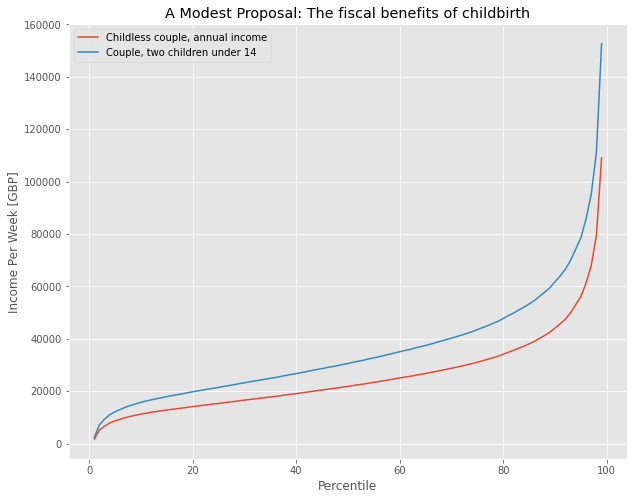
\includegraphics{notebooks/W02. Pandas_files/figure-pdf/cell-18-output-2.png}

}

\end{figure}

\hypertarget{exercise-1}{%
\section{Exercise:}\label{exercise-1}}

Previously, we'd examined income gaps between single people and couples
(how very romantic). Repeat the above exercise (cleaning and plotting
income data) for the columns we used above for single people and
childless couples. Reflect and comment on the differences.

\begin{Shaded}
\begin{Highlighting}[]
\BuiltInTok{print}\NormalTok{(}\StringTok{"Enter your code here"}\NormalTok{)}
\end{Highlighting}
\end{Shaded}

\begin{Shaded}
\begin{Highlighting}[]
\NormalTok{Add your reflection here.}
\end{Highlighting}
\end{Shaded}

So far, we've dealt with selecting data in a particular row of column by
index or label. What if we now want to filter the data by \emph{value}?
For example, let's say I want to see the data for all Childless couples
who earn more than 50,000 (net equivalised) pounds every year. This
looks like:

\begin{Shaded}
\begin{Highlighting}[]
\NormalTok{clean }\OperatorTok{=}\NormalTok{ income[[}\StringTok{\textquotesingle{}Childless couple, annual income\textquotesingle{}}\NormalTok{,}\StringTok{\textquotesingle{}Couple, two children under 14\textquotesingle{}}\NormalTok{]]}
\NormalTok{clean }\OperatorTok{=}\NormalTok{ clean.replace(}\StringTok{\textquotesingle{},\textquotesingle{}}\NormalTok{, }\StringTok{\textquotesingle{}\textquotesingle{}}\NormalTok{, regex}\OperatorTok{=}\VariableTok{True}\NormalTok{)}
\NormalTok{clean }\OperatorTok{=}\NormalTok{ clean.replace(}\StringTok{\textquotesingle{}{-}\textquotesingle{}}\NormalTok{, }\StringTok{\textquotesingle{}NaN\textquotesingle{}}\NormalTok{, regex}\OperatorTok{=}\VariableTok{True}\NormalTok{).astype(}\StringTok{\textquotesingle{}float\textquotesingle{}}\NormalTok{)}
\NormalTok{clean[clean[}\StringTok{\textquotesingle{}Childless couple, annual income\textquotesingle{}}\NormalTok{]}\OperatorTok{\textgreater{}}\DecValTok{50000}\NormalTok{]}
\end{Highlighting}
\end{Shaded}

The key line of code for selection is:

\begin{Shaded}
\begin{Highlighting}[]
\NormalTok{clean[clean[}\StringTok{\textquotesingle{}Childless couple, annual income\textquotesingle{}}\NormalTok{]}\OperatorTok{\textgreater{}}\DecValTok{50000}\NormalTok{]}
\end{Highlighting}
\end{Shaded}

Let's break this down: we're used to using \emph{dataframe}{[}\emph{some
selection}{]} from earlier. Here ``some selection'' is

\begin{Shaded}
\begin{Highlighting}[]
\NormalTok{clean[}\StringTok{\textquotesingle{}Childless couple, annual income\textquotesingle{}}\NormalTok{]}\OperatorTok{\textgreater{}}\DecValTok{50000}
\end{Highlighting}
\end{Shaded}

In other words, this command is returning a set of indices where that
statement is true. We can see this explicitly:

\begin{Shaded}
\begin{Highlighting}[]
\NormalTok{clean[}\StringTok{\textquotesingle{}Childless couple, annual income\textquotesingle{}}\NormalTok{]}\OperatorTok{\textgreater{}}\DecValTok{50000}
\end{Highlighting}
\end{Shaded}

So python is picking the values where this statement is true -
i.e.~where the `Childless couple\ldots{}' column has values greater than
50000. Then this selection is passed to the dataframe, and the dataframe
shows the correct rows.

We won't dwell on comparative operative, here we've used
``\textgreater{}'' to mean ``is greater than''; you can also use:

\begin{itemize}
\tightlist
\item
  == to mean `is equal to' {[}why the double equals?{]}
\item
  \textless\textgreater{} or != to mean `is not equal to'
\item
  \textless{} to mean `is less than'
\item
  the symbol \textgreater= to mean `is greater than or equal to'
\item
  \textless= to mean `is less than or equal to'
\end{itemize}

\hypertarget{exercise-2}{%
\section{Exercise}\label{exercise-2}}

On an approporiately labelled graph, plot the incomes of all single
adults whose net equivalised income is less than or equal to £10,000.
What proportion of the population is this?

\bookmarksetup{startatroot}

\hypertarget{extension-web-scraping}{%
\chapter{Extension: Web Scraping}\label{extension-web-scraping}}

In this example, we've been working with a .csv file that contains all
the data we want. That's not always the case. Let's say we're interested
in getting the data from a table on a website. Websites are built using
HTML code, so what we need to figure out how to look inside the
website's code and pull out the data we want. Luckily, pandas has a
built in function that can automatically recognize HTML tables in
websites and turn them into dataframes.

Let's start with the \href{https://top10.netflix.com/}{Netflix Top 10}
website. Click on the link and have a look around. You'll notice two
tables: the first showing the top 10 films this week, and the second
(farther down) showing the most popular filsms based on their first 28
days on netflix.

We can download both of these tables into python using one pandas
function: read\_html

\begin{Shaded}
\begin{Highlighting}[]
\NormalTok{url}\OperatorTok{=}\StringTok{\textquotesingle{}https://top10.netflix.com/\textquotesingle{}}

\NormalTok{tables}\OperatorTok{=}\NormalTok{pandas.read\_html(url)}

\BuiltInTok{print}\NormalTok{(tables)}
\end{Highlighting}
\end{Shaded}

\begin{verbatim}
[    #  \
0   1   
1   2   
2   3   
3   4   
4   5   
5   6   
6   7   
7   8   
8   9   
9  10   

  .css-ld8rqy-container{position:relative;box-sizing:border-box;min-width:0;}.css-7pg0cj-a11yText{z-index:9999;border:0;clip:rect(1px, 1px, 1px, 1px);height:1px;width:1px;position:absolute;overflow:hidden;padding:0;white-space:nowrap;}.css-3zcu7z-control{-webkit-align-items:center;-webkit-box-align:center;-ms-flex-align:center;align-items:center;background-color:hsl(0, 0%, 100%);border-color:hsl(0, 0%, 80%);border-radius:0;border-style:solid;border-width:1px;box-shadow:none;cursor:pointer;display:-webkit-box;display:-webkit-flex;display:-ms-flexbox;display:flex;-webkit-box-flex-wrap:wrap;-webkit-flex-wrap:wrap;-ms-flex-wrap:wrap;flex-wrap:wrap;-webkit-box-pack:justify;-webkit-justify-content:space-between;justify-content:space-between;min-height:0rem;outline:0!important;position:relative;-webkit-transition:all 100ms;transition:all 100ms;box-sizing:border-box;background:transparent;border:none;padding:0px 3px;margin-left:-5px;}.css-3zcu7z-control:hover{border-color:rgba(255,255,255,0.9);}.css-zl2g27{-webkit-align-items:center;-webkit-box-align:center;-ms-flex-align:center;align-items:center;display:grid;-webkit-flex:1;-ms-flex:1;flex:1;-webkit-box-flex-wrap:wrap;-webkit-flex-wrap:wrap;-ms-flex-wrap:wrap;flex-wrap:wrap;padding:0;-webkit-overflow-scrolling:touch;position:relative;overflow:hidden;box-sizing:border-box;}.css-hlu0h4-singleValue{color:white;grid-area:1/1/2/3;margin-left:2px;margin-right:2px;max-width:100%;overflow:hidden;text-overflow:ellipsis;white-space:nowrap;box-sizing:border-box;}Films (English).css-1a9ai41{margin:0;padding-bottom:2px;padding-top:2px;visibility:visible;color:hsl(0, 0%, 20%);-webkit-flex:1 1 auto;-ms-flex:1 1 auto;flex:1 1 auto;display:inline-grid;grid-area:1/1/2/3;grid-template-columns:0 min-content;box-sizing:border-box;padding:0;}.css-1a9ai41:after{content:attr(data-value) " ";visibility:hidden;white-space:pre;grid-area:1/2;font:inherit;min-width:2px;border:0;margin:0;outline:0;padding:0;}.css-1wy0on6{-webkit-align-items:center;-webkit-box-align:center;-ms-flex-align:center;align-items:center;-webkit-align-self:stretch;-ms-flex-item-align:stretch;align-self:stretch;display:-webkit-box;display:-webkit-flex;display:-ms-flexbox;display:flex;-webkit-flex-shrink:0;-ms-flex-negative:0;flex-shrink:0;box-sizing:border-box;}.css-1hyfx7x{display:none;}.css-xhbtlw-indicatorContainer{color:hsl(0, 0%, 80%);display:-webkit-box;display:-webkit-flex;display:-ms-flexbox;display:flex;padding:8px;-webkit-transition:color 150ms;transition:color 150ms;box-sizing:border-box;-webkit-transform:scale(0.8);-moz-transform:scale(0.8);-ms-transform:scale(0.8);transform:scale(0.8);}.css-xhbtlw-indicatorContainer:hover{color:hsl(0, 0%, 60%);}.css-xhbtlw-indicatorContainer:hover{-webkit-transform:scale(1);-moz-transform:scale(1);-ms-transform:scale(1);transform:scale(1);}  \
0                                Luckiest Girl Alive                                                                                                                                                                                                                                                                                                                                                                                                                                                                                                                                                                                                                                                                                                                                                                                                                                                                                                                                                                                                                                                                                                                                                                                                                                                                                                                                                                                                                                                                                                                                                                                                                                                                                                                                                                                                                                                                                                                                                                                                                                                                                                                                                                                                                                                                                                                                                                                                                                                                                                                                                                                                                                                                                                                                                                                                                                                                                       
1                               Mr. Harrigan's Phone                                                                                                                                                                                                                                                                                                                                                                                                                                                                                                                                                                                                                                                                                                                                                                                                                                                                                                                                                                                                                                                                                                                                                                                                                                                                                                                                                                                                                                                                                                                                                                                                                                                                                                                                                                                                                                                                                                                                                                                                                                                                                                                                                                                                                                                                                                                                                                                                                                                                                                                                                                                                                                                                                                                                                                                                                                                                                       
2                                    Last Seen Alive                                                                                                                                                                                                                                                                                                                                                                                                                                                                                                                                                                                                                                                                                                                                                                                                                                                                                                                                                                                                                                                                                                                                                                                                                                                                                                                                                                                                                                                                                                                                                                                                                                                                                                                                                                                                                                                                                                                                                                                                                                                                                                                                                                                                                                                                                                                                                                                                                                                                                                                                                                                                                                                                                                                                                                                                                                                                                       
3                                             Blonde                                                                                                                                                                                                                                                                                                                                                                                                                                                                                                                                                                                                                                                                                                                                                                                                                                                                                                                                                                                                                                                                                                                                                                                                                                                                                                                                                                                                                                                                                                                                                                                                                                                                                                                                                                                                                                                                                                                                                                                                                                                                                                                                                                                                                                                                                                                                                                                                                                                                                                                                                                                                                                                                                                                                                                                                                                                                                       
4                                                Lou                                                                                                                                                                                                                                                                                                                                                                                                                                                                                                                                                                                                                                                                                                                                                                                                                                                                                                                                                                                                                                                                                                                                                                                                                                                                                                                                                                                                                                                                                                                                                                                                                                                                                                                                                                                                                                                                                                                                                                                                                                                                                                                                                                                                                                                                                                                                                                                                                                                                                                                                                                                                                                                                                                                                                                                                                                                                                       
5                                      The Boss Baby                                                                                                                                                                                                                                                                                                                                                                                                                                                                                                                                                                                                                                                                                                                                                                                                                                                                                                                                                                                                                                                                                                                                                                                                                                                                                                                                                                                                                                                                                                                                                                                                                                                                                                                                                                                                                                                                                                                                                                                                                                                                                                                                                                                                                                                                                                                                                                                                                                                                                                                                                                                                                                                                                                                                                                                                                                                                                       
6                                               Sing                                                                                                                                                                                                                                                                                                                                                                                                                                                                                                                                                                                                                                                                                                                                                                                                                                                                                                                                                                                                                                                                                                                                                                                                                                                                                                                                                                                                                                                                                                                                                                                                                                                                                                                                                                                                                                                                                                                                                                                                                                                                                                                                                                                                                                                                                                                                                                                                                                                                                                                                                                                                                                                                                                                                                                                                                                                                                       
7                                          Marauders                                                                                                                                                                                                                                                                                                                                                                                                                                                                                                                                                                                                                                                                                                                                                                                                                                                                                                                                                                                                                                                                                                                                                                                                                                                                                                                                                                                                                                                                                                                                                                                                                                                                                                                                                                                                                                                                                                                                                                                                                                                                                                                                                                                                                                                                                                                                                                                                                                                                                                                                                                                                                                                                                                                                                                                                                                                                                       
8                                    The Redeem Team                                                                                                                                                                                                                                                                                                                                                                                                                                                                                                                                                                                                                                                                                                                                                                                                                                                                                                                                                                                                                                                                                                                                                                                                                                                                                                                                                                                                                                                                                                                                                                                                                                                                                                                                                                                                                                                                                                                                                                                                                                                                                                                                                                                                                                                                                                                                                                                                                                                                                                                                                                                                                                                                                                                                                                                                                                                                                       
9                            Minions & More Volume 1                                                                                                                                                                                                                                                                                                                                                                                                                                                                                                                                                                                                                                                                                                                                                                                                                                                                                                                                                                                                                                                                                                                                                                                                                                                                                                                                                                                                                                                                                                                                                                                                                                                                                                                                                                                                                                                                                                                                                                                                                                                                                                                                                                                                                                                                                                                                                                                                                                                                                                                                                                                                                                                                                                                                                                                                                                                                                       

   Weeks in Top 10  Hours viewed  
0                1      43080000  
1                1      35420000  
2                2      18810000  
3                2      17410000  
4                3      12600000  
5                1       8510000  
6                1       8420000  
7                2       8350000  
8                1       7850000  
9                3       7090000  ,     #  \
0   1   
1   2   
2   3   
3   4   
4   5   
5   6   
6   7   
7   8   
8   9   
9  10   

  .css-ld8rqy-container{position:relative;box-sizing:border-box;min-width:0;}.css-7pg0cj-a11yText{z-index:9999;border:0;clip:rect(1px, 1px, 1px, 1px);height:1px;width:1px;position:absolute;overflow:hidden;padding:0;white-space:nowrap;}.css-3zcu7z-control{-webkit-align-items:center;-webkit-box-align:center;-ms-flex-align:center;align-items:center;background-color:hsl(0, 0%, 100%);border-color:hsl(0, 0%, 80%);border-radius:0;border-style:solid;border-width:1px;box-shadow:none;cursor:pointer;display:-webkit-box;display:-webkit-flex;display:-ms-flexbox;display:flex;-webkit-box-flex-wrap:wrap;-webkit-flex-wrap:wrap;-ms-flex-wrap:wrap;flex-wrap:wrap;-webkit-box-pack:justify;-webkit-justify-content:space-between;justify-content:space-between;min-height:0rem;outline:0!important;position:relative;-webkit-transition:all 100ms;transition:all 100ms;box-sizing:border-box;background:transparent;border:none;padding:0px 3px;margin-left:-5px;}.css-3zcu7z-control:hover{border-color:rgba(255,255,255,0.9);}.css-zl2g27{-webkit-align-items:center;-webkit-box-align:center;-ms-flex-align:center;align-items:center;display:grid;-webkit-flex:1;-ms-flex:1;flex:1;-webkit-box-flex-wrap:wrap;-webkit-flex-wrap:wrap;-ms-flex-wrap:wrap;flex-wrap:wrap;padding:0;-webkit-overflow-scrolling:touch;position:relative;overflow:hidden;box-sizing:border-box;}.css-hlu0h4-singleValue{color:white;grid-area:1/1/2/3;margin-left:2px;margin-right:2px;max-width:100%;overflow:hidden;text-overflow:ellipsis;white-space:nowrap;box-sizing:border-box;}Films (English).css-1a9ai41{margin:0;padding-bottom:2px;padding-top:2px;visibility:visible;color:hsl(0, 0%, 20%);-webkit-flex:1 1 auto;-ms-flex:1 1 auto;flex:1 1 auto;display:inline-grid;grid-area:1/1/2/3;grid-template-columns:0 min-content;box-sizing:border-box;padding:0;}.css-1a9ai41:after{content:attr(data-value) " ";visibility:hidden;white-space:pre;grid-area:1/2;font:inherit;min-width:2px;border:0;margin:0;outline:0;padding:0;}.css-1wy0on6{-webkit-align-items:center;-webkit-box-align:center;-ms-flex-align:center;align-items:center;-webkit-align-self:stretch;-ms-flex-item-align:stretch;align-self:stretch;display:-webkit-box;display:-webkit-flex;display:-ms-flexbox;display:flex;-webkit-flex-shrink:0;-ms-flex-negative:0;flex-shrink:0;box-sizing:border-box;}.css-1hyfx7x{display:none;}.css-xhbtlw-indicatorContainer{color:hsl(0, 0%, 80%);display:-webkit-box;display:-webkit-flex;display:-ms-flexbox;display:flex;padding:8px;-webkit-transition:color 150ms;transition:color 150ms;box-sizing:border-box;-webkit-transform:scale(0.8);-moz-transform:scale(0.8);-ms-transform:scale(0.8);transform:scale(0.8);}.css-xhbtlw-indicatorContainer:hover{color:hsl(0, 0%, 60%);}.css-xhbtlw-indicatorContainer:hover{-webkit-transform:scale(1);-moz-transform:scale(1);-ms-transform:scale(1);transform:scale(1);}  \
0                                         Red Notice                                                                                                                                                                                                                                                                                                                                                                                                                                                                                                                                                                                                                                                                                                                                                                                                                                                                                                                                                                                                                                                                                                                                                                                                                                                                                                                                                                                                                                                                                                                                                                                                                                                                                                                                                                                                                                                                                                                                                                                                                                                                                                                                                                                                                                                                                                                                                                                                                                                                                                                                                                                                                                                                                                                                                                                                                                                                                       
1                                      Don't Look Up                                                                                                                                                                                                                                                                                                                                                                                                                                                                                                                                                                                                                                                                                                                                                                                                                                                                                                                                                                                                                                                                                                                                                                                                                                                                                                                                                                                                                                                                                                                                                                                                                                                                                                                                                                                                                                                                                                                                                                                                                                                                                                                                                                                                                                                                                                                                                                                                                                                                                                                                                                                                                                                                                                                                                                                                                                                                                       
2                                           Bird Box                                                                                                                                                                                                                                                                                                                                                                                                                                                                                                                                                                                                                                                                                                                                                                                                                                                                                                                                                                                                                                                                                                                                                                                                                                                                                                                                                                                                                                                                                                                                                                                                                                                                                                                                                                                                                                                                                                                                                                                                                                                                                                                                                                                                                                                                                                                                                                                                                                                                                                                                                                                                                                                                                                                                                                                                                                                                                       
3                                       The Gray Man                                                                                                                                                                                                                                                                                                                                                                                                                                                                                                                                                                                                                                                                                                                                                                                                                                                                                                                                                                                                                                                                                                                                                                                                                                                                                                                                                                                                                                                                                                                                                                                                                                                                                                                                                                                                                                                                                                                                                                                                                                                                                                                                                                                                                                                                                                                                                                                                                                                                                                                                                                                                                                                                                                                                                                                                                                                                                       
4                                   The Adam Project                                                                                                                                                                                                                                                                                                                                                                                                                                                                                                                                                                                                                                                                                                                                                                                                                                                                                                                                                                                                                                                                                                                                                                                                                                                                                                                                                                                                                                                                                                                                                                                                                                                                                                                                                                                                                                                                                                                                                                                                                                                                                                                                                                                                                                                                                                                                                                                                                                                                                                                                                                                                                                                                                                                                                                                                                                                                                       
5                                         Extraction                                                                                                                                                                                                                                                                                                                                                                                                                                                                                                                                                                                                                                                                                                                                                                                                                                                                                                                                                                                                                                                                                                                                                                                                                                                                                                                                                                                                                                                                                                                                                                                                                                                                                                                                                                                                                                                                                                                                                                                                                                                                                                                                                                                                                                                                                                                                                                                                                                                                                                                                                                                                                                                                                                                                                                                                                                                                                       
6                                      Purple Hearts                                                                                                                                                                                                                                                                                                                                                                                                                                                                                                                                                                                                                                                                                                                                                                                                                                                                                                                                                                                                                                                                                                                                                                                                                                                                                                                                                                                                                                                                                                                                                                                                                                                                                                                                                                                                                                                                                                                                                                                                                                                                                                                                                                                                                                                                                                                                                                                                                                                                                                                                                                                                                                                                                                                                                                                                                                                                                       
7                                   The Unforgivable                                                                                                                                                                                                                                                                                                                                                                                                                                                                                                                                                                                                                                                                                                                                                                                                                                                                                                                                                                                                                                                                                                                                                                                                                                                                                                                                                                                                                                                                                                                                                                                                                                                                                                                                                                                                                                                                                                                                                                                                                                                                                                                                                                                                                                                                                                                                                                                                                                                                                                                                                                                                                                                                                                                                                                                                                                                                                       
8                                       The Irishman                                                                                                                                                                                                                                                                                                                                                                                                                                                                                                                                                                                                                                                                                                                                                                                                                                                                                                                                                                                                                                                                                                                                                                                                                                                                                                                                                                                                                                                                                                                                                                                                                                                                                                                                                                                                                                                                                                                                                                                                                                                                                                                                                                                                                                                                                                                                                                                                                                                                                                                                                                                                                                                                                                                                                                                                                                                                                       
9                                The Kissing Booth 2                                                                                                                                                                                                                                                                                                                                                                                                                                                                                                                                                                                                                                                                                                                                                                                                                                                                                                                                                                                                                                                                                                                                                                                                                                                                                                                                                                                                                                                                                                                                                                                                                                                                                                                                                                                                                                                                                                                                                                                                                                                                                                                                                                                                                                                                                                                                                                                                                                                                                                                                                                                                                                                                                                                                                                                                                                                                                       

   Hours viewed in first 28 days  
0                      364020000  
1                      359790000  
2                      282020000  
3                      253870000  
4                      233160000  
5                      231340000  
6                      228690000  
7                      214700000  
8                      214570000  
9                      209250000  ]
\end{verbatim}

When we print the results of what was scraped, it's pretty ugly. One of
the reasons is that the \texttt{tables} variable is actually a
\emph{list} of dataframes. Because there were two tables on our website,
\texttt{read\_html} has returned both of those tables and put them in a
list. let's save the first table as a new dataframe called
\texttt{top10} and have a closer look.

\begin{Shaded}
\begin{Highlighting}[]
\NormalTok{top10}\OperatorTok{=}\NormalTok{tables[}\DecValTok{0}\NormalTok{]}
\NormalTok{top10}
\end{Highlighting}
\end{Shaded}

This looks more like the dataframes we were looking at earlier. There's
a big chunk of text (this is HTML code, the language websites are built
with) where the name of the second column should be. \texttt{read\_html}
is usually pretty smart, and can actually read the column names from the
tables on the website. It seems to have gotten confused for this one
column. If we print the columns from the We can rename that column using
the \texttt{rename} function. Since we know it's the second column, we
can select it with \texttt{top10.columns{[}1{]}}

\begin{Shaded}
\begin{Highlighting}[]
\NormalTok{top10.rename(columns}\OperatorTok{=}\NormalTok{\{top10.columns[}\DecValTok{1}\NormalTok{]: }\StringTok{"Title"}\NormalTok{ \}, inplace }\OperatorTok{=} \VariableTok{True}\NormalTok{)}
\NormalTok{top10}
\end{Highlighting}
\end{Shaded}

And there we have it; a nicely formatted dataframe ready for analysis,
straight from a website.

\hypertarget{exercise-3}{%
\section{Exercise}\label{exercise-3}}

Using the following URL
https://en.wikipedia.org/wiki/List\_of\_Nobel\_laureates\_in\_Chemistry
create a plot of the top 10 countries in terms of nobel laureates.
First, follow the steps below:

\begin{Shaded}
\begin{Highlighting}[]
\CommentTok{\# scrape the table of Nobel Laureates in Chemistry using read\_html. remember, this gives us a LIST of dataframes! lets call this list chem\_tables}

\CommentTok{\# select the first dataframe from this list and call it chem}
\end{Highlighting}
\end{Shaded}

I'll help you out with this next bit. We'll be using the
\texttt{groupby} function in pandas to group our dataframe such that
each row is a country (rather than a person, as it currently is). We do
this by using
\texttt{\textless{}dataframe\textgreater{}.groupby(\textquotesingle{}\textless{}column\ name\textgreater{}\textquotesingle{})}.
Since we're aggregating, we need to tell python how we want it to
aggregate our values. In this case, we just want to count the number of
rows for each country; we can do this using \texttt{.size()}. You can
use many different aggregation functions, e.g.~\texttt{.mean()} if you
wanted to calculate the average of a specific column.

\begin{Shaded}
\begin{Highlighting}[]
\CommentTok{\# here, we\textquotesingle{}re creating a new dataframe called \textquotesingle{}country\textquotesingle{} in which each row is a country, and the values represent the number of nobel laureates. }
\NormalTok{countries}\OperatorTok{=}\NormalTok{chem.groupby(}\StringTok{\textquotesingle{}Country[B]\textquotesingle{}}\NormalTok{).size()}

\CommentTok{\#now let\textquotesingle{}s sort it in descending order}
\NormalTok{countries.sort\_values(ascending}\OperatorTok{=}\VariableTok{False}\NormalTok{)}

\CommentTok{\# finally, plot the top 10 countries }
\end{Highlighting}
\end{Shaded}

\bookmarksetup{startatroot}

\hypertarget{spatiotemporal-data}{%
\chapter{Spatiotemporal Data}\label{spatiotemporal-data}}

\hypertarget{workshop-3-open-in-colab}{%
\section[\emph{Workshop 3} ]{\texorpdfstring{\emph{Workshop 3}
\href{https://colab.research.google.com/github/oballinger/QM2/blob/main/notebooks/W03.\%20Spatial\%20Data.ipynb}{\protect
\includegraphics{https://github.com/oballinger/QM2/blob/main/colab-badge.png?raw=1}}}{Workshop 3 Open In Colab}}\label{workshop-3-open-in-colab}}

Sometimes the data we work with references points on the earth's
surface, unlocking a rich set of analytical possibilities. In today's
workshop, we're going to be exploring the effect of the 2020 California
Wildfires on air quality across the state. We'll be using real air
quality data collected by sensors and combining it with satellite
imagery to show how toxic smoke from wildfires swept over America's
largest state.

\hypertarget{aims-1}{%
\subsection{Aims}\label{aims-1}}

\begin{itemize}
\tightlist
\item
  Understanding spatiotemporal data
\item
  Grouping data in pandas
\item
  Manipulating and plotting geographic data
\end{itemize}

\hypertarget{background}{%
\section{Background}\label{background}}

\includegraphics{https://image.cnbcfm.com/api/v1/image/106695701-1599664926959-gettyimages-1228423382-AFP_8PL8JF.jpeg?v=1599664969}

The \href{https://en.wikipedia.org/wiki/2020_California_wildfires}{2020
California wildfire season} was record-setting. By the end of the year,
9,917 fires had burned more than 4\% of the state's area, making 2020
the largest wildfire season recorded in California's modern history.
California's August Complex fire has been described as the first
``gigafire'', burning over 1 million acres across seven counties, an
area larger than the state of Rhode Island. The fires destroyed over
10,000 structures and cost over \$12.079 billion (2020 USD) in damages,
including over \$10 billion in property damage and \$2.079 billion in
fire suppression costs. The intensity of the fire season has been
attributed to a combination of more than a century of poor forest
management and higher temperatures resulting from climate change.

The fires also had a
\href{https://epic.uchicago.edu/news/pollution-from-californias-2020-wildfires-likely-offset-decades-of-air-quality-gains/}{profound
effect on air quality}: ``Places that are experiencing frequent or more
frequent wildfires are going to experience higher air pollution levels,
not just for a couple of days or weeks, but it could impact the annual
level of exposure,'' said Christa Hasenkopf, director of air quality
programs at the University of Chicago institute. ``It can bump up that
average to unsafe and unhealthy levels that really do have an impact on
people's health. When we think of wildfires, we think of short-term
events --- and hopefully they are --- but they can have long-term
consequences considering your overall air pollution exposure.''

\hypertarget{getting-started}{%
\section{Getting Started}\label{getting-started}}

Let's begin by installing some libraries that we'll be working with
today.

\begin{Shaded}
\begin{Highlighting}[]
\OperatorTok{\%\%}\NormalTok{capture}
\OperatorTok{!}\NormalTok{pip install Basemap}
\OperatorTok{!}\NormalTok{pip install ipyleaflet}
\end{Highlighting}
\end{Shaded}

\hypertarget{importing-libraries}{%
\section{Importing Libraries}\label{importing-libraries}}

The first step in any python script is to import the necessary
libraries:

\begin{Shaded}
\begin{Highlighting}[]
\ImportTok{import}\NormalTok{ pandas }\ImportTok{as}\NormalTok{ pd}
\ImportTok{import}\NormalTok{ matplotlib}
\ImportTok{import}\NormalTok{ matplotlib.pyplot }\ImportTok{as}\NormalTok{ plt}
\ImportTok{import}\NormalTok{ numpy }\ImportTok{as}\NormalTok{ np}
\ImportTok{import}\NormalTok{ pylab}
\ImportTok{from}\NormalTok{ datetime }\ImportTok{import}\NormalTok{ datetime}

\OperatorTok{\%}\NormalTok{matplotlib inline}
\NormalTok{pylab.rcParams[}\StringTok{\textquotesingle{}figure.figsize\textquotesingle{}}\NormalTok{] }\OperatorTok{=}\NormalTok{ (}\DecValTok{10}\NormalTok{, }\DecValTok{8}\NormalTok{)}
\end{Highlighting}
\end{Shaded}

\hypertarget{downloading-data-1}{%
\section{Downloading Data}\label{downloading-data-1}}

The next step is to import the data that we need for our analysis. This
week we'll be using real data collected in 2020 by the
\href{https://www.epa.gov/outdoor-air-quality-data/download-daily-data}{Environmental
Protection Agency (EPA)}. I've generated a .csv file containing the data
that I want using the dropdown menus. The EPA also has an
\href{https://aqs.epa.gov/aqsweb/documents/data_api.html}{Application
Programming Interface} for air quality data, which you could use to pull
in data directly into python without having to download a .csv!

\begin{Shaded}
\begin{Highlighting}[]
\OperatorTok{!}\NormalTok{mkdir data}
\OperatorTok{!}\NormalTok{mkdir data}\OperatorTok{/}\NormalTok{wk3}
\OperatorTok{!}\NormalTok{curl https:}\OperatorTok{//}\NormalTok{qm2.s3.eu}\OperatorTok{{-}}\NormalTok{west}\OperatorTok{{-}}\FloatTok{2.}\ErrorTok{amazonaws}\NormalTok{.com}\OperatorTok{/}\NormalTok{wk3}\OperatorTok{/}\NormalTok{california\_aqi.csv }\OperatorTok{{-}}\NormalTok{o .}\OperatorTok{/}\NormalTok{data}\OperatorTok{/}\NormalTok{wk3}\OperatorTok{/}\NormalTok{california\_aqi.csv}
\end{Highlighting}
\end{Shaded}

\begin{verbatim}
  % Total    % Received % Xferd  Average Speed   Time    Time     Time  Current
                                 Dload  Upload   Total   Spent    Left  Speed
100 5586k  100 5586k    0     0  4476k      0  0:00:01  0:00:01 --:--:-- 4479k
\end{verbatim}

Let's open the .csv file and have a look at it:

\begin{Shaded}
\begin{Highlighting}[]
\NormalTok{df}\OperatorTok{=}\NormalTok{pd.read\_csv(}\StringTok{\textquotesingle{}data/wk3/california\_aqi.csv\textquotesingle{}}\NormalTok{)}
\NormalTok{df}
\end{Highlighting}
\end{Shaded}

\begin{longtable}[]{@{}lllllllllll@{}}
\toprule()
& Date & Site ID & POC & PM & AQI & Site Name & CBSA\_NAME & COUNTY &
latitude & longitude \\
\midrule()
\endhead
0 & 1/1/20 & 60010007 & 3 & 8.6 & 36 & Livermore & San
Francisco-Oakland-Hayward, CA & Alameda & 37.687526 & -121.784217 \\
1 & 1/2/20 & 60010007 & 3 & 4.5 & 19 & Livermore & San
Francisco-Oakland-Hayward, CA & Alameda & 37.687526 & -121.784217 \\
2 & 1/3/20 & 60010007 & 3 & 14.2 & 55 & Livermore & San
Francisco-Oakland-Hayward, CA & Alameda & 37.687526 & -121.784217 \\
3 & 1/4/20 & 60010007 & 3 & 10.9 & 45 & Livermore & San
Francisco-Oakland-Hayward, CA & Alameda & 37.687526 & -121.784217 \\
4 & 1/5/20 & 60010007 & 3 & 7.8 & 33 & Livermore & San
Francisco-Oakland-Hayward, CA & Alameda & 37.687526 & -121.784217 \\
... & ... & ... & ... & ... & ... & ... & ... & ... & ... & ... \\
55686 & 11/29/20 & 61131003 & 1 & 20.3 & 68 & Woodland-Gibson Road &
Sacramento-\/-Roseville-\/-Arden-Arcade, CA & Yolo & 38.661210 &
-121.732690 \\
55687 & 12/18/20 & 61131003 & 1 & 2.8 & 12 & Woodland-Gibson Road &
Sacramento-\/-Roseville-\/-Arden-Arcade, CA & Yolo & 38.661210 &
-121.732690 \\
55688 & 12/20/20 & 61131003 & 1 & 22.4 & 73 & Woodland-Gibson Road &
Sacramento-\/-Roseville-\/-Arden-Arcade, CA & Yolo & 38.661210 &
-121.732690 \\
55689 & 12/23/20 & 61131003 & 1 & 11.8 & 49 & Woodland-Gibson Road &
Sacramento-\/-Roseville-\/-Arden-Arcade, CA & Yolo & 38.661210 &
-121.732690 \\
55690 & 12/29/20 & 61131003 & 1 & 5.6 & 23 & Woodland-Gibson Road &
Sacramento-\/-Roseville-\/-Arden-Arcade, CA & Yolo & 38.661210 &
-121.732690 \\
\bottomrule()
\end{longtable}

Each row in this dataset is an individual reading from an air quality
sensor. The first row is a reading from sensor number 60010007 on
January 1st 2020. It is located in Alameda County, and recorded an Air
Quality Index (AQI) reading of 36. So for each sensor (uniquely
identified by the Site ID column) we will have 365 readings. We also
have the latitude and longitude of each one of these air quality
sensors. The presence of these fields makes this
\textbf{spatio-temporal} data. We'll first analyze the temporal
dimension of our data, before adding in the spatial dimension

\hypertarget{temporal-data}{%
\section{Temporal Data}\label{temporal-data}}

Before we go any further, we need to focus on a very special column in
our dataset: the ``Date'' column. We'll be relying heavily on this
dimension of our dataset. Whenever we have temporal data, the first
thing we want to do is check whether pandas is storing it as datetime
information or as a string (text). We can do this using the
\texttt{dtype} function.

\begin{Shaded}
\begin{Highlighting}[]
\BuiltInTok{print}\NormalTok{(}\StringTok{\textquotesingle{}Prior to cleaning, the data type of the "Date" column is:\textquotesingle{}}\NormalTok{, df[}\StringTok{\textquotesingle{}Date\textquotesingle{}}\NormalTok{].dtype)}

\NormalTok{df[}\StringTok{\textquotesingle{}Date\textquotesingle{}}\NormalTok{]}\OperatorTok{=}\NormalTok{pd.to\_datetime(df[}\StringTok{\textquotesingle{}Date\textquotesingle{}}\NormalTok{])}

\BuiltInTok{print}\NormalTok{(}\StringTok{\textquotesingle{}Now, it is stored as: \textquotesingle{}}\NormalTok{, df[}\StringTok{\textquotesingle{}Date\textquotesingle{}}\NormalTok{].dtype)}
\end{Highlighting}
\end{Shaded}

\begin{verbatim}
Prior to cleaning, the data type of the "Date" column is: object
Now, it is stored as:  datetime64[ns]
\end{verbatim}

Once we've stored the Date column as datetime information, we can do all
sorts of useful things with it. For example, we can quickly extract the
month from the date, or even the ``day of year'' (i.e., how many days
since January 1st of that year have passed). Try doing that in one line
of code if your ``Date'' column is stored as text!

\begin{Shaded}
\begin{Highlighting}[]
\CommentTok{\# we can extract the month from the Date column and save it as a new column }
\NormalTok{df[}\StringTok{\textquotesingle{}Month\textquotesingle{}}\NormalTok{]}\OperatorTok{=}\NormalTok{df[}\StringTok{\textquotesingle{}Date\textquotesingle{}}\NormalTok{].dt.month}
\CommentTok{\# we can do the same for the day of year. }
\NormalTok{df[}\StringTok{\textquotesingle{}Day\textquotesingle{}}\NormalTok{]}\OperatorTok{=}\NormalTok{df[}\StringTok{\textquotesingle{}Date\textquotesingle{}}\NormalTok{].dt.dayofyear}

\BuiltInTok{print}\NormalTok{(df[[}\StringTok{\textquotesingle{}Date\textquotesingle{}}\NormalTok{,}\StringTok{\textquotesingle{}Month\textquotesingle{}}\NormalTok{,}\StringTok{\textquotesingle{}Day\textquotesingle{}}\NormalTok{]])}
\end{Highlighting}
\end{Shaded}

\begin{verbatim}
            Date  Month  Day
0     2020-01-01      1    1
1     2020-01-02      1    2
2     2020-01-03      1    3
3     2020-01-04      1    4
4     2020-01-05      1    5
...          ...    ...  ...
55686 2020-11-29     11  334
55687 2020-12-18     12  353
55688 2020-12-20     12  355
55689 2020-12-23     12  358
55690 2020-12-29     12  364

[55691 rows x 3 columns]
\end{verbatim}

When I print the new columns we've made (``Month'' and ``Day'') next to
the original ``Date'' column, we can see that everything is working as
it should. First date (January 1st, 2020), has a value of 1 in the month
column, and a 1 in the day column. The last row in the dataset was a
sensor reading raken on December 29th, 2020. It has a month of 12, and
day-of-year value of 364. Great.

\hypertarget{exercise-4}{%
\subsection{Exercise}\label{exercise-4}}

\href{https://pandas.pydata.org/docs/reference/api/pandas.Series.dt.dayofyear.html}{Here's}
the documentation for the pandas function that allowed us to extract the
day of year from the datetime column. Using the documentation on this
page, create a new column in the dataframe that contains the week of
year.

\hypertarget{grouping-data}{%
\subsection{Grouping Data}\label{grouping-data}}

We can now use the new temporal columns we've created to analyze our
data further. The broadest possible question we're interested in today
is ``What was the effect of the 2020 wildfires on air quality in
California?'' This involves looking at air quality over time, and
comparing pre/post wildfire air quality reading.

To translate that into python, we effectively want to calculate the
average AQI value for all of the sensors in California each day. We can
accomplish this using the \texttt{.groupby()} function in pandas.
\href{https://pandas.pydata.org/docs/reference/api/pandas.DataFrame.groupby.html}{Here}
is the documentation page for the function, give it a quick read.

Remember, each row in our dataframe \texttt{df} is an individual sensor
reading on a given day. We now want a dataframe in which each row is
\emph{one day}, representing the average of \emph{all AQI sensors}. We
can accomplish that using the following line of code, which has four
parts:

\texttt{df.groupby(\textquotesingle{}Day\textquotesingle{}){[}\textquotesingle{}AQI\textquotesingle{}{]}.mean()}

\begin{enumerate}
\def\labelenumi{\arabic{enumi}.}
\tightlist
\item
  \texttt{df}: the dataframe we want to use
\item
  \texttt{.groupby(\textquotesingle{}Day\textquotesingle{})}: the
  groupby function, and the name of the column that we want to group our
  data by. In this case, we want each row in our new dataset to be one
  day, so we're using the ``Day'' column.
\item
  \texttt{{[}\textquotesingle{}AQI\textquotesingle{}{]}}: the data that
  we want to aggregate. Remember, our dataframe has many columns, but we
  want to calculate the average daily value of AQI.
\item
  \texttt{.mean()}: the method of aggregation. We're calculating the
  average in this case, but we could also want to take the maximum value
  (\texttt{.max()}), minimum value (\texttt{.min()}), median
  (\texttt{.median()}), etc.
\end{enumerate}

Let's look at the output from the line of code above. Remember, whenever
we make something new, we must store it somewhere or it disappears! I'm
storing this as a new dataframe called ``daily''.

\begin{Shaded}
\begin{Highlighting}[]
\NormalTok{daily}\OperatorTok{=}\NormalTok{df.groupby(}\StringTok{\textquotesingle{}Day\textquotesingle{}}\NormalTok{)[}\StringTok{\textquotesingle{}AQI\textquotesingle{}}\NormalTok{].mean()}
\NormalTok{daily}
\end{Highlighting}
\end{Shaded}

\begin{verbatim}
Day
1      50.255682
2      43.300000
3      50.437500
4      47.224299
5      39.240602
         ...    
362    33.500000
363    23.358209
364    30.610256
365    39.492754
366    42.532374
Name: AQI, Length: 366, dtype: float64
\end{verbatim}

Now we can see that our dataframe has 366 rows, one for each day of the
year (2020 was actually a leap year!). Let's plot the daily average of
the AQI sensors, along with a dashed vertical line indicating the day a
State of Emergency was declared (August 18th).

\begin{Shaded}
\begin{Highlighting}[]
\CommentTok{\# plot the daily data}
\NormalTok{daily.plot(color}\OperatorTok{=}\StringTok{\textquotesingle{}red\textquotesingle{}}\NormalTok{)}

\CommentTok{\#add title and axis labels}
\NormalTok{plt.title(}\StringTok{\textquotesingle{}Daily Air Quality Index readings in California, 2020\textquotesingle{}}\NormalTok{)}
\NormalTok{plt.ylabel(}\StringTok{\textquotesingle{}AQI\textquotesingle{}}\NormalTok{)}
\NormalTok{plt.xlabel(}\StringTok{\textquotesingle{}Day of Year\textquotesingle{}}\NormalTok{)}

\CommentTok{\# add a dashed black line on August 18th (the 231st day of the year)}
\NormalTok{plt.axvline(}\DecValTok{231}\NormalTok{, color}\OperatorTok{=}\StringTok{\textquotesingle{}black\textquotesingle{}}\NormalTok{, linestyle}\OperatorTok{=}\StringTok{\textquotesingle{}{-}{-}\textquotesingle{}}\NormalTok{, label}\OperatorTok{=}\StringTok{\textquotesingle{}State of Emergency\textquotesingle{}}\NormalTok{)}
\NormalTok{plt.legend()}
\end{Highlighting}
\end{Shaded}

\begin{verbatim}
<matplotlib.legend.Legend at 0x7f6d0e2ab550>
\end{verbatim}

\begin{figure}[H]

{\centering 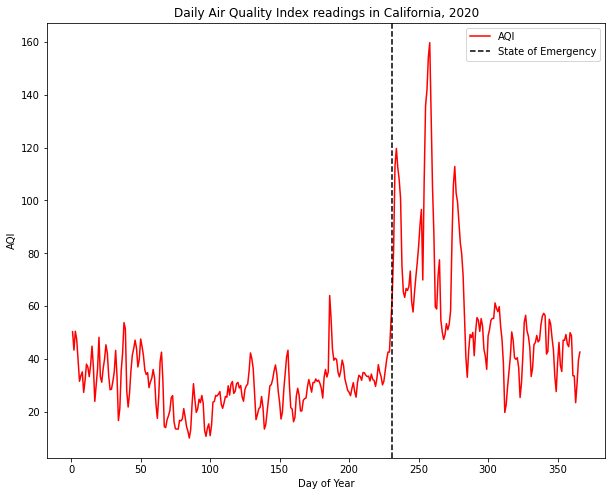
\includegraphics{notebooks/W03. Spatial Data_files/figure-pdf/cell-10-output-2.png}

}

\end{figure}

Pretty cool! We can clearly see some spikes in AQI that correspond
directly to when the state of emergency was declared. Our data is
matching expectations about reality: even though there's no information
about the state of emergency or the wildfires in our dataframe
(remember, it's just a bunch of air quality readings from sensors), we
observe a relationship between our variables (presence of wildfires and
air quality) that conforms to our expectations.

\hypertarget{exercise-5}{%
\subsection{Exercise}\label{exercise-5}}

Now, repeat the above plot but aggregate the dataframe by month rather
than by day. Store the monthly data as a new dataframe called
``monthly''.

\hypertarget{geographic-disparities}{%
\subsection{Geographic Disparities}\label{geographic-disparities}}

OK. We've got a good sense of how the wildfires affected air quality
readings across the whole state. But California is huge; there are
probably geographic disparities in how bad air quality was as a result
of the fires. Let's see which counties were worst affected by the
wildfires.

In our original dataframe, each row was a reading from a given sensor on
a given day. We grouped this data by day to create a dataframe that took
the average of \emph{all} sensors in california for each day as follows:

\texttt{df.groupby(\textquotesingle{}Day\textquotesingle{}){[}\textquotesingle{}AQI\textquotesingle{}{]}.mean()}

Now, we want to plot the average daily air quality by county; this will
involve aggregating both by day \emph{and by county}. Intuitively, we
can accomplish this changing
\texttt{\textquotesingle{}Day\textquotesingle{}} to
\texttt{{[}\textquotesingle{}Day\textquotesingle{},\textquotesingle{}COUNTY\textquotesingle{}{]}},
like so:

\texttt{df.groupby({[}\textquotesingle{}Day\textquotesingle{},\textquotesingle{}COUNTY\textquotesingle{}{]}){[}\textquotesingle{}AQI\textquotesingle{}{]}.mean()}

Let's store this new dataframe and call it ``county\_daily'':

\begin{Shaded}
\begin{Highlighting}[]
\NormalTok{county\_daily}\OperatorTok{=}\NormalTok{df.groupby([}\StringTok{\textquotesingle{}Day\textquotesingle{}}\NormalTok{,}\StringTok{\textquotesingle{}COUNTY\textquotesingle{}}\NormalTok{,])[}\StringTok{\textquotesingle{}AQI\textquotesingle{}}\NormalTok{].mean().reset\_index()}
\NormalTok{county\_daily}
\end{Highlighting}
\end{Shaded}

\begin{longtable}[]{@{}llll@{}}
\toprule()
& Day & COUNTY & AQI \\
\midrule()
\endhead
0 & 1 & Alameda & 44.500000 \\
1 & 1 & Butte & 66.666667 \\
2 & 1 & Calaveras & 63.000000 \\
3 & 1 & Colusa & 78.000000 \\
4 & 1 & Contra Costa & 46.000000 \\
... & ... & ... & ... \\
17314 & 366 & Tehama & 52.000000 \\
17315 & 366 & Trinity & 36.000000 \\
17316 & 366 & Tulare & 62.666667 \\
17317 & 366 & Ventura & 23.666667 \\
17318 & 366 & Yolo & 35.000000 \\
\bottomrule()
\end{longtable}

\hypertarget{exercise-6}{%
\section{Exercise}\label{exercise-6}}

Using the \texttt{groupby} function, create a new dataframe called
``counties'' in which each row is a county, and each value is the
\textbf{maximum} AQI value in that county during the entire year. Then,
sort this dataframe in descending order using
\texttt{.sort\_values(ascending=False)}

Which county had the highest maximum AQI value? Which county had the
lowest? store the names of these counties as varables called ``highest''
and ``lowest'', shown below:

\begin{Shaded}
\begin{Highlighting}[]
\NormalTok{highest}\OperatorTok{=}\StringTok{\textquotesingle{}\textquotesingle{}}
\NormalTok{lowest}\OperatorTok{=}\StringTok{\textquotesingle{}\textquotesingle{}}

\CommentTok{\# Filter the county{-}level daily AQI readings for the worst{-}affected county}
\NormalTok{worst\_county}\OperatorTok{=}\NormalTok{county\_daily[county\_daily[}\StringTok{\textquotesingle{}COUNTY\textquotesingle{}}\NormalTok{]}\OperatorTok{==}\NormalTok{highest]}

\CommentTok{\# Filter the county{-}level daily AQI readings for the least{-}affected county}
\NormalTok{best\_county}\OperatorTok{=}\NormalTok{county\_daily[county\_daily[}\StringTok{\textquotesingle{}COUNTY\textquotesingle{}}\NormalTok{]}\OperatorTok{==}\NormalTok{lowest]}
\end{Highlighting}
\end{Shaded}

Using those two variables, lets plot the AQI values for each of these
counties individually:

\begin{Shaded}
\begin{Highlighting}[]
\CommentTok{\# plot the data from the worst affected county}
\NormalTok{plt.plot(worst\_county[}\StringTok{\textquotesingle{}Day\textquotesingle{}}\NormalTok{], worst\_county[}\StringTok{\textquotesingle{}AQI\textquotesingle{}}\NormalTok{], label}\OperatorTok{=}\NormalTok{highest)}

\CommentTok{\# plot the data from the least affected county}
\NormalTok{plt.plot(best\_county[}\StringTok{\textquotesingle{}Day\textquotesingle{}}\NormalTok{], best\_county[}\StringTok{\textquotesingle{}AQI\textquotesingle{}}\NormalTok{], label}\OperatorTok{=}\NormalTok{lowest)}

\CommentTok{\#add title and axis labels}
\NormalTok{plt.title(}\StringTok{\textquotesingle{}Daily Air Quality Index readings in California, 2020\textquotesingle{}}\NormalTok{)}
\NormalTok{plt.ylabel(}\StringTok{\textquotesingle{}AQI\textquotesingle{}}\NormalTok{)}
\NormalTok{plt.xlabel(}\StringTok{\textquotesingle{}Day of Year\textquotesingle{}}\NormalTok{)}

\CommentTok{\# add a dashed black line on August 18th (the 231st day of the year)}
\NormalTok{plt.axvline(}\DecValTok{231}\NormalTok{, color}\OperatorTok{=}\StringTok{\textquotesingle{}black\textquotesingle{}}\NormalTok{, linestyle}\OperatorTok{=}\StringTok{\textquotesingle{}{-}{-}\textquotesingle{}}\NormalTok{, label}\OperatorTok{=}\StringTok{\textquotesingle{}State of Emergency\textquotesingle{}}\NormalTok{)}
\NormalTok{plt.legend()}
\end{Highlighting}
\end{Shaded}

\begin{verbatim}
<matplotlib.legend.Legend at 0x7f6d0b4f90d0>
\end{verbatim}

\begin{figure}[H]

{\centering 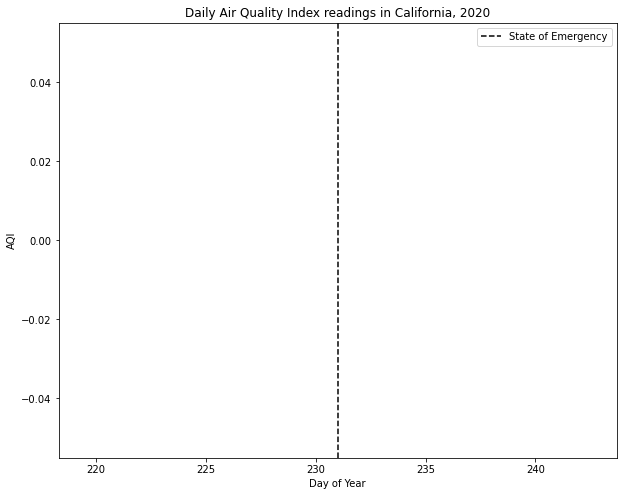
\includegraphics{notebooks/W03. Spatial Data_files/figure-pdf/cell-15-output-2.png}

}

\end{figure}

We can see that the worst affected county suffered a massive spike in
AQI following the wildfires, while the least affected county experienced
a much smaller increase in AQI.

\hypertarget{bringing-in-geography}{%
\section{Bringing in Geography}\label{bringing-in-geography}}

We can explore some limited geographic variation using the ``COUNTY''
column in our dataframe. But we actually have the latitude and longitude
of each individual sensor. We can visualize latitude and longitude data
quite simply as a scatterplot.

Remember, in our original dataframe each row is a reading from a given
sensor on a given day. The sensor's location does not vary over time, so
if we simply plot our original dataframe, we'll have loads of points on
top of each other. Let's pick a specific date, take a slice of our
dataframe on that one date, and plot it. I've picked September 9th based
on the plots above (looks like air quality was really bad).

\begin{Shaded}
\begin{Highlighting}[]
\CommentTok{\# create a variable with the date of interest, September 9th 2020. }
\NormalTok{date}\OperatorTok{=}\StringTok{\textquotesingle{}09{-}09{-}2020\textquotesingle{}}

\CommentTok{\# filter the original dataframe using this date}
\NormalTok{one\_day}\OperatorTok{=}\NormalTok{df[df[}\StringTok{\textquotesingle{}Date\textquotesingle{}}\NormalTok{]}\OperatorTok{==}\NormalTok{date]}

\CommentTok{\# create a scatterplot of sensor locations using latitude and longitude }
\NormalTok{plt.scatter(}
\NormalTok{    x}\OperatorTok{=}\NormalTok{one\_day[}\StringTok{\textquotesingle{}longitude\textquotesingle{}}\NormalTok{],}
\NormalTok{    y}\OperatorTok{=}\NormalTok{one\_day[}\StringTok{\textquotesingle{}latitude\textquotesingle{}}\NormalTok{])}

\CommentTok{\# as always, label our axes and the plot!}
\NormalTok{plt.xlabel(}\StringTok{"Longitude"}\NormalTok{)}
\NormalTok{plt.ylabel(}\StringTok{"Latitude"}\NormalTok{)}
\NormalTok{plt.title(}\StringTok{"Geographic Distribution of AQI sensors in California"}\NormalTok{)}
\end{Highlighting}
\end{Shaded}

\begin{verbatim}
Text(0.5, 1.0, 'Geographic Distribution of AQI sensors in California')
\end{verbatim}

\begin{figure}[H]

{\centering 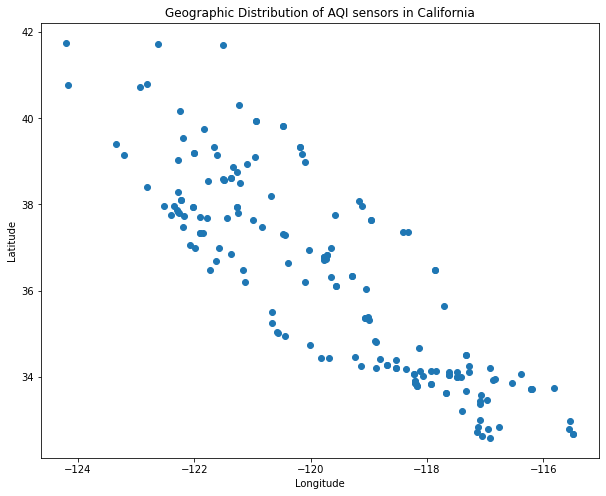
\includegraphics{notebooks/W03. Spatial Data_files/figure-pdf/cell-16-output-2.png}

}

\end{figure}

If you close your eyes and imagine the shape of California, you can
probably see its outline roughly traced in the points above. This plot
leaves a number of things to be desired.

\hypertarget{basemaps}{%
\subsection{Basemaps}\label{basemaps}}

First, we may want to add in a base map of some kind so we can have a
better sense of where each sensor is. For this, we have to import an
extra library called ``Basemap''

\begin{Shaded}
\begin{Highlighting}[]
\CommentTok{\# import Basemap library}
\ImportTok{from}\NormalTok{ mpl\_toolkits.basemap }\ImportTok{import}\NormalTok{ Basemap}

\CommentTok{\# create a basemap, call it \textquotesingle{}map\textquotesingle{}}
\BuiltInTok{map} \OperatorTok{=}\NormalTok{ Basemap(projection}\OperatorTok{=}\StringTok{\textquotesingle{}lcc\textquotesingle{}}\NormalTok{, resolution}\OperatorTok{=}\StringTok{\textquotesingle{}l\textquotesingle{}}\NormalTok{, }\CommentTok{\# this selects the projection of the map.}
\NormalTok{            lat\_0}\OperatorTok{=}\FloatTok{37.5}\NormalTok{, lon\_0}\OperatorTok{={-}}\DecValTok{119}\NormalTok{, }\CommentTok{\# this sets the center of the map }
\NormalTok{            width}\OperatorTok{=}\FloatTok{1E6}\NormalTok{, height}\OperatorTok{=}\FloatTok{1.2E6}\NormalTok{) }\CommentTok{\# this sets the window that we\textquotesingle{}re looking at, in meters.}

\CommentTok{\# We can add features to our blank basemap, including coastlines, as well as state and country boundaries. }
\BuiltInTok{map}\NormalTok{.drawcoastlines(color}\OperatorTok{=}\StringTok{\textquotesingle{}black\textquotesingle{}}\NormalTok{)}
\BuiltInTok{map}\NormalTok{.drawcountries(color}\OperatorTok{=}\StringTok{\textquotesingle{}black\textquotesingle{}}\NormalTok{)}
\BuiltInTok{map}\NormalTok{.drawstates(color}\OperatorTok{=}\StringTok{\textquotesingle{}gray\textquotesingle{}}\NormalTok{)}

\CommentTok{\# Finally, we add in our AQI sensor data on top of the basemap.}
\BuiltInTok{map}\NormalTok{.scatter(}
\NormalTok{    one\_day[}\StringTok{\textquotesingle{}longitude\textquotesingle{}}\NormalTok{], }
\NormalTok{    one\_day[}\StringTok{\textquotesingle{}latitude\textquotesingle{}}\NormalTok{], }
\NormalTok{    latlon}\OperatorTok{=}\VariableTok{True}\NormalTok{)}

\CommentTok{\# as always, title your figure}
\NormalTok{plt.title(}\StringTok{"Geographic Distribution of AQI sensors in California"}\NormalTok{)}
\end{Highlighting}
\end{Shaded}

\begin{verbatim}
Text(0.5, 1.0, 'Geographic Distribution of AQI sensors in California')
\end{verbatim}

\begin{figure}[H]

{\centering 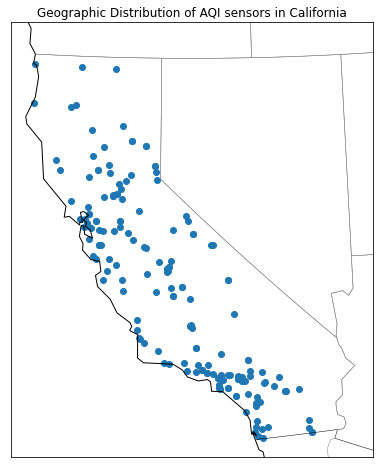
\includegraphics{notebooks/W03. Spatial Data_files/figure-pdf/cell-17-output-2.png}

}

\end{figure}

That's looking a bit better! We now have a much better sense of the
actual distribution of these sensors within california. People who know
the area will recognize clusters of sensors around San Francisco and Los
Angeles; This makes sense, given that these areas have a higher
population density. However, our plot is still missing some pretty
important information: the actual AQI readings!

\hypertarget{colormaps}{%
\subsection{Colormaps}\label{colormaps}}

The whole point of plotting these sensors is to understand the spatial
distribution of air pollution from the 2020 wildfires.

The EPA published the following
\href{https://www.airnow.gov/aqi/aqi-basics/}{table} on their website,
which creates a color-coded scale of AQI values that corresponds to the
impact thereof on human health.

\begin{itemize}
\tightlist
\item
  AQI under 50 is colored green, and indicates ``Good'' air quality.
\item
  AQI between 100 and 200 is generally unhealthy
\item
  AQI over 300 is deemed hazardous.
\end{itemize}

With this in mind, quickly scroll back up to the AQI plots over time. If
you did everything correctly, you should notice that the \emph{average}
AQI value across all sensors in the worst affected county was over 600!

We'll be using the table from the EPA website to build our own color
map. In the code below, I scrape the table and turn it into a
``colormap'' (basically, a dictionary that associates numbers with
colors) that we'll use to color the AQI sensors later.

\begin{Shaded}
\begin{Highlighting}[]
\CommentTok{\# scrape the table of AQI values and corresponding colors }
\CommentTok{\# save it as a dataframe called colors}
\NormalTok{colors}\OperatorTok{=}\NormalTok{pd.read\_html(}\StringTok{\textquotesingle{}https://www.airnow.gov/aqi/aqi{-}basics/\textquotesingle{}}\NormalTok{)[}\DecValTok{0}\NormalTok{]}

\CommentTok{\# create a numerical column for AQI values by splitting the test in the "values of index" column. }
\CommentTok{\# pull out the first string, and convert it to integer}
\NormalTok{colors[}\StringTok{\textquotesingle{}aqi\textquotesingle{}}\NormalTok{]}\OperatorTok{=}\NormalTok{colors[}\StringTok{\textquotesingle{}Values of Index\textquotesingle{}}\NormalTok{].}\BuiltInTok{str}\NormalTok{.split(}\StringTok{\textquotesingle{} \textquotesingle{}}\NormalTok{).}\BuiltInTok{str}\NormalTok{[}\DecValTok{0}\NormalTok{].astype(}\BuiltInTok{int}\NormalTok{)}

\CommentTok{\# print three columns from the dataframe }
\BuiltInTok{print}\NormalTok{(colors[[}\StringTok{\textquotesingle{}aqi\textquotesingle{}}\NormalTok{,}\StringTok{\textquotesingle{}Daily AQI Color\textquotesingle{}}\NormalTok{,}\StringTok{\textquotesingle{}Levels of Concern\textquotesingle{}}\NormalTok{]])}

\CommentTok{\# create a "colormap" from this dataframe using the "Daily AQI Color" column, and the "aqi" column }
\NormalTok{aqi\_colors}\OperatorTok{=}\NormalTok{matplotlib.colors.LinearSegmentedColormap.from\_list(colors[}\StringTok{\textquotesingle{}aqi\textquotesingle{}}\NormalTok{],colors[}\StringTok{\textquotesingle{}Daily AQI Color\textquotesingle{}}\NormalTok{])}
\end{Highlighting}
\end{Shaded}

\begin{verbatim}
   aqi Daily AQI Color               Levels of Concern
0    0           Green                            Good
1   51          Yellow                        Moderate
2  101          Orange  Unhealthy for Sensitive Groups
3  151             Red                       Unhealthy
4  201          Purple                  Very Unhealthy
5  301          Maroon                       Hazardous
\end{verbatim}

Now, we can use this ``aqi\_colors'' object as a color palette later
when we plot the AQI sensors. This way, we will know that green and
yellow points are OK, while red and purple points represent hazardous
levels of air pollution. I've annotated the code above, but it's ok if
you don't get all of it. You could simply load a different colormap in
one line of code; check out the documentation
\href{https://matplotlib.org/stable/tutorials/colors/colormaps.html}{here}.

\begin{Shaded}
\begin{Highlighting}[]
\BuiltInTok{map} \OperatorTok{=}\NormalTok{ Basemap(projection}\OperatorTok{=}\StringTok{\textquotesingle{}lcc\textquotesingle{}}\NormalTok{, resolution}\OperatorTok{=}\StringTok{\textquotesingle{}l\textquotesingle{}}\NormalTok{, }
\NormalTok{            lat\_0}\OperatorTok{=}\FloatTok{37.5}\NormalTok{, lon\_0}\OperatorTok{={-}}\DecValTok{119}\NormalTok{,}
\NormalTok{            width}\OperatorTok{=}\FloatTok{1E6}\NormalTok{, height}\OperatorTok{=}\FloatTok{1.2E6}\NormalTok{)}

\BuiltInTok{map}\NormalTok{.drawcoastlines(color}\OperatorTok{=}\StringTok{\textquotesingle{}black\textquotesingle{}}\NormalTok{)}
\BuiltInTok{map}\NormalTok{.drawcountries(color}\OperatorTok{=}\StringTok{\textquotesingle{}black\textquotesingle{}}\NormalTok{)}
\BuiltInTok{map}\NormalTok{.drawstates(color}\OperatorTok{=}\StringTok{\textquotesingle{}gray\textquotesingle{}}\NormalTok{)}

\BuiltInTok{map}\NormalTok{.scatter(}
\NormalTok{      one\_day[}\StringTok{\textquotesingle{}longitude\textquotesingle{}}\NormalTok{], }
\NormalTok{      one\_day[}\StringTok{\textquotesingle{}latitude\textquotesingle{}}\NormalTok{], }
\NormalTok{      latlon}\OperatorTok{=}\VariableTok{True}\NormalTok{, }
\NormalTok{      c}\OperatorTok{=}\NormalTok{one\_day[}\StringTok{\textquotesingle{}AQI\textquotesingle{}}\NormalTok{], }\CommentTok{\# We\textquotesingle{}re adding that }
\NormalTok{      cmap}\OperatorTok{=}\NormalTok{aqi\_colors, }
\NormalTok{      vmin}\OperatorTok{=}\DecValTok{0}\NormalTok{, }
\NormalTok{      vmax}\OperatorTok{=}\DecValTok{300}\NormalTok{)}


\NormalTok{plt.title(}\StringTok{\textquotesingle{}Air Quality on September 9th, 2020\textquotesingle{}}\NormalTok{)}
\NormalTok{plt.colorbar(label}\OperatorTok{=}\StringTok{\textquotesingle{}Air Quality Index\textquotesingle{}}\NormalTok{)}\OperatorTok{;}
\end{Highlighting}
\end{Shaded}

\begin{figure}[H]

{\centering 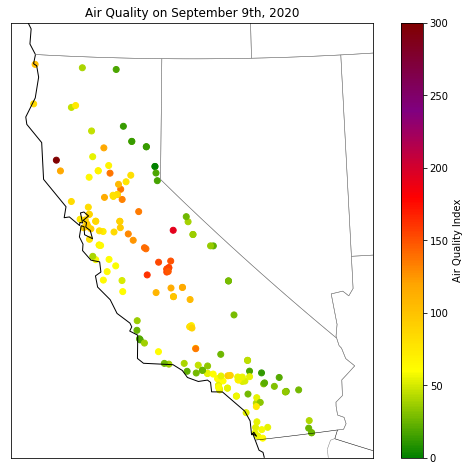
\includegraphics{notebooks/W03. Spatial Data_files/figure-pdf/cell-19-output-1.png}

}

\end{figure}

This plot gives us a good sense of which areas were worst affected by
the wildfires on September 9th, 2020. Areas in the central valley
suffered particularly bad air quality, with AQI reaching hazardous
levels in some areas.

\hypertarget{exercise-7}{%
\subsection{Exercise}\label{exercise-7}}

So far, we've been plotting data from one day, using a dataframe we
generated by filtering the date column like so:
\texttt{one\_day=df{[}df{[}\textquotesingle{}Date\textquotesingle{}{]}==\textquotesingle{}09-09-2020\textquotesingle{}{]}}
(date format is day-month-year).

Using the code from the previous cell, generate a plot of AQI on March
2nd, 2020. After that, use the groupby function to generate a plot of
the maximum AQI reading for each sensor and plot it.

If you've followed along this far, well done! we've come a long way from
a spreadsheet full of sensor readings. But we can go even further!

\hypertarget{advanced-satellite-imagery-and-interactivity}{%
\section{Advanced: Satellite Imagery and
Interactivity}\label{advanced-satellite-imagery-and-interactivity}}

The AQI plots we've generated above give us a good sense of where the
worst air pollution was on a given day; but we're still basically
\emph{inferring} the presence of fires. Luckily, we don't have to do
that. The plumes of smoke generated by the fires were so vast that they
were visible from space. There are a variety of satellites that image
the earth each day (some, like GOES-17, take a picture every few
minutes!).

NASA's Moderate Resolution Imaging Spectroradiometer (MODIS) satellites
take a picture of the same spot on earth nearly every day. So far, we've
been looking at September 9th as a particularly bad day for air quality
in California. Let's have a look at a satellite image from that day. A
Python library called ipyleaflet contains some useful functions that let
us pull up an interactive map of satellite imagery.

\begin{Shaded}
\begin{Highlighting}[]
\CommentTok{\# import the map making modules from ipyleaflet}
\ImportTok{from}\NormalTok{ ipyleaflet }\ImportTok{import}\NormalTok{ Map, Marker, basemaps, basemap\_to\_tiles,Circle}

\CommentTok{\# let create an interactive Map object called "satellite\_map"}
\NormalTok{satellite\_map }\OperatorTok{=}\NormalTok{ Map(}
\NormalTok{  basemap}\OperatorTok{=}\NormalTok{basemap\_to\_tiles( }\CommentTok{\#this function lets us pick from a list of basemaps for our interactive map}
\NormalTok{    basemaps.NASAGIBS.ModisTerraTrueColorCR, }\StringTok{"2020{-}09{-}09"} \CommentTok{\# here we\textquotesingle{}re specifying that we want MODIS imagery, and the date that we want it from  }
\NormalTok{  ),}
\NormalTok{  center}\OperatorTok{=}\NormalTok{(}\FloatTok{36.77}\NormalTok{, }\OperatorTok{{-}}\FloatTok{119.41}\NormalTok{), }\CommentTok{\# then, we want to center the map on california. these coordinates do that}
\NormalTok{  zoom}\OperatorTok{=}\DecValTok{5}\NormalTok{, }\CommentTok{\#finally, we want to set the zoom level of the map. }
\NormalTok{)}

\CommentTok{\# once we\textquotesingle{}ve created the map object we can make it bigger or smaller. let\textquotesingle{}s make it 700 pixels tall. }
\NormalTok{satellite\_map.layout.height }\OperatorTok{=} \StringTok{\textquotesingle{}700px\textquotesingle{}}

\CommentTok{\# now, we visualize it.}
\NormalTok{satellite\_map}
\end{Highlighting}
\end{Shaded}

\begin{verbatim}
Map(center=[36.77, -119.41], controls=(ZoomControl(options=['position', 'zoom_in_text', 'zoom_in_title', 'zoom…
\end{verbatim}

This is a pretty striking image of the West Coast of the U.S. We can see
fluffy white clouds to the East and West, but in the center of the map
plumes of brown smoke emanate from wildfires in California and Oregon.
Use the + - keys in the top left to zoom in, see if you can spot some
wildfires.

\hypertarget{exercise-8}{%
\subsection{Exercise}\label{exercise-8}}

Try changing the code in the cell above to display an image from
September 15th. You could even try importing a different basemap (like
nighttime lights) using this
\href{https://ipyleaflet.readthedocs.io/en/latest/map_and_basemaps/basemaps.html}{list
of basemaps}.

\hypertarget{combining-sensors-and-satellite-images}{%
\section{Combining sensors and satellite
images}\label{combining-sensors-and-satellite-images}}

A cool part of working with spatial data is that we can combine two
completeley different datasets using spatial information. We can add the
AQI sensor data as points to this map.

\begin{Shaded}
\begin{Highlighting}[]
\CommentTok{\# grab the first row from our September 9th dataframe}
\NormalTok{row}\OperatorTok{=}\NormalTok{one\_day.iloc[}\DecValTok{0}\NormalTok{]}
\BuiltInTok{print}\NormalTok{(row)}

\CommentTok{\# This part uses the AQI value in this row (72), and looks up the corresponding color in the colormap we created earlier }
\NormalTok{color}\OperatorTok{=}\NormalTok{matplotlib.colors.rgb2hex(aqi\_colors(row[}\StringTok{\textquotesingle{}AQI\textquotesingle{}}\NormalTok{]))}

\CommentTok{\# Now we create a Circle object using the latitude and longitude from the row, and color it using the color we just selected}
\NormalTok{point}\OperatorTok{=}\NormalTok{Circle(location}\OperatorTok{=}\NormalTok{(row[}\StringTok{\textquotesingle{}latitude\textquotesingle{}}\NormalTok{],row[}\StringTok{\textquotesingle{}longitude\textquotesingle{}}\NormalTok{]), color}\OperatorTok{=}\NormalTok{color)}

\CommentTok{\# Add this as a layer to the satellite\_map object}
\NormalTok{satellite\_map.add\_layer(point)}

\CommentTok{\# Display the updated map}
\NormalTok{satellite\_map}
\end{Highlighting}
\end{Shaded}

\begin{verbatim}
Date                       2020-09-09 00:00:00
Site ID                               60010007
POC                                          3
PM                                        22.3
AQI                                         72
Site Name                            Livermore
CBSA_NAME    San Francisco-Oakland-Hayward, CA
COUNTY                                 Alameda
latitude                             37.687526
longitude                          -121.784217
Month                                        9
Day                                        253
Name: 249, dtype: object
\end{verbatim}

\begin{verbatim}
Map(center=[36.77, -119.41], controls=(ZoomControl(options=['position', 'zoom_in_text', 'zoom_in_title', 'zoom…
\end{verbatim}

It's a bit hard to see, but we've plotted an AQI sensor! its under the
cloud of smoke in the center of the map. You can zoom in to get a closer
look. looks like AQI was pretty bad at this location.

Having plotted one point, we can now plot all the points on September
9th! to do so, we can use the \texttt{iterrows} function in Pandas
which, suprisingly, lets you iterate over rows in a dataframe. The first
line of code below allows us to iterate over the rows in the
\texttt{one\_day} dataframe. It will then run everything in the indented
block for each row; in other words, for each row, it will:

\begin{enumerate}
\def\labelenumi{\arabic{enumi}.}
\tightlist
\item
  use the row's value in the AQI value to select a color for the point
\item
  create a point object using the latitude and longitude columns
\item
  add that point to the satellite map.
\end{enumerate}

\begin{Shaded}
\begin{Highlighting}[]
\ControlFlowTok{for}\NormalTok{ index, row }\KeywordTok{in}\NormalTok{ one\_day.iterrows():}
\NormalTok{  color}\OperatorTok{=}\NormalTok{matplotlib.colors.rgb2hex(aqi\_colors(row[}\StringTok{\textquotesingle{}AQI\textquotesingle{}}\NormalTok{]))}
\NormalTok{  point}\OperatorTok{=}\NormalTok{Circle(location}\OperatorTok{=}\NormalTok{(row[}\StringTok{\textquotesingle{}latitude\textquotesingle{}}\NormalTok{],row[}\StringTok{\textquotesingle{}longitude\textquotesingle{}}\NormalTok{]), color}\OperatorTok{=}\NormalTok{color)}
\NormalTok{  satellite\_map.add\_layer(point)}

\CommentTok{\# display the map}
\NormalTok{satellite\_map}
\end{Highlighting}
\end{Shaded}

\begin{verbatim}
Map(center=[36.77, -119.41], controls=(ZoomControl(options=['position', 'zoom_in_text', 'zoom_in_title', 'zoom…
\end{verbatim}

Theres a pretty striking trend in this data. If you zoom in, you'll see
that the AQI sensors to the East are all green since they are up-wind
from the fires. A few kilometers downwind of the fires, the AQI sensors
display very high readings. Remember, our AQI data and the satellite
imagery are derived from totally different sources, and are totally
different types of data, but they seem to be telling us the same story.
They actually complement each other in important ways. In our original
plot of the AQI sensors without satellite imagery, we could tell that
there was bad air quality on September 9th, but some sensors were green
and others were red. The satellite image shows us that the variation in
AQI across California on September 9th was due to the direction of the
wind, blowing the smoke from the wildfires westward.

\hypertarget{extension-1}{%
\section{Extension}\label{extension-1}}

Now, to save some hassle we can package all the code we used to generate
this map into one clean function. Because we're effectively just
changing the date, we can configure this function so that we can feed it
a different date, and it will grab a satellite image and filter our
dataframe for values occuring on that day. Then, we can draw a new map
in one line of code.

\begin{Shaded}
\begin{Highlighting}[]
\KeywordTok{def}\NormalTok{ satellite\_plot(date):}
  
\NormalTok{  ymd}\OperatorTok{=}\NormalTok{datetime.strptime(date, }\StringTok{\textquotesingle{}}\SpecialCharTok{\%d}\StringTok{{-}\%m{-}\%Y\textquotesingle{}}\NormalTok{).strftime(}\StringTok{\textquotesingle{}\%Y{-}\%m{-}}\SpecialCharTok{\%d}\StringTok{\textquotesingle{}}\NormalTok{)}

\NormalTok{  satellite\_map }\OperatorTok{=}\NormalTok{ Map(}
\NormalTok{    basemap}\OperatorTok{=}\NormalTok{basemap\_to\_tiles(}
\NormalTok{      basemaps.NASAGIBS.ModisTerraTrueColorCR, ymd}
\NormalTok{    ),}
\NormalTok{    center}\OperatorTok{=}\NormalTok{(}\FloatTok{36.77}\NormalTok{, }\OperatorTok{{-}}\FloatTok{119.41}\NormalTok{),}
\NormalTok{    zoom}\OperatorTok{=}\DecValTok{6}\NormalTok{,}
\NormalTok{  )}

\NormalTok{  satellite\_map.layout.height }\OperatorTok{=} \StringTok{\textquotesingle{}700px\textquotesingle{}}

\NormalTok{  one\_day}\OperatorTok{=}\NormalTok{df[df[}\StringTok{\textquotesingle{}Date\textquotesingle{}}\NormalTok{]}\OperatorTok{==}\NormalTok{date]}

  \ControlFlowTok{for}\NormalTok{ index, row }\KeywordTok{in}\NormalTok{ one\_day.iterrows():}
\NormalTok{    color}\OperatorTok{=}\NormalTok{matplotlib.colors.rgb2hex(aqi\_colors(row[}\StringTok{\textquotesingle{}AQI\textquotesingle{}}\NormalTok{]))}
\NormalTok{    point}\OperatorTok{=}\NormalTok{Circle(location}\OperatorTok{=}\NormalTok{(row[}\StringTok{\textquotesingle{}latitude\textquotesingle{}}\NormalTok{],row[}\StringTok{\textquotesingle{}longitude\textquotesingle{}}\NormalTok{]), color}\OperatorTok{=}\NormalTok{color)}
\NormalTok{    satellite\_map.add\_layer(point)}
  \ControlFlowTok{return}\NormalTok{ satellite\_map}

\end{Highlighting}
\end{Shaded}

Now, we can simply change the date in the function and view both
satellite imagery and AQI sensor data from a given day. Look at this
clear day from February 3rd.

\begin{Shaded}
\begin{Highlighting}[]
\NormalTok{satellite\_plot(}\StringTok{\textquotesingle{}02{-}03{-}2020\textquotesingle{}}\NormalTok{)}
\end{Highlighting}
\end{Shaded}

\begin{verbatim}
Map(center=[36.77, -119.41], controls=(ZoomControl(options=['position', 'zoom_in_text', 'zoom_in_title', 'zoom…
\end{verbatim}

All the AQI sensors are showing green values, indicating generally good
air quality. The satellite image shows a few wispy clouds, but no thick
yellow smoke. Now change the date to September 15th, and see what
happens!

\bookmarksetup{startatroot}

\hypertarget{natural-language-processing}{%
\chapter{Natural Language
Processing}\label{natural-language-processing}}

\hypertarget{workshop-4-open-in-colab}{%
\section[\emph{Workshop 4} ]{\texorpdfstring{\emph{Workshop 4}
\href{https://colab.research.google.com/github/oballinger/QM2/blob/main/notebooks/W04.\%20Natural\%20Language\%20Processing.ipynb}{\protect
\includegraphics{https://github.com/oballinger/QM2/blob/main/colab-badge.png?raw=1}}}{Workshop 4 Open In Colab}}\label{workshop-4-open-in-colab}}

Today we'll be using the \emph{Natural Language Tool Kit} package
\textbf{nltk}, which will allow us to split (clean) text into words,
parts of speech, and sentences, and plot word occurrence and frequency.

\textbf{Aims}

\begin{itemize}
\tightlist
\item
  to work with nltk and some standard corpus texts
\item
  to tokenise by word and sentence
\item
  to plot word occurrence and frequency
\item
  to filter by parts of speech
\end{itemize}

\hypertarget{background-1}{%
\section{Background}\label{background-1}}

Exxon Mobil is the 4th largest oil company in the world. In 1978, an
Exxon scientist named James Black wrote an
\href{https://insideclimatenews.org/documents/james-black-1977-presentation/}{internal
briefing} called ``The Greenhouse Effect'' in which he warned: ``Present
thinking holds that man has a time window of five to ten years before
the need for hard decisions regarding changes in energy strategies might
become critical.''

Rather than acting on this information, Exxon spent the next
\href{https://news.harvard.edu/gazette/story/2021/09/oil-companies-discourage-climate-action-study-says/}{forty
years aggressively funding climate denial}. Recently,
\href{https://www.theguardian.com/environment/2022/may/24/exxon-trial-climate-crimes-fossil-fuels-global-heating}{a
U.S. court ruled} that ExxonMobil must face trial over accusations that
it lied about the climate crisis and covered up the fossil fuel
industry's role in worsening environmental devastation.

\hypertarget{earnings-calls}{%
\subsection{Earnings Calls}\label{earnings-calls}}

Every three months, Exxon conducts an
\href{https://www.investopedia.com/terms/e/earnings-call.asp}{``earnings
call''}; a conference call between the management of a public company,
analysts, investors, and the media to discuss the company's financial
results during a given reporting period, such as a quarter or a fiscal
year.

You can
\href{https://globalmeet.webcasts.com/starthere.jsp?ei=1488251\&tp_key=440e363aaf}{register}
to attend their next one if you want! No worries if you miss it, they
provide
\href{https://corporate.exxonmobil.com/Investors/Investor-relations/Investor-materials-archive\#Quarterlyearningsmaterials}{transcripts}
on their website.

These transcripts provide an intimate window into the company's . We can
see how much pressure investors are putting on the company to tackle
climate change, and how the company responds.

We'll be working with transcripts spanning nealry 20 years and over 10
million words; that's like reading the Harry Potter series 10 times.


\includegraphics{https://haha.business/business.jpg}

\hypertarget{downloading-the-data-1}{%
\section{Downloading the Data}\label{downloading-the-data-1}}

Let's grab the data we will need this week from our course website and
save it into our data folder. If you've not already created a data
folder then do so using the following command.

Don't worry if it generates an error, that means you've already got a
data folder.

\begin{Shaded}
\begin{Highlighting}[]
\OperatorTok{\%\%}\NormalTok{capture}
\OperatorTok{!}\NormalTok{pip install spacy}
\OperatorTok{!}\NormalTok{pip install textacy}
\OperatorTok{!}\NormalTok{pip install nltk}
\OperatorTok{!}\NormalTok{pip install scattertext}
\OperatorTok{!}\NormalTok{pip install tika}
\end{Highlighting}
\end{Shaded}

\begin{Shaded}
\begin{Highlighting}[]
\CommentTok{\#Make a ./data/wk4 directory}
\OperatorTok{!}\NormalTok{mkdir data}\OperatorTok{/}\NormalTok{wk4}

\end{Highlighting}
\end{Shaded}

\begin{verbatim}
mkdir: cannot create directory ‘data/wk4’: File exists
\end{verbatim}

\begin{Shaded}
\begin{Highlighting}[]
\ImportTok{import}\NormalTok{ spacy}
\ImportTok{import}\NormalTok{ json}
\ImportTok{import}\NormalTok{ pylab}
\ImportTok{from}\NormalTok{ IPython.core.display }\ImportTok{import}\NormalTok{ display, HTML}
\ImportTok{import}\NormalTok{ nltk}
\ImportTok{import}\NormalTok{ tika }
\ImportTok{import}\NormalTok{ numpy }\ImportTok{as}\NormalTok{ np}
\ImportTok{import}\NormalTok{ pandas }\ImportTok{as}\NormalTok{ pd}
\ImportTok{import}\NormalTok{ matplotlib.pyplot }\ImportTok{as}\NormalTok{ plt}

\OperatorTok{\%}\NormalTok{matplotlib inline}

\NormalTok{nltk.download(}\StringTok{\textquotesingle{}stopwords\textquotesingle{}}\NormalTok{)}
\NormalTok{pylab.rcParams[}\StringTok{\textquotesingle{}figure.figsize\textquotesingle{}}\NormalTok{] }\OperatorTok{=}\NormalTok{ (}\FloatTok{10.}\NormalTok{, }\FloatTok{8.}\NormalTok{)}
\NormalTok{nlp }\OperatorTok{=}\NormalTok{ spacy.load(}\StringTok{"en\_core\_web\_sm"}\NormalTok{)}
\end{Highlighting}
\end{Shaded}

\begin{verbatim}
[nltk_data] Downloading package stopwords to /root/nltk_data...
[nltk_data]   Package stopwords is already up-to-date!
\end{verbatim}

Exxon host earnings calls on their website in PDF form. Usually, working
with PDFs is a real pain as they are not machine-readable. Using a
python package called
\href{https://www.geeksforgeeks.org/parsing-pdfs-in-python-with-tika/}{tika},
we can ``parse'' a pdf, turning it into machine-readable text:

\begin{Shaded}
\begin{Highlighting}[]
\CommentTok{\# define the URL where your PDF lives. You could also upload your own pdf.}
\NormalTok{url}\OperatorTok{=}\StringTok{\textquotesingle{}https://corporate.exxonmobil.com/{-}/media/Global/Files/investor{-}relations/quarterly{-}earnings/earnings{-}transcripts/2022{-}earnings{-}transcripts/1Q22{-}XOM{-}Earnings{-}Call{-}Transcript{-}4{-}29{-}22.pdf\textquotesingle{}}

\CommentTok{\# parse the pdf by feeding tika the URL and store the text in an object called "raw" }
\NormalTok{raw }\OperatorTok{=}\NormalTok{ parser.from\_file(url)}
\end{Highlighting}
\end{Shaded}

\begin{verbatim}
2022-10-20 12:45:27,036 [MainThread  ] [INFO ]  Retrieving https://corporate.exxonmobil.com/-/media/Global/Files/investor-relations/quarterly-earnings/earnings-transcripts/2022-earnings-transcripts/1Q22-XOM-Earnings-Call-Transcript-4-29-22.pdf to /tmp/media-global-files-investor-relations-quarterly-earnings-earnings-transcripts-2022-earnings-transcripts-1q22-xom-earnings-call-transcript-4-29-22.pdf.
INFO:tika.tika:Retrieving https://corporate.exxonmobil.com/-/media/Global/Files/investor-relations/quarterly-earnings/earnings-transcripts/2022-earnings-transcripts/1Q22-XOM-Earnings-Call-Transcript-4-29-22.pdf to /tmp/media-global-files-investor-relations-quarterly-earnings-earnings-transcripts-2022-earnings-transcripts-1q22-xom-earnings-call-transcript-4-29-22.pdf.
\end{verbatim}

Now, we have an object called ``raw'' that contains some useful
information. Notice the squiggly brackets; this is a dictionary. It
contains several fields, including some useful metadata such as the
author

\begin{Shaded}
\begin{Highlighting}[]
\NormalTok{date}\OperatorTok{=}\NormalTok{raw[}\StringTok{\textquotesingle{}metadata\textquotesingle{}}\NormalTok{][}\StringTok{\textquotesingle{}date\textquotesingle{}}\NormalTok{]}
\NormalTok{title}\OperatorTok{=}\NormalTok{raw[}\StringTok{\textquotesingle{}metadata\textquotesingle{}}\NormalTok{][}\StringTok{\textquotesingle{}dc:title\textquotesingle{}}\NormalTok{]}
\NormalTok{raw\_text}\OperatorTok{=}\NormalTok{raw[}\StringTok{\textquotesingle{}content\textquotesingle{}}\NormalTok{]}

\BuiltInTok{print}\NormalTok{(}\StringTok{\textquotesingle{}Date: \textquotesingle{}}\NormalTok{, date)}
\BuiltInTok{print}\NormalTok{(}\StringTok{\textquotesingle{}Title: \textquotesingle{}}\NormalTok{, title)}
\BuiltInTok{print}\NormalTok{(}\StringTok{\textquotesingle{}Word Count: \textquotesingle{}}\NormalTok{, }\BuiltInTok{len}\NormalTok{(raw\_text))}
\BuiltInTok{print}\NormalTok{(}\StringTok{\textquotesingle{}Text:\textquotesingle{}}\NormalTok{)}
\NormalTok{raw\_text}
\end{Highlighting}
\end{Shaded}

\begin{verbatim}
Date:  2022-05-04T16:51:56Z
Title:  1Q22 XOM Earnings Call Transcript 4-29-22
Word Count:  58778
Text:
\end{verbatim}

\begin{verbatim}
"\n\n\n\n\n\n\n\n\n\n\n\n\n\n\n\n\n\n\n\n\n\n\n\n\n\n\n\n\n\n\n\n\n\n\n\n\n\n\n\n\n\n\n1Q22 XOM Earnings Call Transcript 4-29-22\n\n\n \n \n\n  1  \n\nExxonMobil First Quarter 2022 Earnings Call Transcript \n\nThis transcript presents ExxonMobil’s first quarter 2022 earnings call held on April 29, 2022. \n\n \n\nOperator: Good day, everyone.  Welcome to this ExxonMobil Corporation First Quarter 2022 \n\nEarnings Call.  Today's call is being recorded.  At this time, I'd like to turn the call over to the Vice \n\nPresident of Investor Relations, Mrs. Jennifer Driscoll.  Please go ahead, ma'am.   \n\n \n\nJennifer Driscoll: Good morning, everyone.  Welcome to our first quarter earnings call.  We appreciate \n\nyour interest in ExxonMobil.  Joining me today are Darren Woods, our Chairman, and Chief \n\nExecutive Officer; and Kathy Mikells, our Senior Vice-President, and Chief Financial Officer.   \n\n \n\n The slides and our prerecorded remarks were made available on our Investor Section of our \n\nwebsite earlier this morning along with our news release.  In a minute, Darren will provide \n\nopening comments, and reference a few slides from that presentation.  Then, we'll conduct a \n\nquestion-and-answer session.   \n\n \n\n We expect to conclude the call by about 9:30 AM Central Time.  Let me encourage you to read \n\nour cautionary statement, which is on slide 2.  Please note we also provided supplemental \n\ninformation at the end of our earnings slides, which are posted on the website.  Now, I'll turn the \n\ncall over to Darren Woods.   \n\n \n\nDarren Woods: Good morning, and thanks for joining us today.  As we laid out at our most recent \n\nInvestor Day, our goal is to sustainably grow shareholder value through the execution of our \n\nstrategic priorities as seen on this slide.  As we think about recent events, our job has never been \n\nclearer or more important.   \n\n \n\n The need to meet society's evolving needs reliably and affordably is what consumers and \n\nbusinesses across the globe are demanding, and what we delivered this quarter.  First, we \n\n\n\n \n \n\n  2  \n\ncontinue to build our competitively advantaged production portfolio, bringing new barrels to \n\nmarket today driven in part by the high-value investments.   \n\n \n\n We continue to progress through the pandemic-driven downturn in prices.  A prime example of \n\nthe benefits of our continued investments is Guyana.  This quarter saw the successful start-up of \n\nLiza Phase 2.  Production is ramping up ahead of schedule, and is expected to reach capacity of \n\n220,000 barrels of oil per day by the third quarter this year.   \n\n \n\n Combined with Liza Phase 1, it will bring our total production capacity in Guyana to more than \n\n340,000 barrels per day.  Our third project, Payara, is running ahead of schedule with startup now \n\nlikely by yearend 2023.  Yellowtail, the fourth and largest project to date on the Stabroek block, \n\nreceived government approval of our development plan, and is on schedule to start up in 2025.   \n\n \n\n Further adding to our portfolio, we have made five new discoveries this year that have increased \n\nthe estimated recoverable resources to nearly 11 billion oil-equivalent barrels.  Turning to the US, \n\nwe continue to grow production in the Permian Basin.  In March, we produced about 560,000 oil-\n\nequivalent barrels per day on pace to deliver a 25% increase versus 2021.   \n\n \n\n Looking forward, we are also growing our globally diverse portfolio of low-cost, capital-efficient \n\nLNG developments.  In Mozambique, the 3.4 million-ton-per-year Coral South Floating LNG \n\nproduction vessel is being commissioned after arriving on site in January.  Coral South is on \n\nbudget with the first LNG cargo expected in the fourth quarter.   \n\n \n\n In addition to investing in high-value opportunities in our existing businesses, we are also \n\nadvancing opportunities in our Low Carbon Solutions business.  During the quarter, we \n\nannounced plans to build a large-scale hydrogen plant in Baytown, Texas.  We anticipate the \n\nfacility will have the capacity to produce up to 1 billion cubic feet of hydrogen per day.   \n\n \n\n\n\n \n \n\n  3  \n\n Combined with carbon capture, transport, and storage of approximately 10 million metric tons of \n\nCO2 per year, this facility will be a foundational investment in the development of the Houston \n\nCCS Hub, which will have the potential to eliminate 100 million metric tons of CO2 per year, and \n\nrepresents a meaningful step forward in advancing accretive, low-carbon solutions.   \n\n \n\n We also reached a final investment decision to expand another important carbon capture and \n\nstorage project at our helium plant in Wyoming.  In addition, we received the top certification of \n\nour management of methane emissions at our Poker Lake development in the Permian.   \n\n \n\n We are the first company to achieve this certification for natural gas production associated with \n\noil.  At the end of the first quarter, we implemented a series of organizational changes to further \n\nleverage the scale and integration of the corporation, improve the effectiveness of our operations, \n\nand better serve our customers.   \n\n \n\n We combined our downstream and chemical operations into a single Product Solutions business.  \n\nThis new integrated business will be focused on developing high-value products, improving \n\nportfolio value, and leading in sustainability.  As a result of these changes, our company is now \n\norganized along three primary businesses: Upstream, Product Solutions, and Low Carbon \n\nSolutions.   \n\n \n\n These three businesses are supported by corporate-wide organizations including projects, \n\ntechnology, engineering, operations, safety, and sustainability.  Before I cover our financial \n\nresults, I wanted to provide our perspective on the market environment.  In the first quarter, a tight \n\nsupply/demand environment primarily due to the low investment levels during the pandemic \n\ncontributed to rapid increases in prices for crude, natural gas, and refined products.   \n\n \n\n Clearly, the events in Ukraine have added uncertainty to what was already a tight supply outlook.  \n\nBrent rose by about $22 dollars per barrel or 27% versus the fourth quarter.  Today, natural gas \n\n\n\n \n \n\n  4  \n\nprices remain well above the 10-year historical ranges driven by tight global market conditions \n\nand ongoing European supply concerns.   \n\n \n\n The same tight supply/demand factors have also pushed refining margins near the top of the \n\nrange.  Chemical margins in Asia have fallen sharply with product prices lagging the steep \n\nincreases in feed and energy costs.  In our case, the US ethane feed advantage provided a \n\nsignificant positive offset versus this global view.   \n\n \n\n With that market environment as the backdrop, let me turn to our first quarter financials.  Earnings \n\ntotaled $8.8 billion, excluding an identified item, the after-tax charge associated with Sakhalin-1.  \n\nAs you know, we are discontinuing our Sakhalin-1 operations in Russia, which represented less \n\nthan 2% of our total production last year, about 65,000 oil-equivalent barrels per day, and about \n\n1% of our corporate operating earnings.   \n\n \n\n As the operator, our priority continues to be the health and safety of our people, and the \n\nprotection of the environment.  Of course, we remain in full compliance with all US sanctions, and \n\nare closely coordinating with the US Administration.  Turning to structural savings, we continue to \n\ndrive further efficiencies now delivering more than $5 billon of annual savings versus 2019.   \n\n \n\n Capex totaled $4.9 billion for the quarter in line with our full-year guidance of $21 to $24 billion.  \n\nCash flow from operations was $14.8 billion, maintaining our strong balance sheet.  Our debt-to-\n\ncapital ratio remains near the low end of our 20%-25% target range, while our net debt-to-capital \n\nratio dropped to about 17%.   \n\n \n\n We returned $5.8 billion to shareholders, of which about two-thirds was in the form of dividends \n\nand the remainder share repurchases, consistent with our previous program.  We said during our \n\nCorporate Plan Update in December that we expect to repurchase $10 billion dollars of our \n\nshares.   \n\n\n\n \n \n\n  5  \n\n \n\n This morning we announced an increase to the program, up to $30 billion dollars in total through \n\n2023.  This move reflects the confidence we have in our strategy, the performance we are seeing \n\nacross our businesses, and the strength of our balance sheet.  Before I leave you with a few key \n\ntakeaways, let me share one other decision we made this month with respect to our workforce.   \n\n \n\n Continually investing in our people and maintaining a strong culture are core strategic priorities \n\nand essential to achieving our long-term objectives.  As part of that effort, we are tripling the \n\nnumber of employees eligible for stock grants by bringing in high-performing employees at earlier \n\nstages of their careers.   \n\n \n\n Our goal is to increase our people's ownership in the company, and importantly in our financial \n\nand operating results.  Secondly, in June, we will implement a 3% off-cycle compensation \n\nadjustment in the US to maintain competitiveness.  Our compensation and benefits programs are \n\na key element of our total value proposition that enables us to continue to attract and retain the \n\nbest talent in the industry.   \n\n \n\n Let me leave you with a few key takeaways.  We had a strong first quarter, and I'm proud of the \n\norganization's progress.  The impact of weather on the upstream volumes and derivatives and \n\ntiming impacts in the downstream obscured a strong underlying performance.  We anticipate an \n\nabsence of these impacts and strong refining margins will position us very well in the second \n\nquarter.  We are making outstanding progress on our high-value growth developments in \n\nGuyana, the Permian, and LNG.  Our new Corpus Christi Chemical Complex is up and running \n\nahead of schedule, and generated positive earnings and cash flow in its first quarter of \n\noperations.   \n\n \n\n We have strengthened the balance sheet and are creating value for shareholders through an \n\nattractive dividend and increased share repurchases.  We are advancing hydrogen, biofuels, and \n\n\n\n \n \n\n  6  \n\nother low-carbon solutions consistent with our intention to lead in the energy transition, leveraging \n\nour competitive advantages of scale, integration, and technology.   \n\n \n\n Finally, we are evolving our organization from a holding company to an operating company to \n\nbetter serve our customers' evolving needs and grow long-term shareholder value.  Before we \n\ntake your questions, I want to acknowledge the very real impact the high prices are having on \n\nfamilies all around the world.   \n\n \n\n You may recall that we anticipated this in 2020 with industry investment levels well below those \n\nrequired to offset depletion.  That is why we worked so hard to preserve our capital expenditures \n\nduring the depths of the pandemic and ensure that additional production was available to meet \n\nthe eventual recovery in demand.   \n\n \n\n Today, that long-term focus is paying off with growing production of industry-advantaged supply.  \n\nWe are continuing to focus on the fundamentals through ongoing investment in advantaged \n\nprojects and low-emission initiatives to ensure that we can continue to meet the critical needs of \n\npeople all around the world reliably and affordably well into the future.   \n\n \n\nJennifer Driscoll: Thank you, Darren.  One last piece of housekeeping I wanted to mention is that \n\nahead of the segment reporting change next quarter, we plan to provide you annual and quarterly \n\ninformation for the past five years using the new reporting segments to assist you with your \n\nmodeling.  We plan to post the new data on our website around mid-June.   \n\n \n\n Also, please note that starting with this call, we ask our analysts to limit themselves to a single \n\nquestion.  So, that we can fit in questions for more people.  However, you may remain on the line \n\nin case clarification is needed.  And with that operator, please provide the instructions and then \n\nopen the phone lines for the first question.   \n\n \n\n\n\n \n \n\n  7  \n\nOperator: Thank you, Mrs. Driscoll.  The question-and-answer session will be conducted \n\nelectronically.  If you'd like to ask a question, please do so by pressing the star key followed by \n\nthe digit one on your touchtone telephone.  Once again, we request that you limit yourselves to \n\none question, so, that we may take as many questions as possible.   \n\n \n\n We'll take our first question from the line of Phil Gresh with JP Morgan.   \n\n \n\nPhil Gresh: Yes, hi.  Good morning, Darren and Kathy.   \n\n \n\nDarren Woods: Good morning.   \n\n \n\nPhil Gresh: So, I guess my question is a little bit of a two-part question, then.  The buyback, $30 \n\nbillion over two years, previously you talked about I think $10 billion mostly in 2022.  So, should we \n\nassume the $30 billion is essentially rateable, $15 billion this year?  And then if that's the case, it still \n\nseems like there's a lot of excess cash potentially building up at strip prices.  So, how do you think about \n\nany excess cash, debt reduction, etc. given where the leverage is versus targets now?  Thank you.   \n\n \n\nKathryn Mikells: Great.  Thanks very much.  So, look, we don't know exactly how long the strong \n\nmarket conditions that we're seeing today are going to persist.  And we've learned some pretty \n\ntough liquidity lessons during the pandemic so our cash balance has been building a bit.   \n\n \n\n You would see that it was $11 billion as we ended the quarter.  So, you should expect with the \n\nbackdrop of these strong market conditions that even with the higher buyback program that we \n\nannounced this morning, we would be building our cash in the near term, potentially between $20 \n\nto $30 billion over time.   \n\n \n\n And so, that really addresses our need for flexibility in what's an incredibly uncertain environment.  \n\nand ensuring that we'll continue to appropriately invest in the business and sustain the share \n\n\n\n \n \n\n  8  \n\nrepurchase program that we talked about through 2023.  In terms of just how to think about the \n\npace and the program, it's up to $30 billion through the end of 2023.   \n\n \n\n We obviously got $2.1 billion done in this quarter.  You should think about us looking to get up to \n\na ratable pace.  And that roughly, we'd be looking to get $15 billion done a year.  Again, looking \n\nto sustain the program more consistently over this two-year period.  So, that's how I would think \n\nabout roughly where we see our cash balance, and just looking to maintain a lot of flexibility in \n\nwhat's a pretty uncertain environment.   \n\n \n\n And we did learn some real lessons during the pandemic.  We used to try and hold our cash \n\nbalance, call it between $3 billion and $5 billion, and run a lot of commercial paper.  And when the \n\npandemic hit, that was quite problematic for the company.  So, we're going to be a little bit more \n\nconservative here in the near term.   \n\n \n\nOperator: Your next question comes from the line of Jeanine Wai with Barclays.   \n\n \n\nJeanine Wai: Hi.  Good morning, everyone.  Thanks for taking our questions.   \n\n \n\nDarren Woods: Morning.   \n\n \n\nJeanine Wai: Good morning.  Our question is related broadly to your global gas opportunities.  Can you \n\ntalk about how you see the evolution of the US market?  And how do you see certified gas \n\nplaying a role in US supply?  And I guess, do you intend to really look for a global outlet for a \n\nportion of your US gas?   \n\n \n\n And we understand that Golden Pass, that provides a great opportunity to capture the spread.  \n\nBut maybe, are you thinking about some other opportunities besides Golden Pass?  Thank you.   \n\n \n\n\n\n \n \n\n  9  \n\nDarren Woods: Sure.  You're welcome, Jeanine, and good to hear from you again.  Just maybe a broad \n\ncomment on the LNG business.  Obviously, as we're seeing across each of our sectors, the \n\npandemic had a pretty profound effect with respect to deferring, delaying capital spend, and \n\ntherefore additional capacity coming on.   \n\n \n\n And as the pandemic has subsided and demand has recovered, we're seeing very tight markets.  \n\nAnd we're seeing that play out really around the world, obviously a significant impact.  And then \n\nwith the Ukraine and the situation there, that has added a significant additional level of \n\nuncertainty around supply.   \n\n \n\n And so, I think a very dynamic market and a very high-priced market.  And what we've seen in \n\nresponse to that is basically very full capacity utilization all around the world maximizing the \n\namount of LNG moving.  Obviously, we've got our Coral LNG starting up later this year, which will \n\nhelp contribute to and ease some of that tightness.   \n\n \n\n And then you mentioned Golden Pass, which is an important leg of our strategy of making sure \n\nthat we have access to LNG supplies that we can use to supply demand all around the world.  \n\nAnd that's a very important part of our strategy in LNG going forward is making sure that we've \n\ngot barrels that we can then move and trade in the marketplace, and move across the different \n\nregional demand centers.   \n\n \n\n And so, I think we're going to continue to look for opportunities in LNG.  It's an important part of \n\nthe portfolio.  We've got opportunities in PNG that we're progressing.  Obviously, additional \n\ninvestments in Mozambique are in the future as well.  And so, I think, it'll be a very important \n\nfoundational layer of supply, and a really important part of our overall business offer.   \n\n \n\nKathryn Mikells: And I would just add.  You asked a little bit about that top rating that we got on \n\nmethane management in Poker Lake in the Permian.  And we would say, we really see a market \n\n\n\n \n \n\n  10  \n\nover time building for lower-emission products, and that really plays into that.  And we would \n\ncertainly hope that we'd also start to see a premium on those lower-emission products, right.   \n\n \n\n And we'd say that's consistent across our business, but we definitely are looking to play into that \n\ngoing forward.   \n\n \n\nDarren Woods: Yeah, I would just add to that.  Obviously, that would be a benefit.  But it's certainly not \n\nthe main driver with respect to making sure that our operations have very low emissions, and very \n\nlow methane emissions.  And so, that's a core part of our commitment in running these facilities.   \n\n \n\n And to the extent the market pays a premium for that, that's an advantage that we'll look to take \n\nadvantage of.   \n\n \n\nOperator: Your next question comes from the line of Devin McDermott with Morgan Stanley.   \n\n \n\nDevin McDermott: Hey, good morning.  Thanks for taking my question.   \n\n \n\nDarren Woods: Morning.   \n\n \n\nDevin McDermott: I wanted to ask about some of the structural cost reduction goals.  You continue to \n\nmake good progress there.  But the question is, can you add a little bit of color around what \n\nyou're seeing on just broad cost in inflation, labor, and otherwise?  And how if at all that impacts \n\nsome of those goals and targets over time?   \n\n \n\nKathryn Mikells: Sure.  So, I'll start out with just saying, we feel good about the progress that we're \n\ncontinuing to make.  At the end of the fourth quarter, we had said we had gotten to about $5 \n\nbillion in structural cost savings relative to 2019 we are now at $5.4 billion so I'd say overall, we \n\nfeel really good about that progress.   \n\n\n\n \n \n\n  11  \n\n \n\n Obviously, we have now put in place the new organizational structure, which should drive \n\nincremental efficiencies on top of just driving better operations, faster speed-to-market, better \n\ndeployment, faster deployment of resources to the highest opportunities across the company.   \n\n \n\n We're not immune to inflation obviously and we would see a fair amount of both energy and \n\nfeedstock inflation coming through the business in certain areas that put a little bit of pressure on \n\nmargins.  Overall, in terms of how we are managing that, it flows through two parts of the \n\noperations.   \n\n \n\n So, one is on Capex.  We feel really good about where we are at there because during the \n\npandemic we really took the opportunity to extend contracts on work that was coming forward.  I'd \n\nsay while the shorter-cycle work programs obviously have some inflationary pressure, the teams \n\nare working really hard to offset that.   \n\n \n\n Overall, I'd say we really try and lever master-service agreements, self-managed procurement.  \n\nWe utilize a diverse set of global contractors across the globe in trying to really manage inflation.  \n\nSo, through the quarter right now, I'd say we're doing a pretty good job of offsetting it.  But it's \n\nobviously something that we're watching really closely.   \n\n \n\nDarren Woods: Yeah, I would just emphasize the point that Kathy made.  But I think one worth \n\nremembering is this longer-term view that we took during the pandemic in trying to maintain a \n\nlevel of investment, we also recognized that as economies recovered and demand picked up that \n\nwe would potentially see inflation.   \n\n \n\n And so, we were very focused in anticipation of that trying to lock in some of the pricing and \n\nsavings during the low points that we could then take advantage of early on in a recovery, which \n\n\n\n \n \n\n  12  \n\nis to the point Kathy made.  And maybe the final point I would make is with the new organization, \n\nit's working hard.   \n\n \n\n And our leadership team is working hard to offset inflation and doing a pretty good job with that.  \n\nAnd we think we've got a pretty good handle here, certainly in the short term.  Obviously, we'll \n\nsee how the market develops.   \n\n \n\nOperator: Our next question will come from the line of Neil Mehta with Goldman Sachs.   \n\n \n\nNeil Mehta: Yeah.  Good morning, team.  I have a question we want to focus on was around \n\nDownstream.  And Darren, you know the refining business really well given your leadership role \n\nthere over the years.  And so, I'd love you to characterize how you are seeing the crack and \n\nrefining market environment, which is obviously extraordinarily strong?   \n\n \n\n And then put that in the context of the quarter, which was softer in Downstream.  But to your \n\npoint, I think a lot of that was timing effects.  And it feels like things should sequentially move in \n\nthe right direction as you move into 2Q.  So, the big picture question around the refining macro \n\nand then tie it into how you are thinking about the sequential move in your earnings power from \n\nhere?   \n\n \n\nDarren Woods: Sure.  And good morning, Neil.  Yeah, I may if I can start -- and I feel like we're going to \n\nbe a little bit of a broken record with respect to the anchoring a lot of what we're seeing in the \n\nmarket today across our sectors with the pandemic.  And you will recall as we were going through \n\nthat very deep downcycle where demand for fuels products dropped significantly.   \n\n \n\n There was a lot of refinery rationalization.  In fact, refineries were shutting down at a much, much \n\nhigher rate than historical averages, four times if not higher.  And so, you had a lot of capacity \n\n\n\n \n \n\n  13  \n\ncoming out of the marketplace.  There were new facilities that were planned or in progress \n\nprimarily in the Middle East and out in Asia.   \n\n \n\n Those got deferred and delayed because of the crunch.  And so, you've got I think this period of \n\ntime where you've taken a lot of capacity out.  And new capacity that was planned or in progress \n\nhas been deferred and delayed.  And so, we've got a period with lower supply.  And then of \n\ncourse, as demand has picked up, that has led to this very tight market and the higher margins \n\nthat we're seeing.   \n\n \n\n What's compounded that then is the important role that Russia plays in supplying markets around \n\nthe world.  And with the uncertainty associated with that supply and potential impacts of additional \n\nsanctions that's put I think additional concern and anxiety in the marketplace, which is leading to \n\na very, very high margin environment.   \n\n \n\n One, frankly that I do not think is a sustainable one.  And two, good for economies around the \n\nworld.  So, I think we are in a bit of a very tight timeframe.  And as you've talked about the first \n\nquarter, obviously, we saw that evolve over the first quarter with kind of rising margins in January, \n\nFebruary, March, and now into April, very high margins.   \n\n \n\n And so, I think that is something that we're going to see for quite some time, certainly here this \n\nyear and into next depending on obviously how demand plays out.  The final point I'll make, which \n\nyou touched on is you are right, this quarter reflects that ramp up of margins.  So, you are not \n\nreally seeing the healthy market that we're experiencing right now in the first quarter results.   \n\n \n\n That will I think manifest itself in the second quarter.  And then some of the timing impacts, we \n\nexpect to see unwind, maybe I'll let Kathy just touch on those.   \n\n \n\n\n\n \n \n\n  14  \n\nKathryn Mikells: Sure.  I'm happy to do that.  And just to add a stat, our March refining margin was \n\nabout $4 higher than the average in the quarter.  So, that's kind of reflecting that ramp up that \n\nDarren just mentioned.  And then obviously in our prepared script, you would have seen us talk a \n\nfair amount to timing impacts that impacted profitability in downstream for the quarter.   \n\n \n\n I think everybody understands the mark-to-market on open derivatives.  So, I won't talk about \n\nthat, but we had another $590 million of other timing differences.  About $400 million of that was \n\nalso tied to derivatives.  We had $200 million that associated with cargos where the derivatives \n\nactually closed in March.  And then they reversed when the physical deliveries occurred in April.  \n\nSo, I'd say the way you should think about that is we took a $200 million bad guy in March.  And \n\nwe will see a $200 million good guy in April.  We also had $200 million associated with settled \n\nderivatives that we just used to ensure pricing of our refinery crude runs is ratable, right.   \n\n \n\n The way you should think about that it's a wash over time.  Sometimes, that pricing mechanism \n\ngives us a positive in a quarter.  Sometimes, it gives us a negative in a quarter.  Over time, it's \n\njust a wash.  And then the last impact that we talked about was just commercial pricing lag, right.   \n\n \n\n And the way I would think about that is we were in a steep rising price environment over the \n\nquarter.  And so, we had pricing that was a little bit lagging.  If we're in a stable environment, that \n\npricing will catch up.  If pricing turns to a downward curve, then we would actually get a little bit of \n\na benefit.   \n\n \n\n So, that's how I think about it as you are trying to just model the evolution into the second quarter \n\nhere.  The bottom line is obviously, we are carrying a lot of positive momentum as we stand here \n\ntoday.   \n\n \n\nNeil Mehta: Thanks, guys.   \n\n \n\n\n\n \n \n\n  15  \n\nOperator: And next, we'll go to Doug Leggate with Bank of America.   \n\n \n\nDoug Leggate: Thanks.  Good morning, everyone.  Let me first of all thank the Investor Relations team \n\nfor the better presentation of results.  So, thanks for that, Jennifer, but we are losing a question \n\nhere so, I'll temper the enthusiasm.  But I'm kidding, thank you.  So, guys, my question, Darren \n\nand Kathy is on your balance sheet.   \n\n \n\n Darren, going back some years I guess a couple of years ago, you talked about, do not expect \n\nExxon to go back to the days of zero net debt.  We are going to have a more efficient balance \n\nsheet.  I just wonder if you can frame that for us today then what we should expect that to look \n\nlike because obviously that speaks to go-forward cash distributions, buybacks, cash on hand, the \n\nwhole thing, and obviously dividend policy?  So, that was my question for today please.   \n\n \n\nDarren Woods: Yeah.  Thank you, Doug.  And good morning to you, and I appreciate your compliments \n\nto the IR team.  I know they've been working hard to make sure that they're improving the \n\ntransparency and giving you the information that you need to help understand what we're doing \n\nhere and the business results that we're achieving.   \n\n \n\n I think to your point on the balance sheet and you'll remember what we started back in 2018 was \n\nthis countercyclical approach, where we lean on the balance sheet during the depths, made those \n\ninvestments with an eye on the fundamentals and the expected recoveries, and to take \n\nadvantage of the ups with investments in facilities in the ground.   \n\n \n\n And then reinvest and lean into the down cycles.  And I would tell you generally speaking, that \n\ncontinues to be an ambition of ours.  And part of our strategy is to try to drive the countercyclical \n\ninvestment approach which has worked out very well for us and is paying off in today's market.   \n\n \n\n\n\n \n \n\n  16  \n\n But that I would say one philosophy.  Obviously, it is tempered by just the availability of cash, and \n\nhow deep and high the swings in this commodity cycle are.  And so, I think a part of that balance \n\nsheet -- and I'd want to toss it to Kathy here in a minute to let her make some comments on it.   \n\n \n\n But a part of that is just going to be a function of where you are at in the cycle, and how severe \n\nthat cycle is.  And so, there will be periods I think where you see some movement in both cash, \n\nand how the balance sheet is structured, and based on where we're at and where the revenues \n\nare and I would also tell you though that what's not going to change is being very focused on \n\nmaking sure that any investment that we make is advantaged across the cycle.  And you'll recall \n\nmy definition of disciplined investing is not an absolute level, but more of making sure that any \n\nway you spend money that you're convinced that you'll be the low-cost supplier with an \n\nadvantage versus the rest of industry.  That will be successful as you move through the cycle.   \n\n \n\nKathryn Mikells: Yeah.  And then the only thing that I would add to that Doug is occasionally I get the \n\nquestion of, why don't you just go and pay off all of the debt you have as a priority?  And I'd say, \n\nwe're really comfortable with the level of debt that we have.  And obviously, our gross debt-to-cap \n\nis at the lower end of the range that we talked about.   \n\n \n\n And we said, we're going to carry a little bit of a higher cash balance just reflective of the volatility \n\nthat we've really seen in the market.  So, that's how I think you should think about it.  But we're \n\nvery comfortable with our level of debt, and just being able to manage at that level through the \n\ncycle.   \n\n \n\nDoug Leggate: Okay.  Thanks, folks.   \n\n \n\nOperator: Next, we'll go to Stephen Richardson with Evercore ISI.   \n\n \n\n\n\n \n \n\n  17  \n\nStephen Richardson: Good morning.  Thank you.  Another question on the downstream if I could, \n\nDarren.  And I wonder if I could ask on the circular polymer efforts, and some of the things you're \n\ntalking about in terms of recycling in the plastics business?  I guess, the question is the overall \n\napproach between mechanical and molecular recycling?   \n\n \n\n And how are you seeing that market evolve?  And is this a conversion of existing facilities or new \n\nreactors?  And then also, what are your expectations for the returns in that business through \n\ncycle?   \n\n \n\nDarren Woods: Sure, yeah.  Thank you, Stephen.  I think, you touched on I think a really important part of \n\nour strategy as we look at going forward, not only in the plastics and plastics recycling, but also in \n\nbiofuels.  And I think what people have thought about with respect to our refining footprint and the \n\nsize of that footprint is that as traditional fuels demand declines that those assets become \n\ndisadvantaged.   \n\n \n\n And frankly, given the integration that we have with those facilities, if you think about our \n\nchemicals and refining facilities integrated which are now reflected in our Product Solutions \n\nbusiness, the fact that we've got base stocks and lubricant facilities integrated with those, they \n\nare very robust platforms with large scale and low cost.   \n\n \n\n And what we see is the opportunity that as demand shifts to convert those facilities to produce \n\nmore lower-emissions fuels for biofuels, and to utilize existing equipment for advanced recycling \n\nin plastics.  And that's what you've seen us do in Baytown with conversion of some of our heavy \n\ncracking facilities on the refining side used to recycle waste plastic.   \n\n \n\n And we've got pretty ambitious plans in that space.  We like what we see there.  It gives products \n\nthat have all the same attributes as virgin products.  But obviously, without the same -- with the \n\nability to recycle the waste.  And so, we like the molecular recycling.  That's where we're focusing.   \n\n\n\n \n \n\n  18  \n\n \n\n We think we can bring an advantage there with one, our facilities, but two, our technology.  And \n\nthen three, with our marketing organization with respect to the marketing of those products.  So, \n\nwe feel generally good about that.  We've got plans to drive that advanced recycling to 500,000 \n\nmetric tons by 2026.   \n\n \n\n We should have 30,000 metric tons in place by the end of this year.  So, I think in total, we like \n\nwhat we see there.  The market today is interested in those products.  And there is a premium out \n\nthere.  So, right now I think that looks pretty attractive.  I suspect with time, that the market will \n\nstabilize.  But we think, it's going to be a pretty healthy market for some time to come.   \n\n \n\nStephen Richardson: Thanks very much.   \n\n \n\nDarren Woods: You're welcome.   \n\n \n\nOperator: Next, we'll go to Jason Gabelman with Cowen.   \n\n \n\nJason Gabelman: Hey, good morning.  Thanks for taking my question.  I wanted to ask a question \n\nabout your international gas footprint and the maintenance cadence because it seems like, you've \n\nmentioned in the slides that gas production is going to be higher than it typically is in 2Q and 3Q, \n\nbut you do have higher scheduled maintenance.   \n\n \n\n So, I'm wondering if any of that maintenance is in the European gas footprint?  And then more \n\nbroadly, if you're seeing in the industry in Europe more tempered declines from European gas \n\ninto the summer just given where prices are?  And if you expect that to be a feature of the market \n\nmoving forward?  Thanks.   \n\n \n\n\n\n \n \n\n  19  \n\nDarren Woods: Yeah.  Good morning, Jason.  Yeah, I think you've touched on the point that we made in \n\nour second quarter outlook with respect to the seasonality, which historically we've seen going \n\ninto the second quarter a significant drop in demand for gas.  And given where the markets are at \n\ntoday and the level of inventories around the world, our expectation is we're not going to see the \n\nsame level of demand change quarter on quarter.   \n\n \n\n And we tried to indicate that in our outlook to suggest that we will see the same level of \n\nseasonality going forward, I think.  And as I said earlier with response to Jeanine's question, we \n\ndo see this market being fairly tight here in the short term.  Obviously, the industry is working hard \n\nto supply that.   \n\n \n\n But the time cycle on investments and bringing additional supply on is fairly long, particularly in \n\nthe context of where demand is at today and the tightness in the marketplace.  So, I think that's \n\ngoing to continue to be with us for a while.  And as demand declines, I think we'll see supplies \n\nstart to move into inventory.   \n\n \n\n And so, that purchases will move from meeting current demand out in the marketplace to meeting \n\nthe demand to fill inventory to make sure that inventories are well positioned as we move through \n\nthe summer and then back into the fall and into the winter season that the markets are well \n\nsupplied.   \n\n \n\n And then the final point I'd make there is obviously with what's happening in Ukraine, there is a \n\nwildcard there.  That I think most economies and governments around the world are going to \n\nmake sure that they're trying to mitigate the potential implications of that supply disruption by \n\nhaving good inventory levels.   \n\n \n\nOperator: All right.  Next, we'll go to Sam Margolin with Wolfe Research.   \n\n \n\n\n\n \n \n\n  20  \n\nSam Margolin: Good morning.  How are you?   \n\n \n\nKathryn Mikells: Good morning.   \n\n \n\nDarren Woods: Morning, Sam.   \n\n \n\nSam Margolin: Actually, just a longer-term capital allocation question.  In the context of what's become \n\nconventional wisdom that NOCs around the world are very interested in accelerating activity here \n\nand bringing new resource to market.  But the majority of NOCs with the exception of a few rely \n\non foreign investment and partners like ExxonMobil.   \n\n \n\n And the industry on the independent operator side has framed a stable spending view over the \n\nlong term, which has been something that's been very helpful for investors to have that multiyear \n\nCapex range.  So, I'm just wondering your perspective on how that squares, if the industry is \n\ngoing to get pulled into the imperative of NOCs to spend more and do more?  Or if you think \n\nthese steady ranges of Capex are achievable even within that context?  Thank you.   \n\n \n\nKathryn Mikells: Sure.  I'm happy to take that, Sam.  So, first of all, I would just remind you that we do \n\nhave Capex guidance that's out there.  Obviously, for this year, it's $21 billion to $24 billion.  And \n\nwe've talked about through 2027, a range of $20 billion to $25 billion.  Now within that, we always \n\ntry to leave ourselves a little bit of room understanding that there's these opportunities that can \n\ncome up in the future.   \n\n \n\n And obviously, we've made some investments in the type of opportunities that you're talking \n\nabout in the past.  And by the way, Golden Pass is a JV that we have with foreign investment that \n\nsits behind it as well.  So, I'd say, we don't feel any particular pressure.  I'll just reference back to \n\nwhat Darren said earlier, which is we spend capital when we have confidence behind the projects \n\nand the returns that those projects are going to offer, right.   \n\n\n\n \n \n\n  21  \n\n \n\n And we're I'd say very, very disciplined at pressure testing those projects to make sure they're \n\nresilient across I'd say a wide set of market environment given the cyclicality that we have in the \n\nbusiness.  So, we feel great about the opportunities that stand in front of us right now.   \n\n \n\n Obviously, we've got low cost-of-supply barrels that we're investing in, be it Guyana or the \n\nPermian, Brazil.  Darren mentioned the LNG projects that we're moving forward, which we feel \n\nreally good about.  Obviously, we've got in the Product Solutions space, investments that we \n\ncontinue to make to support growth in high-value products, right.   \n\n \n\n And to keep, I'd say optimizing our downstream circuit.  So, we feel good about that.  If there's \n\nopportunities where we feel like there's a good return to be earned, we'll certainly look at \n\npotentially participating in those opportunities.  But we're going to be very disciplined in our \n\napproach as you should expect from us.   \n\n \n\nDarren Woods: Yeah.  And I would just add to that, Sam.  If you look at the work we've been doing with \n\nour organization, the changes that we've made in the structure, consolidation of capabilities \n\nacross the corporation, one of the changes we announced on April 1st was a technology \n\norganization that combined the technical skills and capabilities and the engineering capabilities \n\nacross the corporation.   \n\n \n\n We've seen really good results doing that in the projects area.  We think we've got a real \n\nopportunity in the technology area to realize similar benefits in terms of effectiveness on top of \n\nwhatever efficiencies that might come from that work.   \n\n \n\n And I would say that effectiveness and that concentration of technology and really getting the \n\norganization to focus on where we can add unique value and grow competitive advantage is \n\n\n\n \n \n\n  22  \n\ngoing to be a really important part of continuing to be a valued partner with NOCs and others all \n\naround the world.   \n\n \n\n Our strategy here is to make sure that we're an essential partner.  That when NOCs and other \n\nresource holders want somebody who can effectively and efficiently develop the resource and do \n\nit in a sustainable manner that the first name to come to mind is ExxonMobil.   \n\n \n\n And that we bring those unique capabilities.  And I would tell you, I have enormous confidence \n\nthat that's what's going to happen.  That the things that we can see in the pipeline, the \n\nopportunities that we have in front of us to become more effective at what we do, I think are huge.  \n\nAnd I'm looking forward just to then leveraging that business opportunities in the future.   \n\n \n\nOperator: All right.  Next question will come from the line of Biraj Borkhataria with RBC.   \n\n \n\nBiraj Borkhataria: Hi, thanks for taking my question.  I had a question on Guyana, the fourth FPSO \n\nwhich you just sanctioned was a large one, 250,000 barrels a day.  I was just wondering in your \n\nbase case plans, are you assuming a similar size for the later FPSOs at that rate?  And if I could \n\nadd a second question?   \n\n \n\n A few days ago, there was an announcement from the DOE around additional export capacity \n\nfrom Golden Pass.  I was wondering if you could just help me understand whether that was just \n\nan administrative thing, whether that was you sort of relooking at the project or is there some kind \n\nof future proofing ahead of debottlenecking there?  Thank you.   \n\n \n\nDarren Woods: Yeah, sure.  On Guyana, Biraj, I would tell you that as you know, we are having a \n\ntremendous success with respect to discoveries there and the characterization of that resource.  \n\nAnd I would just say that our teams have been very focused on making sure we have a good \n\ncharacterization of that resource, which will then be a really important part of how we choose to \n\n\n\n \n \n\n  23  \n\ndevelop that resource in a cost-effective way to make sure that the cost of supply, and obviously \n\nthe returns for those projects lead the industry.   \n\n \n\n And so, as we look at these bigger production facilities make a lot of sense when you have the \n\nresource to support them because it brings your unit cost down, brings down your cost of supply.  \n\nAs we look at extending those developments in other areas of the resource base, it'll be a \n\nfunction of what we find.   \n\n \n\n But I would say we would lean towards these larger developments.  And we'll obviously lean \n\ntowards extending some of the current developments that we have in taking advantage of \n\nwhatever synergies we might have with those facilities.  And so, I wouldn't say there's a single \n\nrecipe here.   \n\n \n\n It's really tailoring the recipe to make sure that it's optimized for the development opportunities \n\nthat we've got in front of us.  And that's going to evolve as we better characterize the resource \n\nbase.  And I will just say with respect to Golden Pass, that project and the work that we're doing \n\nthere, we feel good about the progress that we're making.  And we're on schedule.  The concept \n\nthere is not changing.   \n\n \n\nBiraj Borkhataria: Okay, thank you.   \n\n \n\nOperator: Next, we'll go to Roger Read with Wells Fargo.   \n\n \n\nRoger Read: Yeah.  Thank you.  Good morning.   \n\n \n\nKathryn Mikells: Good morning.   \n\n \n\nDarren Woods:  Morning.   \n\n\n\n \n \n\n  24  \n\n \n\nRoger Read: Maybe to come back a little bit to the Guyana question.  And I wanted to clarify one thing \n\nthere, and then maybe just a contrast to your Permian operations given Permian production is \n\nhigher today, but Guyana resource is probably larger.  As we think about the 11 billion barrels of \n\nresource, should we assume that's exclusively oil at this point?   \n\n \n\n That's been our baseline given the type of production coming out.  And then how should we think \n\nabout the long-term gas situation there, the opportunity?  And when I said versus the Permian, \n\nI'm thinking about those two as we look to the middle and latter part of the decade?   \n\n \n\nDarren Woods: Yeah.  Good morning, Roger.  I would say the resource is a mix.  And then depending on \n\nwhere you're at within the Stabroek Block, that mix changes.  Our development priorities is \n\nweighted toward liquid.  So, I think what you'll see in our plans and the way we talk about it is \n\nthere's a bias toward liquid today.   \n\n \n\n And then with time, we'll see how those developments evolve.  We're doing some things with the \n\nGovernment of Guyana to bring gas onshore to help deliver more cost-efficient and \n\nenvironmentally-better power to the people of Guyana, and give them a much lower-cost energy \n\nsource, and a much cleaner energy source.   \n\n \n\n And so, there is some development gas in that space.  But I would say generally liquids weighted.  \n\nAnd obviously, as we move through the field and run the economics, we'll develop the resources \n\nthat optimize capital and grow returns.   \n\n \n\nRoger Read: Thank you.   \n\n \n\nOperator: All right.  The next question will come from the line of Ryan Todd with Piper Sandler.   \n\n \n\n\n\n \n \n\n  25  \n\nRyan Todd: Good.  Thanks.  Maybe one on capital allocation.  As we think about your capital budget, \n\nso, it's not just for this year, but over the next few years and the range that you have within those \n\nbudgets.  Should we think about that range as primarily driven by timing or is there a possibility \n\nthat higher commodity prices -- should we think about maybe pushing towards the higher end of \n\nthe range through some combination of inflation or are there opportunities in the portfolio to \n\ndeploy a little additional organic capital, whether it's on short or mid-cycle in-fill drilling, tieback \n\nopportunities?  Does the higher commodity price open up the door to a little extra capital \n\ndeployment opportunity there?   \n\n \n\nDarren Woods: Yeah.  I'll just start off.  And then pass it to Kathy for any additional comments.  But I think \n\nthe short answer is no.  And I think we have tried to emphasize looking through the cycles, \n\nlooking at the long term and making sure that the investments that we make are robust to the \n\nwhole of the cycle.  You'll remember, we were investing pretty heavily when prices were down in \n\nanticipation of longer-term fundamentals.   \n\n \n\n I would say, while we're in a very tight market today, we're not going to let that distract us from \n\nour focus of making sure that we have low cost of supply, industry-leading advantaged projects.  \n\nAnd so, that remains the focus.   \n\n \n\n On the short cycle stuff, I think to the extent that we stay within our competitively-advantaged \n\napproach and the manufacturing processes that we set in and the boundaries that we set with \n\nrespect to the facilities that we've built and pre-invested in, we'll continue to optimize around that.   \n\n \n\n But we're not going to go outside of that broader strategy of the long-ball game that we're playing \n\nin the Permian and in the unconventional space.   \n\n \n\n\n\n \n \n\n  26  \n\nKathryn Mikells: Yeah.  And I would say, certainly timing over what's a relatively long-term period is \n\nsomething that we're trying to give a little flexibility for.  I'd actually point to what we talked about \n\non the Payara Guyana project.  Originally, we said that was going to start up in 2024.   \n\n \n\n And now, we're saying, we think it's likely it'll start up at the end of 2023.  So, that would be an \n\nexample of we have initial planning that we do.  But obviously, accelerating projects if we can \n\nbring them in a shorter timeframe.  And obviously, on or under budget is something we're always \n\nfocused on.   \n\n \n\nRyan Todd: Good.  Thank you.   \n\n \n\nDarren Woods: You're welcome.   \n\n \n\nOperator: Next, we'll go to Paul Cheng with Scotiabank.   \n\n \n\nPaul Cheng: Thank you.  Hi, good morning.   \n\n \n\nDarren Woods: Good morning.   \n\n \n\nKathryn Mikells:  Good morning.   \n\n \n\nPaul Cheng: First, hopefully that also I won't use my quota if I want to complement IR for the new \n\nformat on the call as well as the increased disclosure.  I really appreciate.  I have to apologize \n\nfirst because I want to go back into the inflation question.  Kathy, if we're looking on for your next \n\nseveral years, do you have a number you can share?  What percent of your Capex that pretty \n\nmuch that have some pretty fixed pricing?   \n\n \n\n\n\n \n \n\n  27  \n\n And what percent is going to be subject to the inflation factor?  And also in your presentation, you \n\ntalked about the 3% off cycle compensation adjustment.  Could you quantify how big is that \n\nnumber for us?  Thank you.   \n\n \n\nKathryn Mikells: Sure.  So, overall, I think we talked a little bit about inflation on Capex.  And the fact \n\nthat certainly in the near term, we're feeling pretty good because we did a lot of work during the \n\npandemic.  So, we had paused some projects.  And during the pandemic, we did a lot of work to \n\nactually put the contracts in place.   \n\n \n\n Like, finish the engineering and put the contracts in place at a point where I'd say there were \n\nsome deflationary pressures in the market.  So, as it relates to our overall capital projects, we feel \n\npretty good over the next couple of years.  And obviously strategically, the timing of when we do \n\nthe engineering, when we go out to procurement is something that we're always looking at and \n\ntaking into consideration.   \n\n \n\n And then, I mentioned the fact that doing our own procurement globally to make sure that we're \n\ngetting globally-competitive bids is something else we do.  We do spend a lot of money over the \n\nyears as we're looking forward on the boats associated with the Guyana development.   \n\n \n\n And again, we approach that in a really strategic manner.  So, that we're managing those projects \n\nto the lowest cost, getting the specific design that we need.  So, that's how I would really discuss \n\nwhat's happening with regard to inflation.   \n\n \n\nDarren Woods: Yeah.  And I would just add that the salary action that we announced this morning we're \n\ntaking won't be material in the analysis that you're doing, Paul.  Our intention would be to \n\ncontinue to deliver on the efficiencies that we had projected in our plan.   \n\n \n\nPaul Cheng: All right.  Thank you.   \n\n\n\n \n \n\n  28  \n\n \n\nOperator: Next, we'll go to Manav Gupta with Credit Suisse.   \n\n \n\nManav Gupta: I have a very quick question here is at the start of the call, you indicated that Asian \n\nchemical margins are below mid cycle.  And I just want to understand generally, when crude \n\nmoves up, there is support for commodity prices.  So, there's two equations going on here, some \n\ncapacity coming on, but crude is also moving up.   \n\n \n\n So, do you expect the margins to remain below mid cycle for some time or do you think that \n\nhigher crude could actually push up the ethylene margins and stuff in the non-US region on a go-\n\nforward basis?  Thank you.   \n\n \n\nDarren Woods: Sure.  Yeah, I think it's an unusual time we've got in the chemicals market just because \n\nwe see a level of dislocation between what's happening in Asia, and what we see happening in \n\nthe Atlantic Basin.  I think we made reference in the comments that our North America footprint in \n\nchemical and the ethane advantage that we have has actually helped to mitigate this broader \n\ndownturn that we're seeing with the global chemical markets, which are heavily weighted to -- or \n\nweighted towards the downturn that we're seeing in Asia.   \n\n \n\n And I think as you look at crude prices coming up and the marginal supply and olefins being \n\nliquids cracker and naphtha feed, that as that crude price goes up, your feed goes up.  Your \n\nnaphtha feed goes up.  And so, you've got cost increases on your feed.  And because of some of \n\nthe logistics constraints and the ability to connect the market's demand is somewhat dislocated.   \n\n \n\n And so, you've got oversupply in a market like China, where you see some of the demand coming \n\noff with the lockdowns and the logistics constraints.  So, I think, we're in a unique period right \n\nnow, where you're seeing some regional imbalances and the inability to close those imbalances \n\nthrough logistics and transportation.   \n\n\n\n \n \n\n  29  \n\n \n\n It's difficult to say how long it's going to last.  But I think ultimately as markets open up, we'll see \n\nthose equilibrate.  Again, I think if crude remains high, my suspicion is that ethane and ethane \n\ncracking will continue to be advantaged.  And then that will obviously move as crude prices move \n\nwith respect to gas prices.   \n\n \n\nManav Gupta: Thank you.   \n\n \n\nDarren Woods: You're welcome.   \n\n \n\nOperator: Your next question comes from the line of Lucas Herrmann with Exane.   \n\n \n\nLucas Herrmann: Darren, thanks very much for the opportunity.  I just wanted to return to Golden Pass \n\nif I might, and a couple of aspects to the question.  The first is just, can you expand on the \n\nmarketing approach, and how you intend placing volume?  It's a very large project.   \n\n \n\n But it's a project, which to the best of my knowledge has very little by way of contracts at this \n\ntime.  So, to what extent yourself and your partner QP will -- how you'll be looking to market \n\nproduct?  And just can you give us some indication on the phasing of the startup of the three \n\ntrains?   \n\n \n\n I presume when you talk about 2024 startup, that the first train, I guess I'd expect four to six \n\nmonths or so between the startup of each subsequent trains.  But any guidance you can give \n\nthere would be helpful?  Thank you.   \n\n \n\nDarren Woods: Sure, yeah.  Good morning, Lucas.  Yeah, just to start on the backend of your question.  \n\nYou're right.  Train one is we expect to start up in 2024, and then the remaining trains in 2025.  \n\n\n\n \n \n\n  30  \n\nAnd the strategic drive behind that investment and that supply point was really getting a balanced \n\nglobal footprint with respect to LNG supply.   \n\n \n\n And so, that Golden Pass facility gives us an anchor point within the Americas to take advantage \n\nof the US gas market and the developments that we've seen there and the supply potential that \n\nwe see in US gas.  And so, that forms a really important anchor supply point.   \n\n \n\n And we intend to use that with a bit of the trading business that we're growing in LNG and use it \n\nas an ability to trade and often times bridge some of our other LNG projects are being developed \n\nto bridge and supply between those projects to allow us to optimize and make commitments for \n\nprojects with flexibility in terms of using Golden Pass as a supply point.   \n\n \n\n And then to also just trade in the spot market.  So, I think it's going to give us a lot of flexibility to \n\nsupplement our longer-term contracts for our bigger projects, but to also participate in the spot \n\nmarket.   \n\n \n\nLucas Herrmann: So, there's no intent to contract some of the volume in what could be a very \n\nconstructive market for pricing over the next two to three years for those who have supply coming \n\non this near term?   \n\n \n\nDarren Woods: I would tell you that the LNG organization is going to basically develop that portfolio in a \n\nway that they think maximizes the value of it.  So, I wouldn't take anything off the table.  I'm \n\nsuggesting that we've got a lot of optionality and flexibility.  And the expectation is the LNG \n\nbusiness and the individual running that, take advantage of that flexibility to maximize the value.  \n\nThat's how I would characterize it.   \n\n \n\nLucas Herrmann: Darren, thanks very much.   \n\n \n\n\n\n \n \n\n  31  \n\nDarren Woods: You're welcome.   \n\n \n\nOperator: And it looks like we have time for one more question.  So, we'll take that from Neal \n\nDingmann with Truist Securities.   \n\n \n\nNeal Dingmann: Thank you all.  Thanks for squeezing me in.  And my question is on the Permian.  \n\nJust wondering, I'm currently seeing you all running somewhere around 16 rigs and five spreads.  \n\nI'm just wondering, will this continue to be around the level of activity needed in order to achieve \n\nthat?   \n\n \n\n I think your goal is around that 25% year-over-year Permian growth plans.  And I was just also \n\nwondering if you could talk about maybe just broadly the degree of inflation you're just currently \n\nseeing there?   \n\n \n\nDarren Woods: Yeah, I would tell you that.  The plan that we had and we've talked about with respect to \n\nthe Permian specifically is somewhere between 10 and 12 rigs, and then six to eight frac crews, \n\nsomething like that.  And we're basically I think in line with that plan right now.   \n\n \n\n And a part of that is making sure that the developments that we're pursuing are consistent with \n\nthe base infrastructure, the technology, and the capital efficiency approaches that we've built into \n\nthat development.  That tends to drive what we're doing there.  I think Kathy has touched on.   \n\n \n\n We again had anticipated the market recovery and some of the tightness.  And so, we had \n\ndeveloped some contracting strategies and partnering with suppliers to try to mitigate that impact.  \n\nThat's paying off.  We're seeing that advantage here in the Permian.  Eventually, that obviously \n\nwill roll off.   \n\n \n\n\n\n \n \n\n  32  \n\n Some of the consumables and some of the labor tightness that we're seeing in the Permian, \n\nobviously that's starting to impact us as well.  So, we are seeing inflationary pressures.  The \n\nexpectation is that we’ll continue to grow as the work activity opens up and as some of the \n\nlogistics constraints get resolved.   \n\n \n\n And basically, we've challenged the team to try to manage that.  And to make sure that as we \n\nlook at progressing development and grow that production that we're doing it in a constructive \n\nway, and not undermining the cost of supply or the advantaged position of those barrels, where \n\nthey sit in the cost of supply curve for the industry.   \n\n \n\n So, I think this disciplined approach that we've talked about is not so much a spend.  But in terms \n\nof efficiency and making sure that everything, that every dollar we spend there is productive.  And \n\nthe challenge for that team is to make sure we don't lose productivity and the capital that we're \n\nspending.   \n\n \n\nNeal Dingmann: Well said.  Thanks, Darren.   \n\n \n\nDarren Woods: Yeah.   \n\n \n\nJennifer Driscoll: Thanks, Darren.  And thanks, everybody for your time, and for your questions this \n\nmorning.  We appreciate that.  We will post the transcript of the call on our investor website early \n\nnext week.  Have a great weekend.  Thanks.   \n\n \n\nOperator: And that concludes today's conference.  We thank everyone again for their participation.   \n\n \n\n\n"
\end{verbatim}

look at that! we're beginning to give some structure to our text data.
But suppose I wanted to analyze multiple earnings calls; I need to
organize this data so that it can accomodate new entries. As always, we
want to \textbf{tabularize} our data. Let's create a dataframe with
three columns (Date, Title, and Text) in which each row is one earnings
call:

\begin{Shaded}
\begin{Highlighting}[]
\CommentTok{\# create a dataframe using the above data }
\NormalTok{call}\OperatorTok{=}\NormalTok{pd.DataFrame(\{}\StringTok{\textquotesingle{}Date\textquotesingle{}}\NormalTok{:[date],}\StringTok{\textquotesingle{}Title\textquotesingle{}}\NormalTok{:[title],}\StringTok{\textquotesingle{}Text\textquotesingle{}}\NormalTok{:[raw\_text]\})}

\CommentTok{\# remember, datetime information almost always reaches us as text. }
\CommentTok{\# we need to explicitly convert it to the datetime data type. }
\NormalTok{call[}\StringTok{\textquotesingle{}Date\textquotesingle{}}\NormalTok{]}\OperatorTok{=}\NormalTok{pd.to\_datetime(call[}\StringTok{\textquotesingle{}Date\textquotesingle{}}\NormalTok{], infer\_datetime\_format}\OperatorTok{=}\VariableTok{True}\NormalTok{)}

\CommentTok{\# Let\textquotesingle{}s see what we\textquotesingle{}ve got.}
\NormalTok{call}
\end{Highlighting}
\end{Shaded}

\begin{longtable}[]{@{}llll@{}}
\toprule()
& Date & Title & Text \\
\midrule()
\endhead
0 & 2022-05-04 16:51:56 & 1Q22 XOM Earnings Call Transcript 4-29-22 &
\textbackslash n\textbackslash n\textbackslash n\textbackslash n\textbackslash n\textbackslash n\textbackslash n\textbackslash n\textbackslash n\textbackslash n\textbackslash n\textbackslash n\textbackslash n\textbackslash n\textbackslash n\textbackslash n\textbackslash n\textbackslash n\textbackslash n\textbackslash n\textbackslash n\textbackslash n\textbackslash n... \\
\bottomrule()
\end{longtable}

Now, if we were so inclined, we could use a loop to repeat this process
for a large number of earnings calls, yielding a neatly organized
dataframe containing the date, title, and text of earnings calls over
time. I've done this so you don't have to, and stored it as a file
called ``Exxon.json''. It spans 2002-2019, and contains over 10 million
words' worth of earnings calls. Let's take a peek:

\begin{Shaded}
\begin{Highlighting}[]
\NormalTok{df}\OperatorTok{=}\NormalTok{pd.read\_json(}\StringTok{\textquotesingle{}data/wk4/Exxon.json\textquotesingle{}}\NormalTok{)}
\NormalTok{df}
\end{Highlighting}
\end{Shaded}

\begin{longtable}[]{@{}llll@{}}
\toprule()
& Title & Date & Text \\
\midrule()
\endhead
0 & Exxon Mobil Corp at Barclays CEO EnergyPower ... & 2019-09-04 & Mr.
Woods joined ExxonMobil International in 1... \\
1 & Q2 2019 Exxon Mobil Corp Earnings Call - Final & 2019-08-02 & NEIL
A. HANSEN, VP OF IR \& SECRETARY, EXXON MO... \\
2 & Event Brief of Q2 2019 Exxon Mobil Corp Earn... & 2019-08-02 & .
Neil A. Hansen - Exxon Mobil Corporation,VP ... \\
3 & Exxon Mobil Corp at JPMorgan Energy Conferenc... & 2019-06-18 & So
with that, I\textquotesingle ll turn it over to you. Thank ... \\
4 & Exxon Mobil Corp Annual Shareholders Meeting ... & 2019-05-29 &
DARREN W. WOODS, CHAIRMAN \& CEO, EXXON MOBIL C... \\
... & ... & ... & ... \\
177 & Event Brief of Q3 2002 Exxon Mobil Corporati... & 2002-10-31 &
OVERVIEW \textbackslash n\textbackslash n XOM reported normalized
earnings... \\
178 & Q3 2002 Exxon Mobil Corporation Earnings Con... & 2002-10-31 & In
particular, I refer you to factors affectin... \\
179 & Q2 2002 Exxon Mobil Corporation Earnings Con... & 2002-08-01 &
Welcome to Exxon Mobil\textquotesingle s teleconference and we... \\
180 & Abstract of Q2 2002 Exxon Mobil Corporation ... & 2002-08-01 &
OVERVIEW \textbackslash n\textbackslash n XOM: 2Q02 net income was
\$2.64b.... \\
181 & Exxon Mobil Corporation First Quarter 2002 Re... & 2002-04-23 & We
also signed a memorandum of understanding t... \\
\bottomrule()
\end{longtable}

Great-- we've got a structured dataset of earnings calls. But even
though the data has \emph{structure}, the data in the ``Text'' column
still needs some cleaning and processing.

\hypertarget{dirty-words}{%
\section{Dirty Words}\label{dirty-words}}

Text often comes `unclean' either containing tags such as HTML (or XML),
or has other issues. We've already done a bit of tidying, but it's been
relatively straightforward. Be cautious when committing to a text
analysis project - you may spend a great deal of time tidying up your
text.

For example, you may have noticed ``\n\n\n\n\n\n\n\n\ldots{}'' in the
text of the first earnings call we downloaded. This is a character (just
like ``a'' or ``\$'') except it indicates that we want to create a new
line. It's part of the formatting of the pdf. That's not really useful
information to us. Let start by selecting an earnings call; i've chosen
the 38th in this dataframe:

\begin{Shaded}
\begin{Highlighting}[]
\NormalTok{call}\OperatorTok{=}\NormalTok{df.iloc[}\DecValTok{38}\NormalTok{]}

\BuiltInTok{print}\NormalTok{(}\StringTok{\textquotesingle{}Date: \textquotesingle{}}\NormalTok{, call[}\StringTok{\textquotesingle{}Date\textquotesingle{}}\NormalTok{])}
\BuiltInTok{print}\NormalTok{(}\StringTok{\textquotesingle{}Title: \textquotesingle{}}\NormalTok{, call[}\StringTok{\textquotesingle{}Title\textquotesingle{}}\NormalTok{])}
\BuiltInTok{print}\NormalTok{(}\StringTok{\textquotesingle{}Word Count: \textquotesingle{}}\NormalTok{, }\BuiltInTok{len}\NormalTok{(call[}\StringTok{\textquotesingle{}Text\textquotesingle{}}\NormalTok{]))}
\BuiltInTok{print}\NormalTok{(}\StringTok{\textquotesingle{}Text:\textquotesingle{}}\NormalTok{)}
\NormalTok{call[}\StringTok{\textquotesingle{}Text\textquotesingle{}}\NormalTok{]}
\end{Highlighting}
\end{Shaded}

\begin{verbatim}
Date:  2016-05-25 00:00:00
Title:  Exxon  Mobil Corp Annual Shareholders Meeting - Final
Word Count:  125746
Text:
\end{verbatim}

\begin{verbatim}
'I\'m Rex Tillerson, I\'m the Chairman and Chief Executive Officer of the Exxon Mobil Corporation. And I am pleased to welcome each of you that made the effort to join us today in person. I also, though, want to welcome our shareholders around the world who are joining us by way of the Internet.\n\nI do hope you had the opportunity to meet some of our employees in person while visiting the displays in the foyer this morning. These Exxon Mobil employees are among the over 73,000 people who are working 24 hours a day, seven days a week, 365 days a year on your behalf. And many of them are working in challenging locations to deliver the energy and products needed by consumers around the world.\n\nThe financial and operating results that I bring to you today are really their results, and I have the privilege of presenting them to you on their behalf.\n\nSeated next to me is Jeff Woodbury, Vice President of Investor Relations and our Corporate Secretary. He will assist me in running the meeting today. I\'ll introduce the other members of the board to you a little later in the meeting.\n\nAs mentioned on Page 2 of the proxy statement, it is the policy of the corporation to provide confidential voting to shareholders. For shareholders who returned their proxy cards without written comments, the voted proxies have not been seen by nor reported to the corporation except in aggregate numbers. Anyone turning in a proxy card at this meeting who wishes to keep his or her votes secret, may obtain an envelope from the ushers. Proxy cards will be collected later in the meeting. A list of shareholders entitled to vote at this meeting or at any adjournment thereof is available for inspection. If anyone wishes to examine this list, an usher will be pleased to direct you to the proper location.\n\nShirley Nessralla and Paula Buckley of Computershare Trust Company have been appointed Inspectors of the Election for this meeting. They have taken an oath of office that has been delivered to the Secretary for filing with the minutes of the meeting. Notice of this meeting has been properly given, and the Inspectors of Election have determined that a quorum is present. There are 3.5 billion shares represented at this meeting, equating to approximately 85% of the issued and outstanding shares of stock of the corporation that are entitled to vote. I directed the inspector\'s written determination as to the number of shares entitled to vote at the meeting be filed with the minutes. I declare a quorum present and the meeting ready for business.\n\nI\'d now like to explain our plan for conducting the meeting today. First, Secretary Woodbury will outline the rules of conduct and how to gain recognition. Then, I\'ll make some brief comments about our business results and the future we see for your company. After that, the items of business comprised of 14 proposals from the Board of Directors and shareholders will be presented. As described in the Annual Meeting program, discussion on the items of business will be deferred until all items have been presented. Time permitting, we may also have time to respond to some of the questions submitted ahead of time via proxy cards and the Internet. Upon completion of the discussion on the items of business and voting, the polls will be closed, the formal business of this year\'s Annual Meeting will be concluded, and the Inspectors of Election will prepare this preliminary voting report.\n\nWhile this is occurring, there may be time for additional comments or questions regarding our business. When the inspectors are ready, I\'ll ask them to give us their voting report. We will then conclude the meeting.\n\nShown in this slide is the list of board and shareholder proposals that will be presented and voted on this morning. The 14 items of business will be presented beginning with the election of directors, the ratification of independent auditors and the advisory vote to approve executive compensation as required by law. Then, we will continue with the 11 shareholder proposals shown in the proxy statement.\n\nAt this time, I would like to turn the meeting over to Jeff Woodbury to discuss the rules of conduct.\n\nJEFF WOODBURY, VP OF INVESTOR RELATIONS, CORPORATE SECRETARY, EXXONMOBIL CORPORATION: Thank you, Mr. Chairman. Ladies and gentlemen, good morning. I\'d like to take this opportunity to familiarize everyone with the safety features of the auditorium. In case of emergency, we will be notified through the public address system. Emergency exits for the ground level, as shown on the screen behind me, are situated at the rear of the auditorium, where you entered, and down in front on either side. If we do need to evacuate, please proceed to the nearest exit and the Meyerson personnel will guide you to the best way out. In addition, for safety reasons, please do not stand in aisles or in the back of the hall and do not block the exits.\n\nTo ensure that the meeting is conducted in the interest of all shareholders, there are certain rules of conduct governing this meeting. These rules are included in the program and shown on the screen behind me.\n\nLet me now just cover several of the rules. The distribution of pamphlets and other literature, banners, signs and other displays is strictly prohibited. Anyone who intentionally obstructs or interferes with this lawful meeting by physical action or verbal utterance is in violation of Texas law. Any persons engaging in such conduct will be asked to cease, and if they refuse, they will be escorted from the meeting.\n\nThe laws of New Jersey, where Exxon Mobil is incorporated, provide that no business can be brought up for a vote unless proper notice has been given to all shareholders. Therefore, in the fairness of other shareholders not in attendance and in keeping with the laws that govern our Annual Meeting, formal business at today\'s meeting is restricted to the items included in this year\'s proxy statement. As such, additional proposals may not be introduced on the floor.\n\nIn order to present a proposal, you must have checked in at the admission\'s desk in the lobby and verified that you are the proponent or a duly authorized proxy under New Jersey law. Presenters whose credentials have been verified will be given a blue presenter\'s pass. If neither the proponent nor an authorized proxy has checked in and obtained a presenter\'s pass, we will presume the proponent is not present, and I will move the proposal for the purposes of orderly conduct of the meeting and so that shareholder votes cast may be recorded. However, I will not be acting as a representative of the proponent. The authorized presenter of a shareholder proposal will have up to 3 minutes to present the proposal, and time may not be shared with another speaker. As the Chairman indicated, discussion on all items of business will be deferred until the discussion period later in the meeting.\n\nOnly shareholders as of record date or their properly appointed proxies are entitled to speak at this Annual Meeting of Exxon Mobil shareholders. Shareholders making comments during the meeting must speak or have the words translated into English so that the majority of shareholders present can understand what is being said. Comments that are offensive or otherwise inappropriate will not be permitted. Also, we ask that any issues of personal interest that\'s not relevant to all shareholders be raised directly with appropriate company representatives outside of the Annual Meeting. We request that individual shareholders respect the right of others to speak and keep their comments as brief as possible. As noted in the proxy statement, the Chairman has broad authority to conduct the meeting in an orderly and timely manner.\n\nIf you wish to make comments, you must first fill out a speaker identification card that is included in the program and was provided to you as you entered the lobby. This card confirms that you meet the requirements to speak at this meeting. Please give the completed card to the usher when you are recognized to address the meeting.\n\nTo ensure as many shareholders as possible who want to address the meeting today have the opportunity to do so, we ask you to follow these additional instructions. If you would like to address the meeting, move to a reserved aisle seat, remain seated, raise your hand holding your speaker identification card to indicate to the Chairman that you wish to speak. When recognized by the Chairman, give your completed speaker card to the usher, and a microphone will be provided. Please stand and begin by stating your name. You may speak for up to 2 minutes.\n\nNow due to the large number of items on today\'s agenda and a need to conclude the meeting within a reasonable period of time, we cannot assure that every shareholder who wishes to speak will be able to do so. First priority will be given to those who have not yet had an opportunity to speak.\n\nAs we\'ve done in the past, we\'ve provided a timing system with lights that will help speakers manage their time, and we\'ll demonstrate the system at this time.\n\nWhen the Chairman recognizes a speaker and a microphone has been provided by the usher, a green light will come on at the displays on both sides of the stage. The hall microphones will be activated only after the speaker has been recognized by the Chairman. When the speaker\'s time remaining reaches 30 seconds, a yellow light will turn on, and finally, a red light will indicate the speaker is at the end of their allowed time. And at that point, we ask you to conclude your comments.\n\nFinally, as we typically note at the outset of similar meetings, I would like to draw your attention to our cautionary statement that\'s shown on this slide. The statement contains information regarding today\'s presentation and discussion. You may also refer to the corporate website for additional information on factors affecting future results as well as supplementary information defining key terms that we use today throughout the meeting.\n\nAnd now I will turn the podium back to the Chairman to provide an overview on the business. Thank you.\n\nREX TILLERSON: Thank you, Jeff. We will address our items of business shortly. However, first, I will share with you some financial and operating highlights from 2015, provide an update on our annual outlook for energy and review key elements of our integrated businesses. The photo you see behind me is the Antwerp refinery, one of the most efficient in Europe, where we are progressing construction of a new delayed coker. Exxon Mobil\'s strategy, constancy of purpose and competitive advantages continue to create superior, long-term shareholder value. Regardless of the business environment, we maintain a relentless focus on the fundamentals, those factors that we control. Our integrated business model remains resilient through the commodity price cycle. We are continuing a disciplined and paced investment approach focused on creating value while maintaining our commitment to a reliable and growing dividend.\n\nExxon Mobil is demonstrating differentiated performance that has become all the more visible this past year. We lead the industry in return on capital employed and most importantly, long-term shareholder returns.\n\nOver the next few slides, I\'ll highlight how we have delivered on our 2015 commitments and discuss our industry-leading performance against several key metrics. This photograph of the Deepwater Champion drilling vessel, which successfully drilled the Liza-1 exploration discovery well offshore Guyana, highlights one example of our approach to long-term resource capture and value generation. We\'re pleased with the initial results, and I\'ll discuss our plans for Guyana later in the presentation.\n\nSince our shareholder meeting last year, the business environment continued to deteriorate with a sharp decrease in crude oil and natural gas prices. The graphic is a stark reminder of the volatile and cyclical nature of a commodity prices business. However, the corporation is uniquely suited to endure these conditions and outperform the competition.\n\nRegardless of prices, we remain focused on the following business fundamentals. Operational integrity is an organizational imperative. Operating safely, reliably and effectively is the primary objective. Maximizing the reliability of our facilities, lowering cost and increasing efficiency maximizes the value of our existing asset base.\n\nOur integrated businesses have a distinct competitive advantage which enables us to create additional value as market conditions change. Our investment decisions are based on a long-term view informed by our energy outlook and tested across various economic parameters, including a broad range of commodity prices.\n\nFinally, once we decide to invest, our world-class project execution delivers a competitive, reliable asset base. These fundamentals, applied daily throughout our portfolio, deliver leading results that grow shareholder value throughout the business cycle.\n\n2015 results demonstrate the strength of our integrated business in a weaker commodity price environment. Our approach to business, operations and corporate citizenship is grounded in a commitment to integrity in everything we do. Nowhere is that more evident than in our commitment to safe operations. As the chart shows, our workforce safety performance for both employees and our contractors remains strong relative to the industry.\n\nAs to financial results, total corporate earnings were $16.2 billion with a return on capital employed of 7.9%. We generated $32.7 billion of cash flow from operations and asset sales, and selectively invested $31 billion back into the business. Total shareholder distributions including dividends and share repurchases were $15 billion.\n\nRisk management is at the core of our business. Everything we do has an element of risk, whether technical, operational, financial, geopolitical or environmental. We have a systematic approach guided by our Operations Integrity Management System, also known as OIMS, which helps us manage safety, security, health and environmental risk.\n\nOIMS guides the activities of our employers and contractors to achieve excellence in our operational performance. It is a proven approach, rigorously applied to all work processes at all levels. Everyone is expected to operate in the same safe way every day, everywhere. OIMS provides appropriate emphasis on both personnel and process safety, helping us achieve superior reliability and operating performance, which ultimately leads to better business performance.\n\nNow let\'s take a look at our environmental performance. At Exxon Mobil, we recognize our dual responsibility to both expand energy supplies, but do so in a way that reflects our shared commitment to environmental stewardship. To minimize our environmental impact, we carefully identify, assess, manage and monitor potential environmental risk.\n\nOur comprehensive approach has continued to reduce emissions and releases, mitigating the environmental impact of our operations.\n\nOver the past five years, 8.8 million tons of additional greenhouse gas emissions were avoided through self-help initiatives. This is equivalent to eliminating the annual greenhouse gas emissions of nearly 2 million passenger vehicles. We\'re currently working at the operational level to minimize flaring and venting, and continue to implement proven reduction technologies such as selective deployment of cogeneration capacity in more than 100 installations at more than 30 locations around the world. Currently, our gross capacity for cogeneration is 5.5 gigawatts, enough to meet the annual electricity needs of 2.5 million U.S. homes. These investments have made our operations some of the most productive and energy efficient in the world.\n\nExxon Mobil is also a global leader in carbon capture and sequestration with working interest in more than one-third of the world\'s current capacity. In total, since the year 2000, we have invested nearly $7 billion in an array of technologies across the company to reduce our emissions.\n\nAs this chart illustrates, our approaches are broad based and targeted at delivering practical solutions in the near term and the mid-term while continuing to make long-term investments to advance emerging energy technologies on a host of frontiers.\n\nMost recently, we announced an expanded research program to pursue the novel application of carbonate fuel cells to capture emissions from power plants. We are in early days, but making carbon capture economic could lead to large-scale applications around the world, reducing emissions and mitigating the risk of climate change.\n\nExxon Mobil also continues to research potential game-changing technologies in the areas of advanced biofuels, including from algae, whole cellulosic biomass and cellulose-derived sugars, which avoid adversely affecting water use, land use or world food supplies. But to ensure investment and innovation can progress, society will need one more thing, sound public policy. Exxon Mobil has worked for decades to support and advance scientific understanding, to contribute to substantive and thoughtful policy discourse and to reach out to stakeholders and government officials at every level wherever we operate. Nowhere is this comprehensive cooperative approach more important than addressing the risk of climate change.\n\nFor many years now, Exxon Mobil has held the view that the risks of climate change are serious, and they do warrant thoughtful action. We have long worked collaboratively with academic and institutional efforts to support research, improve climate models and advance the scientific understanding of climate change. Our scientists have been participating with the UN\'s intergovernmental panel on climate change from its founding and have produced hundreds of publicly available papers including more than 50-peer-reviewed publications.\n\nOn the policy front, we believe that addressing the risk of climate change is a global issue, which will require the involvement of governments, companies and all energy consumers. To enable the most efficient and effective investments in lower carbon technologies, cost of carbon policies must invite and promote global participation. They must ensure a uniform and predictable cost of greenhouse gas emissions in every economy. They must allow market prices to drive the selection of solutions. They must minimize complexity and administrative cost, and maximize transparency and provide flexibility for policy adjustments in light of economic performance or new discoveries and breakthroughs in climate science. In years ahead, the world\'s ability to meet our shared need for energy and our shared aspirations for the environment will depend on sound policy, and that is why Exxon Mobil will continue to discuss the key principles supporting a revenue-neutral carbon tax as a possible broad-based approach.\n\nTurning to financial results. Exxon Mobil\'s return on capital employed consistently leads the competition. In 2015, our ROCE of 7.9% was significantly impacted by the drop in oil and gas prices, but was still nearly 4 percentage points higher than our nearest competitor. Over the past five years, our ROCE averaged 18% or about 5 percentage points higher than the next best competitor. Sustained leadership in capital efficiency reflects our commitment to a disciplined investment approach, strong project management and innovative technologies to grow a well-balanced portfolio across a broad range of business conditions.\n\nRegardless of the business environment, we strive to lead the cost curve and currently are benefiting from both ongoing efficiencies as well as cost deflation. As you can see by the graphic, we are achieving significant market savings in the current business climate. We achieved a total net reduction of $11.5 billion in both capital and cash operating cost in 2015. Our Upstream unit costs are down 9% and in refining, our unit cash costs are 15% lower than the industry average. This focus on cost leadership also reduces project cost, which improve long-term returns and free cash flow. Robust operating performance and relentless attention to cost control enable our ability to generate industry-leading free cash flow over the long term.\n\nExxon Mobil generated $6.5 billion of free cash flow in 2015 and almost $100 billion over the past five years, outpacing competitors. We continue to pay a reliable and growing dividend and pursue investments in attractive opportunities to create long-term shareholder value. Although the share buyback program was tapered in 2015, we maintain industry-leading distributions. On average, $0.48 of every dollar generated by the business over the last five years was distributed to you, our shareholders, while we continue to make significant investments in the business.\n\nWe continue to grow the dividend. The corporation\'s long-term dividend growth rate exceeds the S&P 500 and our industry competitors with only Exxon Mobil materially increasing the dividend in 2015, up 6.7% to $2.88 per share. And over the past 10 years from 2006 through 2015, annual dividends have increased 10% per year. We have increased our dividend 34 consecutive years including this year\'s second quarter increase to $0.75 per share. Our dividend payments are made with a view to building long-term shareholder value and providing a reliable dividend growth.\n\nShare purchases are an efficient and flexible way of returning cash to our shareholders. The corporation purchased $3 billion in 2015 and prudently tapered the program consistent with changes in the business environment and the corporation\'s cash requirements. Through the first half of 2016, Exxon Mobil has limited share purchases to amounts needed to offset dilution related to our benefits plans and programs. While the future pace of share purchases will reflect the market environment and cash flow at the time, we continue to regard them as a flexible method to return value to the shareholders and manage our long-term capital structure.\n\nSince the Exxon and Mobil merger, we have reduced total shares outstanding by 40%, including the impacts of shares we issued to purchase XTO in 2010. Over this period, total shareholder distributions including dividends were $357 billion. To put this number in perspective, these distributions to you are larger than the individual market capitalization values of 497 of the S&P 500 companies.\n\nNow every year, Exxon Mobil shares its long-term view of global energy demand and supply, which guides our company\'s business strategies and our investments, and we publish that as our outlook for energy. This document confirms the wisdom of these investments and help provide the world with reliable and affordable energy necessary to advance economic prosperity and improve living standards well into the future.\n\nBy the year 2040, the world\'s population is expected to increase from 7 billion people today to more than 9 billion people. This population growth will more than double global economic output sparking a dramatic expansion of the middle class. These fundamentals will drive energy demand growth. As a result, Exxon Mobil\'s 2016 outlook for energy forecasts an increase in global energy demand of about 25% during this period, even while taking into account the offsetting impact of significant energy efficiency gains.\n\nNon-OECD nations, shown in blue on the chart, are expected to drive growth in GDP and therefore, energy use, accounting for about 70% of global energy demand by the year 2040. The world\'s middle class is expected to increase by about 3 billion people, mostly from non-OECD nations. This means better living standards for billions, and it will be enabled in large part by improving access to modern technology and affordable, reliable energy. They\'re going to be able to buy microwaves. They\'re going to be able to buy refrigeration for their food and their medicines and one day, they\'re going to be able to buy a car. Even so, energy use per capita in developing countries will still remain below the OECD.\n\nThe demand outlook for OECD countries shown in red highlights the large-scale impact of energy efficiency. GDP in these countries is expected to grow about 70% between now and 2040. However, energy demand is likely to remain essentially flat as expanded use of energy-efficient technologies and practices lead to significant energy savings. Without these efficiency gains, we estimate global demand growth would be about four times our projected 25%.\n\nFinally, I\'ll note, our energy outlook assumptions are consistent with the aggregation of Paris climate agreement commitments.\n\nSo now we\'ll move to discussion of energy supplies needed to meet this growing demand. As the world\'s population grows and living standards improve, we expect to see an evolving energy landscape, driven by advances in technology, available resources and trade. Together, oil and natural gas will meet about 60% of global demand in the year 2040, about the same percentage as they do today, and will lead growth even though the energy mix evolves.\n\nWe expect oil will remain the leading energy source as it remains essential to meet growing needs for transportation and as a feedstock for petrochemicals. Natural gas is abundant and well suited to meet rising power generation and industrial needs, while also providing a cost-effective option to reduce carbon dioxide emissions. Natural gas demand will increase more than any other energy type, surpassing coal to become the second-largest source, in part driven by a tripling of global liquefied natural gas demand across this period.\n\nThe outlook anticipates that stringent government policies will increase the cost of CO2 emissions over time. These policies will incentivize the growth of energy types with low-carbon intensity, including natural gas, nuclear, solar and wind.\n\nOur view is grounded in the reality that abundant energy supplies are vital to modern life. Greater access to affordable and reliable energy will remain fundamental to reducing poverty and advancing standards of living for billions of people around the world.\n\nTo sustain progress and further expand prosperity, the world must increase the availability of affordable energy solutions. Therefore, meeting the growth in global energy demand will require diverse energy supplies from conventional and unconventional oil and gas, as well as liquefied natural gas and nuclear and renewables. We should pursue all economic opportunities.\n\nFortunately, technology advances continue to expand our energy options while helping to minimize our environmental footprint. Continued access to high-quality resources and substantial investments will remain fundamental in meeting these challenges. And free markets, supported by sound and reliable public policies, remain vital to the development of new energy supplies. This includes policies that promote free and open trade, and encourage private sector investments.\n\nSo now I\'ll provide a business and operational update. Shown here is the Upper Zakum development, offshore Abu Dhabi, which utilizes our innovative approach of creating four artificial islands to maximize economic recovery from this very large field. Exxon Mobil, along with our partners, developed the island drilling concept, which has significantly reduced total development cost. Exxon Mobil provides industry leadership to meet the world\'s energy needs. Key elements of our strategy are shown on this chart. Our approach has been consistent for decades, and through systematic implementation and continuous improvement, these elements have become resilient, competitive advantages.\n\nRisk management and operational excellence are at the very core of our business activities. Investment and cost discipline, along with world-class project execution result in the best asset mix in the industry. We continuously seek to high grade our portfolio beyond our exploration program through accretive acquisitions, restructurings and asset sales.\n\nAs I\'ll discuss in the coming slides, we capture significant value-added benefits from our vertical integration. Our long-standing commitment to technology leadership stimulates innovation and provides unique advantages. And our high-performing workforce drives premier results across our businesses. Our employees are the best of the best, and their dedication produces the results that I share with you today. In short, we are delivering on our commitments and achieving differentiated performance to meet our objective of growing shareholder value.\n\nThe level of Exxon Mobil\'s business integration is a sustainable, competitive advantage that is difficult to replicate, and we continue to increase that level of integration. Our businesses work together across the value chain to share knowledge, insights and best practices. This collaboration leads to better informed decisions, more efficient operations and higher quality investments, delivering unique value and resiliency. Our diverse asset base provides market optionality and operational flexibility to optimize value every step of the way from the wellhead all the way to the consumer. This structural advantage drives our differentiated financial strength and our superior results.\n\nAs I mentioned earlier, Exxon Mobil maintains a disciplined and paced investment approach, focused on creating long-term value. In 2016, we expect to spend around $23 billion or $8 billion less than in 2015. This plan reflects lower upstream project spending as we continue to bring major projects to completion and into production. Downstream and chemical plants reflect unique opportunities to grow and strengthen those businesses. We anticipate the 2017 budget will be less than $23 billion. We have a flexible, high-quality opportunity set and have the capability to increase the investment program based on market demand fundamentals or adjust future spending lower should conditions warrant. By selectively investing through the cycle, we remain positioned to capture market efficiencies and savings to deliver better financial returns.\n\nWe remain steadfast in our objective to create superior long-term value. Our planned deliverables are summarized on this chart. We manage the business to achieve industry-leading returns throughout the commodity price cycle. We work to maximize value chain benefits across the integrated portfolio, adjusting to changing product demand and improving the portfolio mix.\n\nCapital discipline remains paramount to our continued success. We\'ve paced the investment program selectively, investing in attractive opportunities while maintaining our flexibility to adjust.\n\nUpstream volumes are an outcome of the investment program, and we anticipate a range of 4.0 million to 4.2 million oil equivalent barrels per day of production through the year 2020.\n\nCash flow is expected to grow from new investments, continued operating excellence, reduced spending and self-help initiatives, and we continue to share the corporation\'s success with our shareholders. Distributions are made with a view to building long-term value by providing a reliable and growing dividend.\n\nNext, I\'ll review our Upstream business. Exxon Mobil has a high-quality, diverse portfolio of assets, with oil and natural gas producing activities in 24 countries. Currently, we\'re producing 2.3 million barrels per day of liquids and 10.5 billion cubic feet per day of natural gas. This base of operations provides long-term cash flow and the capability to progress attractive new opportunities through the cycle to meet long-term energy demand.\n\nWe have an extensive portfolio of approximately 100 capital projects to develop over 20 billion oil equivalent barrels, providing us multiple options that enable selective and paced investment. These projects are at varying stages of advancement, including those that are already under construction like the Odoptu Stage 2 project in Sakhalin, Russia; projects in the engineering design stage, such as the Tengiz Expansion project in Kazakhstan; and opportunities where we\'re evaluating concepts to expand development around existing infrastructure, such as deepwater tiebacks offshore West Africa.\n\nWe have an unmatched opportunity base across multiple resource types, including both short and longer cycle opportunities that provide investment flexibility. Let\'s talk about some of our recent startups. Projects that started up in 2015 added 300,000 oil equivalent barrels per day of working interest capacity. In West Africa -- in the deepwater, we added 70,000 oil equivalent barrels per day of working interest capacity with two capital-efficient projects that leveraged on existing infrastructure, the Erha North Phase 2 project in Nigeria and Kizomba Satellites Phase 2, offshore Angola. Both of these projects started up ahead of schedule and below budget. The Kearl expansion project started up five months ahead of schedule. The project incorporated learnings from the initial development phase and doubled Kearl\'s production capacity to 230,000 barrels per day. In Indonesia, the Banyu Urip project added 75,000 barrels per day of working interest capacity. Production has now successfully ramped up to full capacity at 185,000 barrels per day.\n\nMoving on to 2016, 2017 startups. 10 projects are scheduled to be completed this year and next, adding more than 450,000 oil equivalent barrels per day of working interest capacity. These projects highlight the geographic resource diversity of our portfolio. As you can see, the locations range from North America to Russia, from Australia to the Middle East. Also consistent with energy demand growth projections, we are investing across several resource types, including liquefied natural gas, deepwater developments, conventional and the Arctic. We\'re making great progress with these major construction projects with four of them starting up already this year.\n\nWe also have an attractive domestic onshore resource base. Our U.S. unconventional resource base is over 15 billion oil equivalent barrels. We continue to focus on liquids growth mainly through development in the Permian Basin and the Bakken plays with 2.1 million net acres and current net production of 230,000 barrels per day. In 2015, we increased our net Permian and Bakken production nearly 25%. The Permian unconventional production component nearly doubled as we increased horizontal drilling in the Wolfcamp formation in the Midland Basin.\n\nAdditionally, we continue to improve our acreage position through trades and farm-ins. We operate over 80% of our U.S. unconventional assets. Our ownership and operating position enable flexible development consistent with the business environment. As such, we\'ve reduced our rig count over 70% from the peak 2015 levels while remaining positioned to adjust those levels up or down further depending on the market conditions.\n\nTurning to our exploration portfolio. As shown on the map, we\'re pursuing a diverse set of high potential resource opportunities, which could add to our resource base. We hold more than 110 million net acres from under-explored regions with higher risk, but higher reward potential, to more established lower-risk basins close to existing infrastructure. We recently captured 10 new opportunities covering over 2 million net acres, gaining exposure to multiple plays in established areas as well as new emerging basins. The yellow stars marked the eight discoveries we made in 2015. We added 1.4 billion oil equivalent net barrels to our resource base, including the Liza exploration well, offshore Guyana, which was the largest oil discovery by industry in 2015. Additional resource was also added in Iraq, Nigeria, Romania, Australia and onshore North America.\n\nWe\'ve accumulated an attractive position offshore Guyana, a new area with very large resource potential. We recently acquired an operating interest in the Canje Block adjacent to our existing Stabroek Block. This brings our total position to 8.1 million gross acres. To put this in perspective, this is the equivalent of 1,400 Gulf of Mexico blocks.\n\nFollowing the Liza-1 discovery, we completed the largest proprietary 3-dimensional seismic survey in our company\'s history and have initiated a multi-well exploration and appraisal drilling campaign, with the spud of the Liza-2 well in February of this year. The data from this appraisal well and the 3D seismic will be used to further our understanding of the block\'s potential and possible development concepts.\n\nLet\'s now take a look at our Downstream and Chemical business. As the points on the map indicate, we have refining and petrochemicals manufacturing assets in all major regions of the world, supporting the marketing of our products in more than 130 countries. Our scale, integration and balanced portfolio of assets in fuels, lubricants and chemicals provide opportunities to capture the highest value for each molecule, while also capturing operating efficiencies.\n\nTo further grow the value of these businesses, we are progressing a diverse portfolio of attractive investments. Consistent with our strategy, these investments capitalize on several value chain opportunities, which include increasing feedstock and logistics flexibility.\n\nTo highlight a few projects underway, we are increasing our sour crude oil processing capability in Baton Rouge, Louisiana by expanding sulfur handling capacity by 40%, while also implementing steps to improve access to a broad range of North American crude oils.\n\nAt our refinery in Beaumont, Texas, we\'re expanding capacity to run attractive light crude oils by 20,000 barrels per day. In chemicals, we are constructing a multibillion-dollar ethane steam cracker and associated polyethylene facilities in Texas, to capitalize on low-cost North American feedstock. When completed, these facilities will be among the world\'s most competitive petrochemical projects through scale and integration with existing manufacturing facilities and production of premium metallocene polyethylene.\n\nAs mentioned earlier, at the Antwerp refinery in Belgium, we\'re constructing a 50,000-barrel per day delayed coker to upgrade low-value bunker fuel oil currently produced at our Northern European refineries into higher value low sulfur -- ultra-low sulfur diesel.\n\nAt the Rotterdam refinery in the Netherlands, we are expanding the hydrocracking unit to upgrade low-value hydrocarbons into premium lube base stocks and ultra-low sulfur diesel, positioning ExxonMobil as the first large-scale producer of Group 2 base stocks in Europe.\n\nAt our Fawley refinery in the United Kingdom and our refinery in Singapore, we are making investments to debottleneck existing units, allowing us to upgrade distillate streams into higher value chemical intermediate products.\n\nEach of these projects target our most competitive strategic assets. We are also making selective investments in our lubes and chemical value chains to increase production of specialty products. We\'re currently commissioning a specialty elastomers facility in Saudi Arabia to produce synthetic rubbers, polyolefin elastomers and carbon black to serve the auto industry.\n\nIn Singapore, we are expanding finished lubricant manufacturing capacity to support rapidly growing sales of our industry-leading synthetic lubricant products such as Mobil 1. Also in Singapore, construction is underway on a world scale facility to produce premium synthetic rubber for the growing tire market and premium resins for adhesive applications. These investments will strengthen ExxonMobil\'s leading global positions in these high-growth products.\n\nOur direct interface with consumers is largely through our brands such as Esso, Exxon, Mobil and Mobil 1. Our broad product offering is supported by quality and reliability along with technology development, which enables us to bring new high performance products to market and further grow our brands.\n\nOver the past decade, we have more than doubled sales of synthetic lubricants including Mobil 1, Mobil Delvac 1 and a Mobil SHC. We\'ve increased branded retail fuel sales by expanding our network to more than 20,000 Exxon, Mobil and Esso branded stations along with providing innovative brand marketing and technology programs to deliver a superior customer offering.\n\nI\'ll conclude the business and operational update with a photo of construction under way at our world scale Baytown refining and petrochemical complex, one of the investments I described earlier. These major investment programs, whether they are new country entries or expansions of existing and legacy locations, can only succeed if we also invest in the communities where we live and work. The people of ExxonMobil understand and take seriously our responsibilities to shareholders, to communities, our neighbors and our customers to be responsible corporate citizens and to operate with the highest standards of ethical behavior. Safety and environmental protection are more than just a priority at ExxonMobil, they are core values, an integral part of our culture and fundamental to the success of our business.\n\nAs we develop oil and gas resources to meet the world\'s growing energy needs, we must do so in a manner that contributes to the economic and social development of the communities in which we operate. Our efforts are directed at employing and training local workforces, supporting local suppliers and service providers and improving the livelihoods of the community members.\n\nWe continue to make substantial progress in training and hiring host country workers, which advances local economic development and education. For example, in Chad, 94% of our personnel are citizens of that country, and 72% of supervisory roles are held by locals. We make strategic investments to support needs of local communities. In 2015, we contributed $268 million to community initiatives around the world. Our education initiatives include programs supporting both students and teachers that encourage pursuit of careers in science, technology, engineering and math.\n\nFor 15 years, we have been a leader in the fight to combat preventable and treatable illnesses like malaria. To date, the antimalarial programs we have funded have reached more than 125 million people. Our support has helped train more than 520,000 health workers as well as distribute 3.8 million doses of antimalarial treatments and almost 14 million bed nets.\n\nWe\'ve learned that empowering women economically is essential to local development. Through ExxonMobil\'s women\'s economic opportunity initiative, we invest in programs to develop the next generation of female entrepreneurs and business leaders. Through these programs, we provide the skills, resources and access to technology needed to increase their productivity and their income.\n\nAnd our people give not only of their personal treasure, but also their time through volunteering. Nearly 15,000 Exxon employees -- ExxonMobil employees, retirees and their families donated more than 629,000 hours to almost 5,000 charitable organizations in 34 countries around the world. It is not a slogan, but a fact. Where ExxonMobil people go, good things happen in those communities.\n\nIn highly capital-intensive industries such as ours, financial results and stock market returns are best viewed over a long time horizon. The energy industry requires sustainable risk management of the physical assets as well as the cash and the capital and long cycle times for investments to deliver results. ExxonMobil has generated greater shareholder returns than the average of our competitors over the last 5-, 10- and 20-year periods. These superior returns reflect our sustained financial and operating advantages that position us to maximize shareholder value.\n\nI want to leave you with a few personal thoughts about our company and its meaningful contributions to society. We are delivering on our business commitments in creating long-term shareholder value. Our talented, dedicated workforce drives premier results, providing reliable, affordable energy to advance human progress the world over.\n\nExxonMobil is more than an energy company. We\'re making a significant difference in our communities, creating economic opportunities and improving lives by investing in better education, health care and infrastructure. We are pioneering science and advancing technologies to improve energy efficiency, reduce emissions and expand the sources of energy. We\'ve taken thoughtful consistent action to protect the environment and to help understand and reduce the risk of climate change. I\'m certainly proud of our employees. Who we are, what we do every day to provide energy the world needs while supporting our communities and improving the lives of people the world over.\n\nNow before we continue with our planned agenda items, I want to share with you a brief video that illustrates some of these meaningful contributions.\n\n(video playing)\n\nREX TILLERSON: So now, turning to the formal business of the meeting and a few brief remarks on shareholder proposals and voting. Each year, the corporation receives a number of suggestions from shareholders. Some of these are in the form of proposals to be presented at the Annual Meeting and each is given careful consideration.\n\nWe seek dialogues with the sponsors prior to the meeting when there is more time to better understand each other\'s positions and we often find agreement. Let me be clear on the conduct of the meeting. Recognizing that the majority of our shareholders have voted by proxy and are not present, we have established procedures to facilitate an orderly meeting.\n\nWe\'ve set up a process for speakers to identify themselves and to express their views and I assure you, we welcome those views. In order that as many shareholders as possible can participate, we have set time limits and a system of reminders to help you manage your time.\n\nWe have 14 items to consider. As Secretary Woodberry said earlier, discussion on all items of business will be deferred to the discussion period. This may enable us to have some time for general comments and questions as well and conclude the meeting in a reasonable time frame.\n\nFor those of you who may wish to leave the meeting at any time, let me express my appreciation for your attendance. Since we have a number of items yet to discuss on the program and you\'ve been sitting for a while, I would invite you to stand and take a short stretch break and I would ask that you not leave the hall. We\'ll resume in just a moment.\n\n(Break)\n\nREX TILLERSON: If you\'d please take your seats. The first item of business is the election of 14 directors. I nominate the 14 persons identified on Pages 16 through 20 of the proxy statement. These 14 people are highly qualified to serve on the Board.\n\nAll of our nominees are currently serving as ExxonMobil directors, except for [Ms. Braly], who has been nominated by the Board for first election as a director today. All director nominees are in attendance today with the exception of Jay Fishman who was unable to attend, although I know Jay has dialed in on the Internet to the meeting.\n\nNow I\'d like to ask the nominees seated to my right in the orchestra terrace to be recognized as their names are called and then I\'ll close the nominations. Michael Boskin, Peter Brabeck-Letmathe, Angela Braly, Ursula Burns, Larry Faulkner, Henrietta Fore, Kenneth Frazier, Douglas Oberhelman, Sam Palmisano, Steve Reinemund, William Weldon and Darren Woods.\n\nI declare the polls open for all who want to vote in the election of directors and the 13 remaining items. If you wish to change your proxy instructions on the election of directors or any other of the 13 items or if you have not submitted a proxy and wish to vote by ballot, they are available from the ushers.\n\nPlease raise your hand if you would like a ballot at any time during the formal business. They will be collected after all items have been discussed.\n\nThe next item on the agenda is the ratification of PricewaterhouseCoopers as the independent auditors. The Audit Committee of the Board has appointed PricewaterhouseCoopers to audit ExxonMobil\'s financial statements for 2016, and we are asking shareholders to ratify that appointment.\n\nPricewaterhouseCoopers is represented today by Mr. Alan Page. Alan, would you please stand? Thank you.\n\nThe Audit Committee\'s reasons for recommending PricewaterhouseCoopers appear in the proxy statement. I move the adoption of the proposal shown on Pages 24 and 25 of the proxy statement.\n\nThe next order of business is consideration of the Board-sponsored proposal regarding Executive compensation. This board proposal calls for shareholder advisory vote to approve Executive compensation as required by law. The Board recommends a vote for this proposal, as outlined on Pages 26 and 27 of the proxy statement.\n\nThe next order of business is consideration of the 11 shareholder proposals in the proxy statement. The first shareholder proposal regarding an independent chairman is shown on Pages 56 and 57 of the proxy statement. I understand that Beth Richtman will present the proposal. Beth, are you here? Yes.\n\nBETH RICHTMAN, INVESTMENT MANAGER, CALPERS: Good morning. Mr. Secretary, Chair, members of the Board and fellow shareholders. My name is Beth Richtman. I am an investment manager at CalPERS, the largest U.S. pension fund, with approximately $300 billion under management.\n\nCalPERS is a long-term owner with 13 million shares of ExxonMobil worth over $1 billion. I\'m here to present Proposal Number four, which calls on Exxon to separate the positions of chair and CEO in the transition to the next CEO on behalf of the Ellen Higgins Trust.\n\nCalPERS firmly believes that companies with good corporate governance and sustainable business practices will outperform over the long term. In our view, a separate independent chair and CEO structure eliminates the conflicts of interest, which arise when the CEO is also responsible for board oversight. It\'s like grading your own exam papers when you have a chair who effectively oversees the CEO.\n\nWith the announced retirement of Mr. Tillerson, we think it\'s an excellent time to review Exxon\'s leadership structure and improve the governance by separating the chair and CEO roles.\n\nNow is a time of great change, great risk and great opportunity for Exxon and the energy sector. Many other governments -- many other companies, large shareowners and governments all agree that the COP21 Paris agreement sets us on a path towards a low-carbon economy.\n\nIt is widely recognized that chairing the Board is a very time-intensive job. Having a separate chair would provide more time for Exxon\'s CEO to focus on running the company and the Board to focus on oversight in this time of unprecedented change for the company and the energy sector.\n\nWith an improved governance structure and improved focus and time commitments for the key leaders at Exxon, we would also expect improved disclosure to shareowners on how Exxon is analyzing and preparing for the transition to the low-carbon economy.\n\nCalPERS appreciates this opportunity to address the Board directly. We think that it is unfortunate that Exxon\'s current policy prevents the Board from having a dialogue with shareowners.\n\nEngagement between shareowners and directors leads to the type of productive discussion of long-term strategic issues that can prevent the necessity of shareholder proposals and proxy battles. We\'re hopeful Exxon will end this policy of preventing these important conversations with your shareowners.\n\nIn closing, please join CalPERS and vote for Proposal Number four to separate the CEO and chair roles and bring our company into the realm of best practice. Because accountability and transparency are the key tenets of good governance, CalPERS has also been actively soliciting with The New York City Comptroller\'s office for Proposal Number seven concerning proxy access and Proposal Number 12 to improve the company\'s risk reporting concerning climate change risk. Combined, these proposals will set Exxon on a future course for success. As long-term owners and as fiduciaries, we ask for nothing less. Thank you.\n\nREX TILLERSON: Thank you. The Board recommends a vote against this proposal, as outlined on Page 57 of the proxy statement.\n\nThe next shareholder proposal calls for the addition of a climate expert to the Board and as shown on Page 58 of the proxy statement. I understand Fr. Michael Crosby will present the proposal. Fr. Crosby?\n\nMICHAEL CROSBY, CAPUCHIN FRANCISCAN FRIAR: Good morning, Mr. Tillerson and Board members and fellow shareholders. As Mr. Tillerson said, I am Michael Crosby. I\'m a Capuchin Franciscan friar priest from Milwaukee. So I move our resolution. We\'re asking for a person with climate change expertise to be on the Board for two main reasons.\n\nAs many of you know, ExxonMobil doesn\'t allow its shareholders to have access to the Board, as a whole, or any of its members to discuss these issues independent of management. But the other reason, if you would look at Pages 6 to 8, is according to the references for the Board members, which are substantial, not one person has any expertise on climate.\n\nAnd as a result, the Board is only able to address the issue given what management says. It notes the fact that 12 members have global business credentials, that five members have financial expertise, one has some credentials in chemistry, but management\'s own list has nobody identified with climate risk. And this is the biggest risk facing the company\'s business, not to mention everybody on the planet. Maybe if we would have had a climate change expert on the Board, she or he would not have allowed Exxon to act in the way they did when we first filed our shareholder resolution in 1997 on climate change or maybe they wouldn\'t have denied it for the first 10 years after we did file it.\n\nEven as I speak today, the company is still supporting efforts, it seems, by some to undermine state\'s efforts to ensure the health of their people by having some kind of mitigation around climate change.\n\nToday, at the meeting, we heard from CalPERS and CalPERS just issued a statement that from now on, they\'re going to be asking all companies to have somebody with climate change on their board. If that\'s going to be for all companies, how much more for a company where almost 100% of our product and our efforts and production is related to climate change.\n\nI\'d like to compliment you on the way you began your remarks. I think it\'s the first time, and you know I\'ve been here quite a bit, where you begin with the problem of climate change and acknowledged it. But at this stockholders meeting, with more press participating than ever, ExxonMobil has a chance to restore the public\'s trust. This calls for conversion. I like the kiosk out there that talked about the drone and we can create disruptive change, you said.\n\nWe don\'t want disruptive change. We want constructive change and this conversion invites us to change. As a Catholic priest, I join Pope Francis in believing that conversion is possible to more and more efforts around renewables. And so as a result of that, I urge support for our resolution. Thank you.\n\nREX TILLERSON: Thank you, Fr. Crosby. The Board recommends a vote against this proposal, as outlined on Pages 58 and 59 of the proxy statement.\n\nThe next shareholder proposal, to hire an investment bank as shown on Page 59 of the proxy statement. I understand that Tracey Rembert will present the proposal. Ms. Rembert?\n\nTRACEY REMBERT, SHAREHOLDER, CHRISTIAN BROTHERS INVESTMENT SERVICES: Thank you, fellow shareholders, Mr. Tillerson and the Board. My name is Tracey Rembert and I\'m here representing Christian Brothers Investment Services, which is a Catholic investment manager with over $6 billion in assets under management. We\'ve been a longtime shareholder of ExxonMobil with over 329,000 shares currently, and we want to formally move Item Number Six, Ken Steiner\'s proposal on hiring an investment bank to break up the company.\n\nWhile we don\'t agree with this proposal, we are moving it as a formal courtesy to a fellow shareholder. We do think it -- we\'re at an interesting time in discussion of the company and its current business model. But we haven\'t given up on ExxonMobil just yet. We think that you can be prepared for a diversified energy future, but we can\'t keep having these conversations year-over-year. I think in terms of action that\'s needed, solutions that need to come to the table, I really hope I\'m not here 10 years from now having the same conversations and the company has dramatically started to address some of the issues raised.\n\nI\'m here to talk about impact on the world\'s poor, and issues continue to circle around the company about the nimbleness of your current business model to be able to address issues. Exxon presents a false choice between providing reliable and affordable energy and addressing climate change. We don\'t think it\'s an either/or. We think right now, absolutely, both issues need to be addressed. Impacts the world\'s poorest communities, including those in the global South, are happening now. Climate change is not some abstract thing likely to happen 80 or 100 years from now. It is here, and it is visceral, and it\'s devastating the world\'s poor people, and Exxon has said for over a decade that it wants to provide affordable energy to the world\'s poor, but only through business as usual measures, but we expect more.\n\nWe question whether lives will actually be improved in low-income communities if they are regularly suffering from the impacts of drought, extreme weather, geopolitical upheaval due to climate change and other factors. We want to hear from our company how you will begin to address these impacts that are a consequence of your core products and current business model.\n\nThis is not about "abundant energy supply" as you just mentioned in some of your remarks earlier. This is about abundant ultra-low carbon energy supply for the masses that want energy. This is what is needed.\n\nWe currently question whether ExxonMobil long term will do more harm than good with its current business strategy. And, therefore, we really urge you, Mr. Tillerson, especially the Board, as new leadership comes in, it\'s now or never.\n\nThe impacts to the world\'s poor -- we\'ve far surpassed, I think, the point where people are suffering and we\'d really like to see Exxon bring some viable solution to the table, not just talking about small investments in an energy transition. We do want to see Exxon actually steer us to a low-carbon path. Thank you.\n\nREX TILLERSON: Thank you, Ms. Rembert. The Board recommends a vote against this proposal, as outlined on Page 59 of the proxy statement.\n\nThe next shareholder proposal for a proxy access bylaw is shown on Page 59 and 60 of the proxy statement. I understand that Michael Garland will present the proposal. Mr. Garland?\n\nMICHAEL GARLAND, ASSISTANT COMPTROLLER FOR CORPORATE GOVERNANCE AND RESPONSIBLE INVESTMENT, OFFICE OF NEW YORK CITY COMPTROLLER: Good morning Mr. Chairman, members of the board and fellow shareowners. I\'m with the office of New York City Comptroller, Scott Stringer, and I\'m presenting Proposal Seven on behalf of The New York City Pension Funds.\n\nThese funds have $160 billion in assets and are substantial, long-term ExxonMobil shareowners. We\'re voting 10.5 million shares at today\'s meeting valued at nearly $1 billion and this represents the retirement security for New York City\'s teachers, firefighters, police and other loyal city employees.\n\nProposal seven calls for a proxy access bylaw to enable shareowners that have collectively held at least 3% of the company for three years to include a limited number of director candidates on the company ballot.\n\nThe proposed bylaw is intended to give substantial long-term shareowners a meaningful voice in electing the directors responsible for overseeing the company\'s long-term strategy and risks, including risks related to climate change.\n\nProxy access will enable Exxon shareowners to ensure that the Board is made up of independent and accountable directors who have the diverse mix of relevant skills, experience and perspectives necessary to navigate these challenges and create long-term shareowner value.\n\nThe proposed bylaw includes appropriate safeguards to prevent abuse, a 3% interest in Exxon is currently valued at over $11 billion. By any measure, a significant stake in the company\'s future. There\'ve been extraordinary developments since last year\'s Annual Meeting when the proposal received 49% of votes cast and these highlight why this is a defining moment for the board and why proxy access is so important for Exxon shareowners.\n\nOxford University released a study that found that major oil companies face significant risks from groupthink because they make large lumpy investments with long time horizons. The study found that Exxon had the least diverse board, particularly with respect to age range, nationality and industry experience among the six largest oil and gas companies in the world, publicly traded, and was therefore most exposed to risks of groupthink.\n\n175 companies -- 175 countries signed the Paris agreement, demonstrating that there\'s global political will to limit carbon emissions, a scenario the Board must take more seriously.\n\nThe Saudi government announced dramatic steps to prepare its economy for the inevitability of a low-carbon future. Major oil companies like BP and Shell have supported shareowner requests for climate risk reporting similar to Proposal 12, which The New York City funds have joined with CalPERS to actively support along with proxy access.\n\nFinally, since last year\'s meeting, more than 200 U.S. companies have enacted proxy access bylaws on terms similar to Proposal Seven. They include the largest U.S. oil companies other than Exxon. They include seven companies at which Exxon directors also serve as directors.\n\nMany of these companies have voluntarily enacted proxy access without the need for a vote, including more than 70% of the 72 companies that received proposals from New York City this year.\n\nExxon\'s board is an outlier in its continuing opposition to proxy access, the climate risk reporting and to engaging directly with shareowners. It\'s time for the board to demonstrate its commitment to an accountable system of corporate governance that fosters long-term value creation.\n\nWe urge shareowners to vote for Proposal Seven. Thank you.\n\nREX TILLERSON: Thank you, Mr. Garland. The Board recommends a vote against this proposal, as outlined on Pages 60 and 61 of the proxy statement.\n\nThe next shareholder proposal calls for a report on compensation for women and is shown on Pages 61 and 62 of the proxy statement. I understand that Tom Sifferman will present this proposal.\n\nTOM SIFFERMAN, REPRESENTATIVE, MOBIL OIL: Thank you, sir. It\'s good to be back here again, Chairman. The Board of Directors, shareholders, this is my second time presenting this. My name is Tom Sifferman as indicated. I\'m a Ph. D. and Registered/Licensed Professional Engineer and speaking on behalf of Eve Sprunt, my former coworker at Mobil Oil. She\'s a Ph. D.\n\nI have eight bullet items, most of it it\'s in the proxy statement, but one thing I wanted to say is that there is no doubt that Exxon from ExxonMobil\'s statement in the proxy that they are attempting to help women advance.\n\nThe question is how effective those actions have been? Subtle and subconscious prejudice is difficult to combat as a major factor for women\'s underrepresentation in leadership roles. The value that is placed one someone\'s role within a company is reflected in their monetary compensation.\n\nWomen in management and executive ranks are often underrepresented and support functions that are less well compensated instead. The results of ExxonMobil\'s actions are -- if they are so good, please show us the money, that\'s the important thing, provide data on how women\'s compensation compares with men\'s at all levels. The Bureau of Statistics and Labor reports that 76% of human resource managers are female, but on the average, their pay is only 71% of their male counterparts. If human resource managers, who are the company\'s watchdogs can\'t take care of themselves, who can?\n\nThe proof of how successful the efforts are is in the money. Again, show us the money. We need to see the data. If, and that\'s a question if, if ExxonMobil is a leader in advancing women the compensation data should be a valuable recruiting tool to attract the best and brightest women, let\'s use it for our advantage. As shareholders, we want ExxonMobil to succeed in advancing women to attract and retain the most advanced, most talented and productive women.\n\nWomen also invest money in different funds and fund managers now days don\'t seem to be too concerned about sending female investors a message that there should be pay transparency. Basically, show us the money. Thank you very much.\n\nREX TILLERSON: Thank you, Mr. Sifferman. The Board recommends a vote against this proposal, as outlined on Pages 62 and 63 of the proxy statement.\n\nThe next shareholder proposal calls for a report on lobbying and is shown on Pages 63 and 64 of the proxy statement. I understand that Hughes Jenkins will present the proposal. Mr. Jenkins?\n\nHUGHES JENKINS, EMPLOYEE, UNITED STEELWORKERS: Fellow shareholders and members of the board, my name is Hughes Jenkins, and I\'m a nine-year employee at ExxonMobil in Baton Rouge, Louisiana. On behalf of the United Steelworkers and (inaudible) followers, I hereby move Item Nine. The proposal asking our company to provide a report on state and federal lobbying expenditures including indirect funding of lobbying through trade associations and support for the American Legislative Exchange Council known as ALEC.\n\nIllustrating the deep international concern about lobbying and climate change, AP7, a Swedish pension fund, which owns over 3.4 million shares joined as a co-filer this year. Transparency and accountability in corporate spending to influence public policy are the best -- are in the best interest of ExxonMobil shareholders, and a high profile investigation into whether our company mislead investors on climate change only underscores the importance of full disclosure.\n\nCorporations contribute millions of dollars to trade associations, they\'re directly -- they lobby indirectly on their behalf without specific disclosure or accountability. ExxonMobil does not even disclose its trade association membership nor the portions of these payments used for lobbying, so shareholders currently have no way to know how much ExxonMobil\'s trade association contributions are being used to lobby on its behalf.\n\nExxonMobil also contributes to tax-exempt organizations [their] right and endorse model state legislation playing a key role in ALEC. ALEC has attracted negative attention for its role in promoting bills on anti-immigration policies, and also blocking EPA regulation on climate change. ALEC also promotes legislation that seeks to diminish workers\' rights in our country. As a proud member of the United Steelworkers Union, I find many of ALEC\'s proposed laws to be distasteful.\n\nThis is one of the reasons why we are seeking full disclosure on lobbying. Our company argument against Item Nine suggests shareholders can use government (inaudible) to get this information, but public information does not provide a clear picture of ExxonMobil\'s lobbying expenditures, nor is it easy to assess.\n\nWe urge shareholders to vote for this proposal to mandate our company supply this important report. Thank you.\n\nREX TILLERSON: Thank you, Mr. Jenkins. The Board recommends a vote against this proposal, as outlined on pages 64 and the 65 of the proxy statement.\n\nThe next proposal calls for a commitment to increase the total amount authorized for capital distributions and is shown on Page 65 and 66 of the proxy statement. I understand that [Natasha Lamb], will present the proposal. Ms. Lamb?\n\nNATASHA LAMB, DIRECTOR OF EQUITY RESEARCH, ARJUNA CAPITAL AND BALDWIN BROTHERS: Good morning, Mr. Chairman, members of the Board and fellow shareholders. My name is Natasha Lamb, and I am here on behalf of Arjuna Capital and Baldwin Brothers\' client Eric MacCallum to move Proposal Number 10, which asks our company to prioritize profitability and value over growth by returning more capital to shareholders.\n\nWe ask this in light of increasingly risky investments in potentially stranded carbon assets. That is carbon assets we can\'t burn without irreversible climate disruption. Implementing the proposal would represent a prudent, albeit, disciplined path forward in the face of unburnable carbon assets, which represent approximately two-thirds of proven global reserves according to the International Energy Agency.\n\nThese reserves cannot be burned when the Paris Climate Agreement established by 196 countries to prevent a less than 2 degrees Celsius rise in global temperature goes into effect. For a while, the business plan of extracting as much carbon as quickly as possible was a winner, last century, that same plan will destroy value this century and already has. Historic levels of capital spend on growth assets has eroded profitability and Exxon\'s risk profile, return on equity and return on invested capital are at historic lows.\n\nProfitability has fallen 68% over the last decade and Exxon\'s sterling credit rating has just been downgraded, increasing the company\'s cost of capital. Continuing to grow high cost fossil fuel reserves in the face of global climate change disruptive agreement is no longer prudent.\n\nCitigroup estimates unburnable fossil fuel reserves could amount to over $1 trillion out to 2050. While the Carbon Tracker Initiative estimates that as oil majors choose to undertake projects consistent with a 2-degree demand level, combined upstream assets would actually be worth $140 billion more.\n\nWe are asking our company to prioritize value over growth, investing in the most profitable core carbon assets and returning a greater percentage of profits to shareholders, which would allow Exxon to decrease in size while increasing profitability, essentially shifting from a business plan of growth for growth\'s sake to one of value.\n\nTo the opposite end, profitability has decreased, while total capital distributions have fallen for the last three years, by 35% last year and they\'re projected to fall 50% in 2016 from 2014 levels. I urge shareholders, management and the board to fully consider this strategically important issue at such a critical juncture. Thank you.\n\nREX TILLERSON: Thank you, Ms. Lamb. The board recommends a vote against this proposal as outlined on Pages 66 and 67 of the proxy statement.\n\nThe next shareholder proposal calls for a policy to limit global temperature increases to 2 degrees centigrade and is shown on Pages 67 and 68 of the proxy statement. I understand that Sister Patricia Daly will present the proposal.\n\nPATRICIA DALY, SISTERS OF ST. DOMINIC OF CALDWELL NEW JERSEY: Good morning, Mr. Tillerson. How are you today?\n\nREX TILLERSON: I\'m well. Thank you.\n\nPATRICIA DALY: Good morning, everybody, and members of the board. My name is Sister Patricia Daly. I\'m a Dominican Sister of Caldwell, New Jersey, the lead filer along with 32 other institutional investors, most of whom -- many of whom are here today, but most of whom are members of the Interfaith Center on Corporate Responsibility, representing faith-based initiatives, institutions, Native American tribes, health care systems and asset management firms.\n\nI move Item 11 on the proxy, which asks ExxonMobil to adopt a policy acknowledging the imperative to limit global warming to 2 degrees Celsius. This resolution calls for moral leadership on the part of our company. Accepting the moral obligation of the 2-degree target in the midst of the climate crisis is surely the lowest hurdle our company will face on this issue.\n\nInstead, in opposing this resolution, our company has chosen to disregard the consensus of the scientific community, the will of 195 nations that signed the Paris Agreement in December, many of our peers in the oil and gas industry and the calls of faith leaders from the Catholic, Jewish, Christian, Muslim, Buddhist and interfaith traditions. I\'m particularly and personally challenged by our Pope Francis in his encyclical letter, Laudato Si\', that was published last year, a reflection to all peoples on the planet on our common home. I hope people here may take the time to read that.\n\nOpposing this resolution positions our company against a movement for climate justice. As the world moves forward, ExxonMobil stands still. Every day, new reports and incidents demonstrate the importance of the 2-degree target for the sake of our planet for future generations and vulnerable communities, communities hit hardest by climate change. Record wildfires still rage in Alberta, disrupting the production of the very tar sands fueling global warming. We can see impacts today all around us.\n\nIn a world already facing the worst refugee crisis in generations, continued conflict and war and projected extreme heat waves that will render parts of the world uninhabitable, we must limit our warming to 2 degrees. Decades have been lost in the fight against climate change due in part to our company\'s deliberate campaign of disinformation.\n\nMr. Tillerson, last year, at the oil and gas -- the annual Oil & Money Conference, you said and I quote, "There\'s also a humanitarian dimension and a moral imperative to what we do." Today, we ask our company to acknowledge the full breadth of its moral imperative, moral responsibilities to provide the solutions to energy poverty while limiting global warming to less than 2 degrees. Anything less is a false solution for the world\'s poorest and most vulnerable. Please join your peers like Shell, BP and Saudi Aramco who stated, and I quote, "Our shared ambition is for a 2-degree future. It\'s a challenge for the whole of society. We are committed to playing our part." Now ExxonMobil must play its part, too.\n\nMr. Tillerson, you said earlier in the energy outlook that you believe that the energy outlook is in line with the 2-degree limit. If you really believe that, why would you and our Board of Directors recommend a vote against this resolution? Thank you.\n\nREX TILLERSON: Thanks, Sister Pat. The board recommends a vote against this proposal as outlined on Pages 68 and 69 of the proxy statement.\n\nThe next shareholder proposal calls for a report on impacts of climate change policies and is shown on Pages 69 and 70 of the proxy statement. I understand that Edward Mason will present the proposal. Mr. Mason?\n\nEDWARD MASON, SHAREHOLDER, CHURCH COMMISSIONERS FOR ENGLAND: Thank you. Chairman, members of the board, shareholders, good morning. My name is Edward Mason from the Church Commissioners for England, who manage the Church of England\'s endowment. We\'re long-term shareholders interested in the sustainable success of the companies in which we invest, and it\'s a pleasure to be here in Dallas for Exxon\'s annual meeting.\n\nThe Church Commissioner is a lead co-filer of shareholder Proposal Number 12, which was filed by New York State Common Retirement Fund, whom I\'m also representing. The resolution asks Exxon to publish annually an analysis of how its portfolio stress tests against a scenario in which the world restricts warming to 2 degrees. This is a reasonable request.\n\nChairman, as you have acknowledged this morning, climate change is real. The desire of global governments to restrict warming to below 2 degrees, affirmed in the Paris Agreement, is real. The financial risks and opportunities for companies associated with the transition to a low-carbon economy are real. These risks have been recognized by the global Financial Stability Board chaired by the governor of the Bank of England, which has created a task force on climate-related financial disclosure.\n\nExxon\'s peers have agreed to provide regular portfolio resilience reporting, including BP, Shell and Total. At BP and Shell\'s annual meetings last year, the reporting request was endorsed by 98% of shareholders at both companies. Because of Exxon\'s decision to diverge from its peers and oppose the request in this resolution, management will today experience a major shareholder revolt.\n\nChairman, the board is losing the confidence of its investors on climate change. In the run-up to this annual meeting, investors with over $10 trillion of assets affirmed their support for this shareholder proposal.\n\nMany of the world\'s largest asset managers are voting against management today -- Aegon, Amundi, Aviva Investors, AXA Investment Managers, BMO Global Asset Management, BNP Paribas Investment Partners, HSBC Global Asset Management, Legal & General Investment Management, Natixis Asset Management, Robeco and Schroders. The world\'s largest sovereign wealth fund, the Norwegian Government Pension Fund, pension schemes from around the world from the public and private sector alike and church investors like us from three continents are all voting against management.\n\nChairman and members of the board, Exxon can do better. Following today\'s vote, the investors backing this proposal look forward to starting afresh and having a responsive and productive engagement with the company on climate-related disclosures.\n\nREX TILLERSON: Thank you, Mr. Mason. The board recommends a vote against this proposal as outlined on Pages 70 and 71 of the proxy statement.\n\nThe next shareholder proposal calls for the company to report reserve replacement in BTUs and is shown on Page 71 of the proxy statement. I understand that Danielle Fugere will present the proposal. Ms. Fugere?\n\nDANIELLE FUGERE: Thank you. Ladies and gentlemen of the board, Mr. Chairman and all shareholders gathered here today, good morning. My name is Danielle Fugere. Thank you for the opportunity to move Item 13 entitled Carbon Asset Transition. This proposal sends a clear message that shareholders want our company to prepare to thrive in the coming clean energy economy. It\'s becoming clear, and I think we\'ve heard today, that business as usual is no longer a viable strategy for the 21st century and in fact is incompatible with a livable planet.\n\nRecognizing the urgency facing businesses to respond to climate change, this proposal seeks to provide a means by which our company can move beyond the current business model, begin to respond to new opportunities and consider becoming an energy company for the future.\n\nThis proposal asks Exxon to account for energy reserves in resource-neutral BTUs, or British thermal units, an internationally accepted energy unit, in addition to the traditional barrels of oil equivalent. Since Exxon already uses BTUs, this reporting is not difficult to accomplish. And this seemingly minor accounting tweak will have major consequences. It will help our economy and the market account for and place value on a range of energy resources beyond just oil and gas, including geothermal, cellulosic biofuels, wind, solar and other energy resources. By aligning one of the market\'s primary valuation metrics, reserve replacement, with this imperative for lower carbon energy, a path to become a truly diversified and competitive energy can be forged.\n\nCurrently, in oil and gas companies, market value is based in large part on reserve replacement ratio. Did the company replace every used barrel of oil it produced with a newly discovered barrel of oil? If annual oil reserve replacement isn\'t 100% or greater, a company\'s stock market value may be impaired. Unfortunately, we saw both of these things happen to Exxon this year when S&P downgraded the company\'s credit, it noted that in its view, the company\'s greatest business challenge is replacing its ongoing production.\n\nThe all-important reserve replacement metric locks management into an endless hunt for more oil and gas. So shareholders look to Exxon to be a leader in beginning the inevitable transition to becoming a diversified energy company, able to compete in a decarbonizing economy. Imagine energy analysts looking at Exxon\'s filings in the future and seeing 67% of barrels of oil equivalent replacement and 100% BTUs, and then the next year, 60% barrels replaced and again, 100% BTUs. This tells a story of a company in transition to not only survive, but thrive in a clean energy economy. We urge shareholders to vote in support of proxy Item 13. Thank you for your attention.\n\nREX TILLERSON: Thank you, Ms. Fugere. The board recommends a vote against this proposal as outlined on Page 72 of the proxy statement.\n\nThe last shareholder proposal calls for a report on hydraulic fracturing and is shown on Pages 72 and 73 of the proxy statement. And I understand, Ms. Fugere, you will present this proposal as well.\n\nDANIELLE FUGERE: Thank you. I\'m also presenting Item 14, a shareholder proposal requesting Exxon to increase its transparency on hydraulic fracturing operations. A similar proposal was filed last year and received 25% support from voting share owners.\n\nRather than improving its transparency, however, Exxon has remained a laggard in demonstrating to shareholders that it is using practices that reduce risk and reduce harms. In the face of well-known environmental and social impacts, the public has continued to pass restrictions and moratoria, limiting business opportunities and imposing a wide range of costs on companies, from the cost of delay to complete loss of access to valuable resources, all of which materially impact investors\' holdings. Improved reporting helps reassure the public that companies are addressing local issues such as air and water pollution, truck traffic and noise and competition for water in water-scarce areas.\n\nLocal issues require local reporting, thus we ask the company to report on local issues on a play-by-play basis, so that neighbors can understand specifically what the company is doing in their neighborhood. If Exxon reports worldwide reductions in air pollution, that does nothing to alleviate concerns of local community members about what the company might be doing in their neighborhoods.\n\nBetter reporting also provides information as to whether the company is using best practices in places where they are not legally required to do so. Stating that the company follows the law is not useful in places where the law doesn\'t sufficiently protect communities. Methane leakage is a good example. The public and lawmakers are focused like lasers on the issue of whether companies are monitoring or/and addressing methane leakage where it occurs. If leaks aren\'t addressed, natural gas may become worse for the climate than coal. While methane leakage laws are being developed, it\'s critically important that industry and Exxon get out in front of the issue and trumpet the actions they are taking to prevent or address methane leaks.\n\nExxon is currently far behind other companies in its reporting. Leaders like BHP Billiton, Hess, Apache, CONSOL and Noble Energy earned top scores this year in a report called Disclosing the Facts, while Exxon rated near the bottom, again, far behind its peers and frankly, behind where such a leading company should be. Peer reporting has earned these other companies accolades, and the sky hasn\'t fallen around them.\n\nIn the absence of meaningful disclosures, shareholders have no way to fully assess the steps Exxon is taking, both over time and relative to peers, regarding its actions to reduce the impact of its shale oil and gas operations. It\'s beyond time that Exxon begin to demonstrate leadership in this important area. We encourage shareholders to vote for proxy Item number 14 to increase Exxon\'s transparency and communicate on these important issues. Thank you.\n\nREX TILLERSON: Thank you, Ms. Fugere. The board recommends a vote against this proposal as outlined on Pages 73 and 74 of the proxy statement.\n\nAll items of business have now been introduced. I invite any of you who want to, to stand and stretch your legs again for a minute. And for those of you who wish to address the meeting in the discussion period, this would be a good time for you to move toward the aisle to the reserved seats, so you\'ll have ready access to a microphone.\n\n(Break)\n\nREX TILLERSON: Okay, let\'s resume the meeting, so if you would take your seats please.\n\nI would now open the floor for discussion on the items of business presented. I\'d like to emphasize that your comments should be limited to only the board and shareholder proposals in the proxy statement at this time. As I said earlier, we\'ll try to set some time aside to address other topics if we have time remaining. We received a number of questions on proxy cards and through our website. As time permits, we\'ll try to get to some of those.\n\nAs described earlier, move to the aisle if you\'ve not already done so, or if not already seated nearby. Remain seated and raise your speaker identification card to indicate you want to address the meeting. When recognized, give your completed speaker identification card to the usher, and a microphone will be provided. Stand and begin by stating your name and the board or shareholder proposal you want to comment on. Bear in mind the rules of conduct shown in the program. Make your comments as brief as possible so that we can allow as many people to address the meeting as wish to do so. We\'ll continue to use the lighting system to help you manage your time. First priority will be given to those who have not yet had an opportunity to speak. So I would welcome your questions or comments at this time.\n\nQuestions and Answers\n\nREX TILLERSON: There in the back.\n\nDAVID RIESMAN, SHAREHOLDER: Fellow shareholders -- oh sorry. My name is David Riesman. I\'m speaking on Item Nine, lobbying. Fellow shareholders, member of the board, I\'m here representing Yale University\'s Dwight Hall, one of the co-filers of the lobbying proposal.\n\nYale and over 1,000 academics have publicly indicated support of this proposal. In the past year, Exxon has come under unprecedented scrutiny of its political spending and public policy positions, including ongoing investigations by the state attorney general to determine whether ExxonMobil deliberately misled the public and investors. This investigation and the risk it poses to shareholder value underscore the need to improve disclosure and oversight of our company\'s lobbying, especially through third parties.\n\nExxon publicly supports a carbon tax and acknowledges the realities of climate change, but its lobbying practices appear to conflict with his positions. Exxon\'s management justifies its support of organizations that obstruct climate policy by claiming that Exxon supports some, but not all, of the actions of such organizations.\n\nHowever, because Exxon is an oil and gas company, the company\'s exposure to climate policy obstructionism is in danger of being construed as intentional. We believe that ExxonMobil shareholders deserve to understand the process by which the company contributes to organizations whose positions contradict Exxon\'s stated principles, blocking progress on climate change.\n\nIt\'s hard to take these principles in good faith while seeing these contradictory practices. For example, Exxon is an active leader and funder of ALEC, a primary agent of climate policy obstructionism. The company has justified participation in ALEC on the basis of the organization\'s STEM lobbying, among others.\n\nHowever, Exxon can pursue STEM lobbying through other organizations. Recently, 100 companies have publicly left ALEC. Many companies, including Shell and BP, have determined that ALEC\'s harmful climate obstruction outweighs any of ALEC\'s benefits. Given that ALEC\'s harmful policy obstruction seems to overshadow any other membership benefits, why is this company still associated with ALEC? Thank you.\n\nREX TILLERSON: Thank you. Other speakers? All right, down here. I didn\'t hear a question.\n\nDAVID RIESMAN: Why the company is still associated with ALEC, given the previous statements?\n\nREX TILLERSON: Well, ALEC, as you probably know, is an organization of state legislators and legislative bodies, over 400 members. And most of the most productive legislation in this country is passed at state levels.\n\nWe have found our engagement with them to be very productive in a number of broad areas, whether it\'s tax policy, other regulatory areas, particularly educational reform, and that is why we remain engaged with them. We find them to be a highly competent and very thoughtful policy organization. Whether we agree with the positions they ultimately take or not, we find the engagement very useful to our understanding of these issues, and we intend to continue.\n\nDown here.\n\nMICHAEL MACCRACKEN, CHIEF SCIENTIST, CLIMATE CHANGE SCIENTIST, MERCY INVESTMENT SERVICES: Thank you. Mr. Tillerson, members of the board, my name is Michael MacCracken. I\'ve been a climate change scientist for nearly 50 years, and I\'m here on behalf of Mercy Investment Services, speaking with respect to the items raised in Proposals 11 and 12.\n\nAt last year\'s shareholder meeting, Mr. Tillerson, you responded to an audience question that climate model results were too uncertain to be reliable, and that if emissions cutbacks were not sufficient, engineering ways would emerge and serve as plan B. While we\'ll have no -- or we\'ll have no choice but to try and adapt, I\'d suggest that the international scientific community would take strong exception to the viewpoints you expressed with respect to what it means with regards to national and international policies.\n\nOn the first point, in DOE\'s major, widely peer-reviewed 1985 climate change assessment that preceded IPCC, Exxon\'s leading climate change scientist for the past several decades, Dr. Brian Flannery, coauthored the chapter on projecting climate change. That chapter concluded that quote, "Climate models currently available when run with standard scenarios of fossil fuel CO2 emissions indicate a global warming of the order of 1 degrees C by the year 2000 relative to the year 1850, an additional 2 to 5 degrees C warming over the next century." So that projection was made three decades ago, and it\'s still the case today. Basically, we\'ve had a good sense of what the large-scale outcomes were, but the actions we have taken have really not changed things much.\n\nIndeed, as you said last year, improving climate models and having more data and computer resources have been helpful, but there are inevitable uncertainties. The top line conclusions, however, have not changed over this entire period. The main reason now for the differences between models is with respect to the choices we make with what energy technologies we have, what emissions we have. So basically, we need to decide what\'s going to happen with respect to the future.\n\nWith the potential -- with respect to the potential for mitigation -- with adapting, all major assessments indicate that it\'s going to be very hard technologically and economically to adapt to a lot of the different consequences, biodiversity and other things.\n\nSo my question would relate to these resolutions, have to do with what due diligence analyses ExxonMobil has done to date with respect to the likelihood and what we\'re finding in the scientific community, the consequences are becoming more severe -- likely to be more severe than IPCC has been projecting? And what win-win solutions ExxonMobil is looking for to try and meet the more aggressive actions that are going to be needed to meet the Paris accord and objectives.\n\nREX TILLERSON: Well, as you and I have spoken before, my view on the competency of the models has really not changed. And in fact, that is reflected in the IPCC\'s own FAQs. In the FAQs following the Paris climate accord, the question was asked of the IPCC panel, is there a scientific basis for the 2-degree centigrade target?\n\nAnd you can go to the FAQ and find this for yourself. I\'m going to paraphrase it. The answer is no. There is and they say it, they go on to say there is no scientific basis for the 2-degrees centigrade target. The target has been one chosen by society in a general consensus process. I take no exception to that, okay? So we can set the science apart from what we, as society, decide we\'re going to choose to pursue as a matter of policy.\n\nSo now your question is as a matter of policy. And I said to you relative to the understanding of the science, there\'s no space between us and the IPCC. We see the science the same way. Our differences on policy choices are, I think, one that is grounded in reality. And the reality is, there is no alternative energy source known on the planet or available to us today to replace the pervasiveness of fossil fuels in our global economy and on our very quality of life, and I would go beyond that and say our very survival.\n\nSo it is a judgment of balance between future climatic events, which could prove to be catastrophic, but are unknown by the IPCC\'s own acknowledgment, and more immediate needs of humanity today to address poverty, starvation, broad-based disease control and the quality of life of billions that people who are still living in today, which is unacceptable to many of us. And the only way out of that is to provide them the energy sources we have today. And that\'s why we continue to believe fossil fuels will have a significant and important role to play for as far as we can see. And no government studies disagree with that.\n\nSo then your second question is what do we do? So then what we do is we have now, for more than three decades, focused our research efforts on given that, that is the case, how can we provide people the capability to use these fuels and these energy sources in a less impactful way? And in the early days, we invested in enormous amounts of time and energy on energy efficiency. How can I continue to carry out my activities consuming the same amount of fossil fuels and have a lower impact on the atmosphere and the surrounding environment? And we continue that.\n\nWe have advanced our technology investigations, and I addressed them today. We think one of the important breakthroughs that is needed is in carbon capture sequestration. If, in fact, our view is -- turns out to be true and the world\'s going to have to continue to use fossil fuels whether they like it or not, if we can achieve a breakthrough on carbon capture sequestration, we can continue using fossil fuels, capturing the carbon in an economic way and sequestering it. And that is a huge if, but it\'s also a huge breakthrough that would change things dramatically. A lot of people are working on that. And we\'ve been working on it on a very long time. And I mentioned today a new endeavor we have entered into that we believe has promise, but we also know it is many years away from perfection.\n\nSo those are the kinds of things we are doing. So we are not ignoring the risk that is out there. And I think as you and I discussed, I don\'t think we see it all that differently. Our differences are how we think we\'re going to address it. And again, we are grounded in the reality of the world we live in today and what is known technologically to us today. And I would invite you to read a piece that Bill Gates recently wrote where he has undertaken on himself to support research. And he would come to the same conclusion. He and I have had this conversation. There\'s no space between we -- he and I on this either. We\'ve got to have some technology breakthroughs. But until we achieve those, just saying turn the taps off is not acceptable to humanity. Thank you.\n\nMICHAEL MACCRACKEN: If I may just for a moment respond on the issue of the Paris levels. I mean, it is the case that there\'s no sort of sharp threshold because consequences are getting worse and worse and worse. And society has set that partly as a political one because it can\'t achieve what the scientific community would suggest, which is -- it was about 0.5 degree warming when we started losing mass from Greenland and the Antarctic ice sheets. And what paleoclimatic evidence talks about and would say, coming out of the last glacial and as has been the case in the past history, is that sea level rise ultimately is of the order of 15 to 20 meters per degree C warming in global average temperature. It\'s tremendous, not something that is easily adapted to.\n\nSo yes, society chose an arbitrary level, and they haven\'t committed yet to try and even -- made the commitments to even get to that level. But really, they should be pushing down and doing all they can. And that\'s what we\'re basically asking for is doing all that can be done with regard to cutting emissions.\n\nREX TILLERSON: I understand, and so I\'m going to respond to a couple of points you made there, and then we\'re going to move on to another speaker. The factors that you just described, 15 meters, half a degree C, there are a large number of alternative views that suggest those are the most extreme outcomes. And in fact, an IPCC scientific paper, as you well know, they show a very broad range. So you are focusing on the worst possible combination of events from all of the possible scenarios. We choose to look at it as a range of risk, and that\'s the way we manage our business as well. And again, I don\'t think there\'s any space between us other than the solutions that we think we have to pursue.\n\nYes, sir, in the middle?\n\nDAVID MARTINEAU, GEOLOGIST: My name is [David Martineau]. I\'m a geologist, and I\'ve been drilling and fracking wells for about 56 years now. But the reason I\'m here kind of is this interest -- they used to call it global warming, but now it\'s called climate change. You want to know why? The planet has cooled by 0.07 degrees in this past century, partially because of the Exxon emerging energy policies. We thank you for that.\n\nBut if you want to know about global warming, there\'s a book called Unstoppable Global Warming, and it was a bestseller in The New York Times. And it tells you why we have global warming today, and we\'ve been having it forever and ever.\n\nThe other item was an article that was written by, I can\'t read my numbers here, let me (inaudible - microphone inaccessible) by Ian Pilmer (sic - Ian Plimer). He\'s an Australian geologist, and he edits the Encyclopedia for Geology. And he came up with where does carbon dioxide really come from? A four-day volcano eruption in Iceland negated every single effort for the past five years to control CO2. Also, there was one in the Philippines in 1991. It spewed out enough greenhouse gas in a year to take care of everything that\'s happened in our country forever and ever as far as CO2. CO2 is that vital chemical compound that every planet requires to live and grow and synthesize into oxygen for us humans and all animals to live. We need -- global warming is here and it\'s going to be here forever. Trying to change it here the last few bits doesn\'t make sense.\n\nOne quick thing about fracking. The first frac job occurred, believe it or not, in 1866. Colonel Edward Roberts got out of the military -- Civil War, and he came up with the idea of dropping gunpowder down in a wellbore where they were drilling shallow wells. And they went ahead and ignited that, and it increased the production tenfold. And we\'ve been fracking wells for 100 years. Thanks to that, we have a lot of oil and gas. He patented that, and people didn\'t want to pay the patent fee. So they would do it at night, and that\'s where the word moonlighting came from. But if you all don\'t like what you\'re doing here, why -- I mean if you don\'t like Exxon, why don\'t you go ahead and sell it and buy some solar stock? And whether you\'ll have enough money to pay for your gasoline and pay for your jet fuel that you used to come to visit here, but I recommend you vote against all of the carbon planet change proposals. Thank you.\n\nREX TILLERSON: Thank you. In the inside aisle here.\n\nRENEE BOUCHARD: Good morning. My name is [Renee Bouchard] and I\'m actually from Texas. I live in Wimberley, Texas. Maybe you all are aware, if you watched the news a year ago yesterday, we were inundated by a flood that devastated our town. I lost our home. My family lost our home as well as 400 other homes in Wimberley were destroyed by the catastrophic flood. Needless to say, my feeling is that the effects of climate change are real and are happening now, not something that\'s abstract and in the future, not something that\'s just been affecting indigenous populations, even though that\'s really heartbreaking as well. Our flood was one of five flooding-related federal disasters in Texas just in the past two years.\n\nI\'ve lived in this area for over 20 years. Flooding, as you know, you\'ll be saying: flooding happens in that part of Texas. That\'s true, but not like this, a 40-foot wall of water, 13 inches of rain. Anyway, when these disasters happen, federal taxpayers spend billions on aid and bailouts. As you all probably are aware, State Attorneys Generals have suggested fossil fuel companies may be legally liable for these climate damages. I think from today\'s meeting, I know what your position is and whether Exxon should be held legally liable for damages from climate change.\n\nSo my question is, what happens if the company loses in the coming court battles? And I anticipate there will be more. How is Exxon calculating the financial risks it would face if fossil fuel companies have to pay for damage from climate change, like the tobacco companies who, for many decades, said cigarettes were not an unhealthy thing to take part in. Thank you.\n\nREX TILLERSON: Speculating on future court events would be irresponsible on my part, and therefore those numbers will be unestimable. Over here.\n\nKATHY MULVEY, ACCOUNTABILITY CAMPAIGN MANAGER, UNION OF CONCERNED SCIENTISTS: Good morning. I\'m Kathy Mulvey with the Union of Concerned Scientists, and I\'m attending on the proxy of the Unitarian Universalist Association. And I have a question related to Item Nine on transparency and in climate science and policy.\n\nLast July, UCS published The Climate Deception Dossiers, evidence that ExxonMobil and other major fossil fuel companies have intentionally spread disinformation about climate science for decades. I have one copy here. So as state Attorneys General investigate whether ExxonMobil misled investors and the public about the realities and risks of climate change, people are increasingly making comparisons to the tobacco industry\'s misconduct and measures taken to address it. ExxonMobil now claims that quote, "We do not fund or support those who deny the reality of climate change."\n\nBut actions speak louder than words. ExxonMobil is represented on the board of the American Petroleum Institute, API, which continues to claim that the science of climate change is unsettled, while attempting to block efforts to limit carbon pollution. Exxon\'s Randy Randol contributed to a notorious 1998 road map plan to sow uncertainty about climate science among the media, the public and policymakers. Other shareholders have spoken about ALEC, which was one of the organizations that API identified to bankroll that campaign. Your company sponsored ALEC\'s 2015 annual meeting where attendees were told, "The biggest scam of the last 100 years is global warming."\n\nMr. Tillerson, more than 26,000 UCS supporters have sent messages to you demanding that ExxonMobil stop funding ALEC as your peers, BP and Shell, have done. You\'ve spoken this morning of commitment to integrity in everything we do. When will your company publicly condemn climate deception? And in response to the question from the Yale student, you seemed to imply perhaps not agreeing with ALEC. So what would a commitment to integrity mean in terms of separating the company from ALEC\'s climate disinformation?\n\nREX TILLERSON: The only way I know to respond is to tell you that we will never withdraw our support for people to express their free-speech opinions on any matter whatsoever. And the fact that people have different opinions on climate change, they have every right to their opinion. Whether we agree with it or not, I will support their right to say so.\n\nKATHY MULVEY: To follow up on that, it\'s quite clear from legal rulings that the First Amendment was never intended to protect fraud. And so clearly, there are consumer protection laws in the several federal states that are designed to present -- prevent commercial misinformation, so.\n\nREX TILLERSON: And we have responded to those allegations as well. They have largely been debunked. All of our publications are readily available, as you know, for examination. In fact, we donated all of those archives to the University of Texas at Austin. If we were wanting to hide something, we did a pretty poor job of it.\n\nLet\'s go to the lady in the back there. No, right here, just in the middle.\n\nCHARLOTTE RAWLS, SHAREHOLDER: I don\'t intend to speak and then I sit and write notes. My name is [Charlotte Rawls]. I come from Shoreacres, Texas, which is on Galveston Bay. I overlook the Baytown refinery. I watch and see what happens there daily because my window overlooks it. And what I see is a lot of smoke and a lot of flares. And then I cross the Fred Hartman Bridge and I go into Baytown, and I work with school children there. I work with school children who have much asthma -- and also in that area, heart disease and a lot of respiratory problems and cancer.\n\nI think it\'s no wonder that we have one of the premier cancer institutes in Houston, MD Anderson, because we do have so much cancer in our area. When it rains, we see much more and the smells -- and definitely, it smells like toxins to me, I don\'t know exactly what it is. I would like to see zero emissions. If we\'re not going to admit to climate change and admit that fossil fuels are causing -- are a part of climate change, so at least let\'s look at the health effects from the things that are coming out of the plants.\n\nI have experience in Baytown, but I also read about experiences about other people around the world. The other thing that happens with children is IQs are lowered when there\'s significant amounts of air pollution, which there are in the city of Baytown.\n\nI do appreciate your admitting that there is climate change. I\'ve been to several meetings. I followed ExxonMobil very closely because I\'m a third generation shareholder. My grandfather worked for the Humble Pipe Line in -- right after World War I, and we did not buy anything, but Humble. We didn\'t go to Shell, we didn\'t go to Mobil, we didn\'t go anywhere. We went to Humble. And it was not until the Exxon Valdez disaster that I started going to other places.\n\nI continue to have my stock and then inherited my mother\'s stock. So I would also like to say something on behalf of my mother, which she voted every year, her proxy. And she said we need more women represented on the Board of Directors. I see a couple. I need to see more.\n\nThe other thing I debate often, whether I need to divest of my Exxon stock. I\'m sorry, I still call it Exxon stock. ExxonMobil stock. It\'s been a dilemma for me for a long time because I keep thinking that I can influence change. I\'ve done that through the Waterkeeper Alliance. I\'ve done that through the Natural Resources Defense Council. I\'ve done it through Earthjustice.\n\nI try, I try, I try to make things better, but it\'s about time to divest. I do benefit greatly from the stock. However, when I look to see what taxpayers are going to be paying for, I\'m not sure it\'s that good of a deal. Health care, and I want to go back to ALEC because we have still --\n\nREX TILLERSON: Could you begin to wrap it up?\n\nCHARLOTTE RAWLS: I\'m sorry. I think it\'s more expensive to own my stock than to take my dividends.\n\nREX TILLERSON: Thank you. So over here to this side of the hall.\n\nROBERT FORE, REPRESENTATIVE, PRESBYTERIAN CHURCH U.S.A.\'S FOUNDATION: Thank you, Mr. Chairman. Ladies and gentlemen, members of the board and fellow shareholders. My name is Robert Fore. I\'m here representing the shares of the Presbyterian Church U.S.A.\'s Foundation. And as long-term shareholders, we are very concerned -- and well, very concerned about the long-term sustainability and importantly, profitability of our company.\n\nAnd I\'m going to talk a little bit about the Items 11 and 12 today and talk specifically about some of the peer groups that were mentioned, peer companies and their recognition of the 2-degree scenario. Specifically, I want to talk about one, which is Saudi Aramco. Saudi Arabia has made it clear that they are seeking to monetize their oil reserves now, regardless of the impact on price.\n\nMinister Al-Naimi said that he could live with $20 per barrel. The Deputy Crown Prince has said $30 per barrel or $70 per barrel, it\'s all the same to them. And he has furthermore announced plans, a plan called Vision 2030, in which he wants to wean his country off of oil by the year 2030 or sooner.\n\nGiven the global signals of the end of the oil era, from low commodity prices to recent statements and decisions from Saudi Aramco to start selling shares publicly to build up a $2 trillion sovereign wealth fund, we\'re concerned about some of the claims of the future of energy will look very much like the past.\n\nI think you\'ve talked a little bit today about 2040 scenarios. My question is, what do the Saudis -- or why do the Saudis see the future of oil -- future of energy so differently than the leadership of ExxonMobil? What do they know that we are not considering? Furthermore, what specifically are you doing to ensure the business model of ExxonMobil is nimble enough to withstand low carbon demand scenarios, including disruptions, be they technological regulatory or market-based?\n\nREX TILLERSON: Well, as to Saudi Aramco\'s views or the Kingdom of Saudi Arabia, I -- you would have to ask them. I can\'t speak on their behalf. I think we showed you today a number of things that we\'re doing in terms of remaining flexible to alternative outcomes in the future.\n\nWe have, unlike many of our competitors, we have for many years included a price of carbon in our outlook. And that price of carbon gets put into all of our economic models when we make investment decisions as well.\n\nIt\'s a proxy. We don\'t know how else to model what future policy impacts might be. But whatever policies are, ultimately they come back to either your revenues or your cost. So we choose to put it in as a cost.\n\nSo we have accommodated that uncertainty in the future, and everything gets tested against it. As to other actions, it\'s the research areas you see in terms of our understanding of the issue. And we probably have been engaged in the scientific study of this longer than any of our peers for four decades now. And we continue to be engaged, so we are very, very aware and up-to-date on the current scientific understanding. And we fund a number of research areas, both academically and institutionally, that are areas where people are investigating possible breakthroughs, whether it\'d be in battery technologies or alternative fuel technologies or what\'s the next possible game-changing technology.\n\nWe do that so we\'re aware of whether that is something that has potential or not. And so we monitor all of that, and we invest and run our programs accordingly. And should something evolve, we have the capacity to become engaged in that if we see it is in the interest of our shareholders. So that\'s how we\'re responding.\n\nSo back over here.\n\nHUNTER MARTIN, SHAREHOLDER: Mr. Tillerson, my name is [Hunter Martin]. My wife and I have been driving up here from Houston for more than 25 years, going back to Larry Rawl\'s days for the meetings. And I think I bought my first shares of the company probably the year you were born. And I don\'t presume --\n\nREX TILLERSON: I wish my dad had bought some shares the year I was born.\n\nHUNTER MARTIN: I do not presume to forecast what\'s going to happen over the next 12 months. But [Lori] and I want to thank you and compliment you on your stewardship of our company.\n\nApplying whatever parameters one would choose, you personify all that is best in America and world industry, and the lives of all of us shareholders are more secure and in return, happier because of you.\n\nOur thanks embrace the employees as well as the board. At the top, of course, is you and your superlative guidance. Congratulations on your achievements, Mr. Tillerson, and thanks for your dedication to all of us.\n\nREX TILLERSON: Thank you for those kind words. Right here.\n\nANNA KOLINSKI: CEO Tillerson, it\'s good to have the opportunity to speak to you. So my name is [Anna Kolinski] and my grandfather, James F. Black, was a scientist for Exxon for over 40 years. He started with Standard Oil during World War II, later earned dozens of patents for Esso and later Exxon.\n\nIn 1977, he briefed the company\'s top executives on the scientific realities of climate change. He said that present thinking holds that man has a time window of 5 to 10 years before the need for hard decisions regarding changes in energy strategies might become critical. Like you acknowledge on your slides, this was over 30, almost 40 years ago. And since then, Exxon has continued to support groups that dispute the science that my grandfather warned your company about.\n\nMy question was going to be, will you withdraw funding from ALEC because they\'re known to spread misinformation about climate change, but it sounds like your answer on that is a resounding no. So since you won\'t be doing that, will Exxon be taking action to, at all, refute or counteract the negative impacts they\'re making by funding an organization that says that climate change is a scam?\n\nREX TILLERSON: We will continue to engage in the policy discussions, as we currently do, with a number of broad-based groups on all sides of these issues and we\'ll continue to be active in the discussions legislatively in Washington and elsewhere, including through the IPCC on what we think are thoughtful, sensible policy actions that accommodate both our need for economic growth as well as addressing these risks, which are going to be very, very daunting. Thank you.\n\n<Presentation>\n\nREX TILLERSON: I believe all the items of business have been covered now. So if any of you have proxy cards, please hand them to the ushers at this time. Those of you who have already returned your proxy cards need not vote by ballot unless you wish to change your votes. If you wish to change your vote, simply mark the appropriate sections of the ballot. The ballots will now be collected and turned over to the inspectors of election to be counted. If you wish your ballot to be kept secret, the ushers will provide you an envelope.\n\nThe appointed proxies in attendance today hereby cast all votes which we have been authorized to cast, in accordance with the instructions indicated on the individual proxy cards. So if you have proxies, please pass those to the ushers in the aisles at this time.\n\nSince proxies and ballots have been collected, I now declare the polls closed.\n\nQuestions and Answers\n\nREX TILLERSON: While the inspectors of election are preparing their preliminary report, I\'m willing to answer a few more questions regarding ExxonMobil\'s business, maybe one or two because time is running late on us. But I\'ll interrupt at the point that the election results are available. So are there any other questions that people would like to put to me at this time? Let me go over here to someone that\'s not spoken.\n\nUNIDENTIFIED AUDIENCE MEMBER: Good morning, Mr. Tillerson, directors and fellow stockholders and employees and retirees of the corporation. For many years -- I\'m a retiree of the corporation now. But for many years, I was on boards of health care and safety for the company. For years, we were told that in health care area, we have to have a big pool for synergies and for economies of scale. But today, I understand that the pool has been split between employees\' health care and retiree annuitant\' health care.\n\nMy question to you, Mr. Tillerson, is one is why was this done because we no longer reach these economies of scale if we split the health care pool? And two is any forward comments you can make about what the future might hold for us annuitants as far as the Medicare supplement plan or any health care that the company still helps us afford? Thank you.\n\nREX TILLERSON: Well, I\'m not sure I would characterize it as a splitting of the pools. We have -- obviously, we track claims and premiums in both of those pools. And so the changes you\'ve seen are merely reflective of that experience.\n\nFor many, many years, the retiree pool has been subsidized by the employee pool, and it still is today. And it\'s just a question of how much of that burden -- as we continue to bring our manning levels down within the corporation, from roughly 115,000 at the time of the ExxonMobil merger to 73,000 today. We\'ve got a look at the cost of the plan to everyone.\n\nI do want to acknowledge that all of our plan participants, retirees included, have really done a very, very good job managing their health issues, which has allowed us to keep our growth in health care costs down. And so we appreciate that.\n\nBut the changes you\'re seeing are really just reflective of having to bring the things back into balance. I encourage everyone to continue to take advantage of the various programs that we do provide through the company to help manage your health care. That helps us keep the cost of the program down. As you know, it\'s a self-funded program.\n\nHave you got a comment down here or a question?\n\nJULIAN MARTINEZ, REPRESENTATIVE, SER-JOBS FOR PROGRESS: Thank you, Mr. Chairman. My name\'s Julian Martinez, and I represent SER Jobs for Progress National. SER is a national, nonprofit, community-based organization serving more than 1.3 million people a year by assisting them with their employment and educational needs.\n\nSER National would like to thank ExxonMobil for working with us and Hispanic Heritage foundation in the past. Your efforts in sponsoring STEM programs is exemplary, and we appreciate those efforts. However, an area that we strongly believe needs improvement is your governance.\n\nExxonMobil has no Hispanics on their board nor on their senior management team. In order to reflect the diverse nature of the American marketplace, you need to consider making some changes.\n\nThe American dream is alive and well. Hispanics born in this country are more highly educated and earn higher incomes than their immigrant parents. Hispanics outpace all other Americas in forming their own businesses. They will represent fully one-third of the U.S. population in just 45 years and be an economic force of great consequence. Latino-owned businesses increased 46.9% from 2007 to 2012.\n\nIn 2012, 3.3 million Latino businesses had receipts totaling over $517 billion, making it 12% of our total business. Female Latino business owners were 44.4% of Latino firms as compared to 35.3% for non-Latino firms. Hispanics are the youngest racial or ethnic group in the United States. About one-third or 17.9 million of the Latino population is younger than 18, about a quarter or 14.6 million are millennials. Exxon needs to consider who both their workforce and the customers will be and embody governance and leadership to reflect that market.\n\nMy question, totally unrelated is, what do you think the price of oil is going to do between one and five years?\n\nREX TILLERSON: Well, as many of have heard me say before, if I knew that, I wouldn\'t be here. I\'d be on the beach with my laptop, making an oil bet every morning. So I don\'t know is the answer to the question.\n\n<Presentation>\n\nREX TILLERSON: The inspectors of election are ready to report the preliminary vote. So may we have your report, please?\n\nUNIDENTIFIED COMPANY REPRESENTATIVE: Mr. Chairman, at least 3.5 billion shares of stock of the corporation have been voted on the 14 items of business discussed at today\'s meeting. Voting results are expressed as a percentage of total votes cast. According to New Jersey corporate law, abstentions are not votes cast.\n\nSubject to the final tabulation of votes, which should not materially change the results, we report that on average, 95.9% of the votes cast were voted to elect as directors the 14 nominees listed in the proxy statement.\n\nOn the resolution concerning the ratification of independent auditors, approximately 98.9% of the shares voting thereon were voted for, and 1.1% were voted against.\n\nOn the resolution concerning an advisory vote to approve executive compensation, approximately 89.3% of the shares voting thereon were voted for and 10.7% were voted against.\n\nOn the resolution concerning an independent chairman, approximately 38.8% of the shares voting thereon were voted for, and 61.2% were voted against.\n\nOn the resolution concerning a climate expert onboard, approximately 20.9% of the shares voting thereon were voted for, and 79.1% were voted against.\n\nOn the resolution concerning hire an investment bank, approximately 2% of the shares voting thereon were voted for, and 98% were voted against.\n\nOn the resolution concerning a proxy access bylaw, approximately 61.9% of the shares voting thereon were voted for, and 38.1% were voted against.\n\nOn the resolution concerning a report on compensation for women, approximately 8.5% of the shares voting thereon were voted for, and 91.5% were voted against.\n\nOn the resolution concerning a report on lobbying, approximately 25.8% of the shares voting thereon were voted for, and 74.2% were voted against.\n\nOn the resolution concerning increased capital distributions, approximately 4.1% of the shares voting thereon were voted for, and 95.9% were voted against.\n\nOn the resolution concerning a policy to limit global warming to 2 degrees C, approximately 18.5% of the shares voting thereon were voted for and 81.5% were voted against.\n\nOn the resolution concerning a report on impacts of climate change policies, approximately 38.2% of the shares voting thereon were voted for, and 61.8% were voted against.\n\nOn the resolution concerning report reserves replacements in BTUs, approximately 5.5% of the shares voting thereon were voted for, and 94.5% were voted against.\n\nOn the resolution concerning a report on hydraulic fracturing, approximately 24.5% of the shares voting thereon were voted for, and 75.5% were voted against.\n\nOur written reports will be submitted to the secretary as soon as they are completed.\n\nREX TILLERSON: Thank you. As stated in the written report of inspectors of election on each of these -- a written report of the inspectors of election on each of these matters will be delivered to the secretary, and they will be filed with the SEC on a Form 8-K.\n\nIn concluding the meeting, let me thank all of you once again for attending. We appreciate you taking the time and the effort to be here. We know some of you travel a long way to be with us today, and we always enjoy seeing you, and we appreciate that you take that time. We take all of your comments seriously. It is useful to us to hear from you. And even where we disagree, I know our disagreements are both sincere on the issues as we all see them. I think we all strive for the same goals, and that\'s to provide a great quality of life for our -- not just ourselves and our children, but people the world over. And that\'s what the men and women of ExxonMobil are dedicated to.\n\nSo it\'s great to see the shareholders that are here every year, great to see some of our [annuitants] here. Appreciate you all being here. Safe travels.\n\n[Thomson Financial reserves the right to make changes to documents, content, or other information on this web site without obligation to notify any person of such changes.\n\nIn the conference calls upon which Event Transcripts are based, companies may make projections or other forward-looking statements regarding a variety of items. Such forward-looking statements are based upon current expectations and involve risks and uncertainties. Actual results may differ materially from those stated in any forward-looking statement based on a number of important factors and risks, which are more specifically identified in the companies\' most recent SEC filings. Although the companies may indicate and believe that the assumptions underlying the forward-looking statements are reasonable, any of the assumptions could prove inaccurate or incorrect and, therefore, there can be no assurance that the results contemplated in the forward-looking statements will be realized.\n\nTHE INFORMATION CONTAINED IN EVENT TRANSCRIPTS IS A TEXTUAL REPRESENTATION OF THE APPLICABLE COMPANY\'S CONFERENCE CALL AND WHILE EFFORTS ARE MADE TO PROVIDE AN ACCURATE TRANSCRIPTION, THERE MAY BE MATERIAL ERRORS, OMISSIONS, OR INACCURACIES IN THE REPORTING OF THE SUBSTANCE OF THE CONFERENCE CALLS. IN NO WAY DOES THOMSON FINANCIAL OR THE APPLICABLE COMPANY OR THE APPLICABLE COMPANY ASSUME ANY RESPONSIBILITY FOR ANY INVESTMENT OR OTHER DECISIONS MADE BASED UPON THE INFORMATION PROVIDED ON THIS WEB SITE OR IN ANY EVENT TRANSCRIPT. USERS ARE ADVISED TO REVIEW THE APPLICABLE COMPANY\'S CONFERENCE CALL ITSELF AND THE APPLICABLE COMPANY\'S SEC FILINGS BEFORE MAKING ANY INVESTMENT OR OTHER DECISIONS.]'
\end{verbatim}

This call took place on May 25th, 2016. The transcript is over 125,000
words, nearly as long as the third Lord of the Rings book. It would be a
pain to read all of it, so we'll use python to extract insights.
Currently, the contents of \texttt{call{[}"Text"{]}} is a
\href{https://docs.python.org/3/library/stdtypes.html\#text-sequence-type-str}{``string''}--
a sequence of characters. We can do a number of things with strings,
including splitting a big string into smaller strings using a specific
delimiter and the \texttt{.split()} function. For example, I can break
down the whole text of the earnings call roughly into sentences by
splitting the string every time I encounter a period (``.''). This
returns a list of smaller strings, and if i select the first one using
\texttt{{[}0{]}}, I get the first sentence of this call:

\begin{Shaded}
\begin{Highlighting}[]
\NormalTok{call[}\StringTok{\textquotesingle{}Text\textquotesingle{}}\NormalTok{].split(}\StringTok{\textquotesingle{}.\textquotesingle{}}\NormalTok{)[}\DecValTok{0}\NormalTok{]}
\end{Highlighting}
\end{Shaded}

\begin{verbatim}
"I'm Rex Tillerson, I'm the Chairman and Chief Executive Officer of the Exxon Mobil Corporation"
\end{verbatim}

Lovely! the first sentence is an introduction by then-CEO
\href{https://en.wikipedia.org/wiki/Rex_Tillerson}{Rex Tillerson}.

He was CEO of Exxon from 2006 until he retired on January 1st 2017. One
month later, he was sworn in as U.S. Secretary of State under Donald
Trump. Let's see what Rex thinks about climate change!

\hypertarget{regular-expressions-regex}{%
\section{Regular Expressions (Regex)}\label{regular-expressions-regex}}

Another thing we can do with strings in python is search them using
regular expressions. A regular expression is a sequence of characters
that specifies a search pattern in text. You can play around building
some regex queries using this \href{https://regexr.com/}{tool}.

You can think about this as Ctrl+F on steroids; In its simplest form, we
can use regex to search for a character, word, or phrase in a bunch of
text. For example, we can use regular expressions to count how many
times ``climate change'' is mentioned in this earnings call using the
\texttt{re.findall()} function:

\begin{Shaded}
\begin{Highlighting}[]
\CommentTok{\# import the regular expressions library }
\ImportTok{import}\NormalTok{ re}

\CommentTok{\# use the findall function to search for mentions of "climate change" in the text of our call}
\NormalTok{climate\_change }\OperatorTok{=}\NormalTok{ re.findall(}\VerbatimStringTok{r\textquotesingle{}climate change\textquotesingle{}}\NormalTok{, call[}\StringTok{\textquotesingle{}Text\textquotesingle{}}\NormalTok{], re.IGNORECASE)}

\CommentTok{\# this returns a list of strings matching our search term. }
\CommentTok{\# the length of the list gives us the number of occurances}
\BuiltInTok{len}\NormalTok{(climate\_change)}
\end{Highlighting}
\end{Shaded}

\begin{verbatim}
51
\end{verbatim}

Looks like climate change is mentioned 51 times.

\begin{Shaded}
\begin{Highlighting}[]
\NormalTok{df[}\StringTok{\textquotesingle{}climate change\textquotesingle{}}\NormalTok{]}\OperatorTok{=}\NormalTok{df[}\StringTok{\textquotesingle{}Text\textquotesingle{}}\NormalTok{].}\BuiltInTok{apply}\NormalTok{(}\KeywordTok{lambda}\NormalTok{ x: }\BuiltInTok{len}\NormalTok{(re.findall(}\VerbatimStringTok{r\textquotesingle{}climate change\textquotesingle{}}\NormalTok{, x, re.IGNORECASE)))}
\end{Highlighting}
\end{Shaded}

\begin{Shaded}
\begin{Highlighting}[]
\NormalTok{df[}\StringTok{\textquotesingle{}global warming\textquotesingle{}}\NormalTok{]}\OperatorTok{=}\NormalTok{df[}\StringTok{\textquotesingle{}Text\textquotesingle{}}\NormalTok{].}\BuiltInTok{apply}\NormalTok{(}\KeywordTok{lambda}\NormalTok{ x: }\BuiltInTok{len}\NormalTok{(re.findall(}\VerbatimStringTok{r\textquotesingle{}global warming\textquotesingle{}}\NormalTok{, x, re.IGNORECASE)))}
\end{Highlighting}
\end{Shaded}

\begin{Shaded}
\begin{Highlighting}[]
\NormalTok{df[}\StringTok{\textquotesingle{}Year\textquotesingle{}}\NormalTok{]}\OperatorTok{=}\NormalTok{df[}\StringTok{\textquotesingle{}Date\textquotesingle{}}\NormalTok{].dt.year}
\NormalTok{yearly}\OperatorTok{=}\NormalTok{df[[}\StringTok{\textquotesingle{}greenhouse gas\textquotesingle{}}\NormalTok{,}\StringTok{\textquotesingle{}climate change\textquotesingle{}}\NormalTok{,}\StringTok{\textquotesingle{}emissions\textquotesingle{}}\NormalTok{]]}
\NormalTok{yearly.plot()}
\end{Highlighting}
\end{Shaded}

\begin{verbatim}
<matplotlib.axes._subplots.AxesSubplot at 0x7fd483032290>
\end{verbatim}

\begin{figure}[H]

{\centering 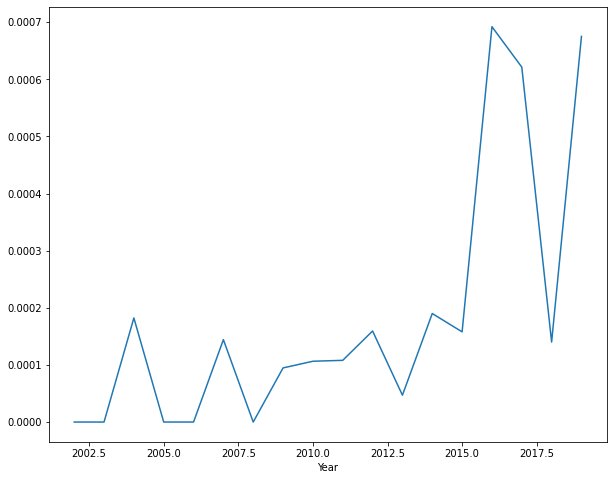
\includegraphics{notebooks/W04. Natural Language Processing_files/figure-pdf/cell-15-output-2.png}

}

\end{figure}

Regex can be pretty confusing, but it's also a very powerful tool.
Before moving on, let's familiarize ourselves a bit more with regex.

Back to climate change. Now we know the

\begin{Shaded}
\begin{Highlighting}[]
\NormalTok{re.findall(}\VerbatimStringTok{r"([\^{}.]*climate change[\^{}.]*)"}\NormalTok{,}\StringTok{" "}\NormalTok{.join(df[}\StringTok{\textquotesingle{}Text\textquotesingle{}}\NormalTok{]) )}
\end{Highlighting}
\end{Shaded}

\begin{verbatim}
[' However, as the world looks to lower their carbon emissions and respond to the risk of climate change, there is a desire to better understand how robust our plans are to evolving policies and changing market trends',
 ' Meeting the growing need for energy and addressing the risk of climate change are not mutually exclusive',
 " Over the past year, I've met with policymakers from both sides of the aisle: NGOs, academia, and participated in a climate change dialogue at the Vatican",
 '\n\nOur approach to climate change has 4 components',
 " We don't believe that society has to choose between economic prosperity and reducing the risk of climate change",
 '\n\nRecent steps the company has made in the last month to start to make arrangements for dialogue with the Climate Action 100+ group at independent director level are welcome, but the fact that it has taken so long to get to this point reflects how painfully slow progress has been to date with Exxon on climate change',
 ' I would tell you that we understand the concerns and share your desire to meaningfully address climate change, and I think ExxonMobil plays a pretty important role in that both today and in the future',
 " The Board's been engaged, and I would tell you, too, that we've had many, many discussions not only with your organization, but with many groups outside who have this concern, and I think are making very good progress in addressing some of the fundamental challenges associated with the risk of climate change",
 "\n\nMembers of the Board, this week's Economist describes ExxonMobil as a notable laggard on climate change",
 '\n\nThe next shareholder proposal calls for a specific Board climate change committee, and I understand that Natasha Lamb will present this proposal',
 ' Investor capital is at substantial risk in the face of climate change policy, competition from renewables, peak oil demand and unburnable fossil fuel reserves',
 ' This proposal seeks contractual clarity to ensure that the existential threats of climate change are being addressed in depth by the Board',
 ' Business strategy based on this assumption is unlikely to redirect company finances and innovative capacities to meet the formidable challenges posed by climate change and temperature containment goals',
 ' Establishing a Board committee with delineated duties can ensure that climate change is given adequate rather than tangential focus',
 ' A climate change committee can better inform and strengthen the entire Board, making it more climate-competent',
 ' A committee is a straightforward way for a Board to create clear lines of responsibility, a contractual level of clarity about who is responsible for overseeing and setting policy on climate change, and a delineation of liability for failure of care',
 ' We have a comprehensive framework to assess our business risk including the change and the risk associated with climate change',
 ' The proposal requests a report assessing the public health risks of expanding petrochemical operations in areas increasingly prone to climate change-induced storms, flooding and sea level rise',
 " It will further provide more transparent analysis to shareholders who must assess the strength of management's actions to mitigate risks from petrochemical investments in areas increasingly prone to climate change-induced storm, flooding and sea level rise",
 " We believe that more robust disclosure is needed to demonstrate leadership on corporate governance, and to mitigate reputational risks at a time of growing shareholder concern about misalignment between company's stated values and positions and their political activity, particularly on climate change issues",
 '\n\nThere are also concerns about the trade groups lobbying against responsible climate change policies',
 ' Recently, investors in Europe urged over 50 companies to ensure all lobbying related to climate change was consistent with the goals of the Paris accord',
 '\n\nOn the resolution concerning a climate change board committee, approximately 7',
 ' Texans are no strangers to the impacts of climate change',
 ' Meanwhile, communities on the Gulf Coast are still rebuilding their homes, and we know that more storms are on the way as climate change caused by your product makes extreme weather events more likely',
 ' I think if we step back and look at the risk associated with climate change, it comes back to emissions and the level of emissions globally emitted from energy sources',
 ' It says, "Wouldn\'t a board committee focused on climate change help assure that this broad societal risk impact on the company is regularly considered and assure shareholders that this issue is properly considered -- or is considered appropriately?" And then the concern is that failure to reassure the investing community, that this might have a negative impact on TSR',
 '\n\nSo maybe first of all, let me reiterate that the company recognizes that there are risks from climate change',
 ' Again, the company takes serious the risk from climate change and we are addressing that in many ways',
 "\n\nIt says regarding climate change, absent a committee focused on climate change, would the company be able to disclose information concerning each board member's knowledge on the subject?\n\nAgain, I think we mentioned, one of the enhancements we made in the proxy this year was to better identify the skills and the competencies that are important to the Board of Directors, and then to align or link those skills and competencies to the biographies of each director to ensure we appropriately address what skills are important to us and how the directors represent those skills and competencies",
 "\n\nAnd importantly, additional information about the risks associated with climate change, OIMS, process safety and environmental performance can be found already in ExxonMobil's energy and carbon summary, sustainability report and other publications, blogs and news releases",
 ' It says, "Wouldn\'t a board committee focused on climate change help assure that this broad societal risk impact on the company is regularly considered and assure shareholders that this issue is properly considered -- or is considered appropriately?" And then the concern is that failure to reassure the investing community, that this might have a negative impact on TSR',
 '\n\nSo maybe first of all, let me reiterate that the company recognizes that there are risks from climate change',
 ' Again, the company takes serious the risk from climate change and we are addressing that in many ways',
 "\n\nIt says regarding climate change, absent a committee focused on climate change, would the company be able to disclose information concerning each board member's knowledge on the subject?\n\nAgain, I think we mentioned, one of the enhancements we made in the proxy this year was to better identify the skills and the competencies that are important to the Board of Directors, and then to align or link those skills and competencies to the biographies of each director to ensure we appropriately address what skills are important to us and how the directors represent those skills and competencies",
 " We're also committed to being part of the solution in addressing the risk of climate change and other pressing societal challenges",
 '\n\nToday, many in society are looking for solutions that address the risk of climate change',
 " This disclosure addresses feedback from our shareholders, including the 2017 shareholder proposal, which received majority support at last year's shareholder meeting, that being the report on impacts of climate change policies",
 ' Pete Trelenberg is an expert in the climate change field; and Dr',
 " And they'll describe how we look at, how we evaluate and how we address the demand for energy and the risk of climate change",
 " That demand for energy and risk for climate change is what I have referred to in a number of the things that I've written, conversations [today]",
 " So I wondered whether you could talk a little bit more, sort of characterize where you are with that? And I say that because it was very clear that one of your peers sort of put out a view of energy not dissimilar to yours and was almost accused of being a climate change denier because the scenario they were showing, which is a practical one, didn't accord with what people wanted to see",
 "\n\nIn the afternoon, we'll then talk about climate change and how we're positioning ourselves for lower carbon energy future and the work that we're doing to address the risk of climate change",
 '\n\nLet me now turn to our mission, supplying energy for modern life, improving living standards around the world while minimizing the impact on the environment, including the risk of climate change',
 '\n\nFinally, we engage in public policy discussions on the best way to manage the risk of climate change',
 '\n\nWhile policy will play an enabling role, technology will be the key to addressing the risk of climate change and the growing need for energy',
 " It's also key to supplying the world's energy needs while mitigating the risk of climate change",
 ' We have a fundamental research program aimed at providing affordable and reliable energy for society, which will continue to underpin the research required to meet the dual challenge of delivering affordable and reliable energy while addressing the risks of climate change',
 ' For decades, we have provided technical depth and insights to complex energy issues including climate change and the safe use of fuels and chemicals',
 ' We face the challenge in meeting the needs of the growing population while mitigating the risk of climate change',
 '\n\nContinuing to grow high-cost fossil fuel reserve in the face of global climate change, disruptive technology development and the Paris climate agreement is no longer prudent',
 ' The Board agrees with the proponent that the risk of climate change is important to our business, but we do not agree with this approach',
 '\n\nThe next shareholder proposal calls for report on the impacts of climate change policies',
 ' At this meeting last year, I proposed a resolution asking ExxonMobil to undertake and disclose climate change scenario analysis',
 '\n\nMembers of the board, in your other roles, you have made clear that you recognize the significance of the agreed international goals on climate change',
 " Frazier, Merck's climate change position statement says Merck supports science-based international and national actions to address the challenges presented by climate change",
 '"\n\nMembers of the board, do you leave your understanding of climate change at the door when you attend ExxonMobil board meeting?\n\nExxonMobil said in its 2014 climate risk report to shareholders, "The 2 degrees is not a scenario worth considering',
 '\n\nWe believe the risks of climate change are serious and warrant action, thoughtful action',
 ' The board believes methane merits particular attention due to potential impacts on climate change',
 '\n\nOn the resolution concerning a report on impact of climate change policies, approximately 62',
 " Meeting society's need for energy while addressing risk of climate change",
 ' Acknowledges that risks of climate change are serious and warrant thoughtful action',
 ' Supporting long-range R&D to address climate change:\n\n1',
 ' Engaging on climate change:\n\n1',
 '\n\nI ask that you consider this information with regards to shareholder proposal Item #12, which is a report on impacts on climate change policies',
 " First, I'll note the dual challenge, that is, meeting society's need for energy while addressing the risk of climate change",
 "\n\nNext we state Exxon Mobil's position on climate change, which you can find on our website",
 ' We acknowledge that the risks of climate change are serious and they warrant our full action',
 "\n\nNext, I'll highlight our support for long life -- long-range research and development to address climate change",
 ' We support continued dialogue across all these venues to promote sound climate policy that provides for affordable energy solutions while also addressing the risk of climate change',
 ' Technology is also helping us to address the risk posed by climate change',
 ' We are in early days, but making carbon capture economic could lead to large-scale applications around the world, reducing emissions and mitigating the risk of climate change',
 ' Nowhere is this comprehensive cooperative approach more important than addressing the risk of climate change',
 '\n\nFor many years now, Exxon Mobil has held the view that the risks of climate change are serious, and they do warrant thoughtful action',
 ' We have long worked collaboratively with academic and institutional efforts to support research, improve climate models and advance the scientific understanding of climate change',
 " Our scientists have been participating with the UN's intergovernmental panel on climate change from its founding and have produced hundreds of publicly available papers including more than 50-peer-reviewed publications",
 '\n\nOn the policy front, we believe that addressing the risk of climate change is a global issue, which will require the involvement of governments, companies and all energy consumers',
 " We've taken thoughtful consistent action to protect the environment and to help understand and reduce the risk of climate change",
 " Because accountability and transparency are the key tenets of good governance, CalPERS has also been actively soliciting with The New York City Comptroller's office for Proposal Number seven concerning proxy access and Proposal Number 12 to improve the company's risk reporting concerning climate change risk",
 " We're asking for a person with climate change expertise to be on the Board for two main reasons",
 " Maybe if we would have had a climate change expert on the Board, she or he would not have allowed Exxon to act in the way they did when we first filed our shareholder resolution in 1997 on climate change or maybe they wouldn't have denied it for the first 10 years after we did file it",
 "\n\nEven as I speak today, the company is still supporting efforts, it seems, by some to undermine state's efforts to ensure the health of their people by having some kind of mitigation around climate change",
 "\n\nToday, at the meeting, we heard from CalPERS and CalPERS just issued a statement that from now on, they're going to be asking all companies to have somebody with climate change on their board",
 " If that's going to be for all companies, how much more for a company where almost 100% of our product and our efforts and production is related to climate change",
 " I think it's the first time, and you know I've been here quite a bit, where you begin with the problem of climate change and acknowledged it",
 ' Exxon presents a false choice between providing reliable and affordable energy and addressing climate change',
 '\n\nWe question whether lives will actually be improved in low-income communities if they are regularly suffering from the impacts of drought, extreme weather, geopolitical upheaval due to climate change and other factors',
 "\n\nThe proposed bylaw is intended to give substantial long-term shareowners a meaningful voice in electing the directors responsible for overseeing the company's long-term strategy and risks, including risks related to climate change",
 '\n\nIllustrating the deep international concern about lobbying and climate change, AP7, a Swedish pension fund, which owns over 3',
 ' Transparency and accountability in corporate spending to influence public policy are the best -- are in the best interest of ExxonMobil shareholders, and a high profile investigation into whether our company mislead investors on climate change only underscores the importance of full disclosure',
 ' ALEC has attracted negative attention for its role in promoting bills on anti-immigration policies, and also blocking EPA regulation on climate change',
 ' Continuing to grow high cost fossil fuel reserves in the face of global climate change disruptive agreement is no longer prudent',
 ' Every day, new reports and incidents demonstrate the importance of the 2-degree target for the sake of our planet for future generations and vulnerable communities, communities hit hardest by climate change',
 " Decades have been lost in the fight against climate change due in part to our company's deliberate campaign of disinformation",
 '\n\nThe next shareholder proposal calls for a report on impacts of climate change policies and is shown on Pages 69 and 70 of the proxy statement',
 '\n\nChairman, as you have acknowledged this morning, climate change is real',
 '\n\nChairman, the board is losing the confidence of its investors on climate change',
 '\n\nRecognizing the urgency facing businesses to respond to climate change, this proposal seeks to provide a means by which our company can move beyond the current business model, begin to respond to new opportunities and consider becoming an energy company for the future',
 '\n\nExxon publicly supports a carbon tax and acknowledges the realities of climate change, but its lobbying practices appear to conflict with his positions',
 " We believe that ExxonMobil shareholders deserve to understand the process by which the company contributes to organizations whose positions contradict Exxon's stated principles, blocking progress on climate change",
 " I've been a climate change scientist for nearly 50 years, and I'm here on behalf of Mercy Investment Services, speaking with respect to the items raised in Proposals 11 and 12",
 "\n\nOn the first point, in DOE's major, widely peer-reviewed 1985 climate change assessment that preceded IPCC, Exxon's leading climate change scientist for the past several decades, Dr",
 ' Brian Flannery, coauthored the chapter on projecting climate change',
 " But the reason I'm here kind of is this interest -- they used to call it global warming, but now it's called climate change",
 " Needless to say, my feeling is that the effects of climate change are real and are happening now, not something that's abstract and in the future, not something that's just been affecting indigenous populations, even though that's really heartbreaking as well",
 " I think from today's meeting, I know what your position is and whether Exxon should be held legally liable for damages from climate change",
 ' How is Exxon calculating the financial risks it would face if fossil fuel companies have to pay for damage from climate change, like the tobacco companies who, for many decades, said cigarettes were not an unhealthy thing to take part in',
 " So as state Attorneys General investigate whether ExxonMobil misled investors and the public about the realities and risks of climate change, people are increasingly making comparisons to the tobacco industry's misconduct and measures taken to address it",
 ' ExxonMobil now claims that quote, "We do not fund or support those who deny the reality of climate change',
 ' ExxonMobil is represented on the board of the American Petroleum Institute, API, which continues to claim that the science of climate change is unsettled, while attempting to block efforts to limit carbon pollution',
 ' And the fact that people have different opinions on climate change, they have every right to their opinion',
 " If we're not going to admit to climate change and admit that fossil fuels are causing -- are a part of climate change, so at least let's look at the health effects from the things that are coming out of the plants",
 '\n\nI do appreciate your admitting that there is climate change',
 "\n\nIn 1977, he briefed the company's top executives on the scientific realities of climate change",
 "\n\nMy question was going to be, will you withdraw funding from ALEC because they're known to spread misinformation about climate change, but it sounds like your answer on that is a resounding no",
 " So since you won't be doing that, will Exxon be taking action to, at all, refute or counteract the negative impacts they're making by funding an organization that says that climate change is a scam?\n\nREX TILLERSON: We will continue to engage in the policy discussions, as we currently do, with a number of broad-based groups on all sides of these issues and we'll continue to be active in the discussions legislatively in Washington and elsewhere, including through the IPCC on what we think are thoughtful, sensible policy actions that accommodate both our need for economic growth as well as addressing these risks, which are going to be very, very daunting",
 '\n\nOn the resolution concerning a report on impacts of climate change policies, approximately 38',
 ' All directors must possess capabilities to address full range of business risks, including those associated with risk of climate change',
 ' takes risk of climate change seriously',
 ' Long-term objective of climate change policy should be to reduce risk of harm at minimal societal cost, while providing reliable and affordable energy to improve global living standards',
 ' Report on impacts of climate change policies',
 ' Further, all Directors must possess the capabilities to address the full range of business risks, including those associated with the risk of climate change',
 '\n\nFirst among several climate-related proposals is one that seeks to increase capital distributions, meaning dividends and share purchases in light of climate change-related risks',
 ' To address questions raised on the topics of global energy demand and supply, climate change policy and carbon asset risk, the Company previously published a comprehensive report entitled, Energy and Carbon -- Managing the Risks',
 ' First, you should know that the Company takes the risk of climate change seriously and this risk requires thoughtful action',
 ' The long-term objective of climate change policy should be to reduce the risk of harm at minimal societal cost while also providing reliable and affordable energy to improve global living standards',
 '\n\nThe next climate policy is on a report on impacts of climate change policies',
 '\n\nAt ExxonMobil, we do take the risk of climate change seriously',
 ' We have studied climate change for almost 40 years, and we consistently collaborate and share our research with leading scientific institutions, top universities, the United Nations and other public stakeholders',
 ' We also engage in constructive dialogue on climate change policy options with NGOs, industry and policymakers',
 ' ExxonMobil received this proposal due to its exposure to risk related to climate change',
 '\n\nAs [Leward Brown], the former CEO of DP, warned in a speech last year, extractive industries need to take climate change more seriously or face an existential threat to their business',
 ' And I suspect -- put in context of my remarks, what we just heard -- not one word about climate change',
 ' Tillerson, you at least addressed the topic of climate change and alternatives',
 ' And silence speaks volumes on this, which means this Company is continuing business as usual when its competitors are at least giving lip service to the reality of climate change and the need',
 ' And so we wrote a shareholder resolution asking for somebody on the Board to have expertise on climate change',
 " But we've been -- the members of the Interfaith Centre on Corporate Responsibility started working on climate change in the late '80s",
 '\n\nJust in the last few weeks, the board of three of Exxon Mobil peers; BP, Shell, and Statoil, the board Members endorsed the shareholder resolution on climate change and carbon acid risk, underscoring just how material this issues is to the long-term future of the industry',
 "\n\nWe've spoken for many years about the urgency of climate change",
 ' And at the meeting at the Vatican last month, faith leaders noticed that human-induced climate change is a scientific reality and that decisive mitigation is a moral and religious imperative in humanity',
 "\n\nAnd I think one of the points I'd like to make about being in my first meeting is more and more treasurers and institutional investors are concerned about climate change and getting involved in this",
 '\n\nThe threats resulting from climate change are acute',
 ' We look forward to working with these various constituencies to realize our sustainability goals related to climate change while providing for the retirement security for the 48,000 [active investors] and retired members of the Vermont pension system',
 '\n\nIn the state of Vermont, the impacts of climate change are real, specifically our maple syrup industry, skiing industry, and the quality of our rivers, streams, and lakes are at risk with rising temperatures and increasingly volatile weather patterns',
 "\n\nTwo years ago in a speech that you were making in Cleveland, you brought up the issue of what happens if we can't stop climate change, if we can't address some of the issues that we've been talking about",
 " What's plan B?\n\nOur plan B has always been grounded in our beliefs around the continued evolution of technology and engineered solutions to address and react to whatever the climate system and its outcomes present to us, whether that be in the form of rises in sea level which we think you can address through different engineering accommodations along coastal areas, to changing agricultural production due to changes in weather patterns that may or may not be induced by climate change",
 ' We are very good in informative meeting in New York with executives around the issue of climate change and other issues',
 " And you all know we've been here before, that are ongoing issue is that the company isn't doing enough to address the crisis around climate change, now that was December",
 " In March the inter-government panel on climate change which this company has a part in it, said in effect first paragraph, climate change is already having sweeping effects on every continent and throughout the world's oceans, scientists just reported Monday",
 ' The effects of human induced climate change are being felt in every corner of the United States, scientists reported Tuesday',
 ' But our company continues to rely on a bet that the nations of the world will do nothing about climate change for the next 30 years',
 ' Channon], there was a [reward] and the topic was climate change',
 " My name is [Frank Rocher] a senior principal to Climate Associate (inaudible) Dallas, I'm here on behalf of the [Crystal Reynold's Foundation], the foundation with (inaudible) important climate change assumptions, here's for strategic planning following constructive discussions of Corporate Secretary, David Rosenthal and its calling December 17, 2013",
 ' Tillerson, you will require that if you talk to the council in formulations to during 2012, you said we have to be efficient and we have to manage climate change',
 " I view climate change as a risk management problem, what am I going to do about it the terms (inaudible) mitigation steps really different, that's plan B",
 " As you know, this include part of the international panel and the climate change, the US climate change assessment and we're seeing the military advisory board report on national security and the accelerated risk of climate change",
 "\n\nAnd by Mobil we'll also see for the nexus of energy in climate change as important",
 " Tillerson, what are the steps that you and the CEO of Exxon are doing to mitigate the risk of climate change? If these steps are not sufficient, what is your Plan B which we observed that the Cleveland requires steps now, how is Exxon Mobil using its resources to address the world's biggest energy challenge, how to meet global energy demand while addressing the potential disasters impact to climate on a global economy and or generally the whole global community?\n\nThe world's climate and energy requirements is a good beginning dialogue but didn't answer all these questions, I look forward to continuing dialogue which we have agreed upon with your colleagues on issues energy climate issues",
 "\n\nSo we all -- we do support and engage in and we'll continue to engage in active of dialogue and we're going to continue our active engagement with the UN's inter-governmental panel on climate change",
 "\n\nWe [now] look at that, and then look at other data, I see that according to the [few centers], the majority of Republicans don't believe that there is climate change, 90 percent of this company's political contributions are going to Republicans",
 " So on the one hand in this place, we hear you saying there is climate change, the burning of fossil fuels are human factor contributing to it, and yet you're going to support those very entities that are undermining the reality",
 '\n\nNow, what if this campaign said, Exxon Mobil says there is climate change, there is global warming, the burning of human fossil fuels are contributing to it and we got to do something because the world is at the door, everybody in the United States would know that we got to do something',
 ' It is interesting to note that the term global warming is now called climate change',
 ' Our think-tank once received contributions from the company, these contributions ended after the company told us it would not continue to contribute unless we adopted more alarm disposition on climate change',
 '\n\nAs a largest publically traded Energy Company with a mission of becoming the premier global energy company, I see it is our challenge and our duty to address greenhouse gas emissions and climate change, which faces our societies',
 '\n\nJust as we have taken on the challenge to discover new energy sources to drive modern societies, I think we also should be taking on the challenge of greenhouse gas and climate change and therefore I would highly recommend our shareholders to vote for resolution number 11 so that our company can also be one of those leaders',
 '\n\nREX TILLERSON: I think our views on climate change and the risk of climate change have been fairly well described both in public forums where I and others have spoken as well, as in publications in which we have expressed we view climate change as a serious issue, it does present serious risk',
 ' Over next 15 years, coal is expected to lose significant share as a result of climate change policies and a shift that favors a cleaner and diverse mix including more gas, nuclear and renewables',
 '\n\nWe have a report from the World Bank suggesting that if we continue with business as usual, and this is very much a business-as-usual kind of report, that by 2040 we will cross the two-degree threshold at which we have runaway climate change',
 ' Although there were references to emissions, there was no reference to the threat of runaway climate change',
 ' I wanted to ask another climate change question',
 ' Over the next 15 years, coal is expected to lose significant share as a result of climate change policies, and a shift that favors a cleaner and diverse mix, including more gas, nuclear, and renewables',
 '\n\nWe have a report from the World Bank suggesting that if we continue with business as usual, and this is very much a business-as-usual kind of report, that by 2040 we will cross the two-degree threshold at which we have runaway climate change',
 ' Although there were references to emissions, there was no reference to the threat of runaway climate change',
 ' I wanted to ask another climate change question',
 '\n\nFinally, t he industry is faced with risk of climate change and the resulting effect of government policies and impact on global markets',
 " I'm a filmmaker and an author and as part of a group that has traveled around the world looking at different communities and how they've been affected by the impacts of human cause climate change",
 '\n\nNow ExxonMobil , I believe, it was around 2008 made a commitment to stop funding denialist organizations and scientists whose purpose was to cast doubt on the reality of climate change and yet, in very recent news coming out of the United Kingdom, investigators showed that ExxonMobil was still funding some of these denialist organizations',
 ' Tillerson, in this now 2011 when there is consensus among the international scientific community that human cause climate change is a real threat that needs to be remedied, an action needs to be taken, will you make a personal promise on behalf of ExxonMobil to do what you can to stop funding denialist organizations and admit once and for all that human cause climate change is real and ExxonMobil is going to lead the way to do something about it',
 " That we view the risk from climate change as serious and it's a risk that does need to be managed in a very broad and global way",
 "\n\nWe do contribute to the broad based understand of the science underlying climate change and we have funded efforts on all sides of that issue at both the academic level and at private institutions because we think it's important on a policy that has such far reaching and dramatic impacts on society and our economic performance not just in this country but for the world, that we have the most fulsome discussion of what we understand bout this very complicated issue",
 '\n\nMICHAEL CROSBY: I just want to thank you very, very sincerely for what I heard in the remarks that you made about climate change',
 " We said climate change exists, we've said human factors are contributing",
 "\n\nJust a quick comment on your reaction to my remarks on climate change, they're not new",
 ' Tillerson, for the Company to actually step up and take leaderships instead of kind of hiding behind these positions in some way, yes you articulate it here, but you only talk really about climate change here in any kind of more forceful or clear way or when it comes to policy, how many times have you met with senators and congressmen on the Hill about a carbon tax',
 " I think we are a leader in these areas -- both in the climate change discussion and articulating for others our views and our position in trying to be a positive participant in very serious policy discussions, I could not count for you the number of discussions I've had with people on the Hill about carbon tax",
 " How the climate change issue is evolving from one year to the next it is looked at every year so that we get an update on is there anything new that's emerged in the science",
 '\n\nIn the context of these economic conditions, government policies that will influence climate change continue to be developed',
 '\n\nFinally, the industry is faced with risk of climate change and the resulting effect of government policies and impact on global markets',
 ' At ExxonMobil , we are taking a proactive approach to managing long-term risk of climate change',
 " On this very same issue of Exxon making really substantive, concrete progress on dealing with climate change and setting a comprehensive business strategy and plan for dealing with increased emissions from the Company and how you're going to get those down",
 ' It is undeniable that the rapid rate of climate change and carbon emission levels are a serious threat to humanity',
 ' And it asks for a report to share owners on the financial risks resulting from climate change and its impact on share owner value over time, as well as actions that the Board deems necessary to provide long-term protection of business interests in share owner value',
 '\n\nAnd so he felt that, with the Securities and Exchange Commission rules that were issued on February 8, 2010, interprets his guidance regarding disclosure related to climate change, that that will help',
 '\n\nAnd he felt that greater transparency on financial risk related to climate change is a very important issue both to ExxonMobil  and to all of the share owners',
 " Switching gears, I'd like to suggest that climate change is entirely natural",
 " According to Newsweek Magazine's March 1st edition, a Rasmussen poll last summer stated that 47% of all Americans believe that climate change was caused by man and only 33% believed it was caused by nature",
 '\n\nA new poll last winter showed that these numbers have flipped and now 47% of all Americans believe that climate change is completely natural',
 ' As time goes on, more and more American will realize that climate change is entirely natural and that these alarmists are promoting a scam and they continue to blow smoke up your pants every year',
 ' So, why believe they can project anything years ahead?\n\nThere is zero science to show that C02 in our biosphere is the cause of climate change up or down',
 ' And to the extent that climate change legislation creates advantages or disadvantages for fuel choices, natural gas clearly is a competitive fuel as a price for carbon might be put in place',
 ' And to the extent that climate change legislation creates advantages or disadvantages for fuel choices, natural gas clearly is a competitive fuel as a price for carbon might be put in place',
 " Clearly in the last ten years of our conversations around climate change, we now see it's another whole world, I would say, since even we were here last year",
 " To have constructive dialogue with Professor Boskin on climate change, and the implication for sustaining our company's stellar performance out into the future",
 "   \n\nNow climate change may be about our planet's future, but it's also about the financial implication to company's such as  ExxonMobil",
 ' Tillerson, you made no mention of issues of climate change or impact that that might have on the profitability over a company that is a multi-decade investor in the area',
 " Why has our company seemingly put so much effort into making itself into public enemy number one on climate change? How have we gotten to this point, where an otherwise great company who has acquired such a dismal reputation, and has become more known more for its funding of climate skeptics than for its technological leadership, which is quite profound?   \n\nIt just seemed irrational to me, you're an energy company, your job is to deliver returns to shareholders which you're quite good at, your job is not to be public philosophers on science, though I did enjoy your lecture last year in this meeting on the philosophical impossibility of scientific consensus",
 "   \n\nI guess perhaps you could claim that you've benefited shareholders by delaying the day of reckoning for  ExxonMobil on climate change, but I don't see that",
 '   \n\nYou can turn climate change into an opportunity if you want to, but instead you continue to fund groups like the Heartland Institute that question the science of climate change, and all you can really manage to say on the issue is that the risk from rising greenhouse gas emissions could prove to be significant',
 '   \n\nWhen you compare that to what some of your peers have said, the head of  ConocoPhillips a few weeks ago said that, "The science on climate change is quite compelling, human activity including the burning of fossil fuel is contributing to climate change',
 ' Now is the time for a national mandated framework to deal with climate change',
 '" And this is a clear statement, and this is a company that certainly understands the urgency of climate change',
 '   \n\nAnd you complain that your position on climate change is misunderstood, but with legalistic statements like the one I quoted, it just seems like you almost want to be misunderstood',
 " As you and I talked last year, I said that there is much we know and can agree on around the climate change issue, and there's much that we just don't believe we do know",
 ' The position that you described of others is not that different from our position on climate change',
 "   \n\nLast year Exxon gave $11 million to combat malaria, and educate girls and women in Africa, but what was in the news? It was the funding of think tanks and organizations that deny the science which is unequivocal, we've heard it, we've heard it before, enter governmental panel on climate change, 2,500 scientists",
 '   \n\nAnd as you know, many Bills are now presently being considered in Congress regarding climate change, some of which go by the name of Carbon Taxes, others by Cap and Trade Systems',
 ' All of which have really the same goal which is to reduce the amount of carbon that we are emitting into the atmosphere and to mitigate the worst effects of climate change',
 ' The strongest applause that you got today were for comments on your dedication to the difficult challenge of climate change',
 ' There is no more difficult challenge than climate change',
 "  \n\nThe company's strategy on climate change, as example filed by the recent report that was prepared with his committees explicit approval, demonstrates a startling and willful ignorance of an issue that we believe has the ability to dramatically reshape a landscape of the energy industry",
 "  \n\nOne of which the risk is great that we're actually increasing evidence of climate change by sharply curbing greenhouse gas emissions",
 ' And yet our company has produced an entire report on climate change that completely ignores the issue of whether rising greenhouse gas emissions will in anyway impact the market for energy',
 '  \n\nOur competitors are increasingly understanding that climate change poses a fundamental threat to where they do business? And the competitors are reported to drive under virtually any future scenario',
 '  \n\nWhile our companies prepare only for one, the rather unlikely scenario of the climate change is a myth and business as usual continues for the next several decades',
 " They are concerned about Exxon strategy for climate change and they're very much interested in the company taking a leading role in developing renewable energy for our country in the global market",
 "  \n\nInstitutional investors are also increasingly concerned about the company's position on climate change, including some of the largest public pension in the US",
 ' Your position on climate changes completely obscured your progress in other areas of corporate transparency and responsibility and therefore does no service to this company and its shareholders',
 " I'd like to know what provisions you have made on the financial statements for damage caused by climate change? Climate change is the potential liability and I wonder if you have reserved for it on the balance sheet?  \n\nRICHARD PATTERSON, EXXON MOBIL CORPORATION: The responsibility for provisions in the financial statement are those of management and I am not sure that I am the appropriate person to respond to that question",
 " Have -- what provisions have you made on the financial statement for the damages caused by climate change and the potential liability there and have you reserved for it?  \n\nRICHARD PATTERSON: It's neither likely nor could it be estimated",
 ' We were happy to see or to hear about a report that was going to be published by our company on climate change',
 ' The climate change and the policy to be listed, or have the potential for dramatically reshape the economic landscape of our energy industries',
 "  \n\nAs subjects on Mobil strategy with respect to climate change, is a key to company's long-term health, as a company",
 ' For this company is sticked out a position of willful ignorance on climate change',
 " The Company's policy on climate change is so tied up with you",
 ' Chairman our resolution, ask the company to report the data it uses to develop its position on the science of climate change',
 " Second, global warming has become a drag on a company's reputation the problem go beyond the global boycott they continue to hamper sales over the last years state pension funds and main stream equity analyst have joined the course of those asking for our company to be more accountable on the risks of climate change",
 '  \n\nYour existing statements on global climate change as well as your significant financial commitment to Stanford University and other institutions are evidence that you take this responsibility seriously',
 ' I want to strongly support, the request for greater disclosure on climate change',
 " I'm concerned of the shareholder and I have represented other shareholders that we are increasingly being left behind by our key competitors preparing to deal with issue of climate change",
 ' Our competitors are frequently demonstrating that they understand the climate change process is a fundamental threat to way - that they do business',
 ' No one has still questioned the science on climate change',
 "  \n\nAll even have publicly agreed with the consensus of word scientist, the climate change is a real threat it's caused by human activity",
 ' BP and Shell are investing in renewables to hedge the risk of climate change',
 ' Howell Fitz, has pledged the shareholders available to disclose sometime this year, the actual financial impact of climate change on the company going-forward',
 ' The Boards would bubble said the proposals state - quote " Our scientists have authored nearly 60 papers in scientific and technical publications on climate change with over 30 published and peer reviewed journals" -- unquote',
 " If you wanted to do more, you will give the names of the scientists who'd be nominated to serve in a numerous review board, listing their names and listing the review boards including those acting as legal authors with the intergovernmental panel and climate change",
 " All those, would verifiably prove Exxon Mobil's interest in climate change beyond any shadow of a doubt",
 ' Nowhere in this resolution does it say that Exxon Mobil has to agree with us on the science of climate change',
 ' And so, here we are to propose this resolution, which is intended to begin a dialogue with the company, with its management and with its Board of Directors about the science of climate change and whether this company has engaged in a real historical process to determine its own position',
 ' Right now, we have the information for our side the Intergovernmental Panel on climate changes has provided a great set of reports']
\end{verbatim}

The earnings call transcript is structured in such a way that it should
be possible to separate speakers based on regular expressions. Every
time a new person is speaking, they are introduced in the transcript in
a new paragraph; Consider the excerpt below:

\begin{verbatim}
OPERATOR: Our next question comes from Philip Weiss with Argus Research.

PHILIP WEISS, ANALYST, ARGUS RESEARCH COMPANY: Good morning. I did have one, most of my questions have been answered, but I do have one follow-up on the US. You said that the rig count that's being used for liquids-rich is rising but when I look at production, natural gas as a percentage of your total production has grown, and liquids has actually fallen a little bit. So, I wonder if you can just comment on when we might start to see that trend change?

DAVID ROSENTHAL: Sure. The fall off in the liquids is really just the overall decline in the conventional, as well as some divestments. You'll recall we had a divestment in the Eastern Gulf of Mexico and that had an impact on us year-over-year in particularly in the second half.
In terms of when we'll see significant production growth out of the unconventional, I mentioned some of the increases in percentages, although we haven't given all of the specific production volumes, but we'll do that as we progress.
\end{verbatim}

Now, we can't simply split by new line (\texttt{\textbackslash{}n});
David Rosenthal has two paragraphs. We also can't just split using
\texttt{:}, since this may appear in the text. Let's describe the
features of the names we're looking to split out:

\begin{enumerate}
\def\labelenumi{\arabic{enumi}.}
\tightlist
\item
  It's a single or group of words * regex: \texttt{(\textbackslash{}w)}
\item
  The words are all caps, and can contain any characters *
  regex:\texttt{(\textbackslash{}w{[}A-Z{]})}
\item
  There are multiple words, and they can be separated by anything *
  regex:
  \texttt{(\textbackslash{}w{[}A-Z{]}+.+\textbackslash{}w{[}A-Z{]})}
\item
  The sequence always ends in a colon * regex:
  \texttt{(\textbackslash{}w{[}A-Z{]}+.+\textbackslash{}w{[}A-Z{]}+:)}
\end{enumerate}

If we plug this into

\begin{Shaded}
\begin{Highlighting}[]
\NormalTok{re.findall(}\VerbatimStringTok{r\textquotesingle{}([A{-}Z]+.+[A{-}Z]+:)\textquotesingle{}}\NormalTok{, call[}\StringTok{\textquotesingle{}Text\textquotesingle{}}\NormalTok{])}
\end{Highlighting}
\end{Shaded}

\begin{verbatim}
['JEFF WOODBURY, VP OF INVESTOR RELATIONS, CORPORATE SECRETARY, EXXONMOBIL CORPORATION:',
 'REX TILLERSON:',
 'REX TILLERSON:',
 'REX TILLERSON:',
 'BETH RICHTMAN, INVESTMENT MANAGER, CALPERS:',
 'REX TILLERSON:',
 'MICHAEL CROSBY, CAPUCHIN FRANCISCAN FRIAR:',
 'REX TILLERSON:',
 'TRACEY REMBERT, SHAREHOLDER, CHRISTIAN BROTHERS INVESTMENT SERVICES:',
 'REX TILLERSON:',
 'MICHAEL GARLAND, ASSISTANT COMPTROLLER FOR CORPORATE GOVERNANCE AND RESPONSIBLE INVESTMENT, OFFICE OF NEW YORK CITY COMPTROLLER:',
 'REX TILLERSON:',
 'TOM SIFFERMAN, REPRESENTATIVE, MOBIL OIL:',
 'REX TILLERSON:',
 'HUGHES JENKINS, EMPLOYEE, UNITED STEELWORKERS:',
 'REX TILLERSON:',
 'NATASHA LAMB, DIRECTOR OF EQUITY RESEARCH, ARJUNA CAPITAL AND BALDWIN BROTHERS:',
 'REX TILLERSON:',
 'PATRICIA DALY, SISTERS OF ST. DOMINIC OF CALDWELL NEW JERSEY:',
 'REX TILLERSON:',
 'PATRICIA DALY:',
 'REX TILLERSON:',
 'EDWARD MASON, SHAREHOLDER, CHURCH COMMISSIONERS FOR ENGLAND:',
 'REX TILLERSON:',
 'DANIELLE FUGERE:',
 'REX TILLERSON:',
 'DANIELLE FUGERE:',
 'REX TILLERSON:',
 'REX TILLERSON:',
 'REX TILLERSON:',
 'DAVID RIESMAN, SHAREHOLDER:',
 'REX TILLERSON:',
 'DAVID RIESMAN:',
 'REX TILLERSON:',
 'MICHAEL MACCRACKEN, CHIEF SCIENTIST, CLIMATE CHANGE SCIENTIST, MERCY INVESTMENT SERVICES:',
 'REX TILLERSON:',
 'MICHAEL MACCRACKEN:',
 'REX TILLERSON:',
 'DAVID MARTINEAU, GEOLOGIST:',
 'REX TILLERSON:',
 'RENEE BOUCHARD:',
 'REX TILLERSON:',
 'KATHY MULVEY, ACCOUNTABILITY CAMPAIGN MANAGER, UNION OF CONCERNED SCIENTISTS:',
 'REX TILLERSON:',
 'KATHY MULVEY:',
 'REX TILLERSON:',
 'CHARLOTTE RAWLS, SHAREHOLDER:',
 'REX TILLERSON:',
 'CHARLOTTE RAWLS:',
 'REX TILLERSON:',
 "ROBERT FORE, REPRESENTATIVE, PRESBYTERIAN CHURCH U.S.A.'S FOUNDATION:",
 'REX TILLERSON:',
 'HUNTER MARTIN, SHAREHOLDER:',
 'REX TILLERSON:',
 'HUNTER MARTIN:',
 'REX TILLERSON:',
 'ANNA KOLINSKI:',
 'REX TILLERSON:',
 'REX TILLERSON:',
 'REX TILLERSON:',
 'UNIDENTIFIED AUDIENCE MEMBER:',
 'REX TILLERSON:',
 'JULIAN MARTINEZ, REPRESENTATIVE, SER-JOBS FOR PROGRESS:',
 'REX TILLERSON:',
 'REX TILLERSON:',
 'UNIDENTIFIED COMPANY REPRESENTATIVE:',
 'REX TILLERSON:']
\end{verbatim}

\begin{Shaded}
\begin{Highlighting}[]
\NormalTok{re.split(}\VerbatimStringTok{r\textquotesingle{}([A{-}Z]+.+[A{-}Z]+:)\textquotesingle{}}\NormalTok{, call[}\StringTok{\textquotesingle{}Text\textquotesingle{}}\NormalTok{])[}\DecValTok{9}\NormalTok{]}
\end{Highlighting}
\end{Shaded}

\begin{verbatim}
'BETH RICHTMAN, INVESTMENT MANAGER, CALPERS:'
\end{verbatim}

The kind of analysis we will be doing reqires \emph{tokenizing} a text,
and \emph{tagging} individual words. Tokenizing means splitting the text
into individul sentences or individual words, while tagging means
classifying each word according to a POS (Parts Of Speech)
classification. We can word tokenize our data using the
\texttt{word\_tokenize} function from the \texttt{nltk} library, which
returns an object which is a list of tokens; if we print the first 19
tokens, we get the first sentence:

\begin{Shaded}
\begin{Highlighting}[]
\NormalTok{  tokens}\OperatorTok{=}\NormalTok{nltk.word\_tokenize(call[}\StringTok{\textquotesingle{}Text\textquotesingle{}}\NormalTok{])  }
\NormalTok{  tokens[:}\DecValTok{19}\NormalTok{]}
\end{Highlighting}
\end{Shaded}

\begin{verbatim}
['I',
 "'m",
 'Rex',
 'Tillerson',
 ',',
 'I',
 "'m",
 'the',
 'Chairman',
 'and',
 'Chief',
 'Executive',
 'Officer',
 'of',
 'the',
 'Exxon',
 'Mobil',
 'Corporation',
 '.']
\end{verbatim}

Having tokenized our text, there are a number of useful functions can
use to explore it quantitatively. Let's start by counting the number of
times ``climate'' is mentioned:

\begin{Shaded}
\begin{Highlighting}[]
\NormalTok{tokens.count(}\StringTok{\textquotesingle{}climate\textquotesingle{}}\NormalTok{)}
\end{Highlighting}
\end{Shaded}

\begin{verbatim}
76
\end{verbatim}

\begin{Shaded}
\begin{Highlighting}[]
\NormalTok{nltk.Text(tokens).collocations()}
\end{Highlighting}
\end{Shaded}

\begin{verbatim}
REX TILLERSON; climate change; proxy statement; Exxon Mobil; Mr.
Tillerson; voting thereon; resolution concerning; per day; shares
voting; health care; Good morning; New York; Annual Meeting; barrels
per; natural gas; shareholder proposal; global warming; oil
equivalent; last year; York City
\end{verbatim}

\begin{Shaded}
\begin{Highlighting}[]
\CommentTok{\#nltk.Text(tokens).concordance(\textquotesingle{}climate change\textquotesingle{})}
\end{Highlighting}
\end{Shaded}

\begin{verbatim}
['EXXONMOBIL CORPORATION:',
 'REX TILLERSON:',
 'REX TILLERSON:',
 'REX TILLERSON:',
 'CALPERS:',
 'REX TILLERSON:',
 'CAPUCHIN FRANCISCAN FRIAR:',
 'REX TILLERSON:',
 'CHRISTIAN BROTHERS INVESTMENT SERVICES:',
 'REX TILLERSON:',
 'OFFICE OF NEW YORK CITY COMPTROLLER:',
 'REX TILLERSON:',
 'MOBIL OIL:',
 'REX TILLERSON:',
 'UNITED STEELWORKERS:',
 'REX TILLERSON:',
 'ARJUNA CAPITAL AND BALDWIN BROTHERS:',
 'REX TILLERSON:',
 'DOMINIC OF CALDWELL NEW JERSEY:',
 'REX TILLERSON:',
 'PATRICIA DALY:',
 'REX TILLERSON:',
 'CHURCH COMMISSIONERS FOR ENGLAND:',
 'REX TILLERSON:',
 'DANIELLE FUGERE:',
 'REX TILLERSON:',
 'DANIELLE FUGERE:',
 'REX TILLERSON:',
 'REX TILLERSON:',
 'REX TILLERSON:',
 'SHAREHOLDER:',
 'REX TILLERSON:',
 'DAVID RIESMAN:',
 'REX TILLERSON:',
 'MERCY INVESTMENT SERVICES:',
 'REX TILLERSON:',
 'MICHAEL MACCRACKEN:',
 'REX TILLERSON:',
 'GEOLOGIST:',
 'REX TILLERSON:',
 'RENEE BOUCHARD:',
 'REX TILLERSON:',
 'UNION OF CONCERNED SCIENTISTS:',
 'REX TILLERSON:',
 'KATHY MULVEY:',
 'REX TILLERSON:',
 'SHAREHOLDER:',
 'REX TILLERSON:',
 'CHARLOTTE RAWLS:',
 'REX TILLERSON:',
 'S FOUNDATION:',
 'REX TILLERSON:',
 'SHAREHOLDER:',
 'REX TILLERSON:',
 'HUNTER MARTIN:',
 'REX TILLERSON:',
 'ANNA KOLINSKI:',
 'REX TILLERSON:',
 'REX TILLERSON:',
 'REX TILLERSON:',
 'UNIDENTIFIED AUDIENCE MEMBER:',
 'REX TILLERSON:',
 'JOBS FOR PROGRESS:',
 'REX TILLERSON:',
 'REX TILLERSON:',
 'UNIDENTIFIED COMPANY REPRESENTATIVE:',
 'REX TILLERSON:']
\end{verbatim}

\begin{Shaded}
\begin{Highlighting}[]
\ImportTok{from}\NormalTok{ nltk }\ImportTok{import}\NormalTok{ bigrams}

\NormalTok{finder }\OperatorTok{=}\NormalTok{ BigramCollocationFinder.from\_words(tokens)}
\NormalTok{bigram\_measures }\OperatorTok{=}\NormalTok{ nltk.collocations.BigramAssocMeasures()}
\BuiltInTok{print}\NormalTok{(finder.nbest(bigram\_measures.pmi, }\DecValTok{2}\NormalTok{))}
\end{Highlighting}
\end{Shaded}

\begin{verbatim}
[('1,000', 'academics'), ('1,400', 'Gulf')]
\end{verbatim}

\begin{Shaded}
\begin{Highlighting}[]
\KeywordTok{def}\NormalTok{ tokenize(raw\_text):}
\NormalTok{  tokens}\OperatorTok{=}\NormalTok{nltk.word\_tokenize(raw\_text)}
\NormalTok{  text}\OperatorTok{=}\NormalTok{nltk.Text(tokens)}
  \ControlFlowTok{return}\NormalTok{ text}

\NormalTok{df[}\StringTok{\textquotesingle{}Text\textquotesingle{}}\NormalTok{]}\OperatorTok{=}\NormalTok{df[}\StringTok{\textquotesingle{}Text\textquotesingle{}}\NormalTok{].}\BuiltInTok{apply}\NormalTok{(}\KeywordTok{lambda}\NormalTok{ x: tokenize(x))}
\end{Highlighting}
\end{Shaded}

\begin{Shaded}
\begin{Highlighting}[]
\NormalTok{df[}\StringTok{\textquotesingle{}climate\textquotesingle{}}\NormalTok{]}\OperatorTok{=}\NormalTok{df[}\StringTok{\textquotesingle{}Text\textquotesingle{}}\NormalTok{].}\BuiltInTok{apply}\NormalTok{(}\KeywordTok{lambda}\NormalTok{ x: x.count(}\StringTok{\textquotesingle{}climate\textquotesingle{}}\NormalTok{))}
\NormalTok{df.plot(}\StringTok{\textquotesingle{}climate\textquotesingle{}}\NormalTok{)}
\end{Highlighting}
\end{Shaded}

\begin{verbatim}
<matplotlib.axes._subplots.AxesSubplot at 0x7fd4956abb90>
\end{verbatim}

\begin{figure}[H]

{\centering \includegraphics{notebooks/W04. Natural Language Processing_files/figure-pdf/cell-25-output-2.png}

}

\end{figure}

\begin{Shaded}
\begin{Highlighting}[]
\NormalTok{call}\OperatorTok{=}\NormalTok{df.iloc[}\DecValTok{38}\NormalTok{]}

\NormalTok{text}\OperatorTok{=}\NormalTok{call[}\StringTok{\textquotesingle{}Text\textquotesingle{}}\NormalTok{]}
\CommentTok{\#tokens=nltk.word\_tokenize(raw\_text)}
\CommentTok{\#text=nltk.Text(tokens)}

\NormalTok{word\_fd }\OperatorTok{=}\NormalTok{ nltk.FreqDist(filtered\_sentence)}

\NormalTok{text.concordance(}\StringTok{\textquotesingle{}climate\textquotesingle{}}\NormalTok{)}
\BuiltInTok{print}\NormalTok{(text.count(}\StringTok{\textquotesingle{}climate change\textquotesingle{}}\NormalTok{))}

\NormalTok{text.dispersion\_plot([}\StringTok{\textquotesingle{}climate\textquotesingle{}}\NormalTok{])}
\end{Highlighting}
\end{Shaded}

\begin{verbatim}
NameError: ignored
\end{verbatim}

\hypertarget{scatter-text}{%
\section{Scatter Text}\label{scatter-text}}

\begin{Shaded}
\begin{Highlighting}[]
\NormalTok{ceo\_df}\OperatorTok{=}\NormalTok{df[}\DecValTok{30}\NormalTok{:}\DecValTok{40}\NormalTok{]}
\NormalTok{ceo\_df[}\StringTok{\textquotesingle{}CEO\textquotesingle{}}\NormalTok{]}\OperatorTok{=}\NormalTok{np.where(ceo\_df[}\StringTok{\textquotesingle{}Date\textquotesingle{}}\NormalTok{]}\OperatorTok{\textgreater{}}\StringTok{\textquotesingle{}01{-}01{-}2017\textquotesingle{}}\NormalTok{,}\StringTok{\textquotesingle{}Woods\textquotesingle{}}\NormalTok{,}\StringTok{\textquotesingle{}Tillerson\textquotesingle{}}\NormalTok{)}

\ImportTok{import}\NormalTok{ scattertext }\ImportTok{as}\NormalTok{ st}

\NormalTok{corpus }\OperatorTok{=}\NormalTok{ st.CorpusFromPandas(ceo\_df,}
\NormalTok{                             category\_col}\OperatorTok{=}\StringTok{\textquotesingle{}CEO\textquotesingle{}}\NormalTok{,}
\NormalTok{                             text\_col}\OperatorTok{=}\StringTok{\textquotesingle{}Text\textquotesingle{}}\NormalTok{,}
\NormalTok{                             nlp}\OperatorTok{=}\NormalTok{nlp).build()}
\end{Highlighting}
\end{Shaded}

\begin{Shaded}
\begin{Highlighting}[]
\NormalTok{corpus}\OperatorTok{=}\NormalTok{corpus.remove\_terms(nlp.Defaults.stop\_words, ignore\_absences}\OperatorTok{=}\VariableTok{True}\NormalTok{)}
\end{Highlighting}
\end{Shaded}

\begin{Shaded}
\begin{Highlighting}[]
\NormalTok{html }\OperatorTok{=}\NormalTok{ st.produce\_scattertext\_explorer(}
\NormalTok{                   corpus,}
\NormalTok{                   category}\OperatorTok{=}\StringTok{\textquotesingle{}Woods\textquotesingle{}}\NormalTok{,}
\NormalTok{                   category\_name}\OperatorTok{=}\StringTok{\textquotesingle{}Woods\textquotesingle{}}\NormalTok{,}
\NormalTok{                   not\_category\_name}\OperatorTok{=}\StringTok{\textquotesingle{}Tillerson\textquotesingle{}}\NormalTok{,}
\NormalTok{                   width\_in\_pixels}\OperatorTok{=}\DecValTok{1000}\NormalTok{)}

\NormalTok{display(HTML(html))}
\end{Highlighting}
\end{Shaded}

\begin{Shaded}
\begin{Highlighting}[]
\NormalTok{df[}\StringTok{\textquotesingle{}Text\textquotesingle{}}\NormalTok{]}\OperatorTok{=}\NormalTok{df[}\StringTok{\textquotesingle{}Text\textquotesingle{}}\NormalTok{].}\BuiltInTok{str}\NormalTok{.split(}\StringTok{\textquotesingle{}}\CharTok{\textbackslash{}n\textbackslash{}n}\StringTok{\textquotesingle{}}\NormalTok{)}
\NormalTok{paragraphs}\OperatorTok{=}\NormalTok{df.explode(}\StringTok{\textquotesingle{}Text\textquotesingle{}}\NormalTok{)}
\NormalTok{paragraphs}
\end{Highlighting}
\end{Shaded}

\begin{Shaded}
\begin{Highlighting}[]
\NormalTok{paragraphs[}\StringTok{\textquotesingle{}speaker\textquotesingle{}}\NormalTok{]}\OperatorTok{=}\NormalTok{paragraphs[}\StringTok{\textquotesingle{}Text\textquotesingle{}}\NormalTok{].}\BuiltInTok{str}\NormalTok{.split(}\StringTok{\textquotesingle{}:\textquotesingle{}}\NormalTok{).}\BuiltInTok{str}\NormalTok{[}\DecValTok{0}\NormalTok{]}
\NormalTok{paragraphs}
\end{Highlighting}
\end{Shaded}

\begin{Shaded}
\begin{Highlighting}[]
\ImportTok{from}\NormalTok{ spacy.matcher }\ImportTok{import}\NormalTok{ PhraseMatcher}

\NormalTok{matcher }\OperatorTok{=}\NormalTok{ PhraseMatcher(nlp.vocab)}
\NormalTok{matcher.add(}\StringTok{"cc"}\NormalTok{, [nlp(}\StringTok{"carbon capture"}\NormalTok{)])}
\NormalTok{matches }\OperatorTok{=}\NormalTok{ matcher(doc)}

\NormalTok{ix}\OperatorTok{=}\NormalTok{matches[}\DecValTok{0}\NormalTok{]}

\NormalTok{doc[ix[}\DecValTok{1}\NormalTok{]}\OperatorTok{{-}}\DecValTok{10}\NormalTok{:ix[}\DecValTok{2}\NormalTok{]}\OperatorTok{+}\DecValTok{10}\NormalTok{]}
\end{Highlighting}
\end{Shaded}

\begin{Shaded}
\begin{Highlighting}[]
\ImportTok{from}\NormalTok{ spacy.matcher }\ImportTok{import}\NormalTok{ PhraseMatcher}

\NormalTok{phrase\_matcher }\OperatorTok{=}\NormalTok{ PhraseMatcher(nlp.vocab)}
\NormalTok{phrase\_list }\OperatorTok{=}\NormalTok{ [nlp(}\StringTok{\textquotesingle{}climate change\textquotesingle{}}\NormalTok{)]}
\NormalTok{phrase\_matcher.add(}\StringTok{"Text Extractor"}\NormalTok{, }\VariableTok{None}\NormalTok{, }\OperatorTok{*}\NormalTok{phrase\_list)}
\NormalTok{matched\_items }\OperatorTok{=}\NormalTok{ phrase\_matcher(doc)}

\NormalTok{matched\_text }\OperatorTok{=}\NormalTok{ []}

\ControlFlowTok{for}\NormalTok{ match\_id, start, end }\KeywordTok{in}\NormalTok{ matched\_items:}
\NormalTok{    text }\OperatorTok{=}\NormalTok{ nlp.vocab.strings[match\_id]}
\NormalTok{    span }\OperatorTok{=}\NormalTok{ doc[start: end]}
\NormalTok{    matched\_text.append(span.sent)}

\NormalTok{matched\_text}
\end{Highlighting}
\end{Shaded}

\begin{Shaded}
\begin{Highlighting}[]
\NormalTok{displacy.render(matched\_text[}\DecValTok{1}\NormalTok{], jupyter}\OperatorTok{=}\VariableTok{True}\NormalTok{)}
\end{Highlighting}
\end{Shaded}

\begin{Shaded}
\begin{Highlighting}[]
\ImportTok{import}\NormalTok{ textacy.extract}

\NormalTok{kwic}\OperatorTok{=}\NormalTok{textacy.extract.kwic.keyword\_in\_context(doc, }\StringTok{\textquotesingle{}global warming\textquotesingle{}}\NormalTok{)}

\ControlFlowTok{for}\NormalTok{ a }\KeywordTok{in}\NormalTok{ kwic:}
  \BuiltInTok{print}\NormalTok{(a)}
\end{Highlighting}
\end{Shaded}

\begin{Shaded}
\begin{Highlighting}[]
\ImportTok{from}\NormalTok{ spacy }\ImportTok{import}\NormalTok{ displacy}
\NormalTok{displacy.render(sentences[}\DecValTok{1}\NormalTok{], jupyter}\OperatorTok{=}\VariableTok{True}\NormalTok{)}
\end{Highlighting}
\end{Shaded}

\begin{Shaded}
\begin{Highlighting}[]
\ImportTok{from}\NormalTok{ collections }\ImportTok{import}\NormalTok{ Counter, defaultdict}

\KeywordTok{def}\NormalTok{ find\_character\_occurences(doc):}
    \CommentTok{"""}
\CommentTok{    Return a list of actors from \textasciigrave{}doc\textasciigrave{} with corresponding occurences.}
\CommentTok{    }
\CommentTok{    :param doc: Spacy NLP parsed document}
\CommentTok{    :return: list of tuples in form}
\CommentTok{        [(\textquotesingle{}elizabeth\textquotesingle{}, 622), (\textquotesingle{}darcy\textquotesingle{}, 312), (\textquotesingle{}jane\textquotesingle{}, 286), (\textquotesingle{}bennet\textquotesingle{}, 266)]}
\CommentTok{    """}
    
\NormalTok{    characters }\OperatorTok{=}\NormalTok{ Counter()}
    \ControlFlowTok{for}\NormalTok{ ent }\KeywordTok{in}\NormalTok{ doc.ents:}
        \ControlFlowTok{if}\NormalTok{ ent.label\_ }\OperatorTok{==} \StringTok{\textquotesingle{}PERSON\textquotesingle{}}\NormalTok{:}
\NormalTok{            characters[ent.lemma\_] }\OperatorTok{+=} \DecValTok{1}
            
    \ControlFlowTok{return}\NormalTok{ characters.most\_common()}

\BuiltInTok{print}\NormalTok{(find\_character\_occurences(doc)[:}\DecValTok{20}\NormalTok{])}
\end{Highlighting}
\end{Shaded}

\begin{Shaded}
\begin{Highlighting}[]
\NormalTok{text.dispersion\_plot([}\StringTok{\textquotesingle{}Grail\textquotesingle{}}\NormalTok{,}\StringTok{\textquotesingle{}rabbit\textquotesingle{}}\NormalTok{,}\StringTok{\textquotesingle{}Knights\textquotesingle{}}\NormalTok{,}\StringTok{\textquotesingle{}Ni\textquotesingle{}}\NormalTok{,}\StringTok{\textquotesingle{}castle\textquotesingle{}}\NormalTok{])}
\end{Highlighting}
\end{Shaded}

\begin{Shaded}
\begin{Highlighting}[]
\ControlFlowTok{for}\NormalTok{ token }\KeywordTok{in}\NormalTok{ doc:}
    \BuiltInTok{print}\NormalTok{(token.text, token.pos\_, token.ent\_)}
\end{Highlighting}
\end{Shaded}

\hypertarget{dirty-words-1}{%
\section{Dirty Words}\label{dirty-words-1}}

Text often comes `unclean' either containing tags such as HTML (or XML),
or has other issues, but fortunately we will be using `clean' sources,
at least initially. Be cautious when committing to a text analysis
project - you may spend a great deal of time tidying up your text.

The kind of analysis we will be doing reqires \emph{tokenizing} a text,
and \emph{tagging} individual words. Tokenizing means splitting the text
into individul sentences or individual words, while tagging means
classifying each word according to a POS (Parts Of Speech)
classification.

\hypertarget{the-castle-of-aaargh}{%
\section{The Castle of Aaargh}\label{the-castle-of-aaargh}}

We will first experiment with nltk and its built in corpus texts. We'll
work with some Monty Python, beloved of comedy bores for half a century

\hypertarget{setup}{%
\section{Setup}\label{setup}}

\begin{itemize}
\tightlist
\item
  install nltk through package manager, or the command line
\item
  import nltk
\item
  type nltk.download(`book'). This will automatically download the books
  into our workspace
\end{itemize}

\begin{Shaded}
\begin{Highlighting}[]
\CommentTok{\#nltk: natural language processing toolkit}
\ImportTok{import}\NormalTok{ nltk}
\end{Highlighting}
\end{Shaded}

\begin{Shaded}
\begin{Highlighting}[]
\CommentTok{\#Download the sample books}
\NormalTok{nltk.download(}\StringTok{\textquotesingle{}book\textquotesingle{}}\NormalTok{)}
\end{Highlighting}
\end{Shaded}

Now, we import the sample texts. You'll notice that text6 is ``Monty
Python and the Holy Grail'', as promised. Presumably this was compiled
pre-\emph{Spamalot}.

\begin{Shaded}
\begin{Highlighting}[]
\CommentTok{\#Import all features from nltk.book}
\ImportTok{from}\NormalTok{ nltk.book }\ImportTok{import} \OperatorTok{*}
\end{Highlighting}
\end{Shaded}

Let's look at the object text6; we can look at the first few words..

\begin{Shaded}
\begin{Highlighting}[]
\CommentTok{\#View the first ten words of text6}
\NormalTok{text6[}\DecValTok{1}\NormalTok{:}\DecValTok{10}\NormalTok{]}
\end{Highlighting}
\end{Shaded}

Which are presumably stage directions rather than dialogue. How many
words/symbols are in the text?

\begin{Shaded}
\begin{Highlighting}[]
\CommentTok{\#View the length of the list}
\BuiltInTok{len}\NormalTok{(text6)}
\end{Highlighting}
\end{Shaded}

Bear in mind that a lot of the functions we will carry out rely on this
being a text object - we'll start to think about how we use free text
and convert it to a \textbf{Text} object later.

We can now start to do some slightly more sophisticated work; for
example, a dispersion plot to see where words appear. Let's give it a
few keywords that those familiar with \emph{\ldots The Holy Grail} might
recognise:

\begin{Shaded}
\begin{Highlighting}[]
\NormalTok{text6.dispersion\_plot([}\StringTok{\textquotesingle{}Grail\textquotesingle{}}\NormalTok{,}\StringTok{\textquotesingle{}rabbit\textquotesingle{}}\NormalTok{,}\StringTok{\textquotesingle{}Knights\textquotesingle{}}\NormalTok{,}\StringTok{\textquotesingle{}Ni\textquotesingle{}}\NormalTok{,}\StringTok{\textquotesingle{}castle\textquotesingle{}}\NormalTok{])}
\end{Highlighting}
\end{Shaded}

And we can easily count \emph{how many} times a word appears.

\begin{Shaded}
\begin{Highlighting}[]
\NormalTok{text6.count(}\StringTok{\textquotesingle{}Ni\textquotesingle{}}\NormalTok{)}
\end{Highlighting}
\end{Shaded}

Or the words which most commonly appear together:

\begin{Shaded}
\begin{Highlighting}[]
\NormalTok{text6.collocations()}
\end{Highlighting}
\end{Shaded}

\hypertarget{exercise-from-hells-heart-i-stab-at-thee}{%
\section{Exercise: From Hell's Heart I Stab at
Thee}\label{exercise-from-hells-heart-i-stab-at-thee}}

From Moby Dick, find out - Where the narrator Ishmael, Captain Ahab and
his Nemesis are mentioned. When do each enter the story? Where do they
have most emphasis? - Which parts of the books appear to take place at
sea, and points where their ship is wrecked or sinking (spoilers) - two
significant places in the story (HINT: use collocations)

Let's now look at carrying out the full process of importing and working
with text data.

\hypertarget{making-an-impact}{%
\section{Making an IMPACT}\label{making-an-impact}}

As part of the REF2014 exercise, universities reported on the
\emph{Impact} their research activities had on the world. Their
\emph{Impact Case Studies} were subsequently made available by HEFCE.
What sort of information do they contain? How do universities frame
``impact''? All of this data is available via the REF website.

A little context: I've included examples from the four \emph{panels}
used by HEFCE. Broadly speaking, Panel A is health, bioscience and
medicine, B is physical science and engineering, C is social science,
and D is humanities - the full categories are visible here:
http://www.ref.ac.uk/panels/unitsofassessment/

Let's first look at random sample from Panel A:

\begin{Shaded}
\begin{Highlighting}[]
\CommentTok{\#Data path to file}
\NormalTok{data\_path }\OperatorTok{=} \StringTok{"./data/wk7/PanelA.txt"}

\ControlFlowTok{with} \BuiltInTok{open}\NormalTok{(data\_path) }\ImportTok{as} \BuiltInTok{file}\NormalTok{:}
\NormalTok{    data }\OperatorTok{=} \BuiltInTok{file}\NormalTok{.read()}
\BuiltInTok{print}\NormalTok{(data)}
\end{Highlighting}
\end{Shaded}

We could tokenize this into sentences:

\begin{Shaded}
\begin{Highlighting}[]
\NormalTok{sentences }\OperatorTok{=}\NormalTok{ nltk.sent\_tokenize(data)}
\NormalTok{sentences[}\DecValTok{1}\NormalTok{:}\DecValTok{5}\NormalTok{]}
\end{Highlighting}
\end{Shaded}

Or into individual words; generally, it may be useful to retain
sentences, so we can see where two words are in the same sentence, for
example - but we'll be doing something simpler:

\begin{Shaded}
\begin{Highlighting}[]
\NormalTok{tokens }\OperatorTok{=}\NormalTok{ nltk.word\_tokenize(data)}
\end{Highlighting}
\end{Shaded}

\begin{Shaded}
\begin{Highlighting}[]
\NormalTok{tokens[}\DecValTok{1}\NormalTok{:}\DecValTok{20}\NormalTok{]}
\end{Highlighting}
\end{Shaded}

Tokenising is a process which has many subtleties and corner-cases, and
you may want to proceed in a more fine-grained way for some texts:

http://nltk.org/api/nltk.tokenize.html

Let's now convert this into a Text object, which will allow us to
analyse other aspects of the text. For example, we can look at
\textbf{collocations}, words which commonly appear together. This may
help to provide context.

\begin{Shaded}
\begin{Highlighting}[]
\NormalTok{simple\_text }\OperatorTok{=}\NormalTok{ nltk.Text(tokens)}
\NormalTok{simple\_text.collocations()}
\end{Highlighting}
\end{Shaded}

We can create a dispersion plot - although in this case, it tells us a
limited amount\ldots{}

\begin{Shaded}
\begin{Highlighting}[]
\NormalTok{simple\_text.dispersion\_plot([}\StringTok{\textquotesingle{}NHS\textquotesingle{}}\NormalTok{, }\StringTok{\textquotesingle{}evidence\textquotesingle{}}\NormalTok{, }\StringTok{\textquotesingle{}practice\textquotesingle{}}\NormalTok{, }\StringTok{\textquotesingle{}Hospital\textquotesingle{}}\NormalTok{])}
\end{Highlighting}
\end{Shaded}

Even from this, we get a sense of the work this unit does, and its
impacts on the world. But what are the most 20 common words used? To
find this out, we produce a \textbf{Freq}uency \textbf{Dist}ribution
(\emph{FreqDist}) object. This has an implicit loop - the \emph{for}
statement is telling python to look through all the words in `tokens'
and seeing how often they occur. The .lower() command converts them all
to lower case for comparison, so it will flag up upper \emph{and} lower
case occurrences of the word.

\begin{Shaded}
\begin{Highlighting}[]
\NormalTok{fd }\OperatorTok{=}\NormalTok{ nltk.FreqDist(word.lower() }\ControlFlowTok{for}\NormalTok{ word }\KeywordTok{in}\NormalTok{ tokens)}
\NormalTok{fd.plot(}\DecValTok{20}\NormalTok{)}
\end{Highlighting}
\end{Shaded}

Not very helpful - this includes all kinds of junk, and tells us that
``and'' is very common. Not very interesting. Let's try a bit harder and
identify Parts of Speech.

\hypertarget{pos}{%
\section{POS}\label{pos}}

Parts of speech indicate whether something is a noun, a verb, adjective,
and so on. In nltk, we can use the \emph{pos\_tag} command, which will
identify which word belongs to which part of speech.

\begin{Shaded}
\begin{Highlighting}[]
\NormalTok{tagged }\OperatorTok{=}\NormalTok{ nltk.pos\_tag(tokens)}
\NormalTok{tagged[}\DecValTok{0}\NormalTok{:}\DecValTok{10}\NormalTok{]}
\end{Highlighting}
\end{Shaded}

`NNP' refers to Proper Noun, Singular; you can find the full list of
Parts of Speech here:
http://www.ling.upenn.edu/courses/Fall\_2003/ling001/penn\_treebank\_pos.html

\begin{Shaded}
\begin{Highlighting}[]
\NormalTok{permitted\_tags }\OperatorTok{=} \BuiltInTok{set}\NormalTok{([}
    \StringTok{\textquotesingle{}NN\textquotesingle{}}\NormalTok{,}
    \StringTok{\textquotesingle{}NNS\textquotesingle{}}
\NormalTok{])}
\end{Highlighting}
\end{Shaded}

\hypertarget{one-for-all}{%
\section{One FOR All}\label{one-for-all}}

We've so far managed to avoid this staple of programming, the FOR loop -
and we're not going to delve too deeply into it in the last class of
term. Of course, you probably came across FOR loops and IF statements
when you worked through the prerequisites for the module, but that feels
like a long time ago\ldots{}

We do use FOR and IF here, and it's worth understanding a bit about what
it means, even if you don't intend to use it a lot yourself. In the next
piece of code, we set up \emph{fd}, a new object which will record
frequency distribution information. Then we use a FOR loop

`for bit in tagged: \ldots'

This goes through every element of tagged one at a time - and each
element is called `bit' for the purposes of this loop. Then, for each
`bit', we check that it has one of the permitted tags, and make sure
it's at least 3 characters long - shorter words probably aren't all that
relevant in this case:

`if bit\href{http://www.literateprogramming.com/lpquotes.html}{1} in
permitted\_tags and len(bit{[}0{]})\textgreater2:'

note that the \emph{and} means both of these have to be true - if both
\emph{are} true, only then does the following statement execute:

`fd{[}bit{[}0{]}{]} = fd{[}bit{[}0{]}{]} + 1'

which increases the count for that word. So, this code increases the
count for a word iff (if and only if) its at least 3 characters long,
and it's of the correct tag (Noun, Singular or Plural).

\hypertarget{double-indentity}{%
\section{Double Indentity}\label{double-indentity}}

One final remark: we haven't dealt with \textbf{indents} much in python,
but indenting the code like below, after the for statement, and
\emph{again} after the if statement, is the way that python knows it's
dealing with a loop (for) and a conditional (if). It's also the way
python deals with defining new functions, but that's not something you
will need to do. This is just a pointer - if your code doesn't work,
check the colons are there (:) and the indenting is too.

On with the show - as promised, this creates a word frequency graph of
nouns:

\begin{Shaded}
\begin{Highlighting}[]
\NormalTok{fd }\OperatorTok{=}\NormalTok{ nltk.FreqDist()}

\ControlFlowTok{for}\NormalTok{ bit }\KeywordTok{in}\NormalTok{ tagged:}
    \ControlFlowTok{if}\NormalTok{ bit[}\DecValTok{1}\NormalTok{] }\KeywordTok{in}\NormalTok{ permitted\_tags }\KeywordTok{and} \BuiltInTok{len}\NormalTok{(bit[}\DecValTok{0}\NormalTok{])}\OperatorTok{\textgreater{}}\DecValTok{2}\NormalTok{:}
\NormalTok{        fd[bit[}\DecValTok{0}\NormalTok{]] }\OperatorTok{=}\NormalTok{ fd[bit[}\DecValTok{0}\NormalTok{]] }\OperatorTok{+} \DecValTok{1}
        
\NormalTok{fd.plot(}\DecValTok{20}\NormalTok{)}
\end{Highlighting}
\end{Shaded}

We start to get a sense of the impact - `care', `practice', and
`services' all feature heavily.

Let's now look at another randomly chosen example from Panel A:

\begin{Shaded}
\begin{Highlighting}[]
\NormalTok{data\_path }\OperatorTok{=} \StringTok{"./data/wk7/PanelA2.txt"}

\ControlFlowTok{with} \BuiltInTok{open}\NormalTok{(data\_path) }\ImportTok{as} \BuiltInTok{file}\NormalTok{:}
\NormalTok{    data }\OperatorTok{=} \BuiltInTok{file}\NormalTok{.read()}

\NormalTok{tokens }\OperatorTok{=}\NormalTok{ nltk.word\_tokenize(text)}
\NormalTok{simple\_text.collocations()}
\NormalTok{simple\_text }\OperatorTok{=}\NormalTok{ nltk.Text(tokens)}
\NormalTok{tagged }\OperatorTok{=}\NormalTok{ nltk.pos\_tag(tokens)}
\NormalTok{fd }\OperatorTok{=}\NormalTok{ nltk.FreqDist()}

\ControlFlowTok{for}\NormalTok{ bit }\KeywordTok{in}\NormalTok{ tagged:}
    \ControlFlowTok{if}\NormalTok{ bit[}\DecValTok{1}\NormalTok{] }\KeywordTok{in}\NormalTok{ permitted\_tags }\KeywordTok{and} \BuiltInTok{len}\NormalTok{(bit[}\DecValTok{0}\NormalTok{])}\OperatorTok{\textgreater{}}\DecValTok{2}\NormalTok{:}
\NormalTok{        fd[bit[}\DecValTok{0}\NormalTok{]] }\OperatorTok{=}\NormalTok{ fd[bit[}\DecValTok{0}\NormalTok{]] }\OperatorTok{+} \DecValTok{1}
        
\NormalTok{fd.plot(}\DecValTok{20}\NormalTok{)}
\end{Highlighting}
\end{Shaded}

A very different set of words, clearly geared towards language therapy,
and working directly with patients. Perhaps if we looked at the
\emph{slightly} less common words, we'd see links between these
submissions - for example, we see \emph{communication} appearing in
both. Not a huge surprise, if we're talking about public impact, but
students of the public role of the university might start to wonder
about the distinctions between \emph{communication} and
\emph{engagement}.

\hypertarget{exercise-9}{%
\section{Exercise}\label{exercise-9}}

Repeat this for the examples from Panels B, C and D - what trends and
keywords appear? What use do the collocations have? What do different
parts of speech (e.g.~verbs or proper nouns) tell you about the text?

If we wanted to analyse the sector as a whole, we would want to analyse
Impact statements en masse - and we would hope that this would draw out
links across differnt statements from different centres and
universities, and even in different panels.

\hypertarget{working-with-larger-text-datasets}{%
\section{Working with larger text
datasets}\label{working-with-larger-text-datasets}}

Working with larger text corpora starts to get slow. At this point, we
will look at a body of text we have previously tagged up. The file is
``The Nameless City'' by H. P. Lovecraft, a horror author from the early
20th century.

\begin{Shaded}
\begin{Highlighting}[]
\ImportTok{import}\NormalTok{ pickle}
\ImportTok{import}\NormalTok{ requests}
\ImportTok{from}\NormalTok{ urllib.request }\ImportTok{import}\NormalTok{ urlopen}
\end{Highlighting}
\end{Shaded}

This may take a little while - so wait for the task to run:

\begin{Shaded}
\begin{Highlighting}[]
\CommentTok{\# Loading the tokenized and tagged file. }
\NormalTok{tagged }\OperatorTok{=}\NormalTok{ pickle.load(urlopen(}\StringTok{"https://s3.eu{-}west{-}2.amazonaws.com/qm2/wk7/lovecraft\_tagged.pickle"}\NormalTok{), encoding}\OperatorTok{=}\StringTok{\textquotesingle{}latin1\textquotesingle{}}\NormalTok{)}

\CommentTok{\#How many sentences do we have?}
\BuiltInTok{len}\NormalTok{(tagged)}
\end{Highlighting}
\end{Shaded}

This is tokenised by sentence - and there are 18,513 of them. That would
have taken a long time to tag up. If you're interested, this is how you
take a set of \emph{sentences} and tag them with Part of Speech:

\begin{Shaded}
\begin{Highlighting}[]
\NormalTok{exampleSentences }\OperatorTok{=}\NormalTok{ nltk.sent\_tokenize(data)}
  
\NormalTok{exampleTagged }\OperatorTok{=}\NormalTok{ [nltk.pos\_tag(nltk.word\_tokenize(sent)) }\ControlFlowTok{for}\NormalTok{ sent }\KeywordTok{in}\NormalTok{ sentences]}
\end{Highlighting}
\end{Shaded}

Note that the second line is running an implicit for loop through every
sentence, and tagging each word.

\begin{Shaded}
\begin{Highlighting}[]
\CommentTok{\# first sentence.}
\NormalTok{exampleTagged[}\DecValTok{0}\NormalTok{]}
\end{Highlighting}
\end{Shaded}

An impressive start! Let's again build our word frequency chart. Note
now that we have an extra layer of FOR - we need to look at each
sentence in the text; at each word in each sentence; and then check each
word to see whether it is of an allowed type.

\begin{Shaded}
\begin{Highlighting}[]
\NormalTok{fd }\OperatorTok{=}\NormalTok{ nltk.FreqDist()}

\NormalTok{permitted\_tags }\OperatorTok{=} \BuiltInTok{set}\NormalTok{([}
    \StringTok{\textquotesingle{}JJS\textquotesingle{}}\NormalTok{,}
    \StringTok{\textquotesingle{}FW\textquotesingle{}}\NormalTok{,}
    \StringTok{\textquotesingle{}NN\textquotesingle{}}\NormalTok{,}
    \StringTok{\textquotesingle{}NNS\textquotesingle{}}\NormalTok{,}
    \StringTok{\textquotesingle{}NNP\textquotesingle{}}\NormalTok{,}
    \StringTok{\textquotesingle{}NNPS\textquotesingle{}}\NormalTok{,}
    \StringTok{\textquotesingle{}UH\textquotesingle{}}\NormalTok{,}
\NormalTok{])}
\ControlFlowTok{for}\NormalTok{ sentence }\KeywordTok{in}\NormalTok{ tagged:}
    \ControlFlowTok{for}\NormalTok{ word }\KeywordTok{in}\NormalTok{ sentence:}
        \ControlFlowTok{if}\NormalTok{ word[}\DecValTok{1}\NormalTok{] }\KeywordTok{in}\NormalTok{ permitted\_tags:}
\NormalTok{                fd[word[}\DecValTok{0}\NormalTok{]] }\OperatorTok{=}\NormalTok{ fd[word[}\DecValTok{0}\NormalTok{]] }\OperatorTok{+} \DecValTok{1}
\NormalTok{fd.plot(}\DecValTok{20}\NormalTok{)}
\end{Highlighting}
\end{Shaded}

Now that we've produced counts for all words which conform to our list
of tags, we can quickly see how frequently common words appear; because
we have tokenized by sentence, we have to do this with a slightly
different mechanism - run through the words of interest and see how many
occurrences appear in the Frequency Distribution object, fd. Again,
we're sneaking in a FOR loop to run through these.

\begin{Shaded}
\begin{Highlighting}[]
\ControlFlowTok{for}\NormalTok{ word }\KeywordTok{in}\NormalTok{ [}\StringTok{\textquotesingle{}space\textquotesingle{}}\NormalTok{, }\StringTok{\textquotesingle{}nameless\textquotesingle{}}\NormalTok{, }\StringTok{\textquotesingle{}mad\textquotesingle{}}\NormalTok{, }\StringTok{\textquotesingle{}dread\textquotesingle{}}\NormalTok{, }\StringTok{\textquotesingle{}fear\textquotesingle{}}\NormalTok{, }\StringTok{\textquotesingle{}cthulhu\textquotesingle{}}\NormalTok{, }\StringTok{\textquotesingle{}necronomicon\textquotesingle{}}\NormalTok{, }\StringTok{\textquotesingle{}caring\textquotesingle{}}\NormalTok{]:}
    \BuiltInTok{print}\NormalTok{(word, fd[word])}
\end{Highlighting}
\end{Shaded}

So far, we've completely avoided the use of pandas - but we can put this
data into a pandas dataframe very easily, and use the built-in graphing
methods to change the style of our graph.

We feed in fd.keys() - the words - and fd.values(), the wordcount.

\begin{Shaded}
\begin{Highlighting}[]
\CommentTok{\#Convert to list so subscriptable}
\BuiltInTok{list}\NormalTok{(fd.keys())[}\DecValTok{1}\NormalTok{:}\DecValTok{10}\NormalTok{]}
\end{Highlighting}
\end{Shaded}

\begin{Shaded}
\begin{Highlighting}[]
\CommentTok{\#Convert to list so subscriptable}
\BuiltInTok{list}\NormalTok{(fd.values())[}\DecValTok{1}\NormalTok{:}\DecValTok{10}\NormalTok{]}
\end{Highlighting}
\end{Shaded}

\begin{Shaded}
\begin{Highlighting}[]
\ImportTok{import}\NormalTok{ pandas }\ImportTok{as}\NormalTok{ pd}

\CommentTok{\#Convert to list for use in creating dataframe}
\NormalTok{df }\OperatorTok{=}\NormalTok{ pd.DataFrame(\{}\StringTok{\textquotesingle{}items\textquotesingle{}}\NormalTok{: }\BuiltInTok{list}\NormalTok{(fd.keys()), }\StringTok{\textquotesingle{}counts\textquotesingle{}}\NormalTok{: }\BuiltInTok{list}\NormalTok{(fd.values())\})}
\NormalTok{df.head()}
\end{Highlighting}
\end{Shaded}

Let's now arrange them in order of appearance - the most common at the
top.

\begin{Shaded}
\begin{Highlighting}[]
\NormalTok{df }\OperatorTok{=}\NormalTok{ df.sort\_values(by}\OperatorTok{=}\StringTok{\textquotesingle{}counts\textquotesingle{}}\NormalTok{,ascending}\OperatorTok{=}\VariableTok{False}\NormalTok{)}
\NormalTok{df.head()}
\end{Highlighting}
\end{Shaded}

We now have a DataFrame with certain word tags sorted by decreasing
frequency. Let's plot this in a bar graph; we will use df{[}1:50{]} to
select the most common 50 words.

\begin{Shaded}
\begin{Highlighting}[]
\ImportTok{import}\NormalTok{ matplotlib.pyplot }\ImportTok{as}\NormalTok{ plt}
\end{Highlighting}
\end{Shaded}

\begin{Shaded}
\begin{Highlighting}[]
\NormalTok{plt.style.use(}\StringTok{\textquotesingle{}ggplot\textquotesingle{}}\NormalTok{)}
\NormalTok{df[}\DecValTok{1}\NormalTok{:}\DecValTok{50}\NormalTok{].plot(kind}\OperatorTok{=}\StringTok{\textquotesingle{}bar\textquotesingle{}}\NormalTok{, x}\OperatorTok{=}\StringTok{\textquotesingle{}items\textquotesingle{}}\NormalTok{, y}\OperatorTok{=}\StringTok{\textquotesingle{}counts\textquotesingle{}}\NormalTok{, legend}\OperatorTok{=}\VariableTok{False}\NormalTok{)}
\NormalTok{plt.xlabel(}\StringTok{\textquotesingle{}Word\textquotesingle{}}\NormalTok{)}
\NormalTok{plt.ylabel(}\StringTok{\textquotesingle{}Word Count\textquotesingle{}}\NormalTok{)}
\NormalTok{plt.title(}\StringTok{\textquotesingle{}Word counts for H.P. Lovecraft}\CharTok{\textbackslash{}\textquotesingle{}}\StringTok{s }\CharTok{\textbackslash{}"}\StringTok{The Nameless City}\CharTok{\textbackslash{}"}\StringTok{\textquotesingle{}}\NormalTok{)}
\NormalTok{plt.axhline(df[}\StringTok{\textquotesingle{}counts\textquotesingle{}}\NormalTok{].mean(), color}\OperatorTok{=}\StringTok{\textquotesingle{}\#2222ff\textquotesingle{}}\NormalTok{)}
\end{Highlighting}
\end{Shaded}

\hypertarget{exercise-10}{%
\section{Exercise}\label{exercise-10}}

What is the percentage of words that appear exactly once in the entire
text? (Hint : FreqDist objects have a method called `hapaxes')

\hypertarget{exercise-11}{%
\section{Exercise}\label{exercise-11}}

The words of our ex Prime Minister, David Cameron:

\begin{verbatim}
1. Select one of Cameron's speeches.
2. Sentence and word tokenize it.
3. POS tag it.
4. Create noun and adjective histograms of the 20 most frequent words.
(notice that there are several POS for each.)
5. Create dispersion plots for these nouns and adjectives. 
6. What is the percentage of words that are adjectives in the speech?
\end{verbatim}

\begin{Shaded}
\begin{Highlighting}[]
\CommentTok{\# read a raw text from a remote location. }
\NormalTok{speech }\OperatorTok{=}\NormalTok{ requests.get(}\StringTok{\textquotesingle{}https://s3.eu{-}west{-}2.amazonaws.com/qm2/wk7/speeches/cameron{-}leaders{-}speech{-}2006a.txt\textquotesingle{}}\NormalTok{).text}
\end{Highlighting}
\end{Shaded}

\hypertarget{speeches}{%
\subsection{Speeches}\label{speeches}}

https://s3.eu-west-2.amazonaws.com/qm2/wk7/speeches/cameron-election-victory-speech-2010.txt\\
https://s3.eu-west-2.amazonaws.com/qm2/wk7/speeches/cameron-leaders-speech-2006a.txt\\
https://s3.eu-west-2.amazonaws.com/qm2/wk7/speeches/cameron-leaders-speech-2006b.txt\\
https://s3.eu-west-2.amazonaws.com/qm2/wk7/speeches/cameron-leaders-speech-2007.txt\\
https://s3.eu-west-2.amazonaws.com/qm2/wk7/speeches/cameron-leaders-speech-2008.txt\\
https://s3.eu-west-2.amazonaws.com/qm2/wk7/speeches/cameron-leaders-speech-2013.txt\\
https://s3.eu-west-2.amazonaws.com/qm2/wk7/speeches/cameron-leaders-speech-2012.txt\\
https://s3.eu-west-2.amazonaws.com/qm2/wk7/speeches/cameron-leaders-speech-2011.txt\\
https://s3.eu-west-2.amazonaws.com/qm2/wk7/speeches/cameron-leaders-speech-2010.txt\\
https://s3.eu-west-2.amazonaws.com/qm2/wk7/speeches/cameron-leaders-speech-2009.txt

\begin{Shaded}
\begin{Highlighting}[]
\NormalTok{speech}
\end{Highlighting}
\end{Shaded}

\bookmarksetup{startatroot}

\hypertarget{merging-and-joining}{%
\chapter{Merging and Joining}\label{merging-and-joining}}

\hypertarget{workshop-5-open-in-colab}{%
\section[\emph{Workshop 5} ]{\texorpdfstring{\emph{Workshop 5}
\href{https://colab.research.google.com/github/oballinger/QM2/blob/main/notebooks/W05.\%20Merging\%20and\%20Joining.ipynb}{\protect
\includegraphics{notebooks/../colab-badge.png}}}{Workshop 5 Open In Colab}}\label{workshop-5-open-in-colab}}

Sometimes, we will want to combine data from different sources about the
same subject - perhaps we want to compare the GDP in a country with life
expectancy, or the proportion of free schools meals with the level of
unemployment.

\hypertarget{aims-2}{%
\subsection{Aims}\label{aims-2}}

\begin{itemize}
\tightlist
\item
  Understand joins
\item
  Work with joining dataframes in Pandas
\item
  Create your own examples
\end{itemize}

\hypertarget{downloading-the-data-2}{%
\section{Downloading the Data}\label{downloading-the-data-2}}

Let's grab the data we will need this week from our course website and
save it into our data folder. If you've not already created a data
folder then do so using the following command.

Don't worry if it generates an error, that means you've already got a
data folder.

\begin{Shaded}
\begin{Highlighting}[]
\OperatorTok{!}\NormalTok{mkdir data}
\end{Highlighting}
\end{Shaded}

\begin{verbatim}
mkdir: data: File exists
\end{verbatim}

\begin{Shaded}
\begin{Highlighting}[]
\OperatorTok{!}\NormalTok{mkdir data}\OperatorTok{/}\NormalTok{wk3}
\OperatorTok{!}\NormalTok{curl https:}\OperatorTok{//}\NormalTok{s3.eu}\OperatorTok{{-}}\NormalTok{west}\OperatorTok{{-}}\FloatTok{2.}\ErrorTok{amazonaws}\NormalTok{.com}\OperatorTok{/}\NormalTok{qm2}\OperatorTok{/}\NormalTok{wk3}\OperatorTok{/}\NormalTok{UN\_Life\_all.csv }\OperatorTok{{-}}\NormalTok{o .}\OperatorTok{/}\NormalTok{data}\OperatorTok{/}\NormalTok{wk5}\OperatorTok{/}\NormalTok{UN\_Life\_all.csv}
\OperatorTok{!}\NormalTok{curl https:}\OperatorTok{//}\NormalTok{s3.eu}\OperatorTok{{-}}\NormalTok{west}\OperatorTok{{-}}\FloatTok{2.}\ErrorTok{amazonaws}\NormalTok{.com}\OperatorTok{/}\NormalTok{qm2}\OperatorTok{/}\NormalTok{wk3}\OperatorTok{/}\NormalTok{UN\_Cities\_1214\_country.csv }\OperatorTok{{-}}\NormalTok{o .}\OperatorTok{/}\NormalTok{data}\OperatorTok{/}\NormalTok{wk5}\OperatorTok{/}\NormalTok{UN\_Cities\_1214\_country.csv}
\OperatorTok{!}\NormalTok{curl https:}\OperatorTok{//}\NormalTok{s3.eu}\OperatorTok{{-}}\NormalTok{west}\OperatorTok{{-}}\FloatTok{2.}\ErrorTok{amazonaws}\NormalTok{.com}\OperatorTok{/}\NormalTok{qm2}\OperatorTok{/}\NormalTok{wk3}\OperatorTok{/}\NormalTok{UN\_Cities\_1214\_population.csv }\OperatorTok{{-}}\NormalTok{o .}\OperatorTok{/}\NormalTok{data}\OperatorTok{/}\NormalTok{wk5}\OperatorTok{/}\NormalTok{UN\_Cities\_1214\_population.csv}
\end{Highlighting}
\end{Shaded}

\begin{verbatim}
mkdir: data/wk3: File exists
  % Total    % Received % Xferd  Average Speed   Time    Time     Time  Current
                                 Dload  Upload   Total   Spent    Left  Speed
  0     0    0     0    0     0      0      0 --:--:-- --:--:-- --:--:--     0Warning: Failed to create the file ./data/wk5/UN_Life_all.csv: No such file or 
Warning: directory
  4  354k    4 15915    0     0  36914      0  0:00:09 --:--:--  0:00:09 37271
curl: (23) Failure writing output to destination
  % Total    % Received % Xferd  Average Speed   Time    Time     Time  Current
                                 Dload  Upload   Total   Spent    Left  Speed
  0     0    0     0    0     0      0      0 --:--:-- --:--:-- --:--:--     0Warning: Failed to create the file ./data/wk5/UN_Cities_1214_country.csv: No 
Warning: such file or directory
 52 31445   52 16384    0     0  32380      0 --:--:-- --:--:-- --:--:-- 32833
curl: (23) Failure writing output to destination
  % Total    % Received % Xferd  Average Speed   Time    Time     Time  Current
                                 Dload  Upload   Total   Spent    Left  Speed
  0     0    0     0    0     0      0      0 --:--:-- --:--:-- --:--:--     0Warning: Failed to create the file ./data/wk5/UN_Cities_1214_population.csv: 
Warning: No such file or directory
  0  373k    0  1580    0     0   3234      0  0:01:58 --:--:--  0:01:58  3284
curl: (23) Failure writing output to destination
\end{verbatim}

\hypertarget{joining-instructions}{%
\section{Joining Instructions}\label{joining-instructions}}

Joins are the combination of different datasets, and are common in
relational databases as a way of performing queries. There are lots of
examples of why and when we might want to do this, but most start with
two tables of data. We're going to start with some data we've generated.

I'm going to go back and work with fake data for a while, because it's
clean and small and we can see what's going on - when we work with real
data, we have to take great care that the data is clean, the indices
match, and so on.

\begin{Shaded}
\begin{Highlighting}[]
\ImportTok{import}\NormalTok{ matplotlib.pyplot }\ImportTok{as}\NormalTok{ plt}
\ImportTok{import}\NormalTok{ pandas }\ImportTok{as}\NormalTok{ pd}
\ImportTok{import}\NormalTok{ numpy }\ImportTok{as}\NormalTok{ np}
\ImportTok{import}\NormalTok{ random}
\OperatorTok{\%}\NormalTok{matplotlib inline}
\end{Highlighting}
\end{Shaded}

Let's create dataframes which represent fictitious values associated
with people. Let's assume our data is anonymised because we're ethical
researchers and don't want information about real people leaking out.

\begin{Shaded}
\begin{Highlighting}[]
\NormalTok{people1 }\OperatorTok{=}\NormalTok{ pd.DataFrame(}\DecValTok{5}\OperatorTok{+}\NormalTok{np.random.randn(}\DecValTok{5}\NormalTok{, }\DecValTok{5}\NormalTok{))}
\NormalTok{people1.columns }\OperatorTok{=}\NormalTok{ [}\StringTok{\textquotesingle{}units of alcohol drunk\textquotesingle{}}\NormalTok{,}\StringTok{\textquotesingle{}cigarettes smoked\textquotesingle{}}\NormalTok{,}\StringTok{\textquotesingle{}sleep per night\textquotesingle{}}\NormalTok{,}\StringTok{\textquotesingle{}height\textquotesingle{}}\NormalTok{,}\StringTok{\textquotesingle{}BMI\textquotesingle{}}\NormalTok{]}
\end{Highlighting}
\end{Shaded}

\begin{Shaded}
\begin{Highlighting}[]
\NormalTok{people1}
\end{Highlighting}
\end{Shaded}

\begin{longtable}[]{@{}llllll@{}}
\toprule()
& units of alcohol drunk & cigarettes smoked & sleep per night & height
& BMI \\
\midrule()
\endhead
0 & 6.053520 & 5.767268 & 4.521370 & 4.315644 & 6.513931 \\
1 & 3.845497 & 5.102046 & 4.397347 & 7.332429 & 3.944509 \\
2 & 5.433980 & 5.129674 & 2.899948 & 5.641938 & 5.147669 \\
3 & 4.461049 & 6.897319 & 6.241158 & 3.693360 & 5.240822 \\
4 & 6.095539 & 4.239457 & 3.986249 & 4.525927 & 4.374219 \\
\bottomrule()
\end{longtable}

\begin{Shaded}
\begin{Highlighting}[]
\NormalTok{people2 }\OperatorTok{=}\NormalTok{ pd.DataFrame(}\DecValTok{5}\OperatorTok{+}\NormalTok{np.random.randn(}\DecValTok{3}\NormalTok{, }\DecValTok{5}\NormalTok{))}
\NormalTok{people2.columns }\OperatorTok{=}\NormalTok{ [}\StringTok{\textquotesingle{}units of alcohol drunk\textquotesingle{}}\NormalTok{,}\StringTok{\textquotesingle{}cigarettes smoked\textquotesingle{}}\NormalTok{,}\StringTok{\textquotesingle{}sleep per night\textquotesingle{}}\NormalTok{,}\StringTok{\textquotesingle{}height\textquotesingle{}}\NormalTok{,}\StringTok{\textquotesingle{}BMI\textquotesingle{}}\NormalTok{]}
\end{Highlighting}
\end{Shaded}

\begin{Shaded}
\begin{Highlighting}[]
\NormalTok{people2}
\end{Highlighting}
\end{Shaded}

\begin{longtable}[]{@{}llllll@{}}
\toprule()
& units of alcohol drunk & cigarettes smoked & sleep per night & height
& BMI \\
\midrule()
\endhead
0 & 5.060422 & 5.479779 & 5.134008 & 4.705505 & 6.048511 \\
1 & 5.996277 & 5.845720 & 2.615113 & 5.479796 & 4.905734 \\
2 & 4.979671 & 5.011475 & 6.751763 & 6.605953 & 4.257274 \\
\bottomrule()
\end{longtable}

\bookmarksetup{startatroot}

\hypertarget{adding-new-observations}{%
\chapter{Adding new observations}\label{adding-new-observations}}

It looks as if we have some data about people (although we've just made
it up), and a set of common measurements. It would be nice to have all
of this in one place, so let's \emph{merge} them into one dataframe.
We'll use the \emph{concat} command, which is short for
\emph{concatenate}, or ``chain together''.

\begin{Shaded}
\begin{Highlighting}[]
\NormalTok{people3 }\OperatorTok{=}\NormalTok{ pd.concat([people1,people2])}
\end{Highlighting}
\end{Shaded}

\begin{Shaded}
\begin{Highlighting}[]
\NormalTok{people3}
\end{Highlighting}
\end{Shaded}

\begin{longtable}[]{@{}llllll@{}}
\toprule()
& units of alcohol drunk & cigarettes smoked & sleep per night & height
& BMI \\
\midrule()
\endhead
0 & 6.053520 & 5.767268 & 4.521370 & 4.315644 & 6.513931 \\
1 & 3.845497 & 5.102046 & 4.397347 & 7.332429 & 3.944509 \\
2 & 5.433980 & 5.129674 & 2.899948 & 5.641938 & 5.147669 \\
3 & 4.461049 & 6.897319 & 6.241158 & 3.693360 & 5.240822 \\
4 & 6.095539 & 4.239457 & 3.986249 & 4.525927 & 4.374219 \\
0 & 5.060422 & 5.479779 & 5.134008 & 4.705505 & 6.048511 \\
1 & 5.996277 & 5.845720 & 2.615113 & 5.479796 & 4.905734 \\
2 & 4.979671 & 5.011475 & 6.751763 & 6.605953 & 4.257274 \\
\bottomrule()
\end{longtable}

\hypertarget{what-is-the-problem-above}{%
\subsection{What is the problem
above?}\label{what-is-the-problem-above}}

\begin{Shaded}
\begin{Highlighting}[]
\NormalTok{people4 }\OperatorTok{=}\NormalTok{ pd.concat([people1,people2], ignore\_index}\OperatorTok{=}\VariableTok{True}\NormalTok{)}
\end{Highlighting}
\end{Shaded}

\begin{Shaded}
\begin{Highlighting}[]
\NormalTok{people4}
\end{Highlighting}
\end{Shaded}

\begin{longtable}[]{@{}llllll@{}}
\toprule()
& units of alcohol drunk & cigarettes smoked & sleep per night & height
& BMI \\
\midrule()
\endhead
0 & 6.053520 & 5.767268 & 4.521370 & 4.315644 & 6.513931 \\
1 & 3.845497 & 5.102046 & 4.397347 & 7.332429 & 3.944509 \\
2 & 5.433980 & 5.129674 & 2.899948 & 5.641938 & 5.147669 \\
3 & 4.461049 & 6.897319 & 6.241158 & 3.693360 & 5.240822 \\
4 & 6.095539 & 4.239457 & 3.986249 & 4.525927 & 4.374219 \\
5 & 5.060422 & 5.479779 & 5.134008 & 4.705505 & 6.048511 \\
6 & 5.996277 & 5.845720 & 2.615113 & 5.479796 & 4.905734 \\
7 & 4.979671 & 5.011475 & 6.751763 & 6.605953 & 4.257274 \\
\bottomrule()
\end{longtable}

\texttt{ignore\_index} is very useful when we want a new DataFrame which
only contains data from other DataFrames, but unrelated otherwise.

\hypertarget{data-with-a-unique-index-adding-new-observations}{%
\section{Data with a unique index: adding new
observations}\label{data-with-a-unique-index-adding-new-observations}}

Let's now examine data where the elements of study are not anonymous.
Let's consider that we have some city data. If we have city names (or
equivalent) in the index column, simply concatenating them would be
fine, because the names would not repeat in the way the index has above.

\begin{Shaded}
\begin{Highlighting}[]
\NormalTok{df1 }\OperatorTok{=}\NormalTok{ pd.DataFrame(}\DecValTok{5}\OperatorTok{+}\NormalTok{np.random.randn(}\DecValTok{5}\NormalTok{, }\DecValTok{5}\NormalTok{))}
\NormalTok{df1.columns }\OperatorTok{=}\NormalTok{ [}\StringTok{\textquotesingle{}area\textquotesingle{}}\NormalTok{,}\StringTok{\textquotesingle{}population\textquotesingle{}}\NormalTok{,}\StringTok{\textquotesingle{}mean temperature\textquotesingle{}}\NormalTok{,}\StringTok{\textquotesingle{}elevation\textquotesingle{}}\NormalTok{,}\StringTok{\textquotesingle{}annual rainfall\textquotesingle{}}\NormalTok{]}
\NormalTok{df1.index }\OperatorTok{=}\NormalTok{ [}\StringTok{\textquotesingle{}London\textquotesingle{}}\NormalTok{, }\StringTok{\textquotesingle{}Paris\textquotesingle{}}\NormalTok{, }\StringTok{\textquotesingle{}Beijing\textquotesingle{}}\NormalTok{, }\StringTok{\textquotesingle{}Medellin\textquotesingle{}}\NormalTok{, }\StringTok{\textquotesingle{}Port Elizabeth\textquotesingle{}}\NormalTok{]}
\end{Highlighting}
\end{Shaded}

\begin{Shaded}
\begin{Highlighting}[]
\NormalTok{df1}
\end{Highlighting}
\end{Shaded}

\begin{longtable}[]{@{}llllll@{}}
\toprule()
& area & population & mean temperature & elevation & annual rainfall \\
\midrule()
\endhead
London & 5.077016 & 3.344452 & 7.000945 & 5.854193 & 4.457887 \\
Paris & 3.631221 & 5.323007 & 4.579731 & 3.598146 & 6.832792 \\
Beijing & 4.598318 & 4.187428 & 5.287178 & 5.074045 & 3.491496 \\
Medellin & 6.213580 & 4.411090 & 5.798357 & 5.241598 & 6.739662 \\
Port Elizabeth & 5.416446 & 4.351028 & 6.595819 & 5.297740 & 3.935567 \\
\bottomrule()
\end{longtable}

\begin{Shaded}
\begin{Highlighting}[]
\NormalTok{df2 }\OperatorTok{=}\NormalTok{ pd.DataFrame(}\DecValTok{5}\OperatorTok{+}\NormalTok{np.random.randn(}\DecValTok{3}\NormalTok{, }\DecValTok{5}\NormalTok{))}
\NormalTok{df2.columns }\OperatorTok{=}\NormalTok{ [}\StringTok{\textquotesingle{}area\textquotesingle{}}\NormalTok{,}\StringTok{\textquotesingle{}population\textquotesingle{}}\NormalTok{,}\StringTok{\textquotesingle{}mean temperature\textquotesingle{}}\NormalTok{,}\StringTok{\textquotesingle{}elevation\textquotesingle{}}\NormalTok{,}\StringTok{\textquotesingle{}annual rainfall\textquotesingle{}}\NormalTok{]}
\NormalTok{df2.index }\OperatorTok{=}\NormalTok{ [}\StringTok{\textquotesingle{}Mumbai\textquotesingle{}}\NormalTok{, }\StringTok{\textquotesingle{}Sydney\textquotesingle{}}\NormalTok{, }\StringTok{\textquotesingle{}Boston\textquotesingle{}}\NormalTok{]}
\end{Highlighting}
\end{Shaded}

\begin{Shaded}
\begin{Highlighting}[]
\NormalTok{df2}
\end{Highlighting}
\end{Shaded}

\begin{longtable}[]{@{}llllll@{}}
\toprule()
& area & population & mean temperature & elevation & annual rainfall \\
\midrule()
\endhead
Mumbai & 5.403218 & 5.646440 & 5.259170 & 6.065506 & 5.657623 \\
Sydney & 6.807486 & 4.278180 & 4.786912 & 4.375484 & 4.119702 \\
Boston & 4.651726 & 5.190903 & 5.123513 & 6.541282 & 4.807702 \\
\bottomrule()
\end{longtable}

\begin{Shaded}
\begin{Highlighting}[]
\NormalTok{df3 }\OperatorTok{=}\NormalTok{ pd.concat([df1,df2])}
\end{Highlighting}
\end{Shaded}

\begin{Shaded}
\begin{Highlighting}[]
\NormalTok{df3}
\end{Highlighting}
\end{Shaded}

\begin{longtable}[]{@{}llllll@{}}
\toprule()
& area & population & mean temperature & elevation & annual rainfall \\
\midrule()
\endhead
London & 5.077016 & 3.344452 & 7.000945 & 5.854193 & 4.457887 \\
Paris & 3.631221 & 5.323007 & 4.579731 & 3.598146 & 6.832792 \\
Beijing & 4.598318 & 4.187428 & 5.287178 & 5.074045 & 3.491496 \\
Medellin & 6.213580 & 4.411090 & 5.798357 & 5.241598 & 6.739662 \\
Port Elizabeth & 5.416446 & 4.351028 & 6.595819 & 5.297740 & 3.935567 \\
Mumbai & 5.403218 & 5.646440 & 5.259170 & 6.065506 & 5.657623 \\
Sydney & 6.807486 & 4.278180 & 4.786912 & 4.375484 & 4.119702 \\
Boston & 4.651726 & 5.190903 & 5.123513 & 6.541282 & 4.807702 \\
\bottomrule()
\end{longtable}

\hypertarget{exercise-concat-continued}{%
\section{Exercise: Concat continued}\label{exercise-concat-continued}}

Repeat the above for fictitious values for New York, Tokyo, Manila and
Budapest - concatenate into a new dataframe ``df''.

\hypertarget{combining-on-attributes}{%
\section{Combining on Attributes}\label{combining-on-attributes}}

What if we're looking at the same locations but different attributes?
Consider the same df1

\begin{Shaded}
\begin{Highlighting}[]
\NormalTok{df1 }\OperatorTok{=}\NormalTok{ pd.DataFrame(}\DecValTok{5}\OperatorTok{+}\NormalTok{np.random.randn(}\DecValTok{5}\NormalTok{, }\DecValTok{5}\NormalTok{))}
\NormalTok{df1.columns }\OperatorTok{=}\NormalTok{ [}\StringTok{\textquotesingle{}area\textquotesingle{}}\NormalTok{,}\StringTok{\textquotesingle{}population\textquotesingle{}}\NormalTok{,}\StringTok{\textquotesingle{}mean temperature\textquotesingle{}}\NormalTok{,}\StringTok{\textquotesingle{}elevation\textquotesingle{}}\NormalTok{,}\StringTok{\textquotesingle{}annual rainfall\textquotesingle{}}\NormalTok{]}
\NormalTok{df1.index }\OperatorTok{=}\NormalTok{ [}\StringTok{\textquotesingle{}London\textquotesingle{}}\NormalTok{, }\StringTok{\textquotesingle{}Paris\textquotesingle{}}\NormalTok{, }\StringTok{\textquotesingle{}Beijing\textquotesingle{}}\NormalTok{, }\StringTok{\textquotesingle{}Medellin\textquotesingle{}}\NormalTok{, }\StringTok{\textquotesingle{}Port Elizabeth\textquotesingle{}}\NormalTok{]}
\end{Highlighting}
\end{Shaded}

\begin{Shaded}
\begin{Highlighting}[]
\NormalTok{df1}
\end{Highlighting}
\end{Shaded}

\begin{longtable}[]{@{}llllll@{}}
\toprule()
& area & population & mean temperature & elevation & annual rainfall \\
\midrule()
\endhead
London & 5.348823 & 5.486505 & 5.105354 & 3.680852 & 4.487838 \\
Paris & 5.670247 & 5.812321 & 4.076454 & 6.701972 & 3.781139 \\
Beijing & 5.707170 & 6.253187 & 3.172944 & 5.131476 & 4.993762 \\
Medellin & 4.852207 & 3.773460 & 5.652641 & 5.607786 & 4.481264 \\
Port Elizabeth & 4.320782 & 5.476499 & 5.685651 & 5.537774 & 4.264993 \\
\bottomrule()
\end{longtable}

But a new dataframe df4, which details the same locations, but has
different information about them:

\begin{Shaded}
\begin{Highlighting}[]
\NormalTok{df4 }\OperatorTok{=}\NormalTok{ pd.DataFrame(}\DecValTok{5}\OperatorTok{+}\NormalTok{np.random.randn(}\DecValTok{5}\NormalTok{, }\DecValTok{3}\NormalTok{))}
\NormalTok{df4.columns }\OperatorTok{=}\NormalTok{ [}\StringTok{\textquotesingle{}Mean House Price\textquotesingle{}}\NormalTok{, }\StringTok{\textquotesingle{}median income\textquotesingle{}}\NormalTok{,}\StringTok{\textquotesingle{}walkability score\textquotesingle{}}\NormalTok{]}
\NormalTok{df4.index }\OperatorTok{=}\NormalTok{ [}\StringTok{\textquotesingle{}London\textquotesingle{}}\NormalTok{, }\StringTok{\textquotesingle{}Paris\textquotesingle{}}\NormalTok{, }\StringTok{\textquotesingle{}Beijing\textquotesingle{}}\NormalTok{, }\StringTok{\textquotesingle{}Medellin\textquotesingle{}}\NormalTok{, }\StringTok{\textquotesingle{}Port Elizabeth\textquotesingle{}}\NormalTok{]}
\end{Highlighting}
\end{Shaded}

\begin{Shaded}
\begin{Highlighting}[]
\NormalTok{df4}
\end{Highlighting}
\end{Shaded}

\begin{longtable}[]{@{}llll@{}}
\toprule()
& Mean House Price & median income & walkability score \\
\midrule()
\endhead
London & 4.400513 & 3.878475 & 5.134940 \\
Paris & 4.221475 & 4.966409 & 3.641013 \\
Beijing & 5.131144 & 6.189124 & 5.357512 \\
Medellin & 5.250745 & 5.765428 & 4.313135 \\
Port Elizabeth & 3.748654 & 5.078490 & 4.935660 \\
\bottomrule()
\end{longtable}

We have to join ``on'' the index - meaning when merging the records,
python will look at the index column.

\begin{Shaded}
\begin{Highlighting}[]
\NormalTok{df\_joined }\OperatorTok{=}\NormalTok{ df1.merge(df4, left\_index}\OperatorTok{=}\VariableTok{True}\NormalTok{, right\_index}\OperatorTok{=}\VariableTok{True}\NormalTok{)}
\end{Highlighting}
\end{Shaded}

\begin{Shaded}
\begin{Highlighting}[]
\NormalTok{df\_joined}
\end{Highlighting}
\end{Shaded}

\begin{longtable}[]{@{}lllllllll@{}}
\toprule()
& area & population & mean temperature & elevation & annual rainfall &
Mean House Price & median income & walkability score \\
\midrule()
\endhead
London & 5.348823 & 5.486505 & 5.105354 & 3.680852 & 4.487838 & 4.400513
& 3.878475 & 5.134940 \\
Paris & 5.670247 & 5.812321 & 4.076454 & 6.701972 & 3.781139 & 4.221475
& 4.966409 & 3.641013 \\
Beijing & 5.707170 & 6.253187 & 3.172944 & 5.131476 & 4.993762 &
5.131144 & 6.189124 & 5.357512 \\
Medellin & 4.852207 & 3.773460 & 5.652641 & 5.607786 & 4.481264 &
5.250745 & 5.765428 & 4.313135 \\
Port Elizabeth & 4.320782 & 5.476499 & 5.685651 & 5.537774 & 4.264993 &
3.748654 & 5.078490 & 4.935660 \\
\bottomrule()
\end{longtable}

Note that this joins on the \emph{index}, not the row number - so if the
order of elements in df4 is different, it should still work.

\begin{Shaded}
\begin{Highlighting}[]
\NormalTok{df4 }\OperatorTok{=}\NormalTok{ pd.DataFrame(np.random.randn(}\DecValTok{5}\NormalTok{, }\DecValTok{3}\NormalTok{))}
\NormalTok{df4.columns }\OperatorTok{=}\NormalTok{ [}\StringTok{\textquotesingle{}Mean House Price\textquotesingle{}}\NormalTok{, }\StringTok{\textquotesingle{}median income\textquotesingle{}}\NormalTok{,}\StringTok{\textquotesingle{}walkability score\textquotesingle{}}\NormalTok{]}
\NormalTok{df4.index }\OperatorTok{=}\NormalTok{ [}\StringTok{\textquotesingle{}Paris\textquotesingle{}}\NormalTok{,}\StringTok{\textquotesingle{}Port Elizabeth\textquotesingle{}}\NormalTok{, }\StringTok{\textquotesingle{}Beijing\textquotesingle{}}\NormalTok{, }\StringTok{\textquotesingle{}Medellin\textquotesingle{}}\NormalTok{, }\StringTok{\textquotesingle{}London\textquotesingle{}}\NormalTok{]}
\end{Highlighting}
\end{Shaded}

\begin{Shaded}
\begin{Highlighting}[]
\NormalTok{df1}
\end{Highlighting}
\end{Shaded}

\begin{longtable}[]{@{}llllll@{}}
\toprule()
& area & population & mean temperature & elevation & annual rainfall \\
\midrule()
\endhead
London & 5.348823 & 5.486505 & 5.105354 & 3.680852 & 4.487838 \\
Paris & 5.670247 & 5.812321 & 4.076454 & 6.701972 & 3.781139 \\
Beijing & 5.707170 & 6.253187 & 3.172944 & 5.131476 & 4.993762 \\
Medellin & 4.852207 & 3.773460 & 5.652641 & 5.607786 & 4.481264 \\
Port Elizabeth & 4.320782 & 5.476499 & 5.685651 & 5.537774 & 4.264993 \\
\bottomrule()
\end{longtable}

\begin{Shaded}
\begin{Highlighting}[]
\NormalTok{df4}
\end{Highlighting}
\end{Shaded}

\begin{longtable}[]{@{}llll@{}}
\toprule()
& Mean House Price & median income & walkability score \\
\midrule()
\endhead
Paris & 0.191529 & 0.428600 & -1.627663 \\
Port Elizabeth & 1.002571 & -0.171798 & -0.780653 \\
Beijing & -2.158222 & 0.494159 & 0.825195 \\
Medellin & -0.147067 & 0.864457 & -0.790751 \\
London & 0.856815 & -0.571106 & 0.417661 \\
\bottomrule()
\end{longtable}

\begin{Shaded}
\begin{Highlighting}[]
\NormalTok{df\_joined }\OperatorTok{=}\NormalTok{ df1.merge(df4, left\_index}\OperatorTok{=}\VariableTok{True}\NormalTok{, right\_index}\OperatorTok{=}\VariableTok{True}\NormalTok{)}
\end{Highlighting}
\end{Shaded}

\begin{Shaded}
\begin{Highlighting}[]
\NormalTok{df\_joined}
\end{Highlighting}
\end{Shaded}

\begin{longtable}[]{@{}lllllllll@{}}
\toprule()
& area & population & mean temperature & elevation & annual rainfall &
Mean House Price & median income & walkability score \\
\midrule()
\endhead
London & 5.348823 & 5.486505 & 5.105354 & 3.680852 & 4.487838 & 0.856815
& -0.571106 & 0.417661 \\
Paris & 5.670247 & 5.812321 & 4.076454 & 6.701972 & 3.781139 & 0.191529
& 0.428600 & -1.627663 \\
Beijing & 5.707170 & 6.253187 & 3.172944 & 5.131476 & 4.993762 &
-2.158222 & 0.494159 & 0.825195 \\
Medellin & 4.852207 & 3.773460 & 5.652641 & 5.607786 & 4.481264 &
-0.147067 & 0.864457 & -0.790751 \\
Port Elizabeth & 4.320782 & 5.476499 & 5.685651 & 5.537774 & 4.264993 &
1.002571 & -0.171798 & -0.780653 \\
\bottomrule()
\end{longtable}

\hypertarget{merge-records}{%
\section{Merge Records}\label{merge-records}}

Consider now a case where we have data for some but not all cities; so
df1 stil has data for these 5 cities:

\begin{Shaded}
\begin{Highlighting}[]
\NormalTok{df1}
\end{Highlighting}
\end{Shaded}

\begin{longtable}[]{@{}llllll@{}}
\toprule()
& area & population & mean temperature & elevation & annual rainfall \\
\midrule()
\endhead
London & 5.348823 & 5.486505 & 5.105354 & 3.680852 & 4.487838 \\
Paris & 5.670247 & 5.812321 & 4.076454 & 6.701972 & 3.781139 \\
Beijing & 5.707170 & 6.253187 & 3.172944 & 5.131476 & 4.993762 \\
Medellin & 4.852207 & 3.773460 & 5.652641 & 5.607786 & 4.481264 \\
Port Elizabeth & 4.320782 & 5.476499 & 5.685651 & 5.537774 & 4.264993 \\
\bottomrule()
\end{longtable}

But our new table, df5, contains data for three cities:

\begin{Shaded}
\begin{Highlighting}[]
\NormalTok{df5 }\OperatorTok{=}\NormalTok{ pd.DataFrame(}\DecValTok{5}\OperatorTok{+}\NormalTok{np.random.randn(}\DecValTok{3}\NormalTok{, }\DecValTok{3}\NormalTok{))}
\NormalTok{df5.columns }\OperatorTok{=}\NormalTok{ [}\StringTok{\textquotesingle{}Mean House Price\textquotesingle{}}\NormalTok{, }\StringTok{\textquotesingle{}median income\textquotesingle{}}\NormalTok{,}\StringTok{\textquotesingle{}walkability score\textquotesingle{}}\NormalTok{]}
\NormalTok{df5.index }\OperatorTok{=}\NormalTok{ [}\StringTok{\textquotesingle{}London\textquotesingle{}}\NormalTok{, }\StringTok{\textquotesingle{}Paris\textquotesingle{}}\NormalTok{, }\StringTok{\textquotesingle{}Glasgow\textquotesingle{}}\NormalTok{]}
\end{Highlighting}
\end{Shaded}

\begin{Shaded}
\begin{Highlighting}[]
\NormalTok{df5}
\end{Highlighting}
\end{Shaded}

\begin{longtable}[]{@{}llll@{}}
\toprule()
& Mean House Price & median income & walkability score \\
\midrule()
\endhead
London & 6.115865 & 5.045850 & 4.932779 \\
Paris & 4.115616 & 5.671406 & 6.329527 \\
Glasgow & 5.830768 & 3.804848 & 4.211793 \\
\bottomrule()
\end{longtable}

\hypertarget{exercise-12}{%
\section{Exercise:}\label{exercise-12}}

How many cities appear in: - both dataframes - only df1 - only df5 -
neither df1 nor df5?

\hypertarget{way-back-venn}{%
\section{Way Back Venn}\label{way-back-venn}}

What is the mechanism for joining data where these mismatches exist?
Well, there are several, starting with the\ldots{}

\hypertarget{inner-join}{%
\section{Inner Join:}\label{inner-join}}

\begin{Shaded}
\begin{Highlighting}[]
\ImportTok{from}\NormalTok{ IPython.display }\ImportTok{import}\NormalTok{ Image}

\NormalTok{data\_path }\OperatorTok{=} \StringTok{"https://s3.eu{-}west{-}2.amazonaws.com/qm2/wk3/inner.png"}
\NormalTok{Image(data\_path)}
\end{Highlighting}
\end{Shaded}

\begin{figure}[H]

{\centering 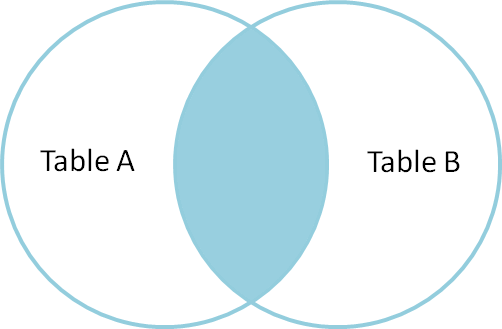
\includegraphics{notebooks/W05. Merging and Joining_files/figure-pdf/cell-33-output-1.png}

}

\end{figure}

(Image from
http://blog.codinghorror.com/a-visual-explanation-of-sql-joins/)

The inner join \emph{only} includes data whose index appears in both
tables. Let's see what that looks like:

\begin{Shaded}
\begin{Highlighting}[]
\NormalTok{df\_joined }\OperatorTok{=}\NormalTok{ df1.merge(df5, left\_index}\OperatorTok{=}\VariableTok{True}\NormalTok{, right\_index}\OperatorTok{=}\VariableTok{True}\NormalTok{)}
\end{Highlighting}
\end{Shaded}

\begin{Shaded}
\begin{Highlighting}[]
\NormalTok{df\_joined}
\end{Highlighting}
\end{Shaded}

\begin{longtable}[]{@{}lllllllll@{}}
\toprule()
& area & population & mean temperature & elevation & annual rainfall &
Mean House Price & median income & walkability score \\
\midrule()
\endhead
London & 5.348823 & 5.486505 & 5.105354 & 3.680852 & 4.487838 & 6.115865
& 5.045850 & 4.932779 \\
Paris & 5.670247 & 5.812321 & 4.076454 & 6.701972 & 3.781139 & 4.115616
& 5.671406 & 6.329527 \\
\bottomrule()
\end{longtable}

Here, we have a couple of arguments specifying the manner of the join -
we have specified that we are joining on the index of the left and right
dataset with the optional ``left\_index=True'' and
``right\_index=True''. Less obviously, the \textbf{left} dataset is df1
(because we're using \emph{df1.merge()} and the \textbf{right} dataset
is df5 (because it appears as an argument in merge(). There's no special
reason it shouldn't be the other way around, but for this function, it
is this way around and we need to remember that when we use it.

\hypertarget{inner-space}{%
\section{Inner Space}\label{inner-space}}

Although we haven't specified it, the merge() function has defaulted to
an inner join (like the diagram above). We can specify how the join is
calculated by changing the text in the optional argument ``how'':

\begin{Shaded}
\begin{Highlighting}[]
\NormalTok{df\_joined }\OperatorTok{=}\NormalTok{ df1.merge(df5, left\_index}\OperatorTok{=}\VariableTok{True}\NormalTok{, right\_index}\OperatorTok{=}\VariableTok{True}\NormalTok{, how}\OperatorTok{=}\StringTok{\textquotesingle{}inner\textquotesingle{}}\NormalTok{)}
\end{Highlighting}
\end{Shaded}

\begin{Shaded}
\begin{Highlighting}[]
\NormalTok{df\_joined}
\end{Highlighting}
\end{Shaded}

\begin{longtable}[]{@{}lllllllll@{}}
\toprule()
& area & population & mean temperature & elevation & annual rainfall &
Mean House Price & median income & walkability score \\
\midrule()
\endhead
London & 5.348823 & 5.486505 & 5.105354 & 3.680852 & 4.487838 & 6.115865
& 5.045850 & 4.932779 \\
Paris & 5.670247 & 5.812321 & 4.076454 & 6.701972 & 3.781139 & 4.115616
& 5.671406 & 6.329527 \\
\bottomrule()
\end{longtable}

\hypertarget{the-future-of-the-left}{%
\section{The Future of The Left}\label{the-future-of-the-left}}

The \emph{left} join includes \textbf{all} rows where the index appears
on the \textbf{left} hand side of the join, and \textbf{any} data which
\textbf{matches} it on the \textbf{right} hand side. If the index
appears on the left but not the right, it will include the data from the
left table, and have blanks for the columns on the right.

\begin{Shaded}
\begin{Highlighting}[]
\NormalTok{data\_path }\OperatorTok{=} \StringTok{"https://s3.eu{-}west{-}2.amazonaws.com/qm2/wk3/left.png"}
\NormalTok{Image(data\_path)}
\end{Highlighting}
\end{Shaded}

\begin{figure}[H]

{\centering 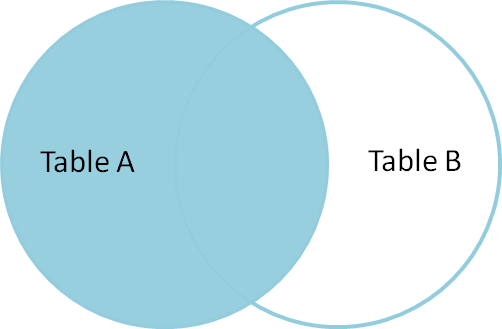
\includegraphics{notebooks/W05. Merging and Joining_files/figure-pdf/cell-38-output-1.png}

}

\end{figure}

What does \emph{this} look like? We will use the \emph{how=`left'}
optional argument to create a left join:

\begin{Shaded}
\begin{Highlighting}[]
\NormalTok{df\_joined }\OperatorTok{=}\NormalTok{ df1.merge(df5, left\_index}\OperatorTok{=}\VariableTok{True}\NormalTok{, right\_index}\OperatorTok{=}\VariableTok{True}\NormalTok{, how}\OperatorTok{=}\StringTok{\textquotesingle{}left\textquotesingle{}}\NormalTok{)}
\end{Highlighting}
\end{Shaded}

\begin{Shaded}
\begin{Highlighting}[]
\NormalTok{df\_joined}
\end{Highlighting}
\end{Shaded}

\begin{longtable}[]{@{}lllllllll@{}}
\toprule()
& area & population & mean temperature & elevation & annual rainfall &
Mean House Price & median income & walkability score \\
\midrule()
\endhead
London & 5.348823 & 5.486505 & 5.105354 & 3.680852 & 4.487838 & 6.115865
& 5.045850 & 4.932779 \\
Paris & 5.670247 & 5.812321 & 4.076454 & 6.701972 & 3.781139 & 4.115616
& 5.671406 & 6.329527 \\
Beijing & 5.707170 & 6.253187 & 3.172944 & 5.131476 & 4.993762 & NaN &
NaN & NaN \\
Medellin & 4.852207 & 3.773460 & 5.652641 & 5.607786 & 4.481264 & NaN &
NaN & NaN \\
Port Elizabeth & 4.320782 & 5.476499 & 5.685651 & 5.537774 & 4.264993 &
NaN & NaN & NaN \\
\bottomrule()
\end{longtable}

As we see, the missing data appears as \textbf{NaN} - Not a Number.

\hypertarget{exercise-13}{%
\section{Exercise:}\label{exercise-13}}

Carry out \emph{right} and \emph{outer} joins on the dataframes df1 and
df5 and explain how they're filtering and joining the data.

\hypertarget{i-am-the-one-and-only}{%
\section{I Am The One and Only}\label{i-am-the-one-and-only}}

So far, we've carried out joins on data which have a \emph{one-to-one}
relationship; data for cities or people. What if our data has a
\emph{one-to-many} correspondence?

\emph{Example:} We want to look at the quality of life in cities (a real
student project from 2014). We have a dataset listing city-level
characteristics for a number of cities in Europe, including the country
each city is in. We also have a dataset listing the GDP, life expectancy
and other indicators for a number of \emph{countries} in Europe. How do
we create a dataframe which, for each city, lists all of the
characteristics of a city and those of its parent country?

We'll be working now with data from the UN, covering information about
cities - real data this time. The UN has some great data, we've taken
some from here and processed it in various ways:

http://data.un.org/Data.aspx?d=POP\&f=tableCode\%3A240

Let's load up data on city population - this set contains data for
2012-2014 inclusive:

\begin{Shaded}
\begin{Highlighting}[]
\NormalTok{data\_path }\OperatorTok{=} \StringTok{"./data/wk3/UN\_Cities\_1214\_population.csv"}

\NormalTok{city\_pop }\OperatorTok{=}\NormalTok{ pd.read\_csv(data\_path, encoding}\OperatorTok{=}\StringTok{\textquotesingle{}latin1\textquotesingle{}}\NormalTok{)}
\end{Highlighting}
\end{Shaded}

\begin{Shaded}
\begin{Highlighting}[]
\NormalTok{city\_pop.head()}
\end{Highlighting}
\end{Shaded}

\begin{longtable}[]{@{}lllllllllll@{}}
\toprule()
& Year & Area & Sex & City & City type & Record Type & Reliability &
Source Year & Value & Value Footnotes \\
\midrule()
\endhead
0 & 2013 & Total & Both Sexes & MARIEHAMN & City proper & Estimate - de
jure & Final figure, complete & 2014 & 11370.0 & NaN \\
1 & 2013 & Total & Male & MARIEHAMN & City proper & Estimate - de jure &
Final figure, complete & 2014 & 5445.0 & NaN \\
2 & 2013 & Total & Female & MARIEHAMN & City proper & Estimate - de jure
& Final figure, complete & 2014 & 5925.0 & NaN \\
3 & 2012 & Total & Both Sexes & MARIEHAMN & City proper & Estimate - de
jure & Final figure, complete & 2013 & 11304.5 & NaN \\
4 & 2012 & Total & Male & MARIEHAMN & City proper & Estimate - de jure &
Final figure, complete & 2013 & 5408.0 & NaN \\
\bottomrule()
\end{longtable}

\hypertarget{exercise-14}{%
\section{Exercise}\label{exercise-14}}

There is a another datafile we downloaded called
\emph{UN\_Cities\_1214\_country.csv}. This is saved to
\emph{./data/wk3/UN\_Cities\_1214\_country.csv} - Load this into a
dataframe called \emph{city\_c} with the city name as the index and view
it; then, using \emph{merge} on city name with city\_pop to create a new
dataframe called \emph{cities}.

\textbf{Hints:} You'll notice that the index \textbf{won't} be the
column you want to merge on in the city\_pop data. What column
\emph{should} you merge on in city\_pop? Which column should you merge
on in city\_c?

The syntax for merging on a \textbf{column} (which is not the index) is
to pass the column name to the optional `left\_on=' or `right\_on='
arguments. And we don't use right\_index=True (or left\_index=True),
depending on which we're using.

So for example: \textbf{df1.merge(df2, left\_on=`Name',
right\_index=True)} would join df1 (on the left) to df2 (on the right),
using the column `Name' on the left (df1) and the index column (whatever
that is) on the right (df2).

\hypertarget{a-footnote-about-footnotes}{%
\section{A footnote about footnotes}\label{a-footnote-about-footnotes}}

Just a quick note - if you look at the primary UN data, you'll see
footnotes which will confuse the hell out of Pandas. I've taken the
footnotes out, but you can use .tail() to see whether there's any junk
in the trunk, and remove it via a text editor.

\hypertarget{clean-data}{%
\section{Clean data}\label{clean-data}}

We need to simplify this data a bit in the following ways:

\begin{enumerate}
\def\labelenumi{\arabic{enumi}.}
\tightlist
\item
  I'm going to focus on one year (2012)
\item
  I'm going to just look at ``Both Sexes'' (not focus on one gender)
\item
  I'm going to get rid of a column of data (the `Value Footnotes'
  column) using the \emph{drop()} method.
\end{enumerate}

\begin{Shaded}
\begin{Highlighting}[]
\NormalTok{cities }\OperatorTok{=}\NormalTok{ cities[cities[}\StringTok{\textquotesingle{}Sex\textquotesingle{}}\NormalTok{]}\OperatorTok{==}\StringTok{\textquotesingle{}Both Sexes\textquotesingle{}}\NormalTok{]}
\NormalTok{cities }\OperatorTok{=}\NormalTok{ cities[cities[}\StringTok{\textquotesingle{}Year\textquotesingle{}}\NormalTok{]}\OperatorTok{==}\DecValTok{2012}\NormalTok{]}
\NormalTok{cities.drop(}\StringTok{\textquotesingle{}Value Footnotes\textquotesingle{}}\NormalTok{, axis}\OperatorTok{=}\DecValTok{1}\NormalTok{, inplace}\OperatorTok{=}\VariableTok{True}\NormalTok{)}
\end{Highlighting}
\end{Shaded}

\begin{verbatim}
NameError: name 'cities' is not defined
\end{verbatim}

\begin{Shaded}
\begin{Highlighting}[]
\NormalTok{cities.head()}
\end{Highlighting}
\end{Shaded}

\hypertarget{extension-in-my-place}{%
\section{Extension: In My Place}\label{extension-in-my-place}}

The command I used to get rid of that column is \emph{cities.drop(`Value
Footnotes', axis=1, inplace=True)}. The syntax is not so complex - the
first argument, \emph{`Value Footnotes'}, is just the name of the
column; the second argument, \emph{axis=1}, tells Pandas to look for a
column to remove (instead of a row which has \emph{axis=0}); the third
and final argument, \emph{inplace=True}, is a command that tells Pandas
to edit \emph{inplace}, i.e.~to edit the dataframe (\emph{cities})
directly. When \emph{inplace} is False (the default), this command does
not directly edit cities, but instead provide an output. So the syntax
for that would be

new\_cities = cities.drop(`Value Footnotes', axis=1)

and new\_cities would be a version of \emph{cities} without the
offending column. This is usually the safer option.

\hypertarget{life-oh-life}{%
\section{Life, Oh Life}\label{life-oh-life}}

The UN also has useful data by country, so let's try and work with some
of that and join it up with our city data. Let's work with Life
Expectancy Data:

http://data.un.org/Data.aspx?d=WDI\&f=Indicator\_Code\%3ASP.DYN.LE00.IN

\begin{Shaded}
\begin{Highlighting}[]
\NormalTok{data\_path }\OperatorTok{=} \StringTok{"./data/wk3/UN\_Life\_all.csv"}
\NormalTok{life }\OperatorTok{=}\NormalTok{ pd.read\_csv(data\_path, index\_col}\OperatorTok{=}\DecValTok{0}\NormalTok{)}
\end{Highlighting}
\end{Shaded}

\begin{Shaded}
\begin{Highlighting}[]
\NormalTok{life.head()}
\end{Highlighting}
\end{Shaded}

\hypertarget{exercise-15}{%
\section{Exercise:}\label{exercise-15}}

In a new cell, clean up the above dataframe by

\begin{itemize}
\tightlist
\item
  removing the ``Value Footnotes'' Column
\item
  use only the most recent data (2012)
\end{itemize}

Let's make it a little clearer what ``Value'' refers to, by renaming the
column. This is one way to do that:

\begin{Shaded}
\begin{Highlighting}[]
\NormalTok{life.rename(columns}\OperatorTok{=}\NormalTok{\{}\StringTok{\textquotesingle{}Value\textquotesingle{}}\NormalTok{:}\StringTok{\textquotesingle{}Life Expectancy\textquotesingle{}}\NormalTok{\}, inplace}\OperatorTok{=}\VariableTok{True}\NormalTok{)}
\end{Highlighting}
\end{Shaded}

\begin{Shaded}
\begin{Highlighting}[]
\NormalTok{life.head()}
\end{Highlighting}
\end{Shaded}

\bookmarksetup{startatroot}

\hypertarget{exercise-16}{%
\chapter{Exercise}\label{exercise-16}}

Now, merge this data with the cities data to show life expectancy for
each city (based on the country it is in), and show the first 5 rows.

How much data was ``missing'' in the merge?

Relabel the City Population column so it's clear what it represents.

\textbf{Extension:} Plot population against life expectancy. Use plot's
\emph{optional arguments} to specify the x column, y column, and that
kind=`scatter'.

\textbf{Don't forget to include a title and axis labels!}

How does London fit in this trend? What are the problems with doing
this?

\hypertarget{recap-joins}{%
\section{Recap: Joins}\label{recap-joins}}

Pandas has \textbf{four} join methods:

\begin{verbatim}
- Left Join: use **only** keys from **left** DataFrame. SQL: [left outer join](http://goo.gl/JICveI)
- Right Join: use **only** keys from **right** DataFrame. SQL: [right outer join](http://goo.gl/TrrHjQ)
- Outer Join: use union of **keys from both** DataFrames. SQL: [full outer join](http://goo.gl/bVRqO8)
- Inner Join: use **intersection of keys** from both DataFrames. SQL: [inner join](http://goo.gl/Cf1MF8)
\end{verbatim}

\bookmarksetup{startatroot}

\hypertarget{group-presentations}{%
\chapter{Group Presentations}\label{group-presentations}}

\bookmarksetup{startatroot}

\hypertarget{distributions-and-basic-statistics}{%
\chapter{Distributions and Basic
Statistics}\label{distributions-and-basic-statistics}}

\hypertarget{workshop-7-open-in-colab}{%
\section[\emph{Workshop 7} ]{\texorpdfstring{\emph{Workshop 7}
\href{https://colab.research.google.com/github/oballinger/QM2/blob/main/notebooks/W07.\%20Distributions\%20and\%20Basic\%20Statistics.ipynb}{\protect
\includegraphics{notebooks/../colab-badge.png}}}{Workshop 7 Open In Colab}}\label{workshop-7-open-in-colab}}

For the rest of this course, we'll be working with data from the U.S.
Census \href{https://www.census.gov/programs-surveys/cps.html}{Current
Population Survey (CPS)}.

\hypertarget{aims-3}{%
\subsection{Aims:}\label{aims-3}}

\begin{itemize}
\item
  Choosing appropriate summary statistics for varying distributions
\item
  Understanding:

  \begin{itemize}
  \tightlist
  \item
    The nature of our dataset, including potential bias
  \item
    How to generate summary statistics for our dataset
  \item
    The distribution of different variables
  \item
    The intuition behind the Central Limit Theorem
  \end{itemize}
\end{itemize}

\hypertarget{getting-started-1}{%
\section{Getting Started}\label{getting-started-1}}

\hypertarget{first-things-first-bias}{%
\subsection{First Things First: Bias}\label{first-things-first-bias}}

Once we've acquired a dataset, the first step is \emph{always} to
develop an understanding of where the data has come from. For this
dataset, use the following
\href{https://www.census.gov/programs-surveys/cps/technical-documentation/methodology.html}{documentation
page} to answer the questions below:

\begin{enumerate}
\def\labelenumi{\arabic{enumi})}
\tightlist
\item
  What is the population of interest?
\item
  What was the sampling strategy?
\item
  What are potential sources of selection bias?
\end{enumerate}

I'll start by importing the libraries I need: matplotlib (for graphs),
pandas (for data), numpy (for maths) and random (for generating random
numbers):

\begin{Shaded}
\begin{Highlighting}[]
\CommentTok{\#This is a comment {-} python does not try to execute it}

\CommentTok{\#This tells python to draw the graphs "inline" {-} in the notebook}
\OperatorTok{\%}\NormalTok{matplotlib inline  }
\ImportTok{import}\NormalTok{ matplotlib.pyplot }\ImportTok{as}\NormalTok{ plt}
\ImportTok{from}\NormalTok{ scipy.stats }\ImportTok{import}\NormalTok{ norm}
\ImportTok{import}\NormalTok{ statistics}

\ImportTok{import}\NormalTok{ pylab}
\ImportTok{import}\NormalTok{ pandas }\ImportTok{as}\NormalTok{ pd}
\ImportTok{import}\NormalTok{ numpy }\ImportTok{as}\NormalTok{ np}
\CommentTok{\# make the plots (graphs) a little wider by default}
\NormalTok{pylab.rcParams[}\StringTok{\textquotesingle{}figure.figsize\textquotesingle{}}\NormalTok{] }\OperatorTok{=}\NormalTok{ (}\FloatTok{10.}\NormalTok{, }\FloatTok{8.}\NormalTok{)}
\end{Highlighting}
\end{Shaded}

\hypertarget{section}{%
\section{}\label{section}}

The first thing to notice is that I'm using an \textbf{alias} for
matplotlib.pyplot - it's a bit ungainly, so I'm using ``plt'' in its
place. That's just to make the coding easier. I'll do the same for some
of the other libraries as we go through - this isn't necessary, but
online examples frequently use ``pd'' for ``pandas'' (for example), so
it can be useful to use these. The way it works is pretty simple - now
I've used ``plt'' as my alias for matplotlib.pyplot, I can just say
``plt.\emph{command()}'' whenever I need to use functions from that
library.

Now that I've imported the libraries I'm going to be using, I'm ready to
import the data:

\begin{Shaded}
\begin{Highlighting}[]
\NormalTok{df}\OperatorTok{=}\NormalTok{pd.read\_csv(}\StringTok{\textquotesingle{}./data/wk7/cps.csv\textquotesingle{}}\NormalTok{)}
\NormalTok{df.head()}
\end{Highlighting}
\end{Shaded}

\begin{longtable}[]{@{}llllllllllll@{}}
\toprule()
& year & state & age & sex & race & sch & ind & union & incwage &
realhrwage & occupation \\
\midrule()
\endhead
0 & 1990 & 36 & 58 & 1 & 3 & 12.0 & 871 & 0.0 & 14200.0 & 12.269874 &
Office and Admin Support \\
1 & 2009 & 5 & 28 & 1 & 1 & 12.0 & 8660 & 1.0 & 17680.0 & 8.635149 &
Office and Admin Support \\
2 & 1990 & 36 & 37 & 1 & 1 & 14.0 & 380 & 1.0 & 28000.0 & 21.169851 &
. \\
3 & 1990 & 6 & 34 & 1 & 1 & 18.0 & 740 & 1.0 & 27500.0 & 20.447746 &
Computer and Math Technicians \\
4 & 1981 & 51 & 38 & 1 & 4 & 13.0 & 798 & NaN & 17000.0 & 18.892282 &
Managers \\
\bottomrule()
\end{longtable}

Our dataframe has 10 columns:

\begin{enumerate}
\def\labelenumi{\arabic{enumi}.}
\tightlist
\item
  \emph{year}: Survey year
\item
  \emph{age}: the person's age
\item
  \emph{sex}: the person's sex

  \begin{itemize}
  \tightlist
  \item
    1=male
  \item
    2=female
  \end{itemize}
\item
  \emph{race}: the person's race

  \begin{itemize}
  \tightlist
  \item
    White non hispanic=1
  \item
    Black non hispanic=2
  \item
    Hispanic=3
  \item
    Other non hispanic=4)
  \end{itemize}
\item
  \emph{sch}: Educational attainment

  \begin{itemize}
  \tightlist
  \item
    None = 0,
  \item
    Grades 1-12 = 1-12
  \item
    Some University = 13,
  \item
    Associate's degree = 14,
  \item
    BA = 16
  \item
    Advanced Degree = 18
  \end{itemize}
\item
  \emph{union}: Union membership

  \begin{itemize}
  \tightlist
  \item
    N/A = 0,
  \item
    No union coverage = 1,
  \item
    Member of labor union=2,
  \item
    Covered by union but not a member=3
  \end{itemize}
\item
  \emph{incwage}: Wage and salary income
\item
  \emph{realhrwage}: Real Hourly Wage
\item
  \emph{occupation}: Occupation
\item
  \emph{ind}:
  \href{https://www.census.gov/naics/?58967?yearbck=2002}{industry code}
\end{enumerate}

Based on the data

\hypertarget{summary-statistics}{%
\section{Summary Statistics}\label{summary-statistics}}

After thinking about the origins of our dataset and loading it into
python, the next step is to generate summary statistics. This is vital
for us to better understand our data. Pandas has a useful function,
\texttt{describe}, which will generate summary statistics for all
numerical variables in our entire dataframe:

\begin{Shaded}
\begin{Highlighting}[]
\NormalTok{df.describe()}
\end{Highlighting}
\end{Shaded}

\begin{longtable}[]{@{}lllllllllll@{}}
\toprule()
& year & state & age & sex & race & sch & ind & union & incwage &
realhrwage \\
\midrule()
\endhead
count & 344287.000000 & 344287.000000 & 344287.000000 & 344287.000000 &
344287.000000 & 344287.000000 & 344287.000000 & 301908.000000 &
3.442870e+05 & 344287.000000 \\
mean & 2002.599122 & 28.121004 & 41.734364 & 1.489057 & 1.570077 &
13.498057 & 4235.846009 & 0.221505 & 3.976170e+04 & 22.886629 \\
std & 10.831555 & 15.818556 & 10.415874 & 0.499881 & 0.952252 & 2.799038
& 3468.163157 & 0.499690 & 4.529758e+04 & 506.489695 \\
min & 1981.000000 & 1.000000 & 25.000000 & 1.000000 & 1.000000 &
0.000000 & 10.000000 & 0.000000 & 1.500000e+01 & 2.000000 \\
25\% & 1990.000000 & 13.000000 & 33.000000 & 1.000000 & 1.000000 &
12.000000 & 760.000000 & 0.000000 & 1.670000e+04 & 11.723004 \\
50\% & 2007.000000 & 28.000000 & 41.000000 & 1.000000 & 1.000000 &
13.000000 & 4270.000000 & 0.000000 & 3.000000e+04 & 17.698591 \\
75\% & 2011.000000 & 41.000000 & 50.000000 & 2.000000 & 2.000000 &
16.000000 & 7860.000000 & 0.000000 & 5.000000e+04 & 26.442308 \\
max & 2013.000000 & 56.000000 & 64.000000 & 2.000000 & 4.000000 &
18.000000 & 9590.000000 & 3.000000 & 1.259999e+06 & 294610.968750 \\
\bottomrule()
\end{longtable}

\texttt{describe} returns a dataframe with the same columns as the
source dataframe. For numeric data, the result's index will include
count, mean, std, min, max as well as lower, 50 and upper percentiles.
By default the lower percentile is 25 and the upper percentile is 75.
The 50 percentile is the same as the median. Given these summary
statistics, answer the following questions:

\begin{enumerate}
\def\labelenumi{\arabic{enumi})}
\tightlist
\item
  what is the median hourly wage?
\item
  what is the average age?
\item
  are there more men or women?
\item
  intepret the mean of the ``race'' column.
\end{enumerate}

The answer to the last question should provoke some futher thought; the
race column is categorical, but because it contains numbers it's being
treated as numerical. The mean of a categorical variable is meaningless;
For object data (e.g.~categories, strings or timestamps), the result's
index will include count, unique, top, and freq. The top is the most
common value. The freq is the most common value's frequency. Timestamps
also include the first and last items.

Let's convert the race column from a numerical variable into a
categorical one, and try \texttt{describe} once again:

\begin{Shaded}
\begin{Highlighting}[]
\NormalTok{df.dtypes}
\end{Highlighting}
\end{Shaded}

\begin{verbatim}
year            int64
state           int64
age             int64
sex             int64
race            int64
sch           float64
ind             int64
union         float64
incwage       float64
realhrwage    float64
occupation     object
dtype: object
\end{verbatim}

\begin{Shaded}
\begin{Highlighting}[]
\NormalTok{df[}\StringTok{\textquotesingle{}race\textquotesingle{}}\NormalTok{]}\OperatorTok{=}\NormalTok{df[}\StringTok{\textquotesingle{}race\textquotesingle{}}\NormalTok{].astype(}\StringTok{\textquotesingle{}category\textquotesingle{}}\NormalTok{)}
\NormalTok{df[}\StringTok{\textquotesingle{}race\textquotesingle{}}\NormalTok{].describe()}
\end{Highlighting}
\end{Shaded}

\begin{verbatim}
count     344287
unique         4
top            1
freq      240382
Name: race, dtype: int64
\end{verbatim}

what other variables are categorical? Convert them to categorical and
describe. What is the most common occupation in this dataset?

\begin{Shaded}
\begin{Highlighting}[]
\CommentTok{\# convert the variables to categorical and describe}
\end{Highlighting}
\end{Shaded}

These statistics are useful, but suppose we want detailed counts of the
number of individuals in each category; For this, we can use the
\texttt{groupby} function, with the \texttt{.size()} operator which
simply counts the number of rows in each category.

\begin{Shaded}
\begin{Highlighting}[]
\NormalTok{occupations}\OperatorTok{=}\NormalTok{ df.groupby(}\StringTok{\textquotesingle{}occupation\textquotesingle{}}\NormalTok{).size()}
\NormalTok{occupations.sort\_values(ascending}\OperatorTok{=}\VariableTok{False}\NormalTok{)}
\end{Highlighting}
\end{Shaded}

\begin{verbatim}
occupation
.                                         132708
Office and Admin Support                   50635
Managers                                   35696
Consruction, Extraction, Installation      30579
Production                                 29732
Transportation and materials moving        21277
Computer and Math Technicians               8602
Protective Service adj_occupations          7809
financial Operators                         7702
Business Operators                          7327
Community and Social Workers                6025
Lawyers, Judges,Physicans and dentists      3835
Farming, Fishing & Forestry                 2360
dtype: int64
\end{verbatim}

What is the most common profession?

\bookmarksetup{startatroot}

\hypertarget{distributions}{%
\chapter{Distributions}\label{distributions}}

Now that we've cleaned our data up, let's have a closer look at the
\emph{distribution} of our data. The best way to do this is using a
histogram. Let's start by looking at the distribution of the
\texttt{incwage} variable:

\begin{Shaded}
\begin{Highlighting}[]
\NormalTok{df}\OperatorTok{=}\NormalTok{df[df[}\StringTok{\textquotesingle{}year\textquotesingle{}}\NormalTok{]}\OperatorTok{==}\DecValTok{2013}\NormalTok{]}

\NormalTok{plt.hist(df[}\StringTok{\textquotesingle{}incwage\textquotesingle{}}\NormalTok{])}
\NormalTok{plt.show()}
\end{Highlighting}
\end{Shaded}

\begin{figure}[H]

{\centering 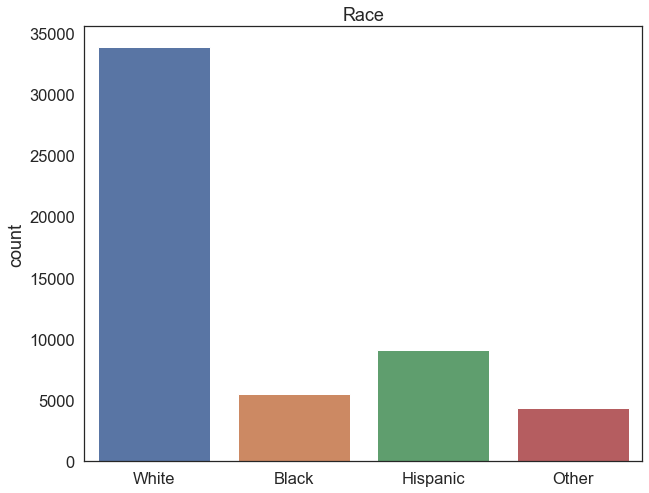
\includegraphics{notebooks/W07. Distributions and Basic Statistics_files/figure-pdf/cell-9-output-1.png}

}

\end{figure}

\begin{Shaded}
\begin{Highlighting}[]
\NormalTok{income}\OperatorTok{=}\NormalTok{df[}\StringTok{\textquotesingle{}incwage\textquotesingle{}}\NormalTok{]}\OperatorTok{/}\DecValTok{1000}

\NormalTok{plt.hist(income, bins}\OperatorTok{=}\DecValTok{100}\NormalTok{, edgecolor}\OperatorTok{=}\StringTok{\textquotesingle{}white\textquotesingle{}}\NormalTok{)}
\NormalTok{plt.xlabel(}\StringTok{\textquotesingle{}Income ($, thousands\textquotesingle{}}\NormalTok{)}
\NormalTok{plt.title(}\StringTok{"U.S. Income Distributon, 2013"}\NormalTok{)}

\NormalTok{plt.show()}
\end{Highlighting}
\end{Shaded}

\begin{figure}[H]

{\centering 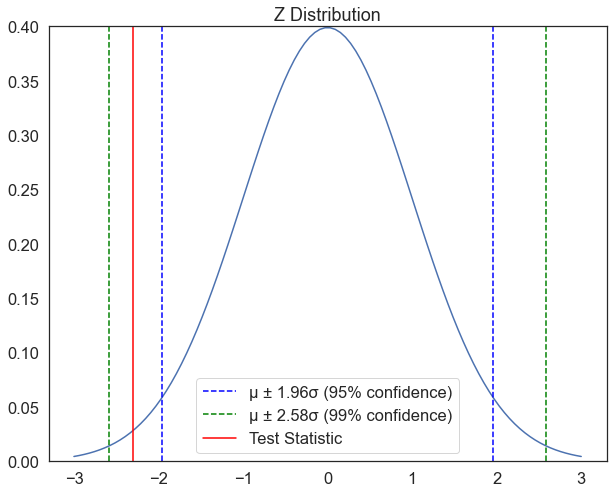
\includegraphics{notebooks/W07. Distributions and Basic Statistics_files/figure-pdf/cell-10-output-1.png}

}

\end{figure}

\begin{Shaded}
\begin{Highlighting}[]
\NormalTok{inc\_summary}\OperatorTok{=}\NormalTok{income.describe()}
\BuiltInTok{print}\NormalTok{(inc\_summary[[}\StringTok{\textquotesingle{}mean\textquotesingle{}}\NormalTok{,}\StringTok{\textquotesingle{}50\%\textquotesingle{}}\NormalTok{,}\StringTok{\textquotesingle{}std\textquotesingle{}}\NormalTok{]])}

\NormalTok{plt.hist(income, bins}\OperatorTok{=}\DecValTok{100}\NormalTok{, edgecolor}\OperatorTok{=}\StringTok{\textquotesingle{}white\textquotesingle{}}\NormalTok{)}
\NormalTok{plt.axvline(inc\_summary[}\StringTok{\textquotesingle{}mean\textquotesingle{}}\NormalTok{], color}\OperatorTok{=}\StringTok{\textquotesingle{}red\textquotesingle{}}\NormalTok{, linestyle}\OperatorTok{=}\StringTok{\textquotesingle{}dashed\textquotesingle{}}\NormalTok{, linewidth}\OperatorTok{=}\DecValTok{1}\NormalTok{,label}\OperatorTok{=}\StringTok{\textquotesingle{}Mean\textquotesingle{}}\NormalTok{)}
\NormalTok{plt.axvline(inc\_summary[}\StringTok{\textquotesingle{}50\%\textquotesingle{}}\NormalTok{], color}\OperatorTok{=}\StringTok{\textquotesingle{}black\textquotesingle{}}\NormalTok{, linestyle}\OperatorTok{=}\StringTok{\textquotesingle{}dashed\textquotesingle{}}\NormalTok{, linewidth}\OperatorTok{=}\DecValTok{1}\NormalTok{, label}\OperatorTok{=}\StringTok{\textquotesingle{}Median\textquotesingle{}}\NormalTok{)}

\NormalTok{plt.legend()}
\NormalTok{plt.xlabel(}\StringTok{\textquotesingle{}Income ($, thousands\textquotesingle{}}\NormalTok{)}
\NormalTok{plt.title(}\StringTok{"U.S. Income Distributon, 2013"}\NormalTok{)}
\NormalTok{plt.xlim(}\DecValTok{0}\NormalTok{,}\DecValTok{250}\NormalTok{)}
\NormalTok{plt.show()}
\end{Highlighting}
\end{Shaded}

\begin{verbatim}
mean    51.821863
50%     40.000000
std     60.163449
Name: incwage, dtype: float64
\end{verbatim}

\begin{figure}[H]

{\centering 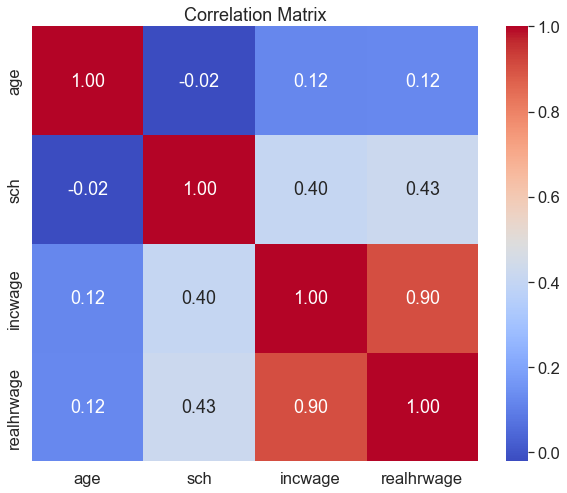
\includegraphics{notebooks/W07. Distributions and Basic Statistics_files/figure-pdf/cell-11-output-2.png}

}

\end{figure}

\begin{Shaded}
\begin{Highlighting}[]
\KeywordTok{def}\NormalTok{ plot\_histogram(variable, bins, xlab, title):}
\NormalTok{    summary}\OperatorTok{=}\NormalTok{variable.describe()}
\NormalTok{    plt.hist(variable, bins}\OperatorTok{=}\NormalTok{bins,edgecolor}\OperatorTok{=}\StringTok{\textquotesingle{}white\textquotesingle{}}\NormalTok{, density}\OperatorTok{=}\VariableTok{True}\NormalTok{)}
\NormalTok{    plt.axvline(summary[}\StringTok{\textquotesingle{}mean\textquotesingle{}}\NormalTok{], color}\OperatorTok{=}\StringTok{\textquotesingle{}red\textquotesingle{}}\NormalTok{, linestyle}\OperatorTok{=}\StringTok{\textquotesingle{}dashed\textquotesingle{}}\NormalTok{, linewidth}\OperatorTok{=}\DecValTok{1}\NormalTok{,label}\OperatorTok{=}\StringTok{\textquotesingle{}Mean \textquotesingle{}}\OperatorTok{+}\BuiltInTok{str}\NormalTok{(}\BuiltInTok{round}\NormalTok{(summary[}\StringTok{\textquotesingle{}mean\textquotesingle{}}\NormalTok{],}\DecValTok{2}\NormalTok{)))}
\NormalTok{    plt.axvline(summary[}\StringTok{\textquotesingle{}50\%\textquotesingle{}}\NormalTok{], color}\OperatorTok{=}\StringTok{\textquotesingle{}black\textquotesingle{}}\NormalTok{, linestyle}\OperatorTok{=}\StringTok{\textquotesingle{}dashed\textquotesingle{}}\NormalTok{, linewidth}\OperatorTok{=}\DecValTok{1}\NormalTok{, label}\OperatorTok{=}\StringTok{\textquotesingle{}Median \textquotesingle{}}\OperatorTok{+}\BuiltInTok{str}\NormalTok{(}\BuiltInTok{round}\NormalTok{(summary[}\StringTok{\textquotesingle{}50\%\textquotesingle{}}\NormalTok{],}\DecValTok{2}\NormalTok{)))}

\NormalTok{    plt.legend()}
\NormalTok{    plt.xlabel(xlab)}
\NormalTok{    plt.title(title)}
\NormalTok{    plt.show()}

\NormalTok{plot\_histogram(df[}\StringTok{\textquotesingle{}incwage\textquotesingle{}}\NormalTok{]}\OperatorTok{/}\DecValTok{1000}\NormalTok{, bins}\OperatorTok{=}\DecValTok{100}\NormalTok{, xlab}\OperatorTok{=}\StringTok{\textquotesingle{}Income ($, 000)\textquotesingle{}}\NormalTok{,title}\OperatorTok{=}\StringTok{\textquotesingle{}U.S. Income Distribution, 2013\textquotesingle{}}\NormalTok{)}
\end{Highlighting}
\end{Shaded}

\begin{figure}[H]

{\centering 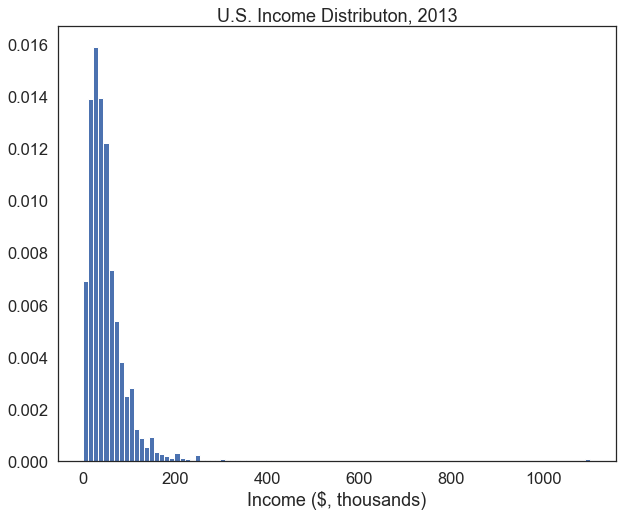
\includegraphics{notebooks/W07. Distributions and Basic Statistics_files/figure-pdf/cell-12-output-1.png}

}

\end{figure}

\begin{Shaded}
\begin{Highlighting}[]
\NormalTok{plot\_histogram(df[}\StringTok{\textquotesingle{}age\textquotesingle{}}\NormalTok{], bins}\OperatorTok{=}\DecValTok{20}\NormalTok{, xlab}\OperatorTok{=}\StringTok{\textquotesingle{}Age\textquotesingle{}}\NormalTok{,title}\OperatorTok{=}\StringTok{\textquotesingle{}U.S. Age Distribution, 2013\textquotesingle{}}\NormalTok{)}
\end{Highlighting}
\end{Shaded}

\begin{figure}[H]

{\centering 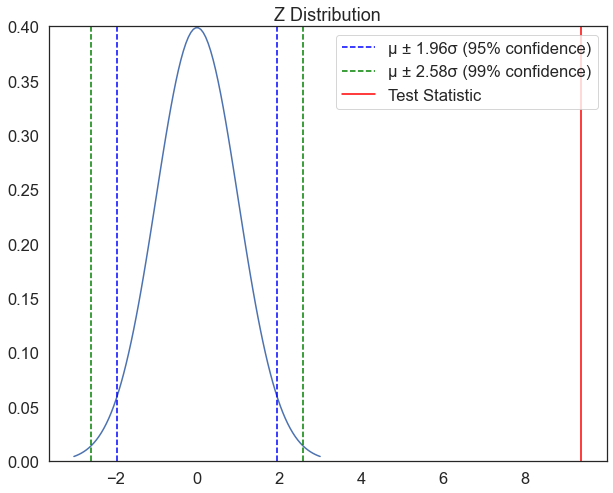
\includegraphics{notebooks/W07. Distributions and Basic Statistics_files/figure-pdf/cell-13-output-1.png}

}

\end{figure}

\begin{Shaded}
\begin{Highlighting}[]
\NormalTok{mu, se}\OperatorTok{=} \DecValTok{0}\NormalTok{, }\DecValTok{1}
\NormalTok{x }\OperatorTok{=}\NormalTok{ np.linspace(mu }\OperatorTok{{-}} \DecValTok{3}\OperatorTok{*}\NormalTok{se, mu }\OperatorTok{+} \DecValTok{3}\OperatorTok{*}\NormalTok{se, }\DecValTok{100}\NormalTok{)}
\NormalTok{plt.plot(x, norm.pdf(x, mu, se))}
\NormalTok{plt.axvline(mu, color}\OperatorTok{=}\StringTok{\textquotesingle{}black\textquotesingle{}}\NormalTok{, linestyle}\OperatorTok{=}\StringTok{\textquotesingle{}solid\textquotesingle{}}\NormalTok{, linewidth}\OperatorTok{=}\DecValTok{1}\NormalTok{,label}\OperatorTok{=}\StringTok{\textquotesingle{}µ\textquotesingle{}}\NormalTok{)}
\NormalTok{plt.axvline(mu}\OperatorTok{{-}}\NormalTok{se}\OperatorTok{*}\DecValTok{2}\NormalTok{, color}\OperatorTok{=}\StringTok{\textquotesingle{}black\textquotesingle{}}\NormalTok{, linestyle}\OperatorTok{=}\StringTok{\textquotesingle{}dashed\textquotesingle{}}\NormalTok{, linewidth}\OperatorTok{=}\FloatTok{1.5}\NormalTok{,label}\OperatorTok{=}\StringTok{\textquotesingle{}µ ± 2σ\textquotesingle{}}\NormalTok{)}
\NormalTok{plt.axvline(mu}\OperatorTok{+}\NormalTok{se}\OperatorTok{*}\DecValTok{2}\NormalTok{, color}\OperatorTok{=}\StringTok{\textquotesingle{}black\textquotesingle{}}\NormalTok{, linestyle}\OperatorTok{=}\StringTok{\textquotesingle{}dashed\textquotesingle{}}\NormalTok{, linewidth}\OperatorTok{=}\FloatTok{1.5}\NormalTok{)}
\NormalTok{plt.legend()}
\NormalTok{plt.show()}
\end{Highlighting}
\end{Shaded}

\begin{figure}[H]

{\centering 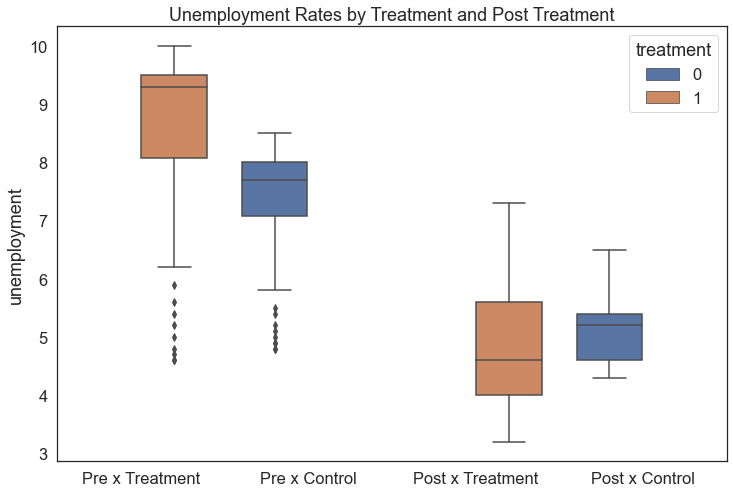
\includegraphics{notebooks/W07. Distributions and Basic Statistics_files/figure-pdf/cell-15-output-1.png}

}

\end{figure}

\begin{Shaded}
\begin{Highlighting}[]
\KeywordTok{def}\NormalTok{ plot\_sample\_means(var, xlab, sample\_size):}

    \CommentTok{\#create an empty list to store sample means}
\NormalTok{    sample\_means}\OperatorTok{=}\NormalTok{[]}

    \CommentTok{\# loop 10,000 times.}
    \ControlFlowTok{for}\NormalTok{ i }\KeywordTok{in} \BuiltInTok{range}\NormalTok{(}\DecValTok{0}\NormalTok{,}\DecValTok{10000}\NormalTok{):}
        \CommentTok{\# for each iteration, draw a sample of the size specified by the "sample\_size" parameter}
\NormalTok{        sample}\OperatorTok{=}\NormalTok{var.sample(sample\_size, replace}\OperatorTok{=}\VariableTok{True}\NormalTok{)}
        \CommentTok{\# calculate the mean, and append it to the list of sample means. }
\NormalTok{        sample\_mean}\OperatorTok{=}\NormalTok{sample.mean()}
\NormalTok{        sample\_means.append(sample\_mean)}
    
    \CommentTok{\# now, plot a histogram }
\NormalTok{    plt.hist(sample\_means, bins}\OperatorTok{=}\BuiltInTok{int}\NormalTok{(}\DecValTok{30}\NormalTok{), color}\OperatorTok{=} \StringTok{\textquotesingle{}green\textquotesingle{}}\NormalTok{, edgecolor}\OperatorTok{=}\StringTok{\textquotesingle{}white\textquotesingle{}}\NormalTok{, density}\OperatorTok{=}\VariableTok{True}\NormalTok{)}
    
    \CommentTok{\# fit a normal distribution to the data }
\NormalTok{    mu, se }\OperatorTok{=}\NormalTok{ norm.fit(sample\_means)}
\NormalTok{    xmin, xmax }\OperatorTok{=}\NormalTok{ plt.xlim()}
\NormalTok{    x }\OperatorTok{=}\NormalTok{ np.linspace(xmin, xmax, }\DecValTok{100}\NormalTok{)}
\NormalTok{    p }\OperatorTok{=}\NormalTok{ norm.pdf(x, mu, se) }
\NormalTok{    plt.plot(x, p, }\StringTok{\textquotesingle{}k\textquotesingle{}}\NormalTok{, linewidth}\OperatorTok{=}\DecValTok{2}\NormalTok{)}

    \CommentTok{\# calculate the difference between the mean of the sample means }
\NormalTok{    diff}\OperatorTok{=}\BuiltInTok{abs}\NormalTok{(mu}\OperatorTok{{-}}\NormalTok{var.mean())}
    
    \CommentTok{\# add droplines, labels, title, legend, and limit the x{-}axis range to 3 standard deviations from the mean on either side.}
\NormalTok{    plt.axvline(mu, color}\OperatorTok{=}\StringTok{\textquotesingle{}black\textquotesingle{}}\NormalTok{, linestyle}\OperatorTok{=}\StringTok{\textquotesingle{}dashed\textquotesingle{}}\NormalTok{, linewidth}\OperatorTok{=}\DecValTok{1}\NormalTok{,label}\OperatorTok{=}\StringTok{\textquotesingle{}µx̄ {-} µ= \textquotesingle{}}\OperatorTok{+}\BuiltInTok{str}\NormalTok{(}\BuiltInTok{round}\NormalTok{(diff, }\DecValTok{3}\NormalTok{)))}
\NormalTok{    plt.axvline(mu}\OperatorTok{{-}}\NormalTok{se}\OperatorTok{*}\DecValTok{2}\NormalTok{, color}\OperatorTok{=}\StringTok{\textquotesingle{}black\textquotesingle{}}\NormalTok{, linestyle}\OperatorTok{=}\StringTok{\textquotesingle{}dashed\textquotesingle{}}\NormalTok{, linewidth}\OperatorTok{=}\FloatTok{1.5}\NormalTok{,label}\OperatorTok{=}\StringTok{\textquotesingle{}µ ± 2σ\textquotesingle{}}\NormalTok{)}
\NormalTok{    plt.axvline(mu}\OperatorTok{+}\NormalTok{se}\OperatorTok{*}\DecValTok{2}\NormalTok{, color}\OperatorTok{=}\StringTok{\textquotesingle{}black\textquotesingle{}}\NormalTok{, linestyle}\OperatorTok{=}\StringTok{\textquotesingle{}dashed\textquotesingle{}}\NormalTok{, linewidth}\OperatorTok{=}\FloatTok{1.5}\NormalTok{)}
\NormalTok{    plt.legend()}
\NormalTok{    plt.xlabel(xlab)    }
\NormalTok{    plt.title(}\StringTok{\textquotesingle{}Distribution of Sample Means (n=}\SpecialCharTok{\{\}}\StringTok{)\textquotesingle{}}\NormalTok{.}\BuiltInTok{format}\NormalTok{(sample\_size))}
\NormalTok{    plt.xlim(mu}\OperatorTok{{-}}\NormalTok{se}\OperatorTok{*}\DecValTok{3}\NormalTok{, mu}\OperatorTok{+}\NormalTok{se}\OperatorTok{*}\DecValTok{3}\NormalTok{)}
\NormalTok{    plt.show()  }
\end{Highlighting}
\end{Shaded}

\begin{Shaded}
\begin{Highlighting}[]
\NormalTok{plot\_sample\_means(income, xlab}\OperatorTok{=}\StringTok{\textquotesingle{}Income, ($, 000)\textquotesingle{}}\NormalTok{, sample\_size}\OperatorTok{=}\DecValTok{2}\NormalTok{)}
\end{Highlighting}
\end{Shaded}

\begin{figure}[H]

{\centering 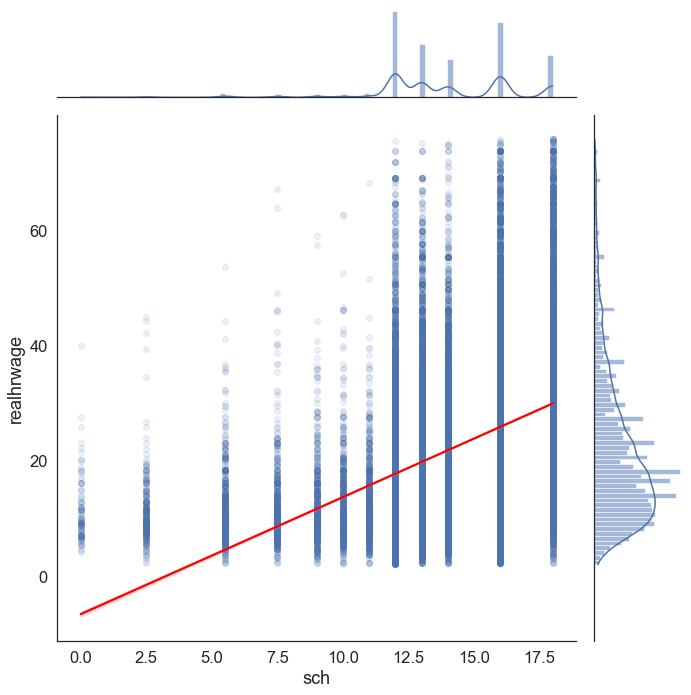
\includegraphics{notebooks/W07. Distributions and Basic Statistics_files/figure-pdf/cell-17-output-1.png}

}

\end{figure}

\begin{Shaded}
\begin{Highlighting}[]
\NormalTok{plot\_sample\_means(df[}\StringTok{\textquotesingle{}union\textquotesingle{}}\NormalTok{], xlab}\OperatorTok{=}\StringTok{\textquotesingle{}Income, ($, 000)\textquotesingle{}}\NormalTok{, sample\_size}\OperatorTok{=}\DecValTok{1000}\NormalTok{)}
\end{Highlighting}
\end{Shaded}

\begin{figure}[H]

{\centering 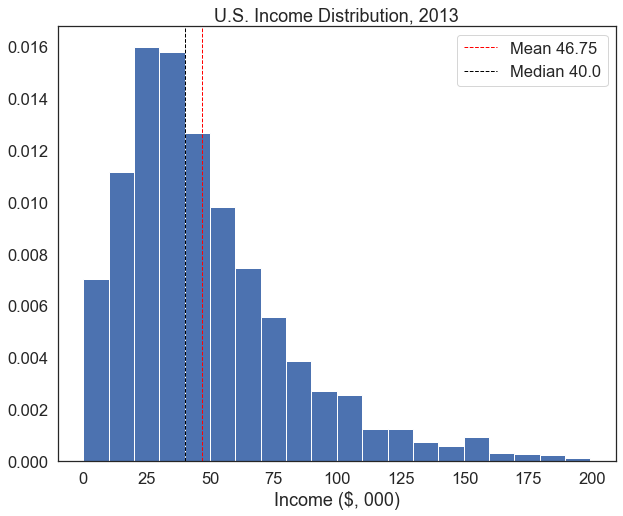
\includegraphics{notebooks/W07. Distributions and Basic Statistics_files/figure-pdf/cell-18-output-1.png}

}

\end{figure}

\bookmarksetup{startatroot}

\hypertarget{exercise-counting-heads}{%
\chapter{Exercise: counting heads}\label{exercise-counting-heads}}

By modifying variables in the code above, create and plot a distribution
of heights for \emph{men} in the USA. Use of wikipedia and the internet
is allowed. Social media is not.

How many men in America are average height? (Hint: think about the
``sample'' variable)

\emph{Extension:} How many men in the USA are within 7cm of the mean?

\bookmarksetup{startatroot}

\hypertarget{in-the-bin}{%
\chapter{In the bin}\label{in-the-bin}}

Slightly more subtly, the bin size might affect our answers to some of
these questions. In order to create a distribution, we need to
\emph{bin} data to create the graph that we've created - a
\emph{histogram} which we expect to reflect the probability mass
function. If I give you a string of heights (1.1, 1.5, 1.6, 1.2, 1.8,
1.4, 1.0, 1.55, 1.74, etc) you can probably see that they cluster around
1.5 or thereabouts, but to graph them as a histogram, you need to choose
a bin size and range. Let's say we choose 10 bins, starting at 1m and
each bin is 0.1m bigger. So if the height h is 1.0 \(\leq\) h
\textless{} 1.1, it goes into the first bin, if 1.1 \(\leq\) h
\textless{} 1.2 in the second and so on. For this data, we'd see one
entry in the first bin, one in the second, a few around the middle and
only one in the higher echelons.

This is pretty basic and you're probably familiar with it. But you need
to choose the number of bins appropriately for the data set - and that's
very sensitive to the number of samples you have.

\bookmarksetup{startatroot}

\hypertarget{exercise-keep-gaussians-tidy}{%
\chapter{Exercise: Keep Gaussians
Tidy}\label{exercise-keep-gaussians-tidy}}

In the above code, increase the number of bins to 1000 - what do you
notice?

Reduce the number of bins to 10 - what happens now? What's causing this
effect?

Reduce the number of samples to 1000. What affect does this have on the
histogram?

How can you use this information for plotting and binning data?

\emph{Extension}: to find more about the function used to sample these
random numbers above, take a look at the Python documentation:
http://docs.scipy.org/doc/numpy/reference/generated/numpy.random.randn.html)

\bookmarksetup{startatroot}

\hypertarget{some-normal-behaviours}{%
\chapter{Some Normal Behaviours}\label{some-normal-behaviours}}

Let's look at the mean and standard deviation on the graph. We can
calculate the mean and standard deviation of our (synthetic) dataset a
by using the np.mean() and np.std() methods.

Recall that the . notation means we're using a method from ``inside''
the numpy library.

\begin{Shaded}
\begin{Highlighting}[]
\CommentTok{\#as we did before...}
\NormalTok{plt.hist(heights, bins, histtype}\OperatorTok{=}\StringTok{\textquotesingle{}step\textquotesingle{}}\NormalTok{)}
\CommentTok{\#draw the mean}
\NormalTok{plt.axvline(numpy.mean(heights), color }\OperatorTok{=} \StringTok{\textquotesingle{}r\textquotesingle{}}\NormalTok{)}
\NormalTok{sd }\OperatorTok{=}\NormalTok{ numpy.std(heights)}
\CommentTok{\#draw mean + one s.d.}
\NormalTok{plt.axvline(numpy.mean(heights) }\OperatorTok{+}\NormalTok{ sd, color}\OperatorTok{=}\StringTok{\textquotesingle{}k\textquotesingle{}}\NormalTok{)}
\CommentTok{\#draw mean {-} one s.d.}
\NormalTok{plt.axvline(numpy.mean(heights) }\OperatorTok{{-}}\NormalTok{ sd, color }\OperatorTok{=} \StringTok{\textquotesingle{}k\textquotesingle{}}\NormalTok{)}
\NormalTok{plt.xlabel(}\StringTok{\textquotesingle{}Height [cm]\textquotesingle{}}\NormalTok{)}
\NormalTok{plt.ylabel(}\StringTok{\textquotesingle{}Frequency\textquotesingle{}}\NormalTok{)}
\NormalTok{plt.title(}\StringTok{\textquotesingle{}Fake Heights\textquotesingle{}}\NormalTok{)}
\end{Highlighting}
\end{Shaded}

\begin{verbatim}
NameError: name 'heights' is not defined
\end{verbatim}

Gaussians have some nice standard properties - for example, 68\% of the
data lies within one standard deviation of the mean. That means in our
example above, 2/3 of women in the UK are between 1.57m and 1.69m tall.
With a Gaussian, 95\% of data is within two standard deviations - so
95\% of women in the UK are at least 1.51m tall, and shorter than 1.75m.
So this starts to answer some of our questions we posed initially - from
a random sample, there is a 1 in 40 chance of a woman in the uk being
taller than 1.75m. \textbf{How did I arrive at that figure?}

Let's also plot the \emph{median} of the Gaussian:

\begin{Shaded}
\begin{Highlighting}[]
\CommentTok{\#as we did before...}
\NormalTok{plt.hist(heights, bins, histtype}\OperatorTok{=}\StringTok{\textquotesingle{}step\textquotesingle{}}\NormalTok{)}
\CommentTok{\#draw the median}
\NormalTok{plt.axvline(numpy.median(heights), color }\OperatorTok{=} \StringTok{\textquotesingle{}g\textquotesingle{}}\NormalTok{)}
\NormalTok{plt.xlabel(}\StringTok{\textquotesingle{}Height [cm]\textquotesingle{}}\NormalTok{)}
\NormalTok{plt.ylabel(}\StringTok{\textquotesingle{}Frequency\textquotesingle{}}\NormalTok{)}
\NormalTok{plt.title(}\StringTok{\textquotesingle{}Fake Heights\textquotesingle{}}\NormalTok{)}
\end{Highlighting}
\end{Shaded}

\begin{verbatim}
Text(0.5, 1.0, 'Fake Heights')
\end{verbatim}

\begin{figure}[H]

{\centering 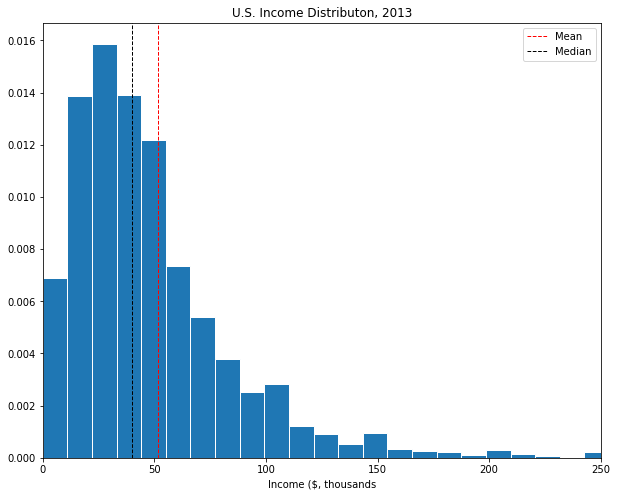
\includegraphics{notebooks/W07. Distributions and Basic Statistics_files/figure-pdf/cell-24-output-2.png}

}

\end{figure}

\bookmarksetup{startatroot}

\hypertarget{question}{%
\chapter{Question:}\label{question}}

Why is the mean the same as the mean (and the mode)?

Not all probability distributions follow the same logic, though -
sometimes a sample is possible - even likely - even if it is dozens of
times the mean, which for height would be tens of metres tall. More
generally, we can start to unpick the shape of a probability curve using
\emph{moments}.

\bookmarksetup{startatroot}

\hypertarget{asymmetric-distributions}{%
\chapter{Asymmetric Distributions}\label{asymmetric-distributions}}

We won't talk about how we decide what the best fit for a dataset is -
suffice it to say that a Gaussian doesn't always fit the bill. In those
cases, the general curve we're dealing with will have a more complex
form.

(\emph{Sometimes we can know that from the underlying process generating
the data - other times we don't, and it's analysing the shape of the
data that tells us})

\begin{Shaded}
\begin{Highlighting}[]
\NormalTok{x\_val}\OperatorTok{=}\NormalTok{ numpy.linspace(}\DecValTok{0}\NormalTok{,}\DecValTok{15}\NormalTok{,}\DecValTok{100}\NormalTok{)}
\NormalTok{y\_val }\OperatorTok{=}\NormalTok{ (x\_val}\OperatorTok{**}\DecValTok{3}\NormalTok{)}\OperatorTok{*}\NormalTok{numpy.exp(}\OperatorTok{{-}}\NormalTok{x\_val)}
\NormalTok{plt.plot(x\_val,y\_val)}
\NormalTok{plt.xlabel(}\StringTok{\textquotesingle{}Value\textquotesingle{}}\NormalTok{)}
\NormalTok{plt.ylabel(}\StringTok{\textquotesingle{}Frequency\textquotesingle{}}\NormalTok{)}
\end{Highlighting}
\end{Shaded}

\begin{verbatim}
Text(0, 0.5, 'Frequency')
\end{verbatim}

\begin{figure}[H]

{\centering 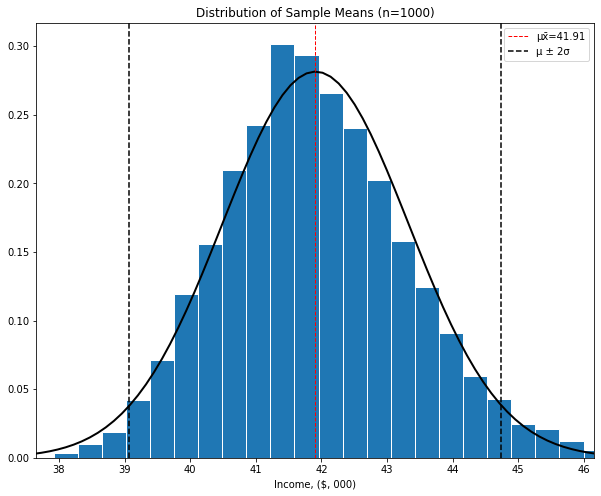
\includegraphics{notebooks/W07. Distributions and Basic Statistics_files/figure-pdf/cell-26-output-2.png}

}

\end{figure}

How do we characterise a dataset which is complex, asymmetric, or we
don't know the underlying form?

\bookmarksetup{startatroot}

\hypertarget{magic-moments}{%
\chapter{Magic Moments}\label{magic-moments}}

Without going into the mathematical detail yet, you can think about
moments as being increasingly nuanced ways of describing distributions.
There are an infinite number of them, but you can understand the first
few inituitively.

\hypertarget{th-moment}{%
\section{0th moment}\label{th-moment}}

0th moment is just area under the curve. In this case it would just be
the number of people sampled. It doesn't tell us much.

\hypertarget{st-moment}{%
\section{1st moment}\label{st-moment}}

1st moment is a central ``tendency'' or average value of the
distribution. In a Gaussian, the mean (average) \(\mu\) is the average
and the centre. But there are other ways of representing this
characteristic, like mode or median, as we will see.

\hypertarget{nd-moment}{%
\section{2nd moment}\label{nd-moment}}

Second moment represents the \emph{width} or \emph{spread} of the curve.
\(\sigma\) is calculated from the second moment, and in a Gaussian
represents the width of the curve. Interquartile range is another way of
doing this, or half-life.

\hypertarget{rd-moment}{%
\section{3rd moment}\label{rd-moment}}

The third moment is related to how \emph{asymmetrical} a curve is, and
the usual way to quantify this is \emph{skewness}. A Gaussian is
symmetric, so its skewness is zero. Actually, all moments apart from 0,
1 and 2 are zero for a Gaussian.

\hypertarget{th-moment-1}{%
\section{4th moment}\label{th-moment-1}}

The standard way to calculate a fourth moment is \emph{Kurtosis}. This
is a measure of how ``peaky'' or ``taily'' a curve is. It's a bit harder
to visualise what we're on about at this point, but it's worth
remembering that a Gaussian has a Kurtosis of 0, so isn't very
``taily''.

\hypertarget{other-moments}{%
\section{Other moments}\label{other-moments}}

It's harder to interpret what they mean, but an arbitrary probability
distribution may need an \emph{infinite} series of moments to be
described correctly. Gaussians are unusual in that they require only two
parameters to describe them; if your data looks Gaussian, that makes
life easier in many ways.

\textbf{Extension}: there are distributions which are simple to write
down that nevertheless are described by an infinite series of moments;
and some, like the Lorentzian, are quite nice functions that have
infinite values for most of their moments.

\hypertarget{recap-the-median}{%
\section{Recap: The Median}\label{recap-the-median}}

The \emph{median} is different from the mean. The median of a data set
is an element that seperates the higher half of the data from the lower
half. For example, the median of \(A = \left \{1,2,3,4,5\right \}\) is
3, and 3 is also the median of \(B = \left \{1,2,3,9,10\right \}\). When
a data set has an even number of members like
\(C = \left \{1,2,3,4\right \}\), the median is defined as the average
of the top lower half and the lower top half, so the median of C is
(2+3)/2=2.5 .

\textbf{Advanced}: How did we define the median from a distribution
(hint: consider area under curve and what it means)? What about
quartiles? What about deciles? What are these quantities?

\hypertarget{exercise-17}{%
\section{Exercise}\label{exercise-17}}

Under which conditions is the median equal to the mean? (hint: look at
the normal distribution - but think more broadly abouting how
``counting'' and ``area under curve'' are related in histograms).

\hypertarget{exercise-18}{%
\section{Exercise}\label{exercise-18}}

Construct a set of 5 numbers such that the median is half the value of
the mean.

\hypertarget{power-laws}{%
\section{Power Laws}\label{power-laws}}

Another type of important distributions are \textbf{power law}
distributions. When the probability of a variable to take the value of
\(x\) is roughly \(\frac{1}{x^k}\) we say that \(x\) has a power law
distribution with exponent \(k\).

For instance let's plot a power law function with exponent 3.

We start off by generating an array of 100 numbers between 1 and 10;
numpy.linspace() lets us do this (here is the documentation if you want
to find out more:
http://docs.scipy.org/doc/numpy/reference/generated/numpy.linspace.html)

\begin{Shaded}
\begin{Highlighting}[]
\NormalTok{x\_val}\OperatorTok{=}\NormalTok{ numpy.linspace(}\DecValTok{1}\NormalTok{,}\DecValTok{10}\NormalTok{,}\DecValTok{100}\NormalTok{)}
\CommentTok{\#** is "to the power of" in Pythonese}
\NormalTok{y\_val }\OperatorTok{=} \DecValTok{1}\OperatorTok{/}\NormalTok{x\_val}\OperatorTok{**}\DecValTok{3}
\NormalTok{plt.plot(x\_val,y\_val)}
\NormalTok{plt.xlabel(}\StringTok{\textquotesingle{}Value\textquotesingle{}}\NormalTok{)}
\NormalTok{plt.ylabel(}\StringTok{\textquotesingle{}Frequency\textquotesingle{}}\NormalTok{)}
\NormalTok{plt.xlim(}\DecValTok{1}\NormalTok{,}\DecValTok{5}\NormalTok{)}
\end{Highlighting}
\end{Shaded}

\begin{verbatim}
(1.0, 5.0)
\end{verbatim}

\begin{figure}[H]

{\centering \includegraphics{notebooks/W07. Distributions and Basic Statistics_files/figure-pdf/cell-29-output-2.png}

}

\end{figure}

An important class of power law distributions are called \textbf{Pareto}
type distributions. Consider for instance, the distribution of income in
a city. We will find that about 20\% of the population has 80\% of the
wealth, this is also known as a 80:20 law.

\begin{Shaded}
\begin{Highlighting}[]
\NormalTok{sample }\OperatorTok{=} \DecValTok{10000}
\NormalTok{exponent }\OperatorTok{=} \DecValTok{3}

\NormalTok{bins }\OperatorTok{=} \DecValTok{1000}


\NormalTok{y }\OperatorTok{=} \DecValTok{1} \OperatorTok{+}\NormalTok{ numpy.random.pareto(exponent, sample)}

\NormalTok{plt.hist(y, bins, histtype}\OperatorTok{=}\StringTok{\textquotesingle{}step\textquotesingle{}}\NormalTok{)}
\NormalTok{plt.xlim((}\DecValTok{1}\NormalTok{, }\DecValTok{5}\NormalTok{))}
\NormalTok{plt.xlabel(}\StringTok{\textquotesingle{}Value\textquotesingle{}}\NormalTok{)}
\NormalTok{plt.ylabel(}\StringTok{\textquotesingle{}Frequency\textquotesingle{}}\NormalTok{)}
\end{Highlighting}
\end{Shaded}

\begin{verbatim}
Text(0, 0.5, 'Frequency')
\end{verbatim}

\begin{figure}[H]

{\centering \includegraphics{notebooks/W07. Distributions and Basic Statistics_files/figure-pdf/cell-30-output-2.png}

}

\end{figure}

\hypertarget{exercise-19}{%
\section{Exercise:}\label{exercise-19}}

Add lines showing the mean, mode and median to the above graph, and
comment on this with a box of markdown.

\hypertarget{comments}{%
\section{Comments:}\label{comments}}

We plotted the mean, mode and median of the distribution\ldots{}

\hypertarget{extension-quantifying-datasets-which-cover-a-wide-range-of-values.}{%
\section{Extension: Quantifying Datasets Which Cover a Wide Range of
Values.}\label{extension-quantifying-datasets-which-cover-a-wide-range-of-values.}}

Objects like the mean present a problem for power laws - in some cases,
they diverge. So, for the mathematicians, if the exponent is 1, we can
approximate the mean by

\(\mu = \int_0^{\infty}dx \frac{1}{x}*x = \int_0^{\infty}dx = \infty\)!

which gives a nonsensical value. Larger exponents (larger than 2) ensure
this doesn't occur - but what sense does the mean make when there are
people earning 10, 100 or 1000 times that mean value?

When datasets cover many orders of magnitude (here from 33 to 2090), we
may need to think about \emph{geometrical} methods for understanding its
properties. For the mean, we might consider the \emph{geometrical mean},
achieved by mutiplying the 100 values together and taking the 100th
root. To understand the width, we might use a half-life type measure.
Half-life is the ``time'' it takes for a radioactive source to reach
half its current level of radioactivity; but we can think about applying
this to other situations, where ``time'' is replaced by ``percentile''
and ``radioactivity'' is replaced by ``income'', for example.

\hypertarget{extension-bimodal-distributions}{%
\section{Extension: Bimodal
Distributions}\label{extension-bimodal-distributions}}

Sometimes distributions are \emph{Bimodal} or multimodal. What this
literally means is that they have multiple ``modes'' - most popular
values - i.e.~peaks. In these cases, mean may not be the best measure
and we may need to think about these two (or larger number of) peaks
relates to different segments of our sample or population.

\begin{Shaded}
\begin{Highlighting}[]
\NormalTok{sample }\OperatorTok{=} \DecValTok{100000}
\NormalTok{a }\OperatorTok{=} \DecValTok{25} \OperatorTok{*}\NormalTok{ numpy.random.randn(sample) }\OperatorTok{+} \DecValTok{20}
\ControlFlowTok{for}\NormalTok{ i }\KeywordTok{in} \BuiltInTok{range}\NormalTok{(}\BuiltInTok{int}\NormalTok{(sample}\OperatorTok{/}\DecValTok{2}\NormalTok{)):}
\NormalTok{    a[i] }\OperatorTok{=}\NormalTok{ a[i]}\OperatorTok{*}\FloatTok{1.3}\OperatorTok{+}\DecValTok{100}
\NormalTok{plt.hist(a, }\DecValTok{250}\NormalTok{, histtype}\OperatorTok{=}\StringTok{\textquotesingle{}step\textquotesingle{}}\NormalTok{)}\OperatorTok{;}
\NormalTok{plt.xlabel(}\StringTok{\textquotesingle{}Value\textquotesingle{}}\NormalTok{)}
\NormalTok{plt.ylabel(}\StringTok{\textquotesingle{}Frequency\textquotesingle{}}\NormalTok{)}
\end{Highlighting}
\end{Shaded}

\begin{verbatim}
Text(0, 0.5, 'Frequency')
\end{verbatim}

\begin{figure}[H]

{\centering \includegraphics{notebooks/W07. Distributions and Basic Statistics_files/figure-pdf/cell-33-output-2.png}

}

\end{figure}

\hypertarget{exercise-20}{%
\section{Exercise:}\label{exercise-20}}

Plot the mean and median for the above graph. What might be better
statistics? How might you find them?

\bookmarksetup{startatroot}

\hypertarget{regression}{%
\chapter{Regression}\label{regression}}

\bookmarksetup{startatroot}

\hypertarget{machine-learning}{%
\chapter{Machine Learning}\label{machine-learning}}

\hypertarget{workshop-9-open-in-colab}{%
\section[\emph{Workshop 9} ]{\texorpdfstring{\emph{Workshop 9}
\href{https://colab.research.google.com/github/oballinger/QM2/blob/main/notebooks/W09.\%20Machine\%20Learning.ipynb}{\protect
\includegraphics{notebooks/../colab-badge.png}}}{Workshop 9 Open In Colab}}\label{workshop-9-open-in-colab}}

This short introduction uses
\href{https://www.tensorflow.org/guide/keras/overview}{Keras} to:

\begin{enumerate}
\def\labelenumi{\arabic{enumi}.}
\tightlist
\item
  Load a prebuilt dataset.
\item
  Build a neural network machine learning model that classifies images.
\item
  Train this neural network.
\item
  Evaluate the accuracy of the model.
\end{enumerate}

\hypertarget{set-up-tensorflow}{%
\section{Set up TensorFlow}\label{set-up-tensorflow}}

Import TensorFlow into your program to get started:

\begin{Shaded}
\begin{Highlighting}[]
\ImportTok{import}\NormalTok{ numpy }\ImportTok{as}\NormalTok{ np}
\ImportTok{import}\NormalTok{ tensorflow }\ImportTok{as}\NormalTok{ tf}
\ImportTok{import}\NormalTok{ matplotlib.pyplot }\ImportTok{as}\NormalTok{ plt}

\BuiltInTok{print}\NormalTok{(}\StringTok{"TensorFlow version:"}\NormalTok{, tf.\_\_version\_\_)}
\end{Highlighting}
\end{Shaded}

\begin{verbatim}
TypeError: Descriptors cannot not be created directly.
If this call came from a _pb2.py file, your generated code is out of date and must be regenerated with protoc >= 3.19.0.
If you cannot immediately regenerate your protos, some other possible workarounds are:
 1. Downgrade the protobuf package to 3.20.x or lower.
 2. Set PROTOCOL_BUFFERS_PYTHON_IMPLEMENTATION=python (but this will use pure-Python parsing and will be much slower).

More information: https://developers.google.com/protocol-buffers/docs/news/2022-05-06#python-updates
\end{verbatim}

If you are following along in your own development environment, rather
than
\href{https://colab.research.google.com/github/tensorflow/docs/blob/master/site/en/tutorials/quickstart/beginner.ipynb}{Colab},
see the \href{https://www.tensorflow.org/install}{install guide} for
setting up TensorFlow for development.

Note: Make sure you have upgraded to the latest \texttt{pip} to install
the TensorFlow 2 package if you are using your own development
environment. See the \href{https://www.tensorflow.org/install}{install
guide} for details.

\hypertarget{load-a-dataset}{%
\section{Load a dataset}\label{load-a-dataset}}

Load and prepare the \href{http://yann.lecun.com/exdb/mnist/}{MNIST
dataset}. Convert the sample data from integers to floating-point
numbers:

\begin{Shaded}
\begin{Highlighting}[]
\NormalTok{mnist }\OperatorTok{=}\NormalTok{ tf.keras.datasets.mnist}

\NormalTok{(x\_train, y\_train), (x\_test, y\_test) }\OperatorTok{=}\NormalTok{ mnist.load\_data()}
\NormalTok{x\_train, x\_test }\OperatorTok{=}\NormalTok{ x\_train }\OperatorTok{/} \FloatTok{255.0}\NormalTok{, x\_test }\OperatorTok{/} \FloatTok{255.0}
\end{Highlighting}
\end{Shaded}

\begin{verbatim}
Downloading data from https://storage.googleapis.com/tensorflow/tf-keras-datasets/mnist.npz
11493376/11490434 [==============================] - 0s 0us/step
11501568/11490434 [==============================] - 0s 0us/step
\end{verbatim}

\begin{Shaded}
\begin{Highlighting}[]

\KeywordTok{def}\NormalTok{ plot\_num(number):}

\NormalTok{  item\_index }\OperatorTok{=}\NormalTok{ np.where(y\_train[:}\DecValTok{1000}\NormalTok{]}\OperatorTok{==}\NormalTok{number)}
\NormalTok{  subset}\OperatorTok{=}\NormalTok{x\_train[item\_index]}
  
\NormalTok{  egs}\OperatorTok{=}\DecValTok{5}
\NormalTok{  fig, axs }\OperatorTok{=}\NormalTok{ plt.subplots(}\DecValTok{1}\NormalTok{,egs, figsize}\OperatorTok{=}\NormalTok{(}\DecValTok{20}\NormalTok{,}\DecValTok{10}\NormalTok{))}

  \ControlFlowTok{for}\NormalTok{ i }\KeywordTok{in} \BuiltInTok{range}\NormalTok{(}\DecValTok{0}\NormalTok{,egs):}
\NormalTok{    axs[i].imshow(subset[i])}


\ControlFlowTok{for}\NormalTok{ x }\KeywordTok{in} \BuiltInTok{range}\NormalTok{(}\DecValTok{0}\NormalTok{,}\DecValTok{10}\NormalTok{):}
\NormalTok{  plot\_num(x)}
\end{Highlighting}
\end{Shaded}

\begin{figure}[H]

{\centering \includegraphics{notebooks/W09. Machine Learning_files/figure-pdf/cell-4-output-1.png}

}

\end{figure}

\begin{figure}[H]

{\centering 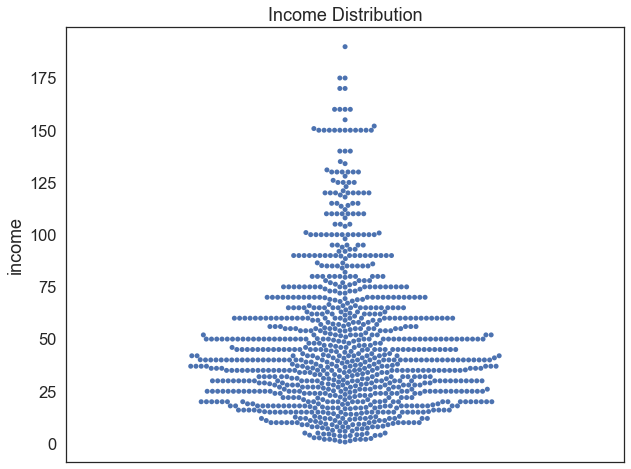
\includegraphics{notebooks/W09. Machine Learning_files/figure-pdf/cell-4-output-2.png}

}

\end{figure}

\begin{figure}[H]

{\centering \includegraphics{notebooks/W09. Machine Learning_files/figure-pdf/cell-4-output-3.png}

}

\end{figure}

\begin{figure}[H]

{\centering \includegraphics{notebooks/W09. Machine Learning_files/figure-pdf/cell-4-output-4.png}

}

\end{figure}

\begin{figure}[H]

{\centering \includegraphics{notebooks/W09. Machine Learning_files/figure-pdf/cell-4-output-5.png}

}

\end{figure}

\begin{figure}[H]

{\centering \includegraphics{notebooks/W09. Machine Learning_files/figure-pdf/cell-4-output-6.png}

}

\end{figure}

\begin{figure}[H]

{\centering \includegraphics{notebooks/W09. Machine Learning_files/figure-pdf/cell-4-output-7.png}

}

\end{figure}

\begin{figure}[H]

{\centering \includegraphics{notebooks/W09. Machine Learning_files/figure-pdf/cell-4-output-8.png}

}

\end{figure}

\begin{figure}[H]

{\centering \includegraphics{notebooks/W09. Machine Learning_files/figure-pdf/cell-4-output-9.png}

}

\end{figure}

\begin{figure}[H]

{\centering \includegraphics{notebooks/W09. Machine Learning_files/figure-pdf/cell-4-output-10.png}

}

\end{figure}

\hypertarget{build-a-machine-learning-model}{%
\section{Build a machine learning
model}\label{build-a-machine-learning-model}}

Build a \texttt{tf.keras.Sequential} model by stacking layers.

\begin{Shaded}
\begin{Highlighting}[]
\NormalTok{model }\OperatorTok{=}\NormalTok{ tf.keras.models.Sequential([}
\NormalTok{  tf.keras.layers.Flatten(input\_shape}\OperatorTok{=}\NormalTok{(}\DecValTok{28}\NormalTok{, }\DecValTok{28}\NormalTok{)),}
\NormalTok{  tf.keras.layers.Dense(}\DecValTok{128}\NormalTok{, activation}\OperatorTok{=}\StringTok{\textquotesingle{}relu\textquotesingle{}}\NormalTok{),}
\NormalTok{  tf.keras.layers.Dropout(}\FloatTok{0.2}\NormalTok{),}
\NormalTok{  tf.keras.layers.Dense(}\DecValTok{10}\NormalTok{)}
\NormalTok{])}
\end{Highlighting}
\end{Shaded}

For each example, the model returns a vector of
\href{https://developers.google.com/machine-learning/glossary\#logits}{logits}
or
\href{https://developers.google.com/machine-learning/glossary\#log-odds}{log-odds}
scores, one for each class.

\begin{Shaded}
\begin{Highlighting}[]
\NormalTok{predictions }\OperatorTok{=}\NormalTok{ model(x\_train[:}\DecValTok{1}\NormalTok{]).numpy()}
\NormalTok{predictions}
\end{Highlighting}
\end{Shaded}

\begin{verbatim}
array([[ 0.33447966,  0.35151538, -0.35632688, -0.2735348 ,  0.8568236 ,
        -0.8503612 , -0.34408805, -0.40424255,  0.4791569 , -0.00873779]],
      dtype=float32)
\end{verbatim}

The \texttt{tf.nn.softmax} function converts these logits to
\emph{probabilities} for each class:

\begin{Shaded}
\begin{Highlighting}[]
\NormalTok{tf.nn.softmax(predictions).numpy()}
\end{Highlighting}
\end{Shaded}

\begin{verbatim}
array([[0.12650587, 0.12867945, 0.06340117, 0.0688737 , 0.21328573,
        0.03868484, 0.06418189, 0.06043489, 0.1461986 , 0.08975388]],
      dtype=float32)
\end{verbatim}

Note: It is possible to bake the \texttt{tf.nn.softmax} function into
the activation function for the last layer of the network. While this
can make the model output more directly interpretable, this approach is
discouraged as it's impossible to provide an exact and numerically
stable loss calculation for all models when using a softmax output.

Define a loss function for training using
\texttt{losses.SparseCategoricalCrossentropy}, which takes a vector of
logits and a \texttt{True} index and returns a scalar loss for each
example.

\begin{Shaded}
\begin{Highlighting}[]
\NormalTok{loss\_fn }\OperatorTok{=}\NormalTok{ tf.keras.losses.SparseCategoricalCrossentropy(from\_logits}\OperatorTok{=}\VariableTok{True}\NormalTok{)}
\end{Highlighting}
\end{Shaded}

This loss is equal to the negative log probability of the true class:
The loss is zero if the model is sure of the correct class.

This untrained model gives probabilities close to random (1/10 for each
class), so the initial loss should be close to
\texttt{-tf.math.log(1/10)\ \textasciitilde{}=\ 2.3}.

\begin{Shaded}
\begin{Highlighting}[]
\NormalTok{loss\_fn(y\_train[:}\DecValTok{1}\NormalTok{], predictions).numpy()}
\end{Highlighting}
\end{Shaded}

\begin{verbatim}
3.2523074
\end{verbatim}

Before you start training, configure and compile the model using Keras
\texttt{Model.compile}. Set the
\href{https://www.tensorflow.org/api_docs/python/tf/keras/optimizers}{\texttt{optimizer}}
class to \texttt{adam}, set the \texttt{loss} to the \texttt{loss\_fn}
function you defined earlier, and specify a metric to be evaluated for
the model by setting the \texttt{metrics} parameter to
\texttt{accuracy}.

\begin{Shaded}
\begin{Highlighting}[]
\NormalTok{model.}\BuiltInTok{compile}\NormalTok{(optimizer}\OperatorTok{=}\StringTok{\textquotesingle{}adam\textquotesingle{}}\NormalTok{,}
\NormalTok{              loss}\OperatorTok{=}\NormalTok{loss\_fn,}
\NormalTok{              metrics}\OperatorTok{=}\NormalTok{[}\StringTok{\textquotesingle{}accuracy\textquotesingle{}}\NormalTok{])}
\end{Highlighting}
\end{Shaded}

\hypertarget{train-and-evaluate-your-model}{%
\section{Train and evaluate your
model}\label{train-and-evaluate-your-model}}

Use the \texttt{Model.fit} method to adjust your model parameters and
minimize the loss:

\begin{Shaded}
\begin{Highlighting}[]
\NormalTok{model.fit(x\_train, y\_train, epochs}\OperatorTok{=}\DecValTok{10}\NormalTok{)}
\end{Highlighting}
\end{Shaded}

\begin{verbatim}
Epoch 1/10
1875/1875 [==============================] - 6s 3ms/step - loss: 0.2955 - accuracy: 0.9139
Epoch 2/10
1875/1875 [==============================] - 5s 3ms/step - loss: 0.1416 - accuracy: 0.9578
Epoch 3/10
1875/1875 [==============================] - 5s 3ms/step - loss: 0.1072 - accuracy: 0.9676
Epoch 4/10
1875/1875 [==============================] - 5s 3ms/step - loss: 0.0874 - accuracy: 0.9727
Epoch 5/10
1875/1875 [==============================] - 5s 3ms/step - loss: 0.0734 - accuracy: 0.9772
Epoch 6/10
1875/1875 [==============================] - 5s 3ms/step - loss: 0.0632 - accuracy: 0.9792
Epoch 7/10
1875/1875 [==============================] - 5s 3ms/step - loss: 0.0575 - accuracy: 0.9808
Epoch 8/10
1875/1875 [==============================] - 5s 3ms/step - loss: 0.0526 - accuracy: 0.9825
Epoch 9/10
1875/1875 [==============================] - 5s 3ms/step - loss: 0.0460 - accuracy: 0.9853
Epoch 10/10
1875/1875 [==============================] - 5s 3ms/step - loss: 0.0437 - accuracy: 0.9858
\end{verbatim}

\begin{verbatim}
<keras.callbacks.History at 0x7fe943384b10>
\end{verbatim}

The \texttt{Model.evaluate} method checks the models performance,
usually on a
``\href{https://developers.google.com/machine-learning/glossary\#validation-set}{Validation-set}''
or
``\href{https://developers.google.com/machine-learning/glossary\#test-set}{Test-set}''.

\begin{Shaded}
\begin{Highlighting}[]
\NormalTok{model.evaluate(x\_test,  y\_test, verbose}\OperatorTok{=}\DecValTok{2}\NormalTok{)}
\end{Highlighting}
\end{Shaded}

\begin{verbatim}
313/313 - 1s - loss: 0.0715 - accuracy: 0.9785 - 529ms/epoch - 2ms/step
\end{verbatim}

\begin{verbatim}
[0.07152838259935379, 0.9785000085830688]
\end{verbatim}

The image classifier is now trained to \textasciitilde98\% accuracy on
this dataset. To learn more, read the
\href{https://www.tensorflow.org/tutorials/}{TensorFlow tutorials}.

If you want your model to return a probability, you can wrap the trained
model, and attach the softmax to it:

\begin{Shaded}
\begin{Highlighting}[]
\NormalTok{probability\_model }\OperatorTok{=}\NormalTok{ tf.keras.Sequential([}
\NormalTok{  model,}
\NormalTok{  tf.keras.layers.Softmax()}
\NormalTok{])}
\end{Highlighting}
\end{Shaded}

\begin{Shaded}
\begin{Highlighting}[]
\CommentTok{\#probability\_model(x\_test[:1])}
\NormalTok{predictions}\OperatorTok{=}\NormalTok{probability\_model.predict(x\_test)}

\NormalTok{index}\OperatorTok{=}\DecValTok{20}

\BuiltInTok{print}\NormalTok{(np.argmax(predictions[index]))}
\NormalTok{plt.imshow(x\_test[index])}
\end{Highlighting}
\end{Shaded}

\begin{verbatim}
9
\end{verbatim}

\begin{verbatim}
<matplotlib.image.AxesImage at 0x7fe9409c1ad0>
\end{verbatim}

\begin{figure}[H]

{\centering \includegraphics{notebooks/W09. Machine Learning_files/figure-pdf/cell-14-output-3.png}

}

\end{figure}

\hypertarget{conclusion}{%
\section{Conclusion}\label{conclusion}}

Congratulations! You have trained a machine learning model using a
prebuilt dataset using the
\href{https://www.tensorflow.org/guide/keras/overview}{Keras} API.

For more examples of using Keras, check out the
\href{https://www.tensorflow.org/tutorials/keras/}{tutorials}. To learn
more about building models with Keras, read the
\href{https://www.tensorflow.org/guide/keras}{guides}. If you want learn
more about loading and preparing data, see the tutorials on
\href{https://www.tensorflow.org/tutorials/load_data/images}{image data
loading} or
\href{https://www.tensorflow.org/tutorials/load_data/csv}{CSV data
loading}.

\bookmarksetup{startatroot}

\hypertarget{advanced-visualization}{%
\chapter{Advanced Visualization}\label{advanced-visualization}}

\hypertarget{workshop-10-open-in-colab}{%
\section[\emph{Workshop 10} ]{\texorpdfstring{\emph{Workshop 10}
\href{https://colab.research.google.com/github/oballinger/QM2/blob/main/notebooks/W10.\%20Advanced\%20Visualization.ipynb}{\protect
\includegraphics{notebooks/../colab-badge.png}}}{Workshop 10 Open In Colab}}\label{workshop-10-open-in-colab}}

We've successfully plotted spatial data using the core pandas and
matplotlib libraries. In this session, we will use \emph{geopandas} - a
library which is designed explicitly to work with apatial data; it does
projection and allows us to plot geometries and create \emph{choropleth}
maps.

\hypertarget{aims-4}{%
\subsection{Aims}\label{aims-4}}

\begin{itemize}
\tightlist
\item
  Create and view a geopandas dataframe
\item
  Understand the significance of the \emph{geometry} column
\item
  The basics of projection
\item
  Create a choropleth map, based on data
\item
  Join dataframes to match data to geographies
\item
  Plot point data (extension)
\item
  Plot point data with a basemap (extension)
\end{itemize}

\hypertarget{install-packages}{%
\section{Install packages}\label{install-packages}}

Firstly, we will need to install Geopandas and pysal so that we can use
it within this workshop. This will generate alot of text and might take
a minute to complete. This is how we install packages within Azure
Notebooks.

\begin{Shaded}
\begin{Highlighting}[]
\CommentTok{\#Install newest branch}
\OperatorTok{!}\NormalTok{pip install pysal}

\CommentTok{\#Install the geopandas module}
\OperatorTok{!}\NormalTok{pip install geopandas}
\end{Highlighting}
\end{Shaded}

\begin{verbatim}
Requirement already satisfied: pysal in /Users/ollieballinger/.pyenv/versions/3.9.5/lib/python3.9/site-packages (2.7.0)
Requirement already satisfied: access>=1.1.8 in /Users/ollieballinger/.pyenv/versions/3.9.5/lib/python3.9/site-packages (from pysal) (1.1.8)
Requirement already satisfied: spaghetti>=1.6.6 in /Users/ollieballinger/.pyenv/versions/3.9.5/lib/python3.9/site-packages (from pysal) (1.6.6)
Requirement already satisfied: mgwr>=2.1.2 in /Users/ollieballinger/.pyenv/versions/3.9.5/lib/python3.9/site-packages (from pysal) (2.1.2)
Requirement already satisfied: spvcm>=0.3.0 in /Users/ollieballinger/.pyenv/versions/3.9.5/lib/python3.9/site-packages (from pysal) (0.3.0)
Requirement already satisfied: momepy>=0.5.3 in /Users/ollieballinger/.pyenv/versions/3.9.5/lib/python3.9/site-packages (from pysal) (0.5.4)
Requirement already satisfied: pointpats>=2.2.0 in /Users/ollieballinger/.pyenv/versions/3.9.5/lib/python3.9/site-packages (from pysal) (2.2.0)
Requirement already satisfied: spint>=1.0.7 in /Users/ollieballinger/.pyenv/versions/3.9.5/lib/python3.9/site-packages (from pysal) (1.0.7)
Requirement already satisfied: libpysal>=4.6.2 in /Users/ollieballinger/.pyenv/versions/3.9.5/lib/python3.9/site-packages (from pysal) (4.6.2)
Requirement already satisfied: spreg>=1.2.4 in /Users/ollieballinger/.pyenv/versions/3.9.5/lib/python3.9/site-packages (from pysal) (1.2.4)
Requirement already satisfied: tobler>=0.8.2 in /Users/ollieballinger/.pyenv/versions/3.9.5/lib/python3.9/site-packages (from pysal) (0.9.0)
Requirement already satisfied: mapclassify>=2.4.3 in /Users/ollieballinger/.pyenv/versions/3.9.5/lib/python3.9/site-packages (from pysal) (2.4.3)
Requirement already satisfied: splot>=1.1.5.post1 in /Users/ollieballinger/.pyenv/versions/3.9.5/lib/python3.9/site-packages (from pysal) (1.1.5.post1)
Requirement already satisfied: spopt>=0.4.1 in /Users/ollieballinger/.pyenv/versions/3.9.5/lib/python3.9/site-packages (from pysal) (0.4.1)
Requirement already satisfied: giddy>=2.3.3 in /Users/ollieballinger/.pyenv/versions/3.9.5/lib/python3.9/site-packages (from pysal) (2.3.3)
Requirement already satisfied: esda>=2.4.1 in /Users/ollieballinger/.pyenv/versions/3.9.5/lib/python3.9/site-packages (from pysal) (2.4.3)
Requirement already satisfied: spglm>=1.0.8 in /Users/ollieballinger/.pyenv/versions/3.9.5/lib/python3.9/site-packages (from pysal) (1.0.8)
Requirement already satisfied: segregation>=2.3.1 in /Users/ollieballinger/.pyenv/versions/3.9.5/lib/python3.9/site-packages (from pysal) (2.3.1)
Requirement already satisfied: inequality>=1.0.0 in /Users/ollieballinger/.pyenv/versions/3.9.5/lib/python3.9/site-packages (from pysal) (1.0.0)
Requirement already satisfied: pandas>=0.23.4 in /Users/ollieballinger/.pyenv/versions/3.9.5/lib/python3.9/site-packages (from access>=1.1.8->pysal) (1.2.4)
Requirement already satisfied: numpy>=1.3 in /Users/ollieballinger/.pyenv/versions/3.9.5/lib/python3.9/site-packages (from access>=1.1.8->pysal) (1.19.5)
Requirement already satisfied: geopandas in /Users/ollieballinger/.pyenv/versions/3.9.5/lib/python3.9/site-packages (from access>=1.1.8->pysal) (0.11.1)
Requirement already satisfied: requests>=2 in /Users/ollieballinger/.pyenv/versions/3.9.5/lib/python3.9/site-packages (from access>=1.1.8->pysal) (2.25.1)
Requirement already satisfied: scipy>=0.11 in /Users/ollieballinger/.pyenv/versions/3.9.5/lib/python3.9/site-packages (from esda>=2.4.1->pysal) (1.6.3)
Requirement already satisfied: scikit-learn in /Users/ollieballinger/.pyenv/versions/3.9.5/lib/python3.9/site-packages (from esda>=2.4.1->pysal) (0.24.2)
Requirement already satisfied: quantecon>=0.4.7 in /Users/ollieballinger/.pyenv/versions/3.9.5/lib/python3.9/site-packages (from giddy>=2.3.3->pysal) (0.5.3)
Requirement already satisfied: beautifulsoup4 in /Users/ollieballinger/.pyenv/versions/3.9.5/lib/python3.9/site-packages (from libpysal>=4.6.2->pysal) (4.9.3)
Requirement already satisfied: jinja2 in /Users/ollieballinger/.pyenv/versions/3.9.5/lib/python3.9/site-packages (from libpysal>=4.6.2->pysal) (3.1.2)
Requirement already satisfied: appdirs in /Users/ollieballinger/.pyenv/versions/3.9.5/lib/python3.9/site-packages (from libpysal>=4.6.2->pysal) (1.4.4)
Requirement already satisfied: packaging in /Users/ollieballinger/.pyenv/versions/3.9.5/lib/python3.9/site-packages (from libpysal>=4.6.2->pysal) (21.3)
Requirement already satisfied: networkx in /Users/ollieballinger/.pyenv/versions/3.9.5/lib/python3.9/site-packages (from mapclassify>=2.4.3->pysal) (2.5.1)
Requirement already satisfied: pygeos in /Users/ollieballinger/.pyenv/versions/3.9.5/lib/python3.9/site-packages (from momepy>=0.5.3->pysal) (0.13)
Requirement already satisfied: tqdm>=4.27.0 in /Users/ollieballinger/.pyenv/versions/3.9.5/lib/python3.9/site-packages (from momepy>=0.5.3->pysal) (4.61.0)
Requirement already satisfied: shapely<2,>=1.7 in /Users/ollieballinger/.pyenv/versions/3.9.5/lib/python3.9/site-packages (from geopandas->access>=1.1.8->pysal) (1.8.4)
Requirement already satisfied: pyproj>=2.6.1.post1 in /Users/ollieballinger/.pyenv/versions/3.9.5/lib/python3.9/site-packages (from geopandas->access>=1.1.8->pysal) (3.4.0)
Requirement already satisfied: fiona>=1.8 in /Users/ollieballinger/.pyenv/versions/3.9.5/lib/python3.9/site-packages (from geopandas->access>=1.1.8->pysal) (1.8.21)
Requirement already satisfied: certifi in /Users/ollieballinger/.pyenv/versions/3.9.5/lib/python3.9/site-packages (from fiona>=1.8->geopandas->access>=1.1.8->pysal) (2020.12.5)
Requirement already satisfied: munch in /Users/ollieballinger/.pyenv/versions/3.9.5/lib/python3.9/site-packages (from fiona>=1.8->geopandas->access>=1.1.8->pysal) (2.5.0)
Requirement already satisfied: cligj>=0.5 in /Users/ollieballinger/.pyenv/versions/3.9.5/lib/python3.9/site-packages (from fiona>=1.8->geopandas->access>=1.1.8->pysal) (0.7.2)
Requirement already satisfied: click>=4.0 in /Users/ollieballinger/.pyenv/versions/3.9.5/lib/python3.9/site-packages (from fiona>=1.8->geopandas->access>=1.1.8->pysal) (8.0.1)
Requirement already satisfied: click-plugins>=1.0 in /Users/ollieballinger/.pyenv/versions/3.9.5/lib/python3.9/site-packages (from fiona>=1.8->geopandas->access>=1.1.8->pysal) (1.1.1)
Requirement already satisfied: attrs>=17 in /Users/ollieballinger/.pyenv/versions/3.9.5/lib/python3.9/site-packages (from fiona>=1.8->geopandas->access>=1.1.8->pysal) (22.1.0)
Requirement already satisfied: six>=1.7 in /Users/ollieballinger/.pyenv/versions/3.9.5/lib/python3.9/site-packages (from fiona>=1.8->geopandas->access>=1.1.8->pysal) (1.15.0)
Requirement already satisfied: setuptools in /Users/ollieballinger/.pyenv/versions/3.9.5/lib/python3.9/site-packages (from fiona>=1.8->geopandas->access>=1.1.8->pysal) (56.0.0)
Requirement already satisfied: decorator<5,>=4.3 in /Users/ollieballinger/.pyenv/versions/3.9.5/lib/python3.9/site-packages (from networkx->mapclassify>=2.4.3->pysal) (4.4.2)
Requirement already satisfied: python-dateutil>=2.7.3 in /Users/ollieballinger/.pyenv/versions/3.9.5/lib/python3.9/site-packages (from pandas>=0.23.4->access>=1.1.8->pysal) (2.8.2)
Requirement already satisfied: pytz>=2017.3 in /Users/ollieballinger/.pyenv/versions/3.9.5/lib/python3.9/site-packages (from pandas>=0.23.4->access>=1.1.8->pysal) (2021.1)
Requirement already satisfied: matplotlib in /Users/ollieballinger/.pyenv/versions/3.9.5/lib/python3.9/site-packages (from pointpats>=2.2.0->pysal) (3.4.2)
Requirement already satisfied: opencv-contrib-python>=4.2.0 in /Users/ollieballinger/.pyenv/versions/3.9.5/lib/python3.9/site-packages (from pointpats>=2.2.0->pysal) (4.6.0.66)
Requirement already satisfied: numba in /Users/ollieballinger/.pyenv/versions/3.9.5/lib/python3.9/site-packages (from quantecon>=0.4.7->giddy>=2.3.3->pysal) (0.56.2)
Requirement already satisfied: sympy in /Users/ollieballinger/.pyenv/versions/3.9.5/lib/python3.9/site-packages (from quantecon>=0.4.7->giddy>=2.3.3->pysal) (1.11.1)
Requirement already satisfied: urllib3<1.27,>=1.21.1 in /Users/ollieballinger/.pyenv/versions/3.9.5/lib/python3.9/site-packages (from requests>=2->access>=1.1.8->pysal) (1.26.5)
Requirement already satisfied: idna<3,>=2.5 in /Users/ollieballinger/.pyenv/versions/3.9.5/lib/python3.9/site-packages (from requests>=2->access>=1.1.8->pysal) (2.10)
Requirement already satisfied: chardet<5,>=3.0.2 in /Users/ollieballinger/.pyenv/versions/3.9.5/lib/python3.9/site-packages (from requests>=2->access>=1.1.8->pysal) (4.0.0)
Requirement already satisfied: rvlib>=0.0.5 in /Users/ollieballinger/.pyenv/versions/3.9.5/lib/python3.9/site-packages (from segregation>=2.3.1->pysal) (0.0.6)
Requirement already satisfied: quilt3 in /Users/ollieballinger/.pyenv/versions/3.9.5/lib/python3.9/site-packages (from segregation>=2.3.1->pysal) (5.0.0)
Requirement already satisfied: joblib in /Users/ollieballinger/.pyenv/versions/3.9.5/lib/python3.9/site-packages (from segregation>=2.3.1->pysal) (1.0.1)
Requirement already satisfied: seaborn in /Users/ollieballinger/.pyenv/versions/3.9.5/lib/python3.9/site-packages (from segregation>=2.3.1->pysal) (0.12.0)
Requirement already satisfied: deprecation in /Users/ollieballinger/.pyenv/versions/3.9.5/lib/python3.9/site-packages (from segregation>=2.3.1->pysal) (2.1.0)
Requirement already satisfied: pip in /Users/ollieballinger/.pyenv/versions/3.9.5/lib/python3.9/site-packages (from segregation>=2.3.1->pysal) (21.1.2)
Requirement already satisfied: cffi>=1.0.0 in /Users/ollieballinger/.pyenv/versions/3.9.5/lib/python3.9/site-packages (from rvlib>=0.0.5->segregation>=2.3.1->pysal) (1.15.1)
Requirement already satisfied: PyYAML in /Users/ollieballinger/.pyenv/versions/3.9.5/lib/python3.9/site-packages (from rvlib>=0.0.5->segregation>=2.3.1->pysal) (5.4.1)
Requirement already satisfied: pycparser in /Users/ollieballinger/.pyenv/versions/3.9.5/lib/python3.9/site-packages (from cffi>=1.0.0->rvlib>=0.0.5->segregation>=2.3.1->pysal) (2.21)
Requirement already satisfied: llvmlite<0.40,>=0.39.0dev0 in /Users/ollieballinger/.pyenv/versions/3.9.5/lib/python3.9/site-packages (from numba->quantecon>=0.4.7->giddy>=2.3.3->pysal) (0.39.1)
Requirement already satisfied: threadpoolctl>=2.0.0 in /Users/ollieballinger/.pyenv/versions/3.9.5/lib/python3.9/site-packages (from scikit-learn->esda>=2.4.1->pysal) (2.1.0)
Requirement already satisfied: rtree in /Users/ollieballinger/.pyenv/versions/3.9.5/lib/python3.9/site-packages (from spaghetti>=1.6.6->pysal) (1.0.0)
Requirement already satisfied: pulp in /Users/ollieballinger/.pyenv/versions/3.9.5/lib/python3.9/site-packages (from spopt>=0.4.1->pysal) (2.6.0)
Requirement already satisfied: statsmodels in /Users/ollieballinger/.pyenv/versions/3.9.5/lib/python3.9/site-packages (from tobler>=0.8.2->pysal) (0.13.2)
Requirement already satisfied: rasterio in /Users/ollieballinger/.pyenv/versions/3.9.5/lib/python3.9/site-packages (from tobler>=0.8.2->pysal) (1.3.2)
Requirement already satisfied: rasterstats in /Users/ollieballinger/.pyenv/versions/3.9.5/lib/python3.9/site-packages (from tobler>=0.8.2->pysal) (0.17.0)
Requirement already satisfied: soupsieve>1.2 in /Users/ollieballinger/.pyenv/versions/3.9.5/lib/python3.9/site-packages (from beautifulsoup4->libpysal>=4.6.2->pysal) (2.2.1)
Requirement already satisfied: MarkupSafe>=2.0 in /Users/ollieballinger/.pyenv/versions/3.9.5/lib/python3.9/site-packages (from jinja2->libpysal>=4.6.2->pysal) (2.0.1)
Requirement already satisfied: pillow>=6.2.0 in /Users/ollieballinger/.pyenv/versions/3.9.5/lib/python3.9/site-packages (from matplotlib->pointpats>=2.2.0->pysal) (8.2.0)
Requirement already satisfied: kiwisolver>=1.0.1 in /Users/ollieballinger/.pyenv/versions/3.9.5/lib/python3.9/site-packages (from matplotlib->pointpats>=2.2.0->pysal) (1.3.1)
Requirement already satisfied: cycler>=0.10 in /Users/ollieballinger/.pyenv/versions/3.9.5/lib/python3.9/site-packages (from matplotlib->pointpats>=2.2.0->pysal) (0.10.0)
Requirement already satisfied: pyparsing>=2.2.1 in /Users/ollieballinger/.pyenv/versions/3.9.5/lib/python3.9/site-packages (from matplotlib->pointpats>=2.2.0->pysal) (2.4.7)
Requirement already satisfied: jsonschema<5,>=3 in /Users/ollieballinger/.pyenv/versions/3.9.5/lib/python3.9/site-packages (from quilt3->segregation>=2.3.1->pysal) (4.16.0)
Requirement already satisfied: boto3>=1.10.0 in /Users/ollieballinger/.pyenv/versions/3.9.5/lib/python3.9/site-packages (from quilt3->segregation>=2.3.1->pysal) (1.24.89)
Requirement already satisfied: tenacity>=5.1.1 in /Users/ollieballinger/.pyenv/versions/3.9.5/lib/python3.9/site-packages (from quilt3->segregation>=2.3.1->pysal) (8.1.0)
Requirement already satisfied: jsonlines==1.2.0 in /Users/ollieballinger/.pyenv/versions/3.9.5/lib/python3.9/site-packages (from quilt3->segregation>=2.3.1->pysal) (1.2.0)
Requirement already satisfied: requests-futures==1.0.0 in /Users/ollieballinger/.pyenv/versions/3.9.5/lib/python3.9/site-packages (from quilt3->segregation>=2.3.1->pysal) (1.0.0)
Requirement already satisfied: aws-requests-auth>=0.4.2 in /Users/ollieballinger/.pyenv/versions/3.9.5/lib/python3.9/site-packages (from quilt3->segregation>=2.3.1->pysal) (0.4.3)
Requirement already satisfied: jmespath<2.0.0,>=0.7.1 in /Users/ollieballinger/.pyenv/versions/3.9.5/lib/python3.9/site-packages (from boto3>=1.10.0->quilt3->segregation>=2.3.1->pysal) (1.0.1)
Requirement already satisfied: botocore<1.28.0,>=1.27.89 in /Users/ollieballinger/.pyenv/versions/3.9.5/lib/python3.9/site-packages (from boto3>=1.10.0->quilt3->segregation>=2.3.1->pysal) (1.27.89)
Requirement already satisfied: s3transfer<0.7.0,>=0.6.0 in /Users/ollieballinger/.pyenv/versions/3.9.5/lib/python3.9/site-packages (from boto3>=1.10.0->quilt3->segregation>=2.3.1->pysal) (0.6.0)
Requirement already satisfied: pyrsistent!=0.17.0,!=0.17.1,!=0.17.2,>=0.14.0 in /Users/ollieballinger/.pyenv/versions/3.9.5/lib/python3.9/site-packages (from jsonschema<5,>=3->quilt3->segregation>=2.3.1->pysal) (0.18.1)
Requirement already satisfied: affine in /Users/ollieballinger/.pyenv/versions/3.9.5/lib/python3.9/site-packages (from rasterio->tobler>=0.8.2->pysal) (2.3.1)
Requirement already satisfied: snuggs>=1.4.1 in /Users/ollieballinger/.pyenv/versions/3.9.5/lib/python3.9/site-packages (from rasterio->tobler>=0.8.2->pysal) (1.4.7)
Requirement already satisfied: simplejson in /Users/ollieballinger/.pyenv/versions/3.9.5/lib/python3.9/site-packages (from rasterstats->tobler>=0.8.2->pysal) (3.17.6)
Requirement already satisfied: patsy>=0.5.2 in /Users/ollieballinger/.pyenv/versions/3.9.5/lib/python3.9/site-packages (from statsmodels->tobler>=0.8.2->pysal) (0.5.3)
Requirement already satisfied: mpmath>=0.19 in /Users/ollieballinger/.pyenv/versions/3.9.5/lib/python3.9/site-packages (from sympy->quantecon>=0.4.7->giddy>=2.3.3->pysal) (1.2.1)
WARNING: You are using pip version 21.1.2; however, version 22.2.2 is available.
You should consider upgrading via the '/Users/ollieballinger/.pyenv/versions/3.9.5/bin/python3.9 -m pip install --upgrade pip' command.
Requirement already satisfied: geopandas in /Users/ollieballinger/.pyenv/versions/3.9.5/lib/python3.9/site-packages (0.11.1)
Requirement already satisfied: pyproj>=2.6.1.post1 in /Users/ollieballinger/.pyenv/versions/3.9.5/lib/python3.9/site-packages (from geopandas) (3.4.0)
Requirement already satisfied: shapely<2,>=1.7 in /Users/ollieballinger/.pyenv/versions/3.9.5/lib/python3.9/site-packages (from geopandas) (1.8.4)
Requirement already satisfied: fiona>=1.8 in /Users/ollieballinger/.pyenv/versions/3.9.5/lib/python3.9/site-packages (from geopandas) (1.8.21)
Requirement already satisfied: pandas>=1.0.0 in /Users/ollieballinger/.pyenv/versions/3.9.5/lib/python3.9/site-packages (from geopandas) (1.2.4)
Requirement already satisfied: packaging in /Users/ollieballinger/.pyenv/versions/3.9.5/lib/python3.9/site-packages (from geopandas) (21.3)
Requirement already satisfied: six>=1.7 in /Users/ollieballinger/.pyenv/versions/3.9.5/lib/python3.9/site-packages (from fiona>=1.8->geopandas) (1.15.0)
Requirement already satisfied: click>=4.0 in /Users/ollieballinger/.pyenv/versions/3.9.5/lib/python3.9/site-packages (from fiona>=1.8->geopandas) (8.0.1)
Requirement already satisfied: certifi in /Users/ollieballinger/.pyenv/versions/3.9.5/lib/python3.9/site-packages (from fiona>=1.8->geopandas) (2020.12.5)
Requirement already satisfied: munch in /Users/ollieballinger/.pyenv/versions/3.9.5/lib/python3.9/site-packages (from fiona>=1.8->geopandas) (2.5.0)
Requirement already satisfied: cligj>=0.5 in /Users/ollieballinger/.pyenv/versions/3.9.5/lib/python3.9/site-packages (from fiona>=1.8->geopandas) (0.7.2)
Requirement already satisfied: click-plugins>=1.0 in /Users/ollieballinger/.pyenv/versions/3.9.5/lib/python3.9/site-packages (from fiona>=1.8->geopandas) (1.1.1)
Requirement already satisfied: setuptools in /Users/ollieballinger/.pyenv/versions/3.9.5/lib/python3.9/site-packages (from fiona>=1.8->geopandas) (56.0.0)
Requirement already satisfied: attrs>=17 in /Users/ollieballinger/.pyenv/versions/3.9.5/lib/python3.9/site-packages (from fiona>=1.8->geopandas) (22.1.0)
Requirement already satisfied: numpy>=1.16.5 in /Users/ollieballinger/.pyenv/versions/3.9.5/lib/python3.9/site-packages (from pandas>=1.0.0->geopandas) (1.19.5)
Requirement already satisfied: pytz>=2017.3 in /Users/ollieballinger/.pyenv/versions/3.9.5/lib/python3.9/site-packages (from pandas>=1.0.0->geopandas) (2021.1)
Requirement already satisfied: python-dateutil>=2.7.3 in /Users/ollieballinger/.pyenv/versions/3.9.5/lib/python3.9/site-packages (from pandas>=1.0.0->geopandas) (2.8.2)
Requirement already satisfied: pyparsing!=3.0.5,>=2.0.2 in /Users/ollieballinger/.pyenv/versions/3.9.5/lib/python3.9/site-packages (from packaging->geopandas) (2.4.7)
WARNING: You are using pip version 21.1.2; however, version 22.2.2 is available.
You should consider upgrading via the '/Users/ollieballinger/.pyenv/versions/3.9.5/bin/python3.9 -m pip install --upgrade pip' command.
\end{verbatim}

\hypertarget{downloading-the-data-3}{%
\section{Downloading the Data}\label{downloading-the-data-3}}

Let's grab the data we will need this week from our course website and
save it into our data folder. If you've not already created a data
folder then do so using the following command.

Don't worry if it generates an error, that means you've already got a
data folder.

\begin{Shaded}
\begin{Highlighting}[]
\OperatorTok{!}\NormalTok{mkdir data}
\end{Highlighting}
\end{Shaded}

\begin{verbatim}
mkdir: data: File exists
\end{verbatim}

\begin{Shaded}
\begin{Highlighting}[]
\OperatorTok{!}\NormalTok{mkdir data}\OperatorTok{/}\NormalTok{wk10}
\OperatorTok{!}\NormalTok{curl https:}\OperatorTok{//}\NormalTok{s3.eu}\OperatorTok{{-}}\NormalTok{west}\OperatorTok{{-}}\FloatTok{2.}\ErrorTok{amazonaws}\NormalTok{.com}\OperatorTok{/}\NormalTok{qm2}\OperatorTok{/}\NormalTok{wk9}\OperatorTok{/}\NormalTok{london\_wards.shp }\OperatorTok{{-}}\NormalTok{o .}\OperatorTok{/}\NormalTok{data}\OperatorTok{/}\NormalTok{wk10}\OperatorTok{/}\NormalTok{london\_wards.shp}
\OperatorTok{!}\NormalTok{curl https:}\OperatorTok{//}\NormalTok{s3.eu}\OperatorTok{{-}}\NormalTok{west}\OperatorTok{{-}}\FloatTok{2.}\ErrorTok{amazonaws}\NormalTok{.com}\OperatorTok{/}\NormalTok{qm2}\OperatorTok{/}\NormalTok{wk9}\OperatorTok{/}\NormalTok{london\_wards.cpg }\OperatorTok{{-}}\NormalTok{o .}\OperatorTok{/}\NormalTok{data}\OperatorTok{/}\NormalTok{wk10}\OperatorTok{/}\NormalTok{london\_wards.cpg}
\OperatorTok{!}\NormalTok{curl https:}\OperatorTok{//}\NormalTok{s3.eu}\OperatorTok{{-}}\NormalTok{west}\OperatorTok{{-}}\FloatTok{2.}\ErrorTok{amazonaws}\NormalTok{.com}\OperatorTok{/}\NormalTok{qm2}\OperatorTok{/}\NormalTok{wk9}\OperatorTok{/}\NormalTok{london\_wards.dbf }\OperatorTok{{-}}\NormalTok{o .}\OperatorTok{/}\NormalTok{data}\OperatorTok{/}\NormalTok{wk10}\OperatorTok{/}\NormalTok{london\_wards.dbf}
\OperatorTok{!}\NormalTok{curl https:}\OperatorTok{//}\NormalTok{s3.eu}\OperatorTok{{-}}\NormalTok{west}\OperatorTok{{-}}\FloatTok{2.}\ErrorTok{amazonaws}\NormalTok{.com}\OperatorTok{/}\NormalTok{qm2}\OperatorTok{/}\NormalTok{wk9}\OperatorTok{/}\NormalTok{london\_wards.prj }\OperatorTok{{-}}\NormalTok{o .}\OperatorTok{/}\NormalTok{data}\OperatorTok{/}\NormalTok{wk10}\OperatorTok{/}\NormalTok{london\_wards.prj}
\OperatorTok{!}\NormalTok{curl https:}\OperatorTok{//}\NormalTok{s3.eu}\OperatorTok{{-}}\NormalTok{west}\OperatorTok{{-}}\FloatTok{2.}\ErrorTok{amazonaws}\NormalTok{.com}\OperatorTok{/}\NormalTok{qm2}\OperatorTok{/}\NormalTok{wk9}\OperatorTok{/}\NormalTok{london\_wards.shx }\OperatorTok{{-}}\NormalTok{o .}\OperatorTok{/}\NormalTok{data}\OperatorTok{/}\NormalTok{wk10}\OperatorTok{/}\NormalTok{london\_wards.shx}
\OperatorTok{!}\NormalTok{curl https:}\OperatorTok{//}\NormalTok{s3.eu}\OperatorTok{{-}}\NormalTok{west}\OperatorTok{{-}}\FloatTok{2.}\ErrorTok{amazonaws}\NormalTok{.com}\OperatorTok{/}\NormalTok{qm2}\OperatorTok{/}\NormalTok{wk9}\OperatorTok{/}\DecValTok{2011}\ErrorTok{persons}\NormalTok{.csv }\OperatorTok{{-}}\NormalTok{o .}\OperatorTok{/}\NormalTok{data}\OperatorTok{/}\NormalTok{wk10}\OperatorTok{/}\DecValTok{2011}\ErrorTok{persons}\NormalTok{.csv}
\OperatorTok{!}\NormalTok{curl https:}\OperatorTok{//}\NormalTok{s3.eu}\OperatorTok{{-}}\NormalTok{west}\OperatorTok{{-}}\FloatTok{2.}\ErrorTok{amazonaws}\NormalTok{.com}\OperatorTok{/}\NormalTok{qm2}\OperatorTok{/}\NormalTok{wk9}\OperatorTok{/}\NormalTok{borough\_density.csv }\OperatorTok{{-}}\NormalTok{o .}\OperatorTok{/}\NormalTok{data}\OperatorTok{/}\NormalTok{wk10}\OperatorTok{/}\NormalTok{borough\_density.csv}
\OperatorTok{!}\NormalTok{curl https:}\OperatorTok{//}\NormalTok{s3.eu}\OperatorTok{{-}}\NormalTok{west}\OperatorTok{{-}}\FloatTok{2.}\ErrorTok{amazonaws}\NormalTok{.com}\OperatorTok{/}\NormalTok{qm2}\OperatorTok{/}\NormalTok{wk9}\OperatorTok{/}\NormalTok{tweet\_data.csv }\OperatorTok{{-}}\NormalTok{o .}\OperatorTok{/}\NormalTok{data}\OperatorTok{/}\NormalTok{wk10}\OperatorTok{/}\NormalTok{tweet\_data.csv}
\end{Highlighting}
\end{Shaded}

\begin{verbatim}
mkdir: data/wk10: File exists
  % Total    % Received % Xferd  Average Speed   Time    Time     Time  Current
                                 Dload  Upload   Total   Spent    Left  Speed
100 2532k  100 2532k    0     0  1562k      0  0:00:01  0:00:01 --:--:-- 1568k
  % Total    % Received % Xferd  Average Speed   Time    Time     Time  Current
                                 Dload  Upload   Total   Spent    Left  Speed
100    10  100    10    0     0    127      0 --:--:-- --:--:-- --:--:--   135
  % Total    % Received % Xferd  Average Speed   Time    Time     Time  Current
                                 Dload  Upload   Total   Spent    Left  Speed
100  201k  100  201k    0     0  1151k      0 --:--:-- --:--:-- --:--:-- 1235k
  % Total    % Received % Xferd  Average Speed   Time    Time     Time  Current
                                 Dload  Upload   Total   Spent    Left  Speed
100   143  100   143    0     0    268      0 --:--:-- --:--:-- --:--:--   271
  % Total    % Received % Xferd  Average Speed   Time    Time     Time  Current
                                 Dload  Upload   Total   Spent    Left  Speed
100  5292  100  5292    0     0  11176      0 --:--:-- --:--:-- --:--:-- 11307
  % Total    % Received % Xferd  Average Speed   Time    Time     Time  Current
                                 Dload  Upload   Total   Spent    Left  Speed
100 1004k  100 1004k    0     0  2439k      0 --:--:-- --:--:-- --:--:-- 2492k
  % Total    % Received % Xferd  Average Speed   Time    Time     Time  Current
                                 Dload  Upload   Total   Spent    Left  Speed
100 6157k  100 6157k    0     0  4282k      0  0:00:01  0:00:01 --:--:-- 4299k
  % Total    % Received % Xferd  Average Speed   Time    Time     Time  Current
                                 Dload  Upload   Total   Spent    Left  Speed
100  156k  100  156k    0     0   833k      0 --:--:-- --:--:-- --:--:--  861k
\end{verbatim}

\hypertarget{setup-our-enviroment}{%
\section{Setup our enviroment}\label{setup-our-enviroment}}

\begin{Shaded}
\begin{Highlighting}[]
\OperatorTok{!}\NormalTok{pip install descartes}
\OperatorTok{!}\NormalTok{pip install mapclassify}
\end{Highlighting}
\end{Shaded}

\begin{verbatim}
Requirement already satisfied: descartes in /Users/ollieballinger/.pyenv/versions/3.9.5/lib/python3.9/site-packages (1.1.0)
Requirement already satisfied: matplotlib in /Users/ollieballinger/.pyenv/versions/3.9.5/lib/python3.9/site-packages (from descartes) (3.4.2)
Requirement already satisfied: pillow>=6.2.0 in /Users/ollieballinger/.pyenv/versions/3.9.5/lib/python3.9/site-packages (from matplotlib->descartes) (8.2.0)
Requirement already satisfied: numpy>=1.16 in /Users/ollieballinger/.pyenv/versions/3.9.5/lib/python3.9/site-packages (from matplotlib->descartes) (1.19.5)
Requirement already satisfied: python-dateutil>=2.7 in /Users/ollieballinger/.pyenv/versions/3.9.5/lib/python3.9/site-packages (from matplotlib->descartes) (2.8.2)
Requirement already satisfied: cycler>=0.10 in /Users/ollieballinger/.pyenv/versions/3.9.5/lib/python3.9/site-packages (from matplotlib->descartes) (0.10.0)
Requirement already satisfied: pyparsing>=2.2.1 in /Users/ollieballinger/.pyenv/versions/3.9.5/lib/python3.9/site-packages (from matplotlib->descartes) (2.4.7)
Requirement already satisfied: kiwisolver>=1.0.1 in /Users/ollieballinger/.pyenv/versions/3.9.5/lib/python3.9/site-packages (from matplotlib->descartes) (1.3.1)
Requirement already satisfied: six in /Users/ollieballinger/.pyenv/versions/3.9.5/lib/python3.9/site-packages (from cycler>=0.10->matplotlib->descartes) (1.15.0)
WARNING: You are using pip version 21.1.2; however, version 22.2.2 is available.
You should consider upgrading via the '/Users/ollieballinger/.pyenv/versions/3.9.5/bin/python3.9 -m pip install --upgrade pip' command.
Requirement already satisfied: mapclassify in /Users/ollieballinger/.pyenv/versions/3.9.5/lib/python3.9/site-packages (2.4.3)
Requirement already satisfied: pandas>=1.0 in /Users/ollieballinger/.pyenv/versions/3.9.5/lib/python3.9/site-packages (from mapclassify) (1.2.4)
Requirement already satisfied: numpy>=1.3 in /Users/ollieballinger/.pyenv/versions/3.9.5/lib/python3.9/site-packages (from mapclassify) (1.19.5)
Requirement already satisfied: networkx in /Users/ollieballinger/.pyenv/versions/3.9.5/lib/python3.9/site-packages (from mapclassify) (2.5.1)
Requirement already satisfied: scikit-learn in /Users/ollieballinger/.pyenv/versions/3.9.5/lib/python3.9/site-packages (from mapclassify) (0.24.2)
Requirement already satisfied: scipy>=1.0 in /Users/ollieballinger/.pyenv/versions/3.9.5/lib/python3.9/site-packages (from mapclassify) (1.6.3)
Requirement already satisfied: python-dateutil>=2.7.3 in /Users/ollieballinger/.pyenv/versions/3.9.5/lib/python3.9/site-packages (from pandas>=1.0->mapclassify) (2.8.2)
Requirement already satisfied: pytz>=2017.3 in /Users/ollieballinger/.pyenv/versions/3.9.5/lib/python3.9/site-packages (from pandas>=1.0->mapclassify) (2021.1)
Requirement already satisfied: six>=1.5 in /Users/ollieballinger/.pyenv/versions/3.9.5/lib/python3.9/site-packages (from python-dateutil>=2.7.3->pandas>=1.0->mapclassify) (1.15.0)
Requirement already satisfied: decorator<5,>=4.3 in /Users/ollieballinger/.pyenv/versions/3.9.5/lib/python3.9/site-packages (from networkx->mapclassify) (4.4.2)
Requirement already satisfied: threadpoolctl>=2.0.0 in /Users/ollieballinger/.pyenv/versions/3.9.5/lib/python3.9/site-packages (from scikit-learn->mapclassify) (2.1.0)
Requirement already satisfied: joblib>=0.11 in /Users/ollieballinger/.pyenv/versions/3.9.5/lib/python3.9/site-packages (from scikit-learn->mapclassify) (1.0.1)
WARNING: You are using pip version 21.1.2; however, version 22.2.2 is available.
You should consider upgrading via the '/Users/ollieballinger/.pyenv/versions/3.9.5/bin/python3.9 -m pip install --upgrade pip' command.
\end{verbatim}

\begin{Shaded}
\begin{Highlighting}[]
\ImportTok{from}\NormalTok{ pysal }\ImportTok{import} \OperatorTok{*}
\ImportTok{import}\NormalTok{ geopandas }\ImportTok{as}\NormalTok{ gp}
\ImportTok{import}\NormalTok{ pandas }\ImportTok{as}\NormalTok{ pd}
\ImportTok{import}\NormalTok{ matplotlib.pyplot }\ImportTok{as}\NormalTok{ plt}
\ImportTok{import}\NormalTok{ matplotlib}
\ImportTok{import}\NormalTok{ pylab}
\ImportTok{import}\NormalTok{ descartes}
\ImportTok{import}\NormalTok{ mapclassify}

\OperatorTok{\%}\NormalTok{matplotlib inline}

\NormalTok{plt.style.use(}\StringTok{\textquotesingle{}ggplot\textquotesingle{}}\NormalTok{)}
\NormalTok{pylab.rcParams[}\StringTok{\textquotesingle{}figure.figsize\textquotesingle{}}\NormalTok{] }\OperatorTok{=}\NormalTok{ (}\FloatTok{20.}\NormalTok{, }\FloatTok{16.}\NormalTok{)}
\end{Highlighting}
\end{Shaded}

\hypertarget{the-shape-of-things-to-come}{%
\section{The shape of things to
come}\label{the-shape-of-things-to-come}}

Geopandas works with \emph{shapefiles} - an industry standard in spatial
analysis and GIS created by ESRI, who make a lot of GIS products.
Shapefiles actually involves a number of files (\emph{filename.shp},
\emph{filename.shx}, \emph{filename.dbf}, \emph{filename.proj} and
\emph{filename.cpg}) which encode the polygons, data, projection and
various other useful bits of data. Suffice it to say that we generally
need all of these bits, with the same filename (but different
extension), in the same folder. Generally, if you download shapefiles,
it should have all of the requisite bits.

We'll load them into a \emph{GeoDataFrame} object, which, as we will
see, looks a lot like a pandas dataframe - but has a special column,
\emph{geometry}, which is what is used whenever we invoke the ``plot''
command.

Let's load the data - the geometries of London wards:

\begin{Shaded}
\begin{Highlighting}[]
\NormalTok{data\_path }\OperatorTok{=} \StringTok{"./data/wk9/london\_wards.shp"}

\CommentTok{\# londonWards = gp.GeoDataFrame.from\_file(data\_path)}

\NormalTok{londonWards }\OperatorTok{=}\NormalTok{ gp.read\_file(data\_path)}

\NormalTok{londonWards.head()}
\end{Highlighting}
\end{Shaded}

\begin{longtable}[]{@{}lllllllllllllllll@{}}
\toprule()
& NAME & AREA\_CODE & DESCRIPTIO & FILE\_NAME & NUMBER & NUMBER0 &
POLYGON\_ID & UNIT\_ID & CODE & HECTARES & AREA & TYPE\_CODE & DESCRIPT0
& TYPE\_COD0 & DESCRIPT1 & geometry \\
\midrule()
\endhead
0 & Chessington South Ward & LBW & London Borough Ward &
GREATER\_LONDON\_AUTHORITY & 52 & 733 & 50840 & 10884 & E05000405 &
755.173 & 0.0 & VA & CIVIL VOTING AREA & None & None & POLYGON
((-0.33068 51.32901, -0.33059 51.32909... \\
1 & Tolworth and Hook Rise Ward & LBW & London Borough Ward &
GREATER\_LONDON\_AUTHORITY & 106 & 734 & 117160 & 11407 & E05000414 &
259.464 & 0.0 & VA & CIVIL VOTING AREA & None & None & POLYGON
((-0.30846 51.37586, -0.30834 51.37606... \\
2 & Berrylands Ward & LBW & London Borough Ward &
GREATER\_LONDON\_AUTHORITY & 107 & 735 & 50449 & 11413 & E05000401 &
145.390 & 0.0 & VA & CIVIL VOTING AREA & None & None & POLYGON
((-0.30385 51.39249, -0.30375 51.39252... \\
3 & Alexandra Ward & LBW & London Borough Ward &
GREATER\_LONDON\_AUTHORITY & 108 & 736 & 50456 & 11420 & E05000400 &
268.506 & 0.0 & VA & CIVIL VOTING AREA & None & None & POLYGON
((-0.26990 51.38845, -0.26975 51.38838... \\
4 & Beverley Ward & LBW & London Borough Ward &
GREATER\_LONDON\_AUTHORITY & 109 & 737 & 117161 & 11417 & E05000402 &
187.821 & 0.0 & VA & CIVIL VOTING AREA & None & None & POLYGON
((-0.24662 51.39921, -0.24672 51.39921... \\
\bottomrule()
\end{longtable}

\hypertarget{projection}{%
\section{Projection}\label{projection}}

We could spend a long time working through the merits of different
projection methods; many of these are available in geopandas, through
the PySAL library - more documentation is available there if you want to
work with different projections.

More fundamentally, a \emph{Co-ordinate Reference System} (CRS) refers
to how we identify points on the globe; the world isn't a perfect sphere
so dealing with that is the job of the CRS. The WGS84 datum
(https://en.wikipedia.org/wiki/World\_Geodetic\_System) which is
sometimes called EPSG 4326 (epsg:4326).

We can find out the CRS of the geometry:

\begin{Shaded}
\begin{Highlighting}[]
\NormalTok{londonWards.crs}
\end{Highlighting}
\end{Shaded}

\begin{verbatim}
<Geographic 2D CRS: GEOGCS["WGS 84",DATUM["WGS_1984",SPHEROID["WGS 84" ...>
Name: WGS 84
Axis Info [ellipsoidal]:
- lon[east]: Longitude (Degree)
- lat[north]: Latitude (Degree)
Area of Use:
- undefined
Datum: World Geodetic System 1984
- Ellipsoid: WGS 84
- Prime Meridian: Greenwich
\end{verbatim}

If we look at the geometry column, we see that they are latlon
co-ordinates:

\begin{Shaded}
\begin{Highlighting}[]
\NormalTok{londonWards[}\StringTok{\textquotesingle{}geometry\textquotesingle{}}\NormalTok{].head()}
\end{Highlighting}
\end{Shaded}

\begin{verbatim}
0    POLYGON ((-0.33068 51.32901, -0.33059 51.32909...
1    POLYGON ((-0.30846 51.37586, -0.30834 51.37606...
2    POLYGON ((-0.30385 51.39249, -0.30375 51.39252...
3    POLYGON ((-0.26990 51.38845, -0.26975 51.38838...
4    POLYGON ((-0.24662 51.39921, -0.24672 51.39921...
Name: geometry, dtype: geometry
\end{verbatim}

This is all well and good, but we need to project the latlon data onto a
plane to plot. We'll create objects to keep track of these CRS frames.
\emph{original\_crs} is the latlon co-ordinates; \emph{target\_crs} is a
mercator (`merc') projection; and the third line, \emph{to\_crs}
projects the geometry so we can plot it.

\textbf{Extension}: You can find more detailed documentation about
projection types and parameters at the PROJ.4 site which underpins
pyproj/geopandas, and here:
http://www.remotesensing.org/geotiff/proj\_list/; in this case, it won't
make much difference which projection you use, because of the small
scale.

\begin{Shaded}
\begin{Highlighting}[]
\NormalTok{londonWards.crs }\OperatorTok{=} \StringTok{\textquotesingle{}epsg:4326\textquotesingle{}}
\NormalTok{target\_crs }\OperatorTok{=}\NormalTok{ \{}\StringTok{\textquotesingle{}datum\textquotesingle{}}\NormalTok{:}\StringTok{\textquotesingle{}WGS84\textquotesingle{}}\NormalTok{, }\StringTok{\textquotesingle{}no\_defs\textquotesingle{}}\NormalTok{:}\VariableTok{True}\NormalTok{, }\StringTok{\textquotesingle{}proj\textquotesingle{}}\NormalTok{:}\StringTok{\textquotesingle{}merc\textquotesingle{}}\NormalTok{\}}
\NormalTok{projected\_londonWards }\OperatorTok{=}\NormalTok{ londonWards.to\_crs(crs}\OperatorTok{=}\NormalTok{target\_crs)}
\end{Highlighting}
\end{Shaded}

The `geometry' column isn't in a lon, lat CRS any longer, but physical
distances from some spatial point:

\begin{Shaded}
\begin{Highlighting}[]
\NormalTok{projected\_londonWards[}\StringTok{\textquotesingle{}geometry\textquotesingle{}}\NormalTok{].head()}
\end{Highlighting}
\end{Shaded}

\begin{verbatim}
0    POLYGON ((-36811.020 6646318.081, -36801.601 6...
1    POLYGON ((-34337.301 6654646.965, -34324.488 6...
2    POLYGON ((-33824.387 6657604.802, -33813.361 6...
3    POLYGON ((-30045.140 6656886.727, -30028.328 6...
4    POLYGON ((-27453.834 6658801.486, -27465.224 6...
Name: geometry, dtype: geometry
\end{verbatim}

Plotting this is now a simple matter:

\begin{Shaded}
\begin{Highlighting}[]
\NormalTok{projected\_londonWards.plot()}
\end{Highlighting}
\end{Shaded}

\begin{verbatim}
<AxesSubplot:>
\end{verbatim}

\begin{figure}[H]

{\centering 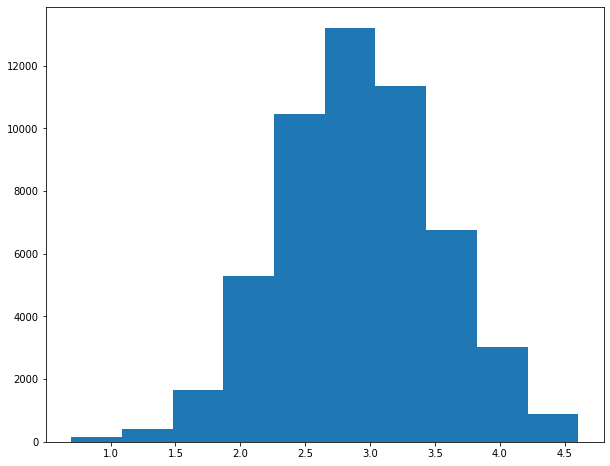
\includegraphics{notebooks/W10. Advanced Visualization_files/figure-pdf/cell-12-output-2.png}

}

\end{figure}

Our colours look a bit plain and boring. Let's upgrade our plot to
something more informative.

\begin{Shaded}
\begin{Highlighting}[]
\NormalTok{projected\_londonWards.plot(column}\OperatorTok{=}\StringTok{\textquotesingle{}UNIT\_ID\textquotesingle{}}\NormalTok{, cmap}\OperatorTok{=}\StringTok{\textquotesingle{}rainbow\textquotesingle{}}\NormalTok{, scheme}\OperatorTok{=}\StringTok{\textquotesingle{}quantiles\textquotesingle{}}\NormalTok{)}
\end{Highlighting}
\end{Shaded}

\begin{verbatim}
<AxesSubplot:>
\end{verbatim}

\begin{figure}[H]

{\centering \includegraphics{notebooks/W10. Advanced Visualization_files/figure-pdf/cell-13-output-2.png}

}

\end{figure}

Have a play around with mapping differnt coloums using different colours
and different colouring schemes

\texttt{Scheme\ must\ be\ in\ the\ set:\ {[}\textquotesingle{}quantiles\textquotesingle{},\ \textquotesingle{}fisher\_jenks\textquotesingle{},\ \textquotesingle{}equal\_interval\textquotesingle{}{]}}

If you want to play with the colour schemes for the map then take a look
here. https://matplotlib.org/examples/color/colormaps\_reference.html

\texttt{Possible\ values\ are:\ Accent,\ Accent\_r,\ Blues,\ Blues\_r,\ BrBG,\ BrBG\_r,\ BuGn,\ BuGn\_r,\ BuPu,\ BuPu\_r,\ CMRmap,\ CMRmap\_r,\ Dark2,\ Dark2\_r,\ GnBu,\ GnBu\_r,\ Greens,\ Greens\_r,\ Greys,\ Greys\_r,\ OrRd,\ OrRd\_r,\ Oranges,\ Oranges\_r,\ PRGn,\ PRGn\_r,\ Paired,\ Paired\_r,\ Pastel1,\ Pastel1\_r,\ Pastel2,\ Pastel2\_r,\ PiYG,\ PiYG\_r,\ PuBu,\ PuBuGn,\ PuBuGn\_r,\ PuBu\_r,\ PuOr,\ PuOr\_r,\ PuRd,\ PuRd\_r,\ Purples,\ Purples\_r,\ RdBu,\ RdBu\_r,\ RdGy,\ RdGy\_r,\ RdPu,\ RdPu\_r,\ RdYlBu,\ RdYlBu\_r,\ RdYlGn,\ RdYlGn\_r,\ Reds,\ Reds\_r,\ Set1,\ Set1\_r,\ Set2,\ Set2\_r,\ Set3,\ Set3\_r,\ Spectral,\ Spectral\_r,\ Wistia,\ Wistia\_r,\ YlGn,\ YlGnBu,\ YlGnBu\_r,\ YlGn\_r,\ YlOrBr,\ YlOrBr\_r,\ YlOrRd,\ YlOrRd\_r,\ afmhot,\ afmhot\_r,\ autumn,\ autumn\_r,\ binary,\ binary\_r,\ bone,\ bone\_r,\ brg,\ brg\_r,\ bwr,\ bwr\_r,\ cool,\ cool\_r,\ coolwarm,\ coolwarm\_r,\ copper,\ copper\_r,\ cubehelix,\ cubehelix\_r,\ flag,\ flag\_r,\ gist\_earth,\ gist\_earth\_r,\ gist\_gray,\ gist\_gray\_r,\ gist\_heat,\ gist\_heat\_r,\ gist\_ncar,\ gist\_ncar\_r,\ gist\_rainbow,\ gist\_rainbow\_r,\ gist\_stern,\ gist\_stern\_r,\ gist\_yarg,\ gist\_yarg\_r,\ gnuplot,\ gnuplot2,\ gnuplot2\_r,\ gnuplot\_r,\ gray,\ gray\_r,\ hot,\ hot\_r,\ hsv,\ hsv\_r,\ inferno,\ inferno\_r,\ jet,\ jet\_r,\ magma,\ magma\_r,\ nipy\_spectral,\ nipy\_spectral\_r,\ ocean,\ ocean\_r,\ pink,\ pink\_r,\ plasma,\ plasma\_r,\ prism,\ prism\_r,\ rainbow,\ rainbow\_r,\ seismic,\ seismic\_r,\ spectral,\ spectral\_r,\ spring,\ spring\_r,\ summer,\ summer\_r,\ terrain,\ terrain\_r,\ viridis,\ viridis\_r,\ winter,\ winter\_r}

We can also control the alpha of the map as well if we want to.

\begin{Shaded}
\begin{Highlighting}[]
\NormalTok{projected\_londonWards.plot(column}\OperatorTok{=}\StringTok{\textquotesingle{}UNIT\_ID\textquotesingle{}}\NormalTok{, cmap}\OperatorTok{=}\StringTok{\textquotesingle{}rainbow\textquotesingle{}}\NormalTok{, scheme}\OperatorTok{=}\StringTok{\textquotesingle{}quantiles\textquotesingle{}}\NormalTok{, alpha }\OperatorTok{=} \FloatTok{0.5}\NormalTok{)}
\end{Highlighting}
\end{Shaded}

\begin{verbatim}
<AxesSubplot:>
\end{verbatim}

\begin{figure}[H]

{\centering 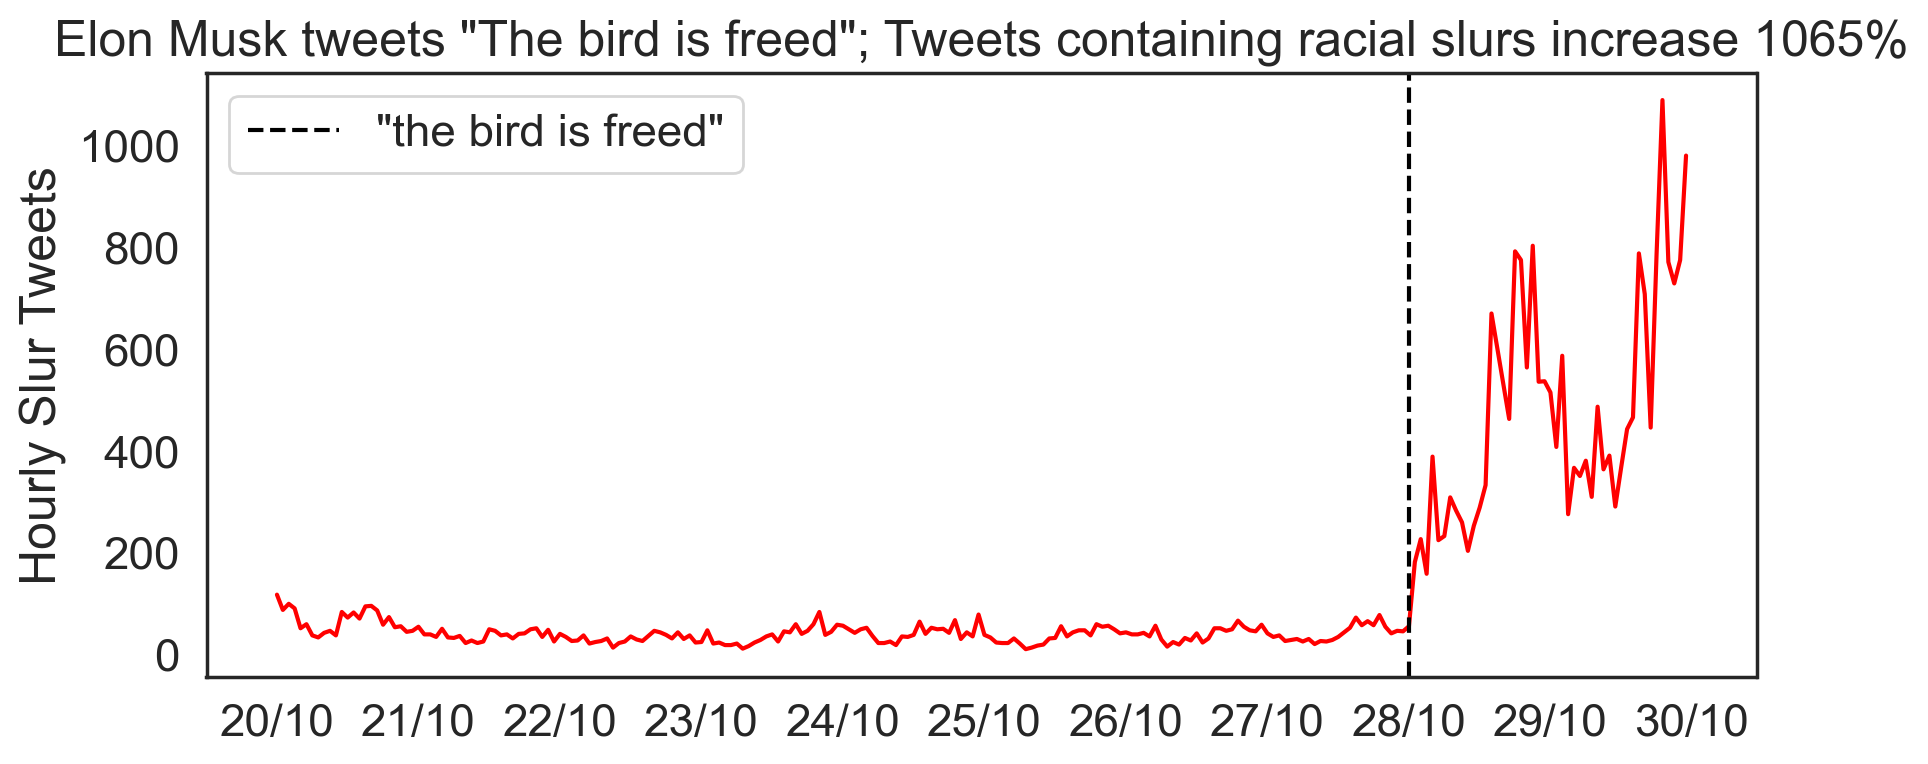
\includegraphics{notebooks/W10. Advanced Visualization_files/figure-pdf/cell-14-output-2.png}

}

\end{figure}

\hypertarget{warding-off-evil}{%
\section{Warding off evil}\label{warding-off-evil}}

The electoral wards of London represent voting areas for local councils;
let's now compare their populations to see where the population
densities are in the city.

Population data is available from the ONS - they link the population of
different ages to a `Ward Code', which is a standard identified of that
ward:
http://www.ons.gov.uk/ons/publications/re-reference-tables.html?edition=tcm\%3A77-301951

Let's read it into a standard Pandas dataframe:

\begin{Shaded}
\begin{Highlighting}[]
\NormalTok{data\_path }\OperatorTok{=} \StringTok{"./data/wk9/2011persons.csv"}

\NormalTok{persons }\OperatorTok{=}\NormalTok{ pd.read\_csv(data\_path, encoding }\OperatorTok{=} \StringTok{\textquotesingle{}latin1\textquotesingle{}}\NormalTok{)}
\NormalTok{persons.head()}
\end{Highlighting}
\end{Shaded}

\begin{longtable}[]{@{}llllllllllllllllllllll@{}}
\toprule()
& Ward Code 1 & Ward Name 1 & Local Authority & All Ages & 0-4 & 5-9 &
10-14 & 15-19 & 20-24 & 25-29 & ... & 45-49 & 50-54 & 55-59 & 60-64 &
65-69 & 70-74 & 75-79 & 80-84 & 85-89 & 90plus \\
\midrule()
\endhead
0 & E05000001 & Aldersgate & City of London & 1,472 & 50 & 36 & 23 & 19
& 66 & 138 & ... & 113 & 109 & 131 & 135 & 73 & 65 & 62 & 48.0 & 19.0 &
8.0 \\
1 & E05000005 & Bishopsgate & City of London & 226 & 2 & 1 & 2 & 6 & 20
& 64 & ... & 13 & 12 & 13 & 8 & 2 & 0 & 0 & 1.0 & 0.0 & 0.0 \\
2 & E05000015 & Cripplegate & City of London & 2,786 & 108 & 66 & 54 &
102 & 117 & 233 & ... & 237 & 212 & 183 & 187 & 163 & 125 & 76 & 93.0 &
43.0 & 31.0 \\
3 & E05000017 & Farringdon Within & City of London & 278 & 8 & 12 & 26 &
9 & 31 & 40 & ... & 17 & 12 & 14 & 13 & 10 & 3 & 1 & 0.0 & 0.0 & 0.0 \\
4 & E05000018 & Farringdon Without & City of London & 1,112 & 17 & 5 & 6
& 6 & 146 & 233 & ... & 106 & 51 & 59 & 67 & 31 & 22 & 11 & 8.0 & 5.0 &
2.0 \\
\bottomrule()
\end{longtable}

We need to make sure the data is in the right format - to remove commas
and dashes, as we have done before. I'm just going to clean up the ``All
Ages'' column for this example, but you could apply this to any (or all)
numerical columns.

\begin{Shaded}
\begin{Highlighting}[]
\NormalTok{persons.replace(}\StringTok{\textquotesingle{},\textquotesingle{}}\NormalTok{, }\StringTok{\textquotesingle{}\textquotesingle{}}\NormalTok{, regex}\OperatorTok{=}\VariableTok{True}\NormalTok{, inplace}\OperatorTok{=}\VariableTok{True}\NormalTok{)}
\NormalTok{persons[}\StringTok{\textquotesingle{}All Ages\textquotesingle{}}\NormalTok{] }\OperatorTok{=}\NormalTok{ persons[}\StringTok{\textquotesingle{}All Ages\textquotesingle{}}\NormalTok{].replace(}\StringTok{\textquotesingle{}{-}\textquotesingle{}}\NormalTok{, }\StringTok{\textquotesingle{}NaN\textquotesingle{}}\NormalTok{, regex}\OperatorTok{=}\VariableTok{True}\NormalTok{).astype(}\StringTok{\textquotesingle{}float\textquotesingle{}}\NormalTok{)}
\NormalTok{persons[}\StringTok{\textquotesingle{}All Ages\textquotesingle{}}\NormalTok{].head()}
\end{Highlighting}
\end{Shaded}

\begin{verbatim}
0    1472.0
1     226.0
2    2786.0
3     278.0
4    1112.0
Name: All Ages, dtype: float64
\end{verbatim}

\hypertarget{exercise-21}{%
\section{Exercise}\label{exercise-21}}

Using the Ward Code, \textbf{merge} the \emph{persons} geodataframe with
the \emph{londonWards} dataframe to create a new geodataframe called
``geopeople''. You can do do this in pretty much exactly the same way
you've done for merging `vanilla' dataframes - refer to the examples
from earlier in the term if your syntax is rusty.

\textbf{One important caveat}: to plot the map, you need to be invoking
\emph{.plot()} on a \textbf{geo}dataframe - so you need to merge
\textbf{on} the geodataframe, with the dataframe as the argument. You
can check this with the \emph{type(geopeople)} command:

\begin{Shaded}
\begin{Highlighting}[]
\BuiltInTok{type}\NormalTok{(geopeople)}
\end{Highlighting}
\end{Shaded}

\begin{verbatim}
NameError: name 'geopeople' is not defined
\end{verbatim}

Compare to merging \textbf{on} persons, which will give you a
``pandas.core.frame.DataFrame'' object - \emph{not} a geodataframe.

Let's now calculate the population \emph{density} using the `HECTARES'
column:

\begin{Shaded}
\begin{Highlighting}[]
\NormalTok{geopeople[}\StringTok{\textquotesingle{}density\textquotesingle{}}\NormalTok{]}\OperatorTok{=}\NormalTok{geopeople[}\StringTok{\textquotesingle{}All Ages\textquotesingle{}}\NormalTok{]}\OperatorTok{/}\NormalTok{geopeople[}\StringTok{\textquotesingle{}HECTARES\textquotesingle{}}\NormalTok{]}
\NormalTok{geopeople.head()}
\end{Highlighting}
\end{Shaded}

\begin{verbatim}
NameError: ignored
\end{verbatim}

\hypertarget{portable-data}{%
\section{Portable data}\label{portable-data}}

At this point, we'll save the data into a .csv so it's easy to use in
other software. This will be useful.

\begin{Shaded}
\begin{Highlighting}[]
\NormalTok{data\_path }\OperatorTok{=} \StringTok{"./data/wk9/borough\_density.csv"}

\NormalTok{geopeople.to\_csv(data\_path)}
\end{Highlighting}
\end{Shaded}

And let's project this into a new geodataframe:

\begin{Shaded}
\begin{Highlighting}[]
\NormalTok{original\_crs }\OperatorTok{=}\NormalTok{ geopeople.crs}
\NormalTok{target\_crs }\OperatorTok{=}\NormalTok{ \{}\StringTok{\textquotesingle{}datum\textquotesingle{}}\NormalTok{:}\StringTok{\textquotesingle{}WGS84\textquotesingle{}}\NormalTok{, }\StringTok{\textquotesingle{}no\_defs\textquotesingle{}}\NormalTok{:}\VariableTok{True}\NormalTok{, }\StringTok{\textquotesingle{}proj\textquotesingle{}}\NormalTok{:}\StringTok{\textquotesingle{}merc\textquotesingle{}}\NormalTok{\}}
\NormalTok{projected\_geopeople }\OperatorTok{=}\NormalTok{ geopeople.to\_crs(crs}\OperatorTok{=}\NormalTok{target\_crs)}
\end{Highlighting}
\end{Shaded}

\begin{Shaded}
\begin{Highlighting}[]
\NormalTok{projected\_geopeople.plot(column}\OperatorTok{=}\StringTok{\textquotesingle{}All Ages\textquotesingle{}}\NormalTok{)}
\NormalTok{plt.title(}\StringTok{\textquotesingle{}2011 population by Ward\textquotesingle{}}\NormalTok{)}
\NormalTok{plt.savefig(}\StringTok{\textquotesingle{}./data/wk9/Wards.png\textquotesingle{}}\NormalTok{)}
\end{Highlighting}
\end{Shaded}

\hypertarget{exercise-22}{%
\section{Exercise}\label{exercise-22}}

Create a choropleth map of the population of each ward using
\emph{projected\_geopeople.plot()} and save it as an image file. Use the
optional arguments:

\begin{enumerate}
\def\labelenumi{\arabic{enumi}.}
\tightlist
\item
  \emph{column}, To specific the `All Ages' column in the dataset to
  colour the map based on population, and
\item
  \emph{colormap}, using the `Blues' colormap to specify a white-blue
  colour range
\end{enumerate}

(It looks as if there aren't population estimates for the smaller City
of London Wards, so we're missing them - if we wanted to show them, we
would need a different dataset)

\hypertarget{between-the-bars}{%
\section{Between the Bars}\label{between-the-bars}}

We have a nice map, but no colour scale to explain what the colours
mean; unfortunately, this is a place where geopandas falls down and we
have to do something intensely complex. The code you'll see below was
created by the inimitable Stephan Hugel to fill in the gaps (more for
the superkeen here:
sensitivecities.com/so-youd-like-to-make-a-map-using-python-EN.html\#.VlSfMcq2-K7)

\begin{Shaded}
\begin{Highlighting}[]
\ImportTok{import}\NormalTok{ numpy }\ImportTok{as}\NormalTok{ np}
\ImportTok{import}\NormalTok{ matplotlib}
\end{Highlighting}
\end{Shaded}

\begin{Shaded}
\begin{Highlighting}[]

\CommentTok{\# Convenience functions for working with colour ramps and bars}
\KeywordTok{def}\NormalTok{ colorbar\_index(ncolors, cmap, labels}\OperatorTok{=}\VariableTok{None}\NormalTok{, }\OperatorTok{**}\NormalTok{kwargs):}
    \CommentTok{"""}
\CommentTok{    This is a convenience function to stop you making off{-}by{-}one errors}
\CommentTok{    Takes a standard colour ramp, and discretizes it,}
\CommentTok{    then draws a colour bar with correctly aligned labels}
\CommentTok{    """}
\NormalTok{    cmap }\OperatorTok{=}\NormalTok{ cmap\_discretize(cmap, ncolors)}
\NormalTok{    mappable }\OperatorTok{=}\NormalTok{ plt.cm.ScalarMappable(cmap}\OperatorTok{=}\NormalTok{cmap)}
\NormalTok{    mappable.set\_array([])}
\NormalTok{    mappable.set\_clim(}\OperatorTok{{-}}\FloatTok{0.5}\NormalTok{, ncolors}\OperatorTok{+}\FloatTok{0.5}\NormalTok{)}
\NormalTok{    colorbar }\OperatorTok{=}\NormalTok{ matplotlib.pyplot.colorbar(mappable, }\OperatorTok{**}\NormalTok{kwargs)}
\NormalTok{    colorbar.set\_ticks(np.linspace(}\DecValTok{0}\NormalTok{, ncolors, ncolors))}
\NormalTok{    colorbar.set\_ticklabels(}\BuiltInTok{range}\NormalTok{(ncolors))}
    \ControlFlowTok{if}\NormalTok{ labels:}
\NormalTok{        colorbar.set\_ticklabels(labels)}
    \ControlFlowTok{return}\NormalTok{ colorbar}

\KeywordTok{def}\NormalTok{ cmap\_discretize(cmap, N):}
    \CommentTok{"""}
\CommentTok{    Return a discrete colormap from the continuous colormap cmap.}

\CommentTok{        cmap: colormap instance, eg. cm.jet. }
\CommentTok{        N: number of colors.}

\CommentTok{    Example}
\CommentTok{        x = resize(arange(100), (5,100))}
\CommentTok{        djet = cmap\_discretize(cm.jet, 5)}
\CommentTok{        imshow(x, cmap=djet)}

\CommentTok{    """}
    \ControlFlowTok{if} \BuiltInTok{type}\NormalTok{(cmap) }\OperatorTok{==} \BuiltInTok{str}\NormalTok{:}
\NormalTok{        cmap }\OperatorTok{=}\NormalTok{ get\_cmap(cmap)}
\NormalTok{    colors\_i }\OperatorTok{=}\NormalTok{ np.concatenate((np.linspace(}\DecValTok{0}\NormalTok{, }\FloatTok{1.}\NormalTok{, N), (}\FloatTok{0.}\NormalTok{, }\FloatTok{0.}\NormalTok{, }\FloatTok{0.}\NormalTok{, }\FloatTok{0.}\NormalTok{)))}
\NormalTok{    colors\_rgba }\OperatorTok{=}\NormalTok{ cmap(colors\_i)}
\NormalTok{    indices }\OperatorTok{=}\NormalTok{ np.linspace(}\DecValTok{0}\NormalTok{, }\FloatTok{1.}\NormalTok{, N }\OperatorTok{+} \DecValTok{1}\NormalTok{)}
\NormalTok{    cdict }\OperatorTok{=}\NormalTok{ \{\}}
    \ControlFlowTok{for}\NormalTok{ ki, key }\KeywordTok{in} \BuiltInTok{enumerate}\NormalTok{((}\StringTok{\textquotesingle{}red\textquotesingle{}}\NormalTok{, }\StringTok{\textquotesingle{}green\textquotesingle{}}\NormalTok{, }\StringTok{\textquotesingle{}blue\textquotesingle{}}\NormalTok{)):}
\NormalTok{        cdict[key] }\OperatorTok{=}\NormalTok{ [(indices[i], colors\_rgba[i }\OperatorTok{{-}} \DecValTok{1}\NormalTok{, ki], colors\_rgba[i, ki]) }\ControlFlowTok{for}\NormalTok{ i }\KeywordTok{in} \BuiltInTok{range}\NormalTok{(N}\OperatorTok{+}\DecValTok{1}\NormalTok{)]}
    \ControlFlowTok{return}\NormalTok{ matplotlib.colors.LinearSegmentedColormap(cmap.name }\OperatorTok{+} \StringTok{"\_}\SpecialCharTok{\%d}\StringTok{"} \OperatorTok{\%}\NormalTok{ N, cdict, }\DecValTok{1024}\NormalTok{)}
\end{Highlighting}
\end{Shaded}

\begin{Shaded}
\begin{Highlighting}[]
\ImportTok{from}\NormalTok{ pysal.viz.mapclassify }\ImportTok{import}\NormalTok{ Quantiles}
\end{Highlighting}
\end{Shaded}

\hypertarget{thems-the-breaks}{%
\section{Them's the breaks}\label{thems-the-breaks}}

There are various ways to split the data, the default of which is
quantiles - to order the data and then split the N data values we have
evenly into q chunks, each of which has N/q data points. Consider the
median - this splits the dataset into two chunks of size N/2; quartiles
split the data into four chunks of size N/4; \emph{quantiles} split the
data into q chunks with N/q points. We will specify 5 chunks using the
k=5 argument.

(The documentation is here, if you're interested in finding out more:
https://github.com/pysal/pysal/blob/master/pysal/contrib/viz/mapping.py)

\begin{Shaded}
\begin{Highlighting}[]
\NormalTok{breaks }\OperatorTok{=}\NormalTok{ Quantiles(geopeople[}\StringTok{\textquotesingle{}density\textquotesingle{}}\NormalTok{].values, k}\OperatorTok{=}\DecValTok{5}\NormalTok{)}
\BuiltInTok{print}\NormalTok{(breaks)}
\end{Highlighting}
\end{Shaded}

\begin{Shaded}
\begin{Highlighting}[]
\BuiltInTok{print}\NormalTok{(breaks.bins)}
\end{Highlighting}
\end{Shaded}

We'll create a set of labels; again, this is a bit beyond what we've
done before so don't worry if it appears a bit mysterious.

\begin{Shaded}
\begin{Highlighting}[]
\NormalTok{bar\_labels }\OperatorTok{=}\NormalTok{ [}\StringTok{\textquotesingle{}\textless{}=}\SpecialCharTok{\%i}\StringTok{\textquotesingle{}}\OperatorTok{\%}\NormalTok{ b }\ControlFlowTok{for}\NormalTok{ b }\KeywordTok{in}\NormalTok{ breaks.bins]}
\BuiltInTok{print}\NormalTok{(bar\_labels)}
\end{Highlighting}
\end{Shaded}

\begin{Shaded}
\begin{Highlighting}[]
\NormalTok{projected\_geopeople.plot(column}\OperatorTok{=}\StringTok{\textquotesingle{}density\textquotesingle{}}\NormalTok{, cmap}\OperatorTok{=}\StringTok{\textquotesingle{}Greens\textquotesingle{}}\NormalTok{, scheme}\OperatorTok{=}\StringTok{\textquotesingle{}quantiles\textquotesingle{}}\NormalTok{, k}\OperatorTok{=}\DecValTok{5}\NormalTok{)}
\NormalTok{plt.title(}\StringTok{\textquotesingle{}2011 population by Ward\textquotesingle{}}\NormalTok{)}

\NormalTok{cmap }\OperatorTok{=}\NormalTok{ plt.get\_cmap(}\StringTok{\textquotesingle{}Greens\textquotesingle{}}\NormalTok{)}
\NormalTok{colorbar\_index(ncolors}\OperatorTok{=}\DecValTok{5}\NormalTok{, cmap}\OperatorTok{=}\NormalTok{cmap, shrink}\OperatorTok{=}\FloatTok{0.5}\NormalTok{, labels}\OperatorTok{=}\NormalTok{bar\_labels)}
\end{Highlighting}
\end{Shaded}

\hypertarget{working-with-point-data-and-choropleths}{%
\section{Working with Point Data and
Choropleths}\label{working-with-point-data-and-choropleths}}

Let's now go back to our twitter data and plot it on the same
axes\ldots{}

\begin{Shaded}
\begin{Highlighting}[]
\NormalTok{data\_path }\OperatorTok{=} \StringTok{"./data/wk9/tweet\_data.csv"}

\NormalTok{tweets }\OperatorTok{=}\NormalTok{ pd.read\_csv(data\_path, parse\_dates }\OperatorTok{=}\NormalTok{ [}\DecValTok{1}\NormalTok{], infer\_datetime\_format }\OperatorTok{=} \VariableTok{True}\NormalTok{, encoding }\OperatorTok{=} \StringTok{\textquotesingle{}latin1\textquotesingle{}}\NormalTok{)}
\NormalTok{tweets.head()}
\end{Highlighting}
\end{Shaded}

We will convert these points to a geometry object - previously, the
geometry column stored data associated with the polygons for the wards -
we'll build geometries representing points and then convert the
dataframe to a geodataframe. Again, the code below is a bit opaque -
it's a recipe for creating these geometries.

\begin{Shaded}
\begin{Highlighting}[]
\ImportTok{from}\NormalTok{ shapely.geometry }\ImportTok{import}\NormalTok{ Point}
\NormalTok{tweets[}\StringTok{\textquotesingle{}geometry\textquotesingle{}}\NormalTok{] }\OperatorTok{=}\NormalTok{ tweets.}\BuiltInTok{apply}\NormalTok{(}\KeywordTok{lambda}\NormalTok{ x: Point(x[}\StringTok{\textquotesingle{}Lon\textquotesingle{}}\NormalTok{], x[}\StringTok{\textquotesingle{}Lat\textquotesingle{}}\NormalTok{]), axis}\OperatorTok{=}\DecValTok{1}\NormalTok{)}
\end{Highlighting}
\end{Shaded}

\hypertarget{project-points-into-the-same-basis}{%
\section{Project points into the same
basis}\label{project-points-into-the-same-basis}}

In the next steps, we will 1) convert the dataframe to a geodataframe.
2) sets the CRS (co-ordinate reference system, remember) to the original
CRS that we got from the wards data, and 3) projects into the same
projection (using mercator, as before)

\begin{Shaded}
\begin{Highlighting}[]
\NormalTok{geotweets }\OperatorTok{=}\NormalTok{ gp.GeoDataFrame(tweets)}
\NormalTok{geotweets.crs }\OperatorTok{=}\NormalTok{ original\_crs}
\NormalTok{geotweets.to\_crs(crs}\OperatorTok{=}\NormalTok{target\_crs, inplace}\OperatorTok{=}\VariableTok{True}\NormalTok{)}
\end{Highlighting}
\end{Shaded}

\begin{Shaded}
\begin{Highlighting}[]
\NormalTok{geotweets.head()}
\end{Highlighting}
\end{Shaded}

\begin{Shaded}
\begin{Highlighting}[]
\NormalTok{geotweets.plot()}
\end{Highlighting}
\end{Shaded}

\begin{Shaded}
\begin{Highlighting}[]
\NormalTok{ax }\OperatorTok{=}\NormalTok{ projected\_geopeople.plot(column}\OperatorTok{=}\StringTok{\textquotesingle{}density\textquotesingle{}}\NormalTok{, cmap}\OperatorTok{=}\StringTok{\textquotesingle{}Greens\textquotesingle{}}\NormalTok{, scheme}\OperatorTok{=}\StringTok{\textquotesingle{}quantiles\textquotesingle{}}\NormalTok{, k}\OperatorTok{=}\DecValTok{5}\NormalTok{)}
\NormalTok{plt.title(}\StringTok{\textquotesingle{}2011 population by Ward\textquotesingle{}}\NormalTok{)}

\NormalTok{cmap }\OperatorTok{=}\NormalTok{ plt.get\_cmap(}\StringTok{\textquotesingle{}Greens\textquotesingle{}}\NormalTok{)}
\NormalTok{colorbar\_index(ncolors}\OperatorTok{=}\DecValTok{5}\NormalTok{, cmap}\OperatorTok{=}\NormalTok{cmap, shrink}\OperatorTok{=}\FloatTok{0.5}\NormalTok{, labels}\OperatorTok{=}\NormalTok{bar\_labels)}

\NormalTok{geotweets.plot(ax}\OperatorTok{=}\NormalTok{ax)}
\end{Highlighting}
\end{Shaded}

\hypertarget{extension-2}{%
\section{Extension:}\label{extension-2}}

We can make these points a bit bigger by using a `buffer' - this creates
a geometry of circles rather than points:

\begin{Shaded}
\begin{Highlighting}[]
\NormalTok{geotweets[}\StringTok{\textquotesingle{}points\textquotesingle{}}\NormalTok{] }\OperatorTok{=}\NormalTok{ geotweets[}\StringTok{\textquotesingle{}geometry\textquotesingle{}}\NormalTok{]}
\NormalTok{geotweets[}\StringTok{\textquotesingle{}geometry\textquotesingle{}}\NormalTok{] }\OperatorTok{=}\NormalTok{ gp.GeoSeries(tweets[}\StringTok{\textquotesingle{}points\textquotesingle{}}\NormalTok{]).}\BuiltInTok{buffer}\NormalTok{(}\DecValTok{200}\NormalTok{)}
\NormalTok{geotweets.head()}
\end{Highlighting}
\end{Shaded}

And we'll add in a dummy variable we can use to make them all the same
colour. Again, a bit clunky but means when we put them on a colormap
(the object which converts a value to a color), it will give the same
colour for each circle.

\begin{Shaded}
\begin{Highlighting}[]
\NormalTok{geotweets[}\StringTok{\textquotesingle{}dummy\textquotesingle{}}\NormalTok{]}\OperatorTok{=}\DecValTok{1}
\end{Highlighting}
\end{Shaded}

Now we can plot this in the same projection, putting geopeople (which
has the borough boundaries) on the same axes as the point twitter data.

\begin{Shaded}
\begin{Highlighting}[]
\NormalTok{ax }\OperatorTok{=}\NormalTok{ projected\_geopeople.plot(column}\OperatorTok{=}\StringTok{\textquotesingle{}density\textquotesingle{}}\NormalTok{, cmap}\OperatorTok{=}\StringTok{\textquotesingle{}Greens\textquotesingle{}}\NormalTok{, scheme}\OperatorTok{=}\StringTok{\textquotesingle{}quantiles\textquotesingle{}}\NormalTok{, k}\OperatorTok{=}\DecValTok{5}\NormalTok{)}
\NormalTok{plt.title(}\StringTok{\textquotesingle{}2011 population by Ward\textquotesingle{}}\NormalTok{)}

\NormalTok{cmap }\OperatorTok{=}\NormalTok{ plt.get\_cmap(}\StringTok{\textquotesingle{}Greens\textquotesingle{}}\NormalTok{)}
\NormalTok{colorbar\_index(ncolors}\OperatorTok{=}\DecValTok{5}\NormalTok{, cmap}\OperatorTok{=}\NormalTok{cmap, shrink}\OperatorTok{=}\FloatTok{0.5}\NormalTok{, labels}\OperatorTok{=}\NormalTok{bar\_labels)}

\NormalTok{geotweets.plot(column}\OperatorTok{=}\StringTok{\textquotesingle{}dummy\textquotesingle{}}\NormalTok{, cmap}\OperatorTok{=}\StringTok{\textquotesingle{}RdBu\textquotesingle{}}\NormalTok{, ax}\OperatorTok{=}\NormalTok{ax)}
\end{Highlighting}
\end{Shaded}

This has been a bit fiddly, but we have a tweet map with a choropleth of
underlying residential population densities. You could look at
evening-time tweets only and then we're starting to get somewhere. But
this is just an example, so you can now use this as a recipe for your
own maps. Or\ldots{}

\hypertarget{alternatives-to-python}{%
\section{Alternatives to Python}\label{alternatives-to-python}}

It's worth experimenting with alternatives if you intend to create more
complex maps. For example, \textbf{Carto} is an option for producing
choropleths. Here is a brief tutorial of how to map population density
based on the csv we created (\emph{borough\_density.csv}) that has the
unprojected borough polygons and their associated population densities.
It's still sensible to do data linking and processing here in python, as
it makes the final stages fairly straightforward - note that Carto works
with latlon (unprojected) data rather than the projected/OSGB data.

\begin{Shaded}
\begin{Highlighting}[]
\ImportTok{from}\NormalTok{ IPython.display }\ImportTok{import}\NormalTok{ YouTubeVideo}
\NormalTok{YouTubeVideo(}\StringTok{"fofRRwZjiyg"}\NormalTok{)}
\end{Highlighting}
\end{Shaded}




\end{document}
